\documentclass[12pt]{report}
\renewcommand{\baselinestretch}{1}
\usepackage{minted}
\usepackage{braket}
\usepackage{wrapfig}
\usepackage{dsfont}
\usepackage[utf8]{inputenc}
\usepackage{amsmath}
\usepackage{graphicx}
\usepackage{subcaption}
\usepackage[left=2.5cm,top=2cm,right=2.5cm,bottom=2.5cm]{geometry}
\usepackage{multicol}
\usepackage{authblk}
\usepackage{subcaption}
\usepackage[backend=bibtex, style=nature]{biblatex}  
\usepackage[toc,page]{appendix}

\usepackage{mwe}
\usepackage{relsize}
\usepackage[font={small,it}]{caption}
\graphicspath{{./img/}}


\usepackage{hyperref}
\hypersetup{
    colorlinks=false, %set true if you want colored links
    linktoc=all,     %set to all if you want both sections and subsections linked
    linkcolor=blue,  %choose some color if you want links to stand out
}


\addbibresource{bibfilename}

%user-defined commands

\newcommand{\qty}[1]
{
	\left({#1}\right)
}

\newcommand{\qtys}[1]
{
	\left[{#1}\right]
}

\newcommand{\qtyc}[1]
{
	\left{{#1}\right}
}

\newcommand{\ssum}
{
	\mathlarger{\sum}
}

\newcommand{\sssum}
{
	\mathlarger{\mathlarger{\sum}}
}
\font\myfont=cmr12 at 16pt


\title{\bf{Nernst-Planck Equation For Electrolytes In The Context Of Copper Electro-refinement.}}

\author{{\myfont Student: Agust\'in Escobar Blanc\\Professor: Enrique Mu\~ noz Tavera}}
\affil{\textit{Departamento de F\'isica, Facultad de F\'isica, Pontificia Universidad Cat\'olica de Chile}}

\begin{document}

\maketitle

\tableofcontents

\newpage
\vspace*{\fill}

\section*{Acknowledgements}

To P. Frez for bearing with me through the harsh moments. To my ever supporting family for the strength. To J. Maze for his guiding advice at the precise moment. To my advisor for his time.

\vspace*{\fill}
\chapter{Diffusion Of Electrolytes In Solution}
\section{Diffusion Processes}


\subsection{Historical Note}

\par Quantitative analysis of transport phenomena was not entirely described up until 1828 with Thomas Graham's experiments on diffusion in gases and liquids \cite{cussler}. Later that century in 1855, Adolf Fick codified the experiments of Graham in what we now know as Fick's Laws. The First Law of Fick's states that the one dimensional flux of a species $i$(that is, the particles per unit time that move through a certain area) is deifined as \cite{cussler}

\begin{align}
\label{eq:fick-fluxes}
	J_i = A j_i = -A\mathcal{D}_i\frac{\partial c_i}{\partial z}.
\end{align}

This is knonw as Fick's fisrt law. Fick was inspired to draw this conclusion from Fourier's work in heat and by the findings of Graham \cite{fick}.


\subsection{Derivation Of Fick's Second Law}

In order to derive Fick's Law for fluxes, we consired diffusion through a thin layer. We want to account for the accumulation of solute within the membrane of Fig. \ref{fig:cussler_thin_layer}. The accumulation should be equal to the rate of diffusion coming into the membrane at $z$ minus the rate at which solute is leaving the membrane at $z+\Delta z$. The sign of the flow is accounted by the fact that particles diffuse from higher concentrations to lower concentrations (from left to right in this case). Therefore,

\begin{align}
	\qty{\textnormal{Solute accumulation in volume }A\Delta z} =& \qty{\textnormal{Rate of diffusion at } z } \nonumber\\
	&- \qty{\textnormal{Rate of diffusion at } z+\Delta z}.\nonumber
\end{align}


Accumulation is by definition the rate of change of the total mass contained in the sample volume $V = A\Delta z$. Therefore

\begin{align}
	\label{eq:derivation-fick-1}
	\frac{\partial \qty{c_1 A\Delta z}}{\partial t} = \qty{J_1 - J_2}.
\end{align}

Where $J_1$ and $J_2$ are the Fick fluxes at $z$ and $z+\Delta z$. Replacing \ref{eq:fick-fluxes} into \ref{eq:derivation-fick-1} and assuming the cross sectional area $A$ is constant

\begin{align}
	\frac{\partial c_1}{\partial t} = \frac{\qty{j_1 - j_2}}{\Delta z},\\
	\frac{\partial c_1}{\partial t} = -\mathcal{D}\frac{\qty{\frac{\Delta c_1}{\Delta z} - \frac{\Delta c_2}{\Delta z}}}{\Delta z}.
\end{align}

As we take $\Delta z \rightarrow 0$ the last equation reduces to

\begin{align}
\label{eq:second-ficks-law}
	\frac{\partial c_1}{\partial t} = \mathcal{D}\frac{\partial^2 c}{\partial z^2}.
\end{align}

\begin{figure}[h!]
\centering
	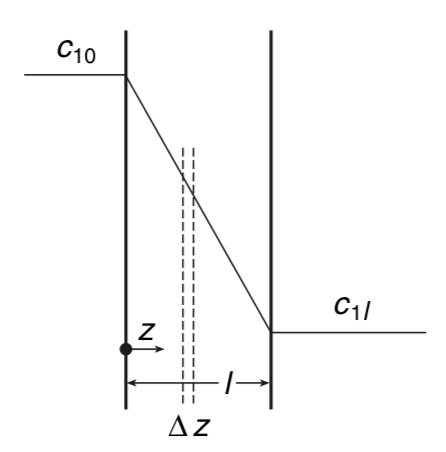
\includegraphics[width=0.5\textwidth]{diffusion_thin_membrane}
	\caption{Diffusion through a thin layer (plot extracted from reference \cite{cussler})}
\label{fig:cussler_thin_layer}
\end{figure}




A particularly interesting solution to equation \ref{eq:second-ficks-law} is that of an initial condition where we have a peak concentration at $x=0$ (such as a drop of substance falling into the underlying fluid at $x=0$). Such inital condition can be stated as

\begin{align}
	c(x,0) = n_0 \delta(x).
\end{align}

The solution to Ficks law is then

\begin{align}
	\label{eq:solution-fick}
	n(x,t) = \frac{2n_0}{\sqrt{\pi}}\int_0^x e^{-\frac{x^2}{4\mathcal{D}t}}.
\end{align}






\subsection{Diffusion Coefficients}

In 1905 Albert Einstein showed that the diffusion of molecules is due to collisions between the suspended particles and the random molecular motion of the medium in which they are suspended \cite{einstein}. 

To understand the physical nature of the diffusion coefficient, one can imagine the setup in which brownian motion was first observed. Let a pollen particle float on water. By close observation with a microscope one finds that the particle starts to move erratically around the center. Nowadays this problem can be studied under the theoretical framework of diffusion of polymers \cite{bird}.

Using arguments from thermodynamics and kinetic theory of gases, Einstein calculated the conditions under which the suspender pollen particle would reach equilibrium states, by minimizing Helmholtz free energy. He found that, if a complementary stochastic force $K$ acts upon a system of $\nu$ particles per unit volume, then at equilibrium

\begin{align}
	-K\nu +\frac{RT}{N}\frac{\partial \nu}{\partial x} = 0.
\end{align} 

Recognizing that osmotic pressure is $p = RT \nu /N$ we get

\begin{align}
\label{eq:einstein-result}
	K\nu - \frac{\partial p}{\partial x},
\end{align}

which shows that equilibrium with force $K$ is bought by osmotic pressure \cite{einstein}. 

With these considerations, we can conclude that the amount of flux produced by the stochastic force $K$ applied to perfectly spherical particles of radius R is

\begin{align}
	j_(x) = -\frac{\nu K}{6\pi u R},
\end{align}

where u is the viscosity of the fluid. From Fick's law the the total flux is given by

\begin{align}
	j(x) = -\mathcal{D}\frac{\partial \nu}{\partial x} = - \frac{\nu K}{6\pi u R},
\end{align}

From Eq. \ref{eq:einstein-result} we get

\begin{align}
\frac{\nu K}{6\pi u R} = \mathcal{D}\frac{N}{RT}\nu K,
\end{align}

Finally, for spherical colloids of radious $R$

\begin{align}
	\mathcal{D} = \frac{RT}{6N\pi u R}.
\end{align}


This is known as the Stokes-Einstein equation and it gives us a physical understanding of how the coefficients fluctuate with temperature and particle size. It is known that this is acurrate to only 20\%, but is still the standard to compute diffusivity coefficients (\cite{cussler}, page 127).









\subsection{Langevin Equation}

Based on Einstien's \cite{einstein} Langevin proposed the motion equations for the polymers in suspention \cite{langevin_translation}. He proposed that, based on the equipartition of kinetic energy among the degrees of freedom of a particular system, the average speed of the particles in the system should be

\begin{align}
	\frac{1}{2}m\bar{v}^2 = \frac{RT}{2N}.
\end{align}

If the particles concidered are big enough (that is, much larger than the average distance between molecules in the fluid) then the particle is subjected to a viscous resistance proportional to the speed of the particle itself

\begin{align}
	\label{eq:friction}
	F_r(x) = -6\pi\mu a \bar{v}.
\end{align}

This however, is an approximation \cite{langevin_original}. Due to impacts of the fluid's constitutive particles the action of the particle oscillates about the value \ref{eq:friction}. Thus, the motion equation of the particle suspended in liquid is

\begin{align}
\label{eq:langevin}
	m\frac{d v}{dt} = -6\pi\mu a v(t) + K(t),
\end{align}

where K is a complementary force induce by the random movement of the particles composing the fluid. This is known as the Langevin equation. 


To gain physical insight of this equation, Langevin \cite{langevin_original} set out to find the variance of the displacement ($\Delta_x^2$) of the particle suspended in liquid. 

The following method is what he used to find $\Delta_x^2$. Multiply by x and write
\begin{align}
	\frac{d}{dt}x^2 = 2x\frac{dx}{dt},\\	
	\frac{d^2}{dt^2}x^2 = 2\qty{x\frac{d^2x}{dt^2}+\qty{\frac{dx},{dt}}^2}
\end{align}


we get the equation

\begin{align}
\label{eq:langevin}
	\frac{m}{2}\qty{\frac{d^2x^2}{dt^2} - 2\qty{\frac{dx}{dt}}^2} = -3\pi\mu a \frac{d x^2}{dt} + K(t)x.
\end{align}

Averaging out the later equation, noticing that $<Kx> = 0$ due to irregularity of the complementary forces $K$ (kicks from the liquid particles come from every direction) and considering the fact that

\begin{align}
	m\qty{\frac{d \bar{x}}{dt}}^2 = \frac{RT}{N}.
\end{align}

Equation \ref{eq:langevin} yields

\begin{align}
	\frac{m}{2}\frac{d^2\bar{x^2}}{dt^2} + 3\pi\mu a \frac{d \bar{x^2}}{dt} = \frac{RT}{N}.
\end{align}

Replacing $z = d\bar{x^2}/dt$ we get

\begin{align}
	\frac{m}{2}\frac{dz}{dt}(z) + 3\pi\mu a z(t) = \frac{RT}{N}.
\end{align}

This equation can be solved for $z$

\begin{align}
	\label{eq:sol-to-langevin}
	z(t) = \frac{RT}{N}\frac{1}{3\pi\mu a} + Ce^{-\frac{6\pi\mu a}{m}t}.
\end{align}

Note from \ref{eq:sol-to-langevin} that the system reaches a steady regime for large $t$. In this regime, we can solve

\begin{align}
	z = \frac{d \bar{x^2}}{dt} =  \frac{RT}{N}\frac{1}{3\pi\mu a},
\end{align}

which gives us

\begin{align}
	\bar{\Delta_x^2} = \bar{x^2} - \bar{x_0^2} =  \frac{RT}{N}\frac{\delta t}{3\pi\mu a},
\end{align}

which is the famous result from Langevin \cite{langevin_original}.











\subsection{Diffusion Of Electrolyte}

In electrolyte diffusion, other forces must be taken into account in order to provide an accurate model. This is because of two main things: One, diffusion of electrolytes is diffusion of at least two types of particles which ionize when disolved in water. Secondly, these charged particles react to possible external electric fields and the electric field produced by the electrolytes themselves.

We know that the flux is given by Fick's law, but this law does not account for the interactions with an electric field. A typical model for the flux of charged particles is

\begin{align}
	j= -\mathcal{D}\qty{\nabla c + \frac{c \mathcal{F}}{RT}\nabla \phi},
\end{align}

which, using Fick's law yield


\begin{align}
\label{eq:nernst-planck}
	\frac{\partial c}{\partial t}= \nabla \cdot D\qty{\nabla c + \frac{c \mathcal{F}}{RT}\nabla \phi},
\end{align}


This is called the Nernst-Planck Equation.

Although Eq. \ref{eq:nernst-planck} accounts for how the diffusion process involves electrical forces in the presence of electrolytes, we haven't accounted as to how the electric field changes due to the presence of electrolytes. 
We start from the Poisson Equation which tells us that

\begin{align}
	\nabla^2 \phi = -\frac{\rho}{\epsilon},
\end{align}

where $\rho$ is the charge distribution. By definition, the charge distribution should be the amount of charge per unit volume, therefore

\begin{align}
	\rho(x,t) = \frac{F}\sum_{s=\pm} z_sc_s,
\end{align}

where $c_s$ is the concentration of each species, $z_s$ is the valence of each species and $\mathcal{F} = N_ae$ is the Faraday constant which is a measure of charge per mol of substance. Therefore, the Poisson equation takes the form

\begin{align}
	\label{eq:poisson-electrolyte}
	\nabla^2 \phi = \frac{F}\sum_{s=\pm} z_sc_s.
\end{align}















\subsection{Copper Electro-refining Process}

Copper ores are highly impure minerals which must be purified in order to meet industry standards of copper production lines in order to maintain desired properties of thermal and electrical conductivity. Electro-refining is the process through which impure copper anodes are dissolved into an electrolyte containing $CuSO_4$ and $H_2SO_4$ to rid the anode from impurities \cite{schlesinger}. Through this process copper anodes can be refined with a purity of $>\%99,997$ $Cu$.


The process of electro-refining can be studied as a redox reaction. The following chemical reactions take place:
\begin{enumerate}
	\item Reduction at the anode: $Cu^{+2}_{(l)} + 2e^- \rightarrow Cu^{0}_{(s)} $  at $V_0 = -0.34V$.
	\item Oxidation at the cathode: $Cu^0_{(s)} \rightarrow Cu^{2+} + 2e^-$at $V_0 = +0.34V$.
\end{enumerate}

To move from anode to cathode, the copper particles migrate by diffusion and convection processes, which have described in previous sections. The net reaction is then

\begin{align}
	Cu_{(impure)} \rightarrow Cu_{(pure)}.
\end{align}

Typical operational concentration of $Cu$ electrolyte are $40-50 g/l = 0.63 M$\cite{schlesinger}. Current per unit area is another parameter of interest. Greater current means faster purification but it could also mean a loss in the purity of the final cathode (due to other metallic impurities in the initial anode such as $Ag$). Nevertheless, operational current of $400 A/m^2$ is routinely achieved in such processes with modern electrolyte flow technology. The operational electrolyte temperature typically ranges from $60 C^0$ to $75 C^0$ celsius.

In electro-refining setups, electrolytes are constantly recirculated at a rate of $\approx 1.2 m^3/h$. Also, other impurities such as $As, Bi, Co, Fe$ among others are present in the purification of copper and do have effects over the speed of the process itself and also the ohmic resistance of the electrolye overall, but these impurities and the recirculation of the electrolyte will be neglected in this work. 


\begin{table}[]
\begin{tabular}{lll}
Parameter & Operational Value & Description                             \\\hline
$C_b$     & $0.63M$           & Concentration of $Cu$                   \\
$i_0$     & $400 A/m^2$       & Current density (current per unit area) \\
$T$       & $70 C^{0}$          & Operational temperature             \\
$V_0$       & $\pm0.3V$          & Operational voltage at anode (-) and cathode(+)             \\\hline   
\end{tabular}
\caption{Table of operational parameters in electro-refining \cite{schlesinger}}
\end{table}
\section{Langmuir Adsorption Model}

Adsorption is a process of adding a particular substance to the surfaces of a solid. This is different than absorption where the substance is actually absorbed into the solid.

Consider the following scenario: we have a substance $B_{(l)}$ in liquid state and $B_{(s)}$ in solid state. The total amount of $B$ substance is

\begin{align}
	VC_B = QC_{(l)} + S C_{(s)}
\end{align}

Since the interaction can only be at the surface, then $V = Q$. Thus,

\begin{align}
	C_{(s)} = \frac{QC_B - QC_{(l)}}{S}
\end{align}

Which yields the amount of substance that is adsorbed to the surface. 

Adsorption depends on the amount of available sites for substance $B$ to attach itself into. The general equation for the reaction is

\begin{align}
	C_{(l)} + \left[\text{Open Sites}\right] \rightleftharpoons C_{(s)}
\end{align} 

Therefore the equilibrium constant for this reaction is

\begin{align}
	K_{eq} = \frac{[C_{(s)}]}{[C_{(l)}][\text{Open Sites}]}
\end{align}

Let $S_T$ be the total number of sites available for this process. The number of total available sites at a given point will be $S_T -C_{(s)}$. Therefore

\begin{align}
	K_{eq} = \frac{[C_{(s)}]}{[C_{(l)}][S_T -C_{(s)}]}
\end{align}

Solving for $C_{(s)}$

\begin{align}
	[C_{(s)}] = \frac{K_{eq}[S_T][C_{(l)}]}{1+K_{eq}[C_{(l)}]}
\end{align} 

To calculate the equilibrium constant of the reaction, we can use the Gibb's free energy, which is

\begin{align}
	\Delta G^0 = -RT \log\qty{K_{eq}}, \\
	\Delta G^0 = -zF V_0,
\end{align}

where $V_0$ is the electrolytic cell's potential and $z$ is the electrolyte's valence. The equilibrium constant can be found to be

\begin{align}
	K_{eq} = \exp\qty{\frac{zF}{RT}V_0}.
\end{align}

Therefore, by knowing the concentration of sites of attachment for $B$ we obtain the adsorption model known as the Langmuir isotherm (it is called an isotherm because the equilibrium constant also depend on temperature) \cite{langmuir}.






\section{Diffusion Of Electrolytes In Electro-refining Context}

We know that electro-refining  apperas to be
\begin{eqnarray}
\frac{\partial C_+}{\partial t}+\nabla\cdot \mathbf{N}_+ = 0, \\
\frac{\partial C_-}{\partial t}+\nabla\cdot \mathbf{N}_- = 0, \\
\nabla^2\phi(x)=-\frac{\rho(x)}{\epsilon}.
\end{eqnarray}
Where $C_s$ is the concentration of each species and $N_s$ is the diffusive flux for each species.
In our model, the flux is defined as

$$\mathbf{N}_+= -D_+\left(\nabla C_+(x) +\frac{z_+ F}{RT}C_+(x)\nabla\phi(x)\right)$$,
$$\mathbf{N}_-= -D_-\left(\nabla C_-(x) +\frac{z_- F}{RT}C_-(x)\nabla\phi(x)\right)$$.

Therefore, the diffusion equation with electric field interaction incorporated is \cite{Dolde2011}

\begin{eqnarray}
\frac{\partial C_+}{\partial t}=\nabla\cdot\left[ \mathcal{D}_+\left(\nabla C_+(x) +\frac{z F}{RT}C_+(x)\nabla\phi(x)\right)\right]= 0, \\
\frac{\partial C_-}{\partial t}=\nabla\cdot\left[ \mathcal{D}_-\left(\nabla C_-(x) -\frac{z F}{RT}C_-(x)\nabla\phi(x)\right)\right] = 0.
\end{eqnarray}

where $z = |z_+|=|z_-|$ is the valence of the electrolyte, $D_{\pm}$ are the diffusion coefficients for each chemical species and $F = 96485.33\,C\,mol^{-1}$ is Faraday's constant.

The reaction we are modeling is the cation reduction. In particular, we are interested in copper reduction at the surface
\begin{equation}
Cu^{+2} + 2 e^{-} \rightarrow Cu^{0}.
\end{equation}

This chemical reaction yields the following border condition for the flux
\begin{eqnarray}
\left.\mathbf{N}_{+}\cdot\hat{n}\right|_{Surface} &=& \frac{I_{0}}{z_{+}FA},\nonumber\\
\left.\mathbf{N}_{-}\cdot\hat{n}\right|_{Surface} &=& 0.
\label{eq_bc1}
\end{eqnarray}

with $A$ being the total area of the surface, $I_{0}$ the total electric current and $\hat{n}$ the unit normal of the surface.
\section{Context Of This Work}
\label{sec:context}
This work is financed by the FONDEF ID $16I10214$ project, which has the main goal of building an electric field sensor to measure quantities related to the electro-refinement of copper. In that context, in this work we will connect the electric field fluctuations to the bulk concentration of copper in the in the electrolytic cell in which this process happens. In order to achieve this goal, an experimental team will use an NV-center based electric field sensor (\cite{Dolde2011}, \cite{NatureMaze}) to measure the noise produced by fluctuation charges ($Cu^{+2}$ and other electrolytes) at the electrode.


\chapter{Review Of Numerical Methods For ODE And PDE Solving}
\section{Runge-Kutta Method}
\label{sec:run_kut}

The Runge-Kutta Method is used to determine the numerical value of a system of differential equations to which we know the boundary conditions. Let 

$$\vec{y}' = \vec{F}(x, \vec{y})$$
$$\vec{y}(x_0) = \vec{y}_0$$

be the system of equations we want to solve with the method. We approximate the derivative by

$$\frac{\vec{y}(x+h)-\vec{y}(x)}{h} = \vec{F}(x + h, \vec{y}+\vec{y}(x+h))$$

We want to approximate the left hand side with a series expansion to arbitrary order in $h$. We obtain thus an expression for $y(x+h)$,

$$\vec{y}(x+h)=\vec{y}(x)+ h\vec{F}(x + h, \vec{y}+\vec{y}(x+h)).$$

In this work we use the Runge-Kutta of fifth order in the integration step $h$. The expression for the increment at this order of precision is

$$\vec{y}_5(x+h) = \vec{y}(x) + \sum_{i=0}^{6} C_{i} K_i,$$

and

$$K_0 = hF(x,y),$$
$$K_i = hF(x+A_ih,y+\sum_{i=0}^{i-1} B_{ij} K_j)$$

where $i = 1,2,3, .. , 6 $.

We also need the fourth order Runge-Kutta method in order to obtain the error in the integration. This is given by

$$\vec{y}_4(x+h) = \vec{y}(x) + \sum_{i=0}^{6} D_{i} K_i,$$

The error is given by 

\begin{eqnarray}
\vec{E}(h) = \vec{y}_5(x+h) - \vec{y}_4(x+h).
\end{eqnarray}

Of this expression, we can take the root mean square of the components of $\vec{E}(h)$,

\begin{equation}
e(h) = \sqrt{\frac{1}{n}\sum_{i=0}^{n-1}E_i^2(h)}
\end{equation}

This way we obtain a scalar measure of the error.

If $h_1$ and $h_2$ are two consecutive steps in the integration of the differential equation, then it can be shown that

\begin{equation}
\frac{e(h_1)}{e(h_2)} \approx \qty{\frac{h_1}{h_2}}^5
\label{eq:error}
\end{equation}

We don't know what the error of the next step will be, but we can define a tolerance $\epsilon>0$ such that the error of the next step is at most $\epsilon$. Thus, the following step can be computed from Eq. \ref{eq:error} by letting $e(h_2) = \epsilon$

\begin{equation}
h_2= h_1\qty{\frac{\epsilon}{e(h_1)}}^{1/5}
\label{eq:error}
\end{equation}

This method is good for our purposes since the curves we are trying to analyze are flat at the begining but have sharp slopes towards the interface (see Fig. \ref{fig:concentration} and \ref{fig:firstorderphi}).

\section{The Shooting Method}

The method described in section \ref{sec:run_kut} can solve the system of equations if the border conditions are all known at a given value of $x = x_0$. Nevertheless, as it can be seen from \ref{eq:border-conditions},
that we have boundary conditions at $x=0$ (the interface) and at $x=\delta$ the bulk solution (see Fig. \ref{fig:geometry}). This is a complication which can be overcome by using the shooting method. The idea is to transform the problem with boundary conditions 

$$C_+(\delta) = C_-(\delta) = C_b$$
$$\phi(\delta) = 0$$
$$\phi(0) = V_0$$

into the problem


$$C_+(\delta) = C_-(\delta) = C_b$$
$$\phi(\delta) = 0$$
$$E(\delta) = u,$$

where $u$ is a constant yet to be determined. To determine $u$, we define a residual function

$$r(u) = \phi(0)-V_0.$$

which is zero when the valueof $\phi(0)$ (given an appropriate u) is the original boundary condition. Therefore, the two-point boundary problem is transformed into a  root finding problem. First, we need to find two values of $u$, $u_1$ and $u_2$ such that $r(u_1) < 0$ and  $r(u_2) > 0$. Once we have that, we can use Ridder's method to find the root.

\section{Ridder's Method}

In this method it is assumed that the root is bracketed within to values.  We define an auxiliary function 
$$G(x) = F(x)e^{(x-x1)Q}$$
where $Q$ is determined by imposing that the points $(x_1, G(x_1))$, $(x_2, G(x_2))$ and $(x_3, G(x_3))$ be in a straight line. That is, if $x_1-x_2 = 2h$ and f $x_1-x_3 = h = x_3-x_2$ we should get

\begin{equation}
G(x_3) = \frac{G(x_1)-G(x_2)}{2}.
\label{eq:line-requirement}
\end{equation}

Using equation \ref{eq:line-requirement}, we obtain that

\begin{eqnarray}
e^{hQ} = \frac{f(x_1)+f(x_2)e^{2hQ}}{2}
\end{eqnarray}

Which is a quadratic equation on $e^{hQ}$. Solving for this quantity we obtain

\begin{equation}
e^{hQ} = \frac{f(x_3)\pm\sqrt{f(x_3)^2-f(x_2)f(x_1)}}{f(x_2)}
\end{equation}

Now that we have determined completely our function $G(x)$, we can do linear interpolation on it to get a better estimation of the root of f(x). Let $x_r$  be it. Then

$$x_r^{\pm} = x_3 \pm (x_3-x_1)\frac{f(x_3)}{\sqrt{f^2(x_3)-f(x_1)f(x_2)}}$$

It can be show that 
\begin{itemize}
\item If $f(x_1)-f(x_2) < 0$, we should pick the $x_r^-$ solution
\item If $f(x_1)-f(x_2) > 0$, we should pick the $x_r^+$ solution
\end{itemize}

When we have our solution, we make $x_3 = x_r^{s}$ ($s+,-$, for every case) and find a new correction to $x_r$. We stop when $x_r^+-x_r^-$ is below the define tolerance.

To test convergence, out method assumes the function we are passing on is of the form

$$f(x) = g(x) -g_0,$$

where we are trying to find $x_0$ such that $g(x_0) = g_0$. This means that when the root is found, we should get 

$$f(x_0) \in [-\epsilon,+\epsilon],$$

where $\epsilon>0$ is a predefined tolerance.


\section{Finite Difference Methods}

\par Finite difference methods are based on the fact that functions can be approximated by polinomials (Taylor theorem) \cite{kiusalaas}. In what is known as the forward difference scheme, a function $f$ can be written as

\begin{align}
	\label{eq:forward-difference}
	f(x_{i+1})=f(x_i) + hf (x_i) + \frac{h^2}{2!} f''(x_i)\mathcal{O}(h^3).
\end{align}

where $h = (x_{max}-x_{min})/M$ and $x_{i+1} = x_i$. Other  schemes are the backward 

\begin{align}
\label{eq:backward-difference}
	f(x_{i-1})=f(x_i) - hf (x_i) + + \frac{h^2}{2!} f''(x_i)\mathcal{O}(h^3),
\end{align}

and the central difference scheme


\begin{align}
\label{eq:central-difference}
	f(x_{i-1}) + f(x_{i+1})= 2f(x_i) + hf''(x_i) + \mathcal{O}(h^4),
\end{align}


There are several ways to define the derivative acording to equations \label{eq:backward-difference}, \label{eq:forward-difference} and \label{eq:central-difference} this but they all follow the same principles: partition the integration interval in $M$ intervals and compute derivatives of functions at each point as the subtraction of the neighboring terms. Thus we can approximate a function's derivative in three different ways

\begin{align}
	f'(x_i) &= \frac{f(x_{i+1})-f(x_{i})}{h} + \mathcal{O}(h^2),\\
	f'(x_i) &= \frac{f(x_{i})-f(x_{i-1})}{h} + \mathcal{O}(h^2),\\
	f'(x_i) &= \frac{f(x_{i+1})-f(x_{i-1})}{2h} + \mathcal{O}(h^2)
\end{align}

which are called the first forward, backward and central difference approximations respectively. 
Second derivatives can be computed in a similar manner

\begin{align}
	f''(x_i) &= \frac{f(x_{i+2})-2f(x_{i+1})+f(x_{i+1})}{h^2} + \mathcal{O}(h^2),\\
	f''(x_i) &= \frac{f(x_{i-2})-2f(x_{i-1})+f(x_i)}{h^2} + \mathcal{O}(h^2),\\
	f''(x_i) &= \frac{f(x_{i+1})-2f(x_i)+f(x_{i-1})}{h^2} + \mathcal{O}(h^2)
\end{align}

Usually, operators $\mathcal{D_+}$, $\mathcal{D_-}$ and $\mathcal{D_0}$ are defined such that

\begin{align}
	\label{eq:differnece-operators}
	D_+f(x_i) &= \frac{f(x_{i+2})-2f(x_{i+1})+f(x_{i+1})}{h^2},\\
	D_-f(x_i) &= \frac{f(x_{i-2})-2f(x_{i-1})+f(x_i)}{h^2},\\
	D_0f(x_i) &= \frac{f(x_{i+1})-2f(x_i)+f(x_{i-1})}{h^2}
\end{align}


\subsection{Error In Finite Difference Methods}


In the above approximated derivatives we have assumed we'll expand up to first order in $h$. For general order $h^p$ error we should expect it to behave as \cite{leveque_ch1}

\begin{align}
	E(h)\approx Ch^p,
\end{align}

or equivalently

\begin{align}
	\log\qty{E(h)}\approx \log\qty{C}+p\log{\qty{h}}.
\end{align}

In figure \ref{fig:leveque_errors_plotting} a plot is given of the error in computing \ref{eq:differnece-operators} in terms of the parameter $h$



\begin{figure}[h!]
\centering
	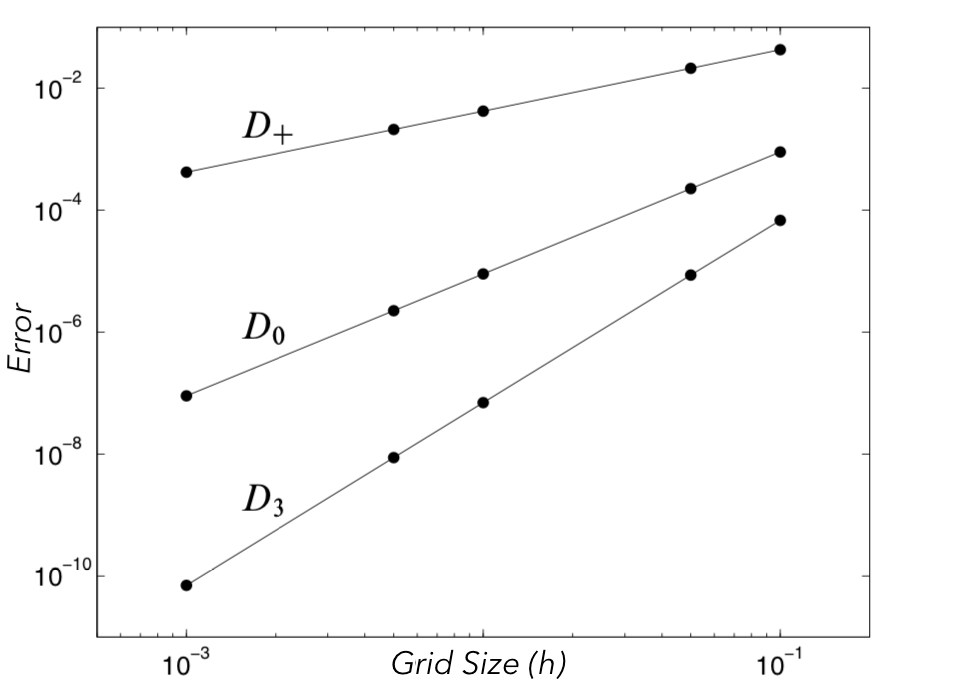
\includegraphics[width=0.5\textwidth]{leveque_errors_plotting}
	\caption{Plotting error for the different numerical differentiation schemes (plot extracted from reference \cite{leveque_ch1})}
\label{fig:leveque_errors_plotting}
\end{figure}


\section{Applying Finite Difference Methods to PDEs}

For one dimensional diffusion-like equations

\begin{align}
\frac{\partial f}{\partial t} &= \frac{\partial^2 f}{\partial x^2} + F(x, f(x), f'(x)).
\label{eq:finite-difference}
\end{align}

We will discretize the derivative as described in \ref{eq:forward-difference} and replacing 

\begin{align}
	f(t_n, x_k) = \rho^{n,k},
\end{align}

which yields the following derivation rules for temporal and spacial derivatives
\begin{align}
\frac{\partial \rho}{\partial \tau}^{n+1, k}= \frac{C^{n+1, k}-\rho^{n, k}}{\Delta t},\\
\frac{\partial^2 \rho}{\partial x^2}^{n+1, k} = \frac{\rho^{n+1, k-1}-2\rho^{n, k}+\rho^{n+1, k+1}}{\Delta \xi^2}.
\end{align}

Replacing these approximations into equation \ref{eq:diffusion} we get

\begin{align}	
\label{eq:linear-eq-numeric}
    -\alpha \rho^{n+1,k-1} + ( 1 + 2\alpha ) \rho^{n+1,k} -\alpha \rho^{n+1,k+1} =  \rho^{n,k}\\
    k \in [1, ... , m-1]
    \label{eq:equations-n}
\end{align}

where $\alpha = \Delta t / \Delta x^2$.

\subsection{Boundary Conditions}

A reasonable question emerges when we are trying to solve the set of linear equations \ref{eq:linear-eq-numeric}: what happens with the equations at $k=1$ and $k=2$? Writing the explicitly
\begin{align}
    -\alpha \rho^{n+1,0} + ( 1 + \alpha ) \rho^{n+1,1} -\alpha \rho^{n+1,2} = \rho^{n,1},\\
    -\alpha \rho^{n+1,m-2} + ( 1 + 2\alpha ) \rho^{n+1,m-1} -\alpha \rho^{n+1,m} = \rho^{n,m-1},
    \label{eq:border-equations}
\end{align}

from where we can recognize that we do not know the values of $\rho^{n+1,0}$ and $\rho^{n+1,m}$.

Boundary conditions (at least to the extent considered in this work) are of four types:

\begin{enumerate}
	\item Neumann boundary conditions: $f'(a) = \alpha$, $f'(b) = \beta$,
	\item Dirichlet boundary conditions: $f(a) = \alpha$, $f(b) = \beta$,
	\item Cauchy boundary conditions: $f(a) = \alpha$, $f'(b) = \beta$, or $f'(a) = \alpha$, $f(b) = \beta$,
	\item Robin boundary conditions: $\qty{w_1f'(x) + w_2f(x)}\big|_{\partial\Omega} = g$ , where $\partial\Omega$ is the boundary of the system.
\end{enumerate}

Particularely for the effect of this work we are interested in Cauchy and Robin boundary conditions. Each type of boundary condition deserves careful analysis.

\subsection{Cauchy boundary conditions}
Consider for the sake of the argument that we have Cauchy boundary conditions where 
\begin{align}
	\rho(t,0) = a,\\
	\rho(t,\delta) = b.
\end{align}

Then in discrete form 

\begin{align}
    \rho^{n, 0} = a + \rho^{n, 1}, \\
    \rho^{n, m-1} = b.
\end{align}

The boundary equations \ref{eq:border-equations} thus yield

\begin{align}
	\label{eq:boundary-equations-cauchy}
    -\alpha \qty{a + \rho^{n+1, 1}}  + ( 1 + 2\alpha ) \rho^{n+1,1} -\alpha \rho^{n+1,2} = \rho^{n,1},\\
    -\alpha \rho^{n+1,m-2} + ( 1 + 2\alpha ) \rho^{n+1,m-1} - \alpha b = \rho^{n,m-1}.
\end{align}

We want to put these equations (the boundary equations and all the equations in between) in matrix form. Let 

\begin{align}
    \bf{\rho^n} = \begin{bmatrix}
                    \rho^{n, 1} \\
                    \vdots \\
                    \rho^{n, m-1} 
                    \end{bmatrix},
\end{align}
Since we need to include boundary conditions, we use equations \ref{eq:boundary-equations-cauchy} to eliminate $\rho^{n, 0}$, $\rho^{n, m}$. We want to write equations \ref{eq:equations-n} as

\begin{align}
    \bf{\underline{A}} \bf{\rho^{n+1}}  = \bf{\rho^n} + \bf{b},
\end{align}

where

\begin{align}
    \bf{b} = \begin{bmatrix}
                    \alpha a \\
                    \vdots \\
                    0 \\
                    \alpha b 
                    \end{bmatrix},
\end{align}


and 

\begin{align}
\bf{\underline{A}} &= \begin{bmatrix}
           ( 1 + \alpha) & -\alpha  &  0 & 0 &  \cdots & 0\\
             -\alpha & ( 1 + 2 \alpha ) & -\alpha & \cdots & 0 & 0\\
           \vdots  &\cdots  & \ddots & \ddots &  \ddots&  \\
            \vdots & \cdots & 0  &  -\alpha & ( 1 + 2 \alpha ) & -\alpha \\
            0 & \cdots &0  & 0 & -\alpha & ( 1 + 2 \alpha )
         \end{bmatrix}
         \label{eq:discretization-matrix},
\end{align}

be an $m\times m$ matrix.

If the initial state of the system is $f(0,x)$, we get

\begin{align}
    \bf{\rho^{0,k}} = f(0, x_k), \\
    k \in [1,..., M-1].
\end{align}

This means that the shape of $\bf{\underline{A}}$ is $M-2 \times M-2$ and the numerical solution is solved in the interval  $k \in [0,..., M]$, leaving $k=0$ and $k=M$ as the overflow terms to push the boundary conditions.




\subsection{Robin boundary conditions}

Now we turn to the more complex case of Robin boundary conditions. We consider for simplicity the case of Robin boundary conditions at $x=0$ and Dirichlet boundary conditions at.$x = \delta$. That is
\begin{align}
	\qty{w_1\frac{\partial \rho(t,0)}{\partial x}+w_2\rho(t,0)} = g,\\
	\rho(t,\delta) = b.
\end{align}

Then in discrete form 

\begin{align}
    w_1\frac{\rho^{n, 1}-\rho^{n,0}}{\Delta x} = a - w_2\rho^{n, 0}, \\
    \rho^{n, m-1} = b.
\end{align}

Therefore we can write

\begin{align}
	\rho^{n,1} = \frac{\Delta x a }{w_1} + \qty{1 - \frac{\Delta x w_2 }{w_1}}\rho^{n, 0}\\
\end{align}

\begin{align}
	\rho^{n, 0} = \frac{\rho^{n,1} - \frac{\Delta x a }{w_1}}{\qty{1 - \frac{\Delta x w_2 }{w_1}}} = \gamma\qty{\rho^{n,1} - \frac{\Delta x a }{w_1}} \\
\end{align}

Replacing this result in \ref{eq:border-equations} 

\begin{align}
	\label{eq:boundary-equations-robin}
    -\alpha \gamma \qty{\rho^{n+1, 1} - \frac{\Delta x a }{w_1}}  + ( 1 + 2\alpha ) \rho^{n+1,1} -\alpha \rho^{n+1,2} = \rho^{n,1},\\
    -\alpha \rho^{n+1,m-2} + ( 1 + 2\alpha ) \rho^{n+1,m-1} - \alpha b = \rho^{n,m-1}.
\end{align}

As in the previous section, we want to write the $M$ equations as 

\begin{align}
    \bf{\underline{A}} \bf{\rho^{n+1}}  = \bf{\rho^n} + \bf{b}.
\end{align}

From equations \ref{eq:boundary-equations-robin} we get

\begin{align}
    \bf{b} = \begin{bmatrix}
                    -\frac{\Delta x a }{w_1}\alpha\gamma\\
                    \vdots \\
                    0 \\
                    \alpha b 
                    \end{bmatrix},
\end{align}


and 

\begin{align}
\bf{\underline{A}} &= \begin{bmatrix}
           ( 1 + 2\alpha-\gamma\alpha) & -\alpha  &  0 & 0 &  \cdots & 0\\
             -\alpha & ( 1 + 2 \alpha ) & -\alpha & \cdots & 0 & 0\\
           \vdots  &\cdots  & \ddots & \ddots &  \ddots&  \\
            \vdots & \cdots & 0  &  -\alpha & ( 1 + 2 \alpha ) & -\alpha \\
            0 & \cdots &0  & 0 & -\alpha & ( 1 + 2 \alpha )
         \end{bmatrix}
         \label{eq:discretization-matrix},
\end{align}

be an $m\times m$ matrix. Where

\begin{align}
    \bf{\rho^{0,k}} = f(0, x_k). \\
\end{align}










\chapter{Steady State Solution}
\section{Linearization of the Poisson Equation}

As a first approach to solving the equilibrium system (that is, system when there is no current at all), we can simplify the Poisson-Boltzmann Equation by linearizing the Boltzmann term in the Debye-Huckle theory to first order in the potential
The Poisson-Boltzmann equation is

$$-\frac{d^2\phi(x)}{dx^2}  =\frac{1}{\epsilon}\sum_s z_s F C_{b,s} e^{\frac{z_s F \phi(x)}{RT}},$$
which by expanding the exponential for $\left|\frac{z_s F \phi(x)}{RT}\right| < 1$ we get
$$-\frac{d^2\phi(x)}{dx^2} =\frac{1}{\epsilon}\sum_s z_s F C_s \left(1-\frac{z_s F \phi(x)}{RT}\right)$$

Due to electro-neutrality in the bulk solution, the first term in the right hand side is zero. Therefore, 
$$\frac{d^2\phi(x)}{dx^2} =\kappa^2 \phi(x)$$

where we have defined 
$$\kappa = \sqrt{\frac{\sum_s C_{b,s} z_s^2 F^2}{\epsilon RT}}$$

Given the boundary conditions $\phi(0) = V_0$, and considering the reference zero at $\phi(\delta) = \phi_b = 0$, the solution is trivially found to be

$$\phi(x) = V_0 e^{-\kappa x},$$

This gives the potential in a static situation, in which the electrolytes move to an equilibrium position and the configuration as a hole is static. 

\begin{figure}[h!]
\label{fig:comparison}
 \centering
 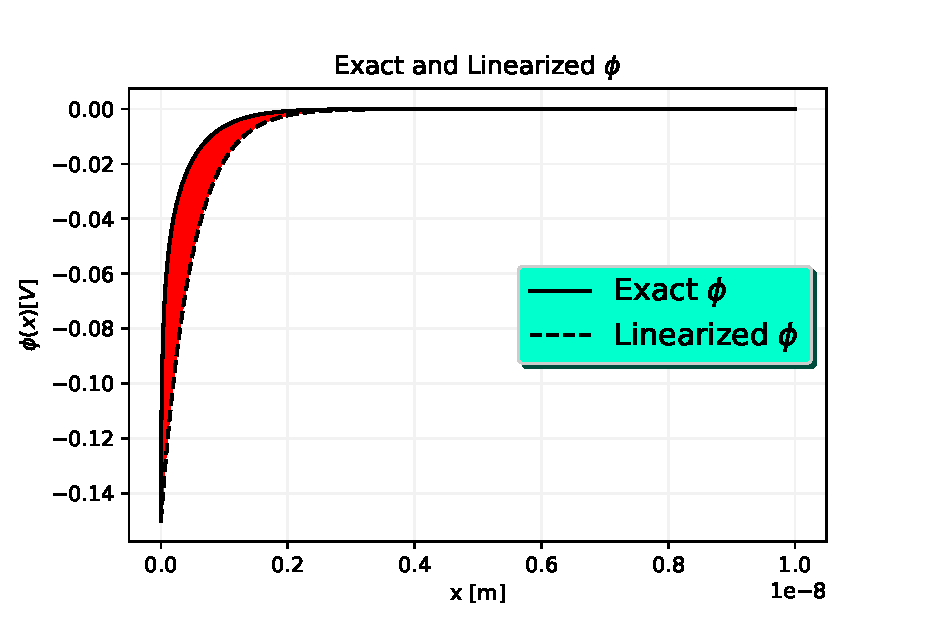
\includegraphics[width = 0.6\linewidth]{comparison-phi.eps}
 \caption{Comparison of the linearized PB solution with the analytical solution. The region in red is the error committed in this approximation}
\end{figure}

This results gives a good physical sense of how the potential should look like in a context of electrolyte solutions at equilibrium. We are interested in the dynamics of the system, though, so it makes sense to try to incorporate the current into Eq. \ref{eq:system}. In the next section we shall incorporate the current flowing through the interface as a border condition of Eq. \ref{eq:system}.

\section{Steady State Solution To The Diffusion-Reaction Problem}

In what follows, we shall assume that the system presents concentration gradients and
potential gradients along a single dimension $x$. This is equivalent to considering the interface infinitely large. Therefore, $\mathbf{N}_{+} = \hat{x}N_{+}$ and $\mathbf{N}_{-} = \hat{x}N_{-}$. 

In the steady state solution the concentration distribution of each electrolyte throughout the system should not change in time, thus

$$\frac{\partial C_+}{\partial t} = \frac{\partial C_-}{\partial t} = 0$$

This yields the following results

$$\nabla\cdot \mathbf{N}_+ = \frac{\partial N_{+}}{\partial x}=0$$
$$\nabla \cdot \mathbf{N}_- = \frac{\partial N_{-}}{\partial x}=0$$

Therefore, we have

$$N_+ = A_1$$
$$N_- = A_2$$

where $A_1$ and $A_2$ are constants determined by border conditions. Since the anion does not interact with the interface, we get after Eq.(\ref{eq_bc1})
$N_- = 0$. On the other hand, the flux due to the cation reaction with the interface ($Cu^{+2}\rightarrow Cu^{0}$) gives the boundary condition for $N_+$,

$$N_+ = \frac{I_0}{Az_+F}$$

The complete system of equations to be solved is

$$N_-(x) = 0$$

$$N_+(x) = \frac{I_0}{Aze}$$

\begin{figure}[h!]
\centering
	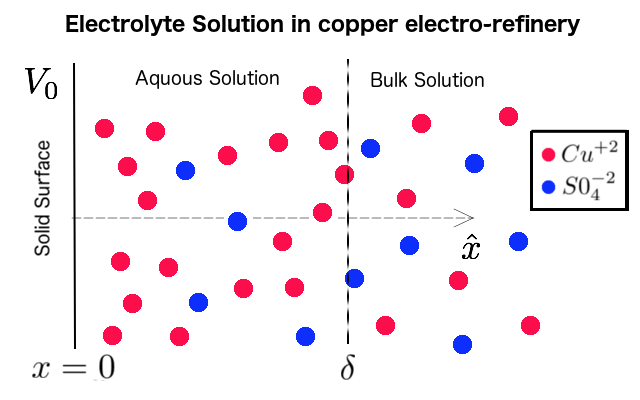
\includegraphics[width=0.5\textwidth]{geometry.png}
	\caption{Geometry of the problem. $x<\delta$ is the region of laminar. $x>\delta$ is the bulk of the solution. This image is for a value of $V_0<0$, such that the positive electrolytes distribute closer to the surface.}
\label{fig:geometry}
\end{figure}


According to Fig. \ref{fig:geometry}, for an interface area large compared to the laminar flux region we get the following equations 

\begin{eqnarray}\label{eq:system}
\frac{\partial C_+}{\partial x}-\frac{z F}{RT}C_+\frac{\partial \phi}{\partial x} &=& -\frac{I_0}{D_+Az_+ F}\label{eq:eq1} \\
\frac{\partial C_-}{\partial x}+\frac{z F}{RT}C_-\frac{\partial \phi}{\partial x} &=& 0 \label{eq:eq2}\\
\frac{\partial^2 \phi}{\partial x^2} &=& -\frac{1}{\epsilon} \sum_{s=\pm}z_s F C_s(x)\label{eq:eq3}
\end{eqnarray}

where A is the area of the interface electrode. 

To solve this system of partial differential equations, we will expand the concentration and the potential as a series in powers of $r = \frac{I_0}{D_+Az_+ F}$. We have

\begin{eqnarray}
C_s(x) = \sum_{n=0}^{\infty}r^n C_s^{(n)}(x)\\
\phi(x) = \sum_{n=0}^{\infty}r^n \phi^{(n)}(x)
\end{eqnarray}

Truncating the series at first order in $r$, we obtain the following system of equations to order zero in the current
\begin{eqnarray}
\frac{\partial C^{(0)}_+}{\partial x}-\frac{zF}{RT}C^{(0)}_+(x)\frac{\partial \phi^{(0)}}{\partial x} &=& 0\\
\label{eq:concentration-diff-zero1}
\frac{\partial C^{(0)}_-}{\partial x}+\frac{zF}{RT}C^{(0)}_-(x)\frac{\partial \phi^{(0)}}{\partial x}&=& 0\\
\label{eq:concentration-diff-zero2}
\frac{\partial^2  \phi^{(0)}}{\partial x^2} &=& -\frac{1}{\epsilon}\sum_{s= \pm} szF C^{(0)}_{s}(x)
\label{eq:concentration-diff-zero3}
\end{eqnarray}

and to first order in the current

\begin{eqnarray}
\frac{\partial C^{(1)}_+}{\partial x}-\frac{zF}{RT}\qty{C^{(1)}_+(x)\frac{\partial \phi^{(0)}}{\partial x}+C^{(0)}_+(x)\frac{\partial \phi^{(1)}}{\partial x}} &=& -1,\\
\label{eq:concentration-diff-first1}
\frac{\partial C^{(1)}_-}{\partial x}+\frac{zF}{RT}\qty{C^{(1)}_-(x)\frac{\partial \phi^{(0)}}{\partial x}+C^{(0)}_-(x)\frac{\partial \phi^{(1)}}{\partial x}}&=& 0,\\
\label{eq:concentration-diff-first2}
\frac{\partial^2  \phi^{(1)}}{\partial x^2} &=& -\frac{1}{\epsilon}\sum_{s= \pm} szF C^{(1)}_{s}(x).
\label{eq:concentration-diff-first3}
\end{eqnarray}




















\newpage

\section{Zero order solution to Poisson's equation for the electrolyte solution}
\label{sec:zeroorderphi}

We want to work with the dimensionless potential 

$$\Phi(x) = \frac{zF}{RT}\phi(x).$$

The zero order system can thus be written as

\begin{eqnarray}
\label{eq:zero-order}
C^{(0)}_+(x)'-C^{(0)}_+(x)\Phi^{(0)}(x)' &=& 0\\
 C^{(0)}_-(x)'+C^{(0)}_-(x)\Phi^{(0)}(x)'&=& 0\\
\Phi^{(0)}(x) ''&=& -\frac{(zF)^2}{RT\epsilon} (C^{(0)}_{+}(x)-C^{(0)}_{-}(x))
\end{eqnarray}



In this section we will solve equations \ref{eq:concentration-diff-first1} and \ref{eq:concentration-diff-first2}. 

From Eq. \ref{eq:zero-order},

$$\frac{\partial C^{(0)}_s}{\partial x}-sC^{(0)}_s\Phi^{(0)}(x)= 0$$

which yields

$$\int_{C_{b,s}}^{C^{(0)}_s(x)} \frac{dC^{(0)}_s}{C^{(0)}_s}=s\int_{\phi_b}^{\phi^{(0)}} d\Phi^{(0)}$$

where $\Phi_b = \Phi(\delta)$ is the potential at the bulk, which we will consider as the reference zero, $\phi_b = 0$. $C_{b,s}$ is the bulk concentration of each species in solution.

$$C^{(0)}_s(x)=C_{b,s}e^{s\Phi^{(0)}(x)}$$

Notice that 
\begin{equation}
C^{(0)}_s(\delta) = C_{b,s}e^{\frac{zF}{RT}\phi_b}=C_{b,s}.
\label{eq:zero-order-sol-c}
\end{equation}

Consider the bulk values of the concentration, $C_{s,b}$. In the bulk, the solution should be electrically neutral due to conservation of charge. Therefore, for a two electrolyte salt at the bulk

\begin{equation}
\label{eq:electroneutrality}
\sum_{s=\pm} C_{s,b} sz F = 0
\end{equation}


where $z$ is the valence of the electrolytes and $s = \pm$ is the sign of the charge of the electrolyte. $F = eN_A$ is the Faraday constant. From \ref{eq:electroneutrality} we get,

\begin{eqnarray}\nonumber
C_{b,+}Fz-C_{b,-}Fz=0\\
\rightarrow \frac{C_{b,+}}{C_{b,-}}=1
\label{eq:electroneutrality2}
\end{eqnarray}

$$C_{b,+}Fz-C_{b,-}Fz=0$$
$$\rightarrow \frac{C_{b,+}}{C_{b,-}}=1$$

In the case of a symmetric salt, $q_s=-q_{-s}$ (since in our notation $s=\pm$). Poisson's equation can be written (to zero order in the current) as

\begin{equation}
\label{eq:poisson1}
\frac{\partial^2 \Phi^{(0)}}{\partial x^2} = -\frac{zF}{\epsilon} \left(C_{b,+}e^{\Phi^{(0)}(x)}-C_{b,-}e^{-\Phi^{(0)}(x)}\right)
\end{equation}

where $z=|z_-|=|z_+|$. From equations \ref{eq:zero-order-sol-c}  and \ref{eq:electroneutrality2} we have $C_{b,+}=C_{b,+} = C_b$. Equation \ref{eq:poisson1} can be written in terms of the hyperbolic sine,

\begin{equation}
\label{eq:poisson2}
\frac{\partial^2 \Phi^{(0)}}{\partial x^2} = 2\frac{(zF)^2C_b}{RT\epsilon}\sinh{\left(\Phi^{(0)}(x)\right)}
\end{equation}

We define the quantity  

$$\kappa^2  = \frac{(zF)^2C_b}{RT\epsilon}$$

\begin{equation}
\frac{\partial^2 \Phi^{(0)}}{\partial x^2} = 2\kappa \sinh{\left(\Phi^{(0)}(x)\right)}
\end{equation}

We want to change variables to the dimensionless quantity $\kappa x$,

$$x \rightarrow \xi = \kappa x$$
 $$d \xi  = \kappa d x $$
 
Thus, we write,

\begin{equation}
\Phi^{(0)}(\xi)''= 2\sinh{\left(\Phi^{(0)}(\xi)\right)}
\end{equation}

Multiplying by  $\Phi'^{(0)}$ and integrating the equation over the interval $[\xi, \delta]$ we get,
 
\begin{align}
\Phi^{(0)}(\kappa \delta)'^2  -\Phi^{(0)}(\xi)'^2   = 2(cosh(\phi(\kappa \delta))-cosh(\phi(\xi)))
\end{align}

The border condition for the potential yields, 

$$\Phi^{(0)}(\xi)' \rightarrow 0.$$

Therefore

\begin{align}
\Phi^{(0)}(\xi)'^2   &= 2(\cosh(\phi(\xi))-1),\\
&= 4sinh^2(\phi(\xi)), \\
\rightarrow \Phi^{(0)} &= \pm 2\sinh(\phi(\xi).
\label{eq:phiprime}
\end{align}


The border conditions for the potential are $\Phi^{(0)}(0) = \bar{V}_0<0$ and $\Phi^{(0)}(\kappa \delta) = 0$, the slope of $\Phi^{(0)}$ must be positive and decreasing. This yields the positive solution to equation \ref{eq:phiprime}
\begin{align}
\Phi^{(0)} &=  2\sqrt{\sinh(\phi(\xi))}.
\end{align}

This is a separable equation which can be integrated directly, yielding

\begin{align}
	\log\qty{\frac{1-e^{\Phi^{(0)}/2}}{1+e^{\Phi^{(0)}/2}}} = -\xi + C,
\end{align}

\begin{align}
	\rightarrow \frac{1-e^{\Phi^{(0)}/2}}{1+e^{\Phi^{(0)}/2}}= Ae^{-\xi}.
\end{align}

It can be found using the border condition $\Phi^{(0)}(0) = \bar{V}_0$

\begin{align}
A = \tanh\qty{{\bar{V}_0/4}}
\end{align}

Solving for $\Phi^{(0)}$,

\begin{align}
\Phi^{(0)}(\xi) =  2\log{\qty{\tanh\qty{\frac{\xi-\xi_0}{2}}}},
\label{eq:pot0}
\end{align}

where we have defined

$$.$$

The minus sign in the previous definition is due to the fact that $\bar{V}_0 < 0$ for our case.




\section{Charge Density At The Interface}

From equation \ref{eq:pot0} we can obtain the electric field, which in terms of $x$ has the form

\begin{align}
E(x) =  \frac{2\kappa}{\beta q} \csc\qty{\kappa(x-x_0)},
\label{eq:pot0}
\end{align}

where

\begin{align}
e^{\xi_0} = -\tanh\qty{\frac{\bar{V}_0}{4}}.
\label{eq:expz0}
\end{align}

From electrostatics we know that the border condition for the electric field at a conductors interface is
\begin{align}
	E(x)\big|_{interface} = \frac{\sigma}{\epsilon}.
\end{align}

We thus obtain the surface charge in terms of the voltage at the interface

\begin{align}
	\sigma = -\frac{2 \epsilon \kappa}{\beta q} \csc\qty{kz_0},
\end{align}

which using Eq. \ref{eq:expz0} can be written as

\begin{align}
	\sigma(V_0) = -\frac{2 \epsilon \kappa}{\beta q} \frac{\tanh\qty{\frac{q\beta V_0}{4}}}{\tanh\qty{\frac{q\beta V_0}{4}}-1}
\end{align}

This equation can be solved for $V_0$ in terms of the surface charge density $\sigma$

\begin{align}
	V_0 = \tanh^{-1}\qty{-\frac{8\epsilon\kappa}{(q \beta)^2 \sigma} \qty{1 \pm \frac{1}{2}\sqrt{1+\frac{\beta^2 q^2\sigma^2}{\epsilon^2\kappa^2}}}}
\end{align}


\begin{figure}[htbp!]
\centering
\begin{subfigure}{.4\textwidth}
  \centering
  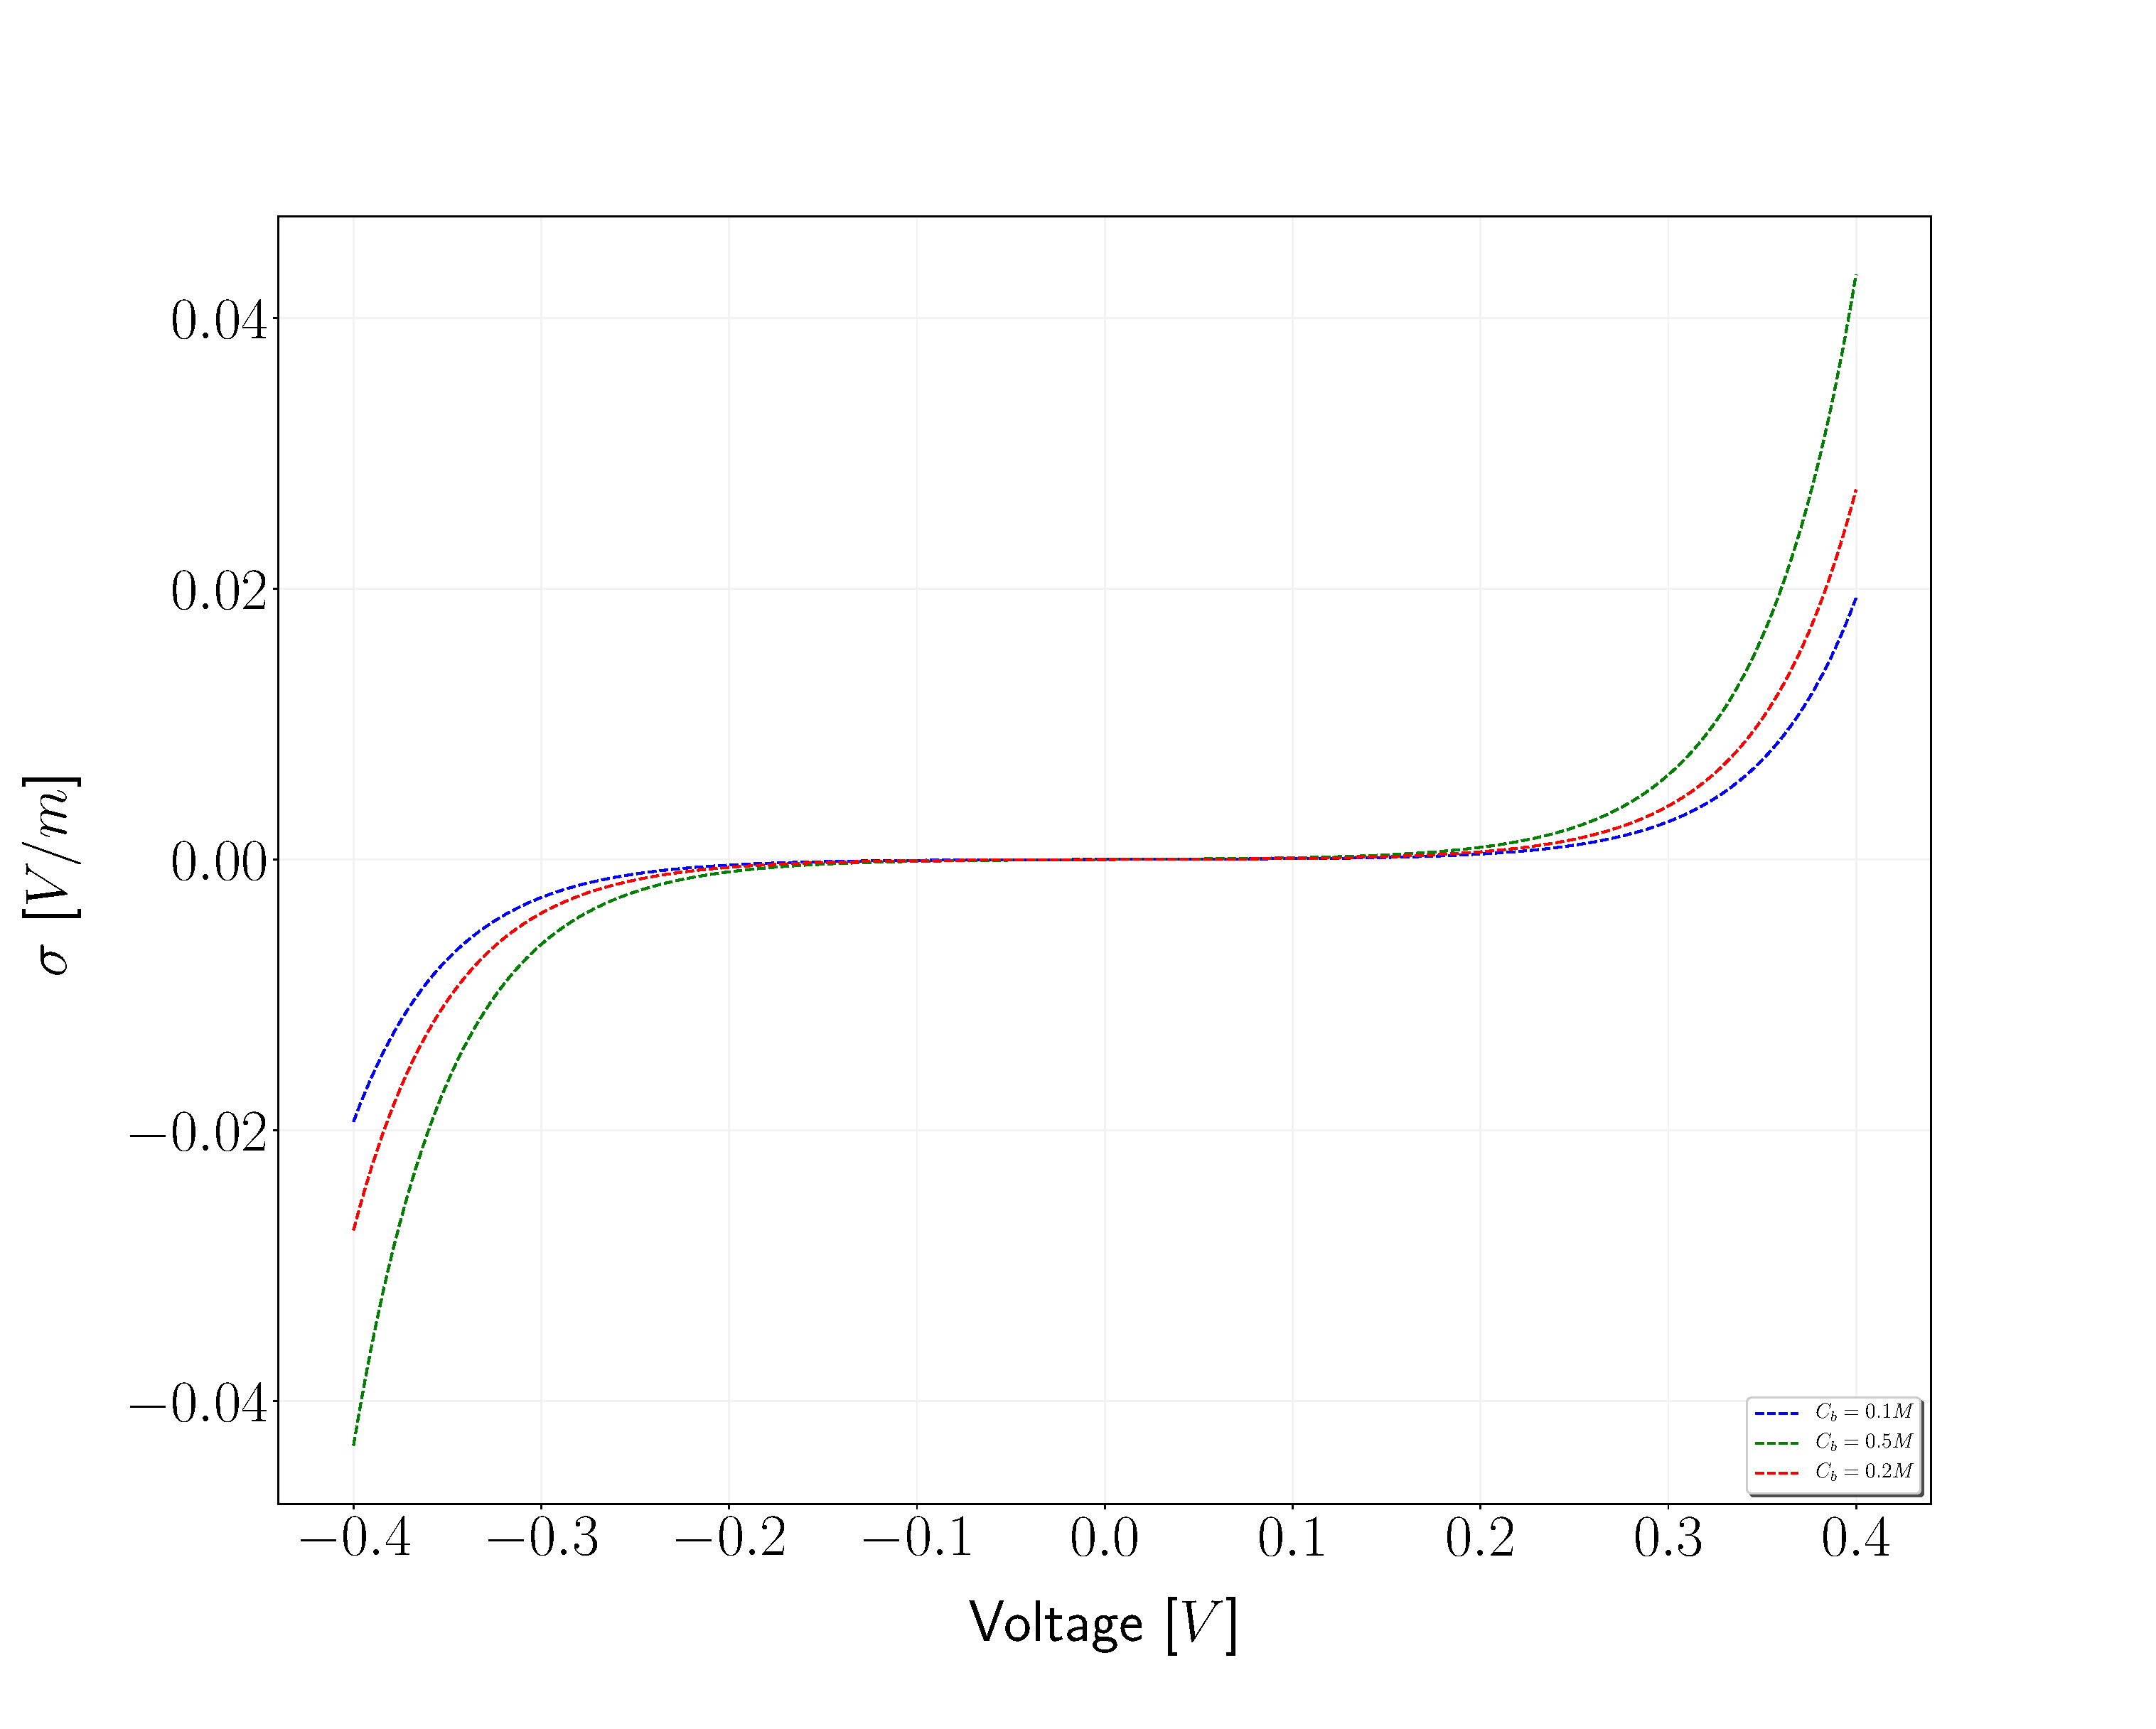
\includegraphics[width=\linewidth]{sigma-voltage.eps}
  \caption{}
  \label{fig:sub1}
\end{subfigure}%
\begin{subfigure}{.4\textwidth}
  \centering
  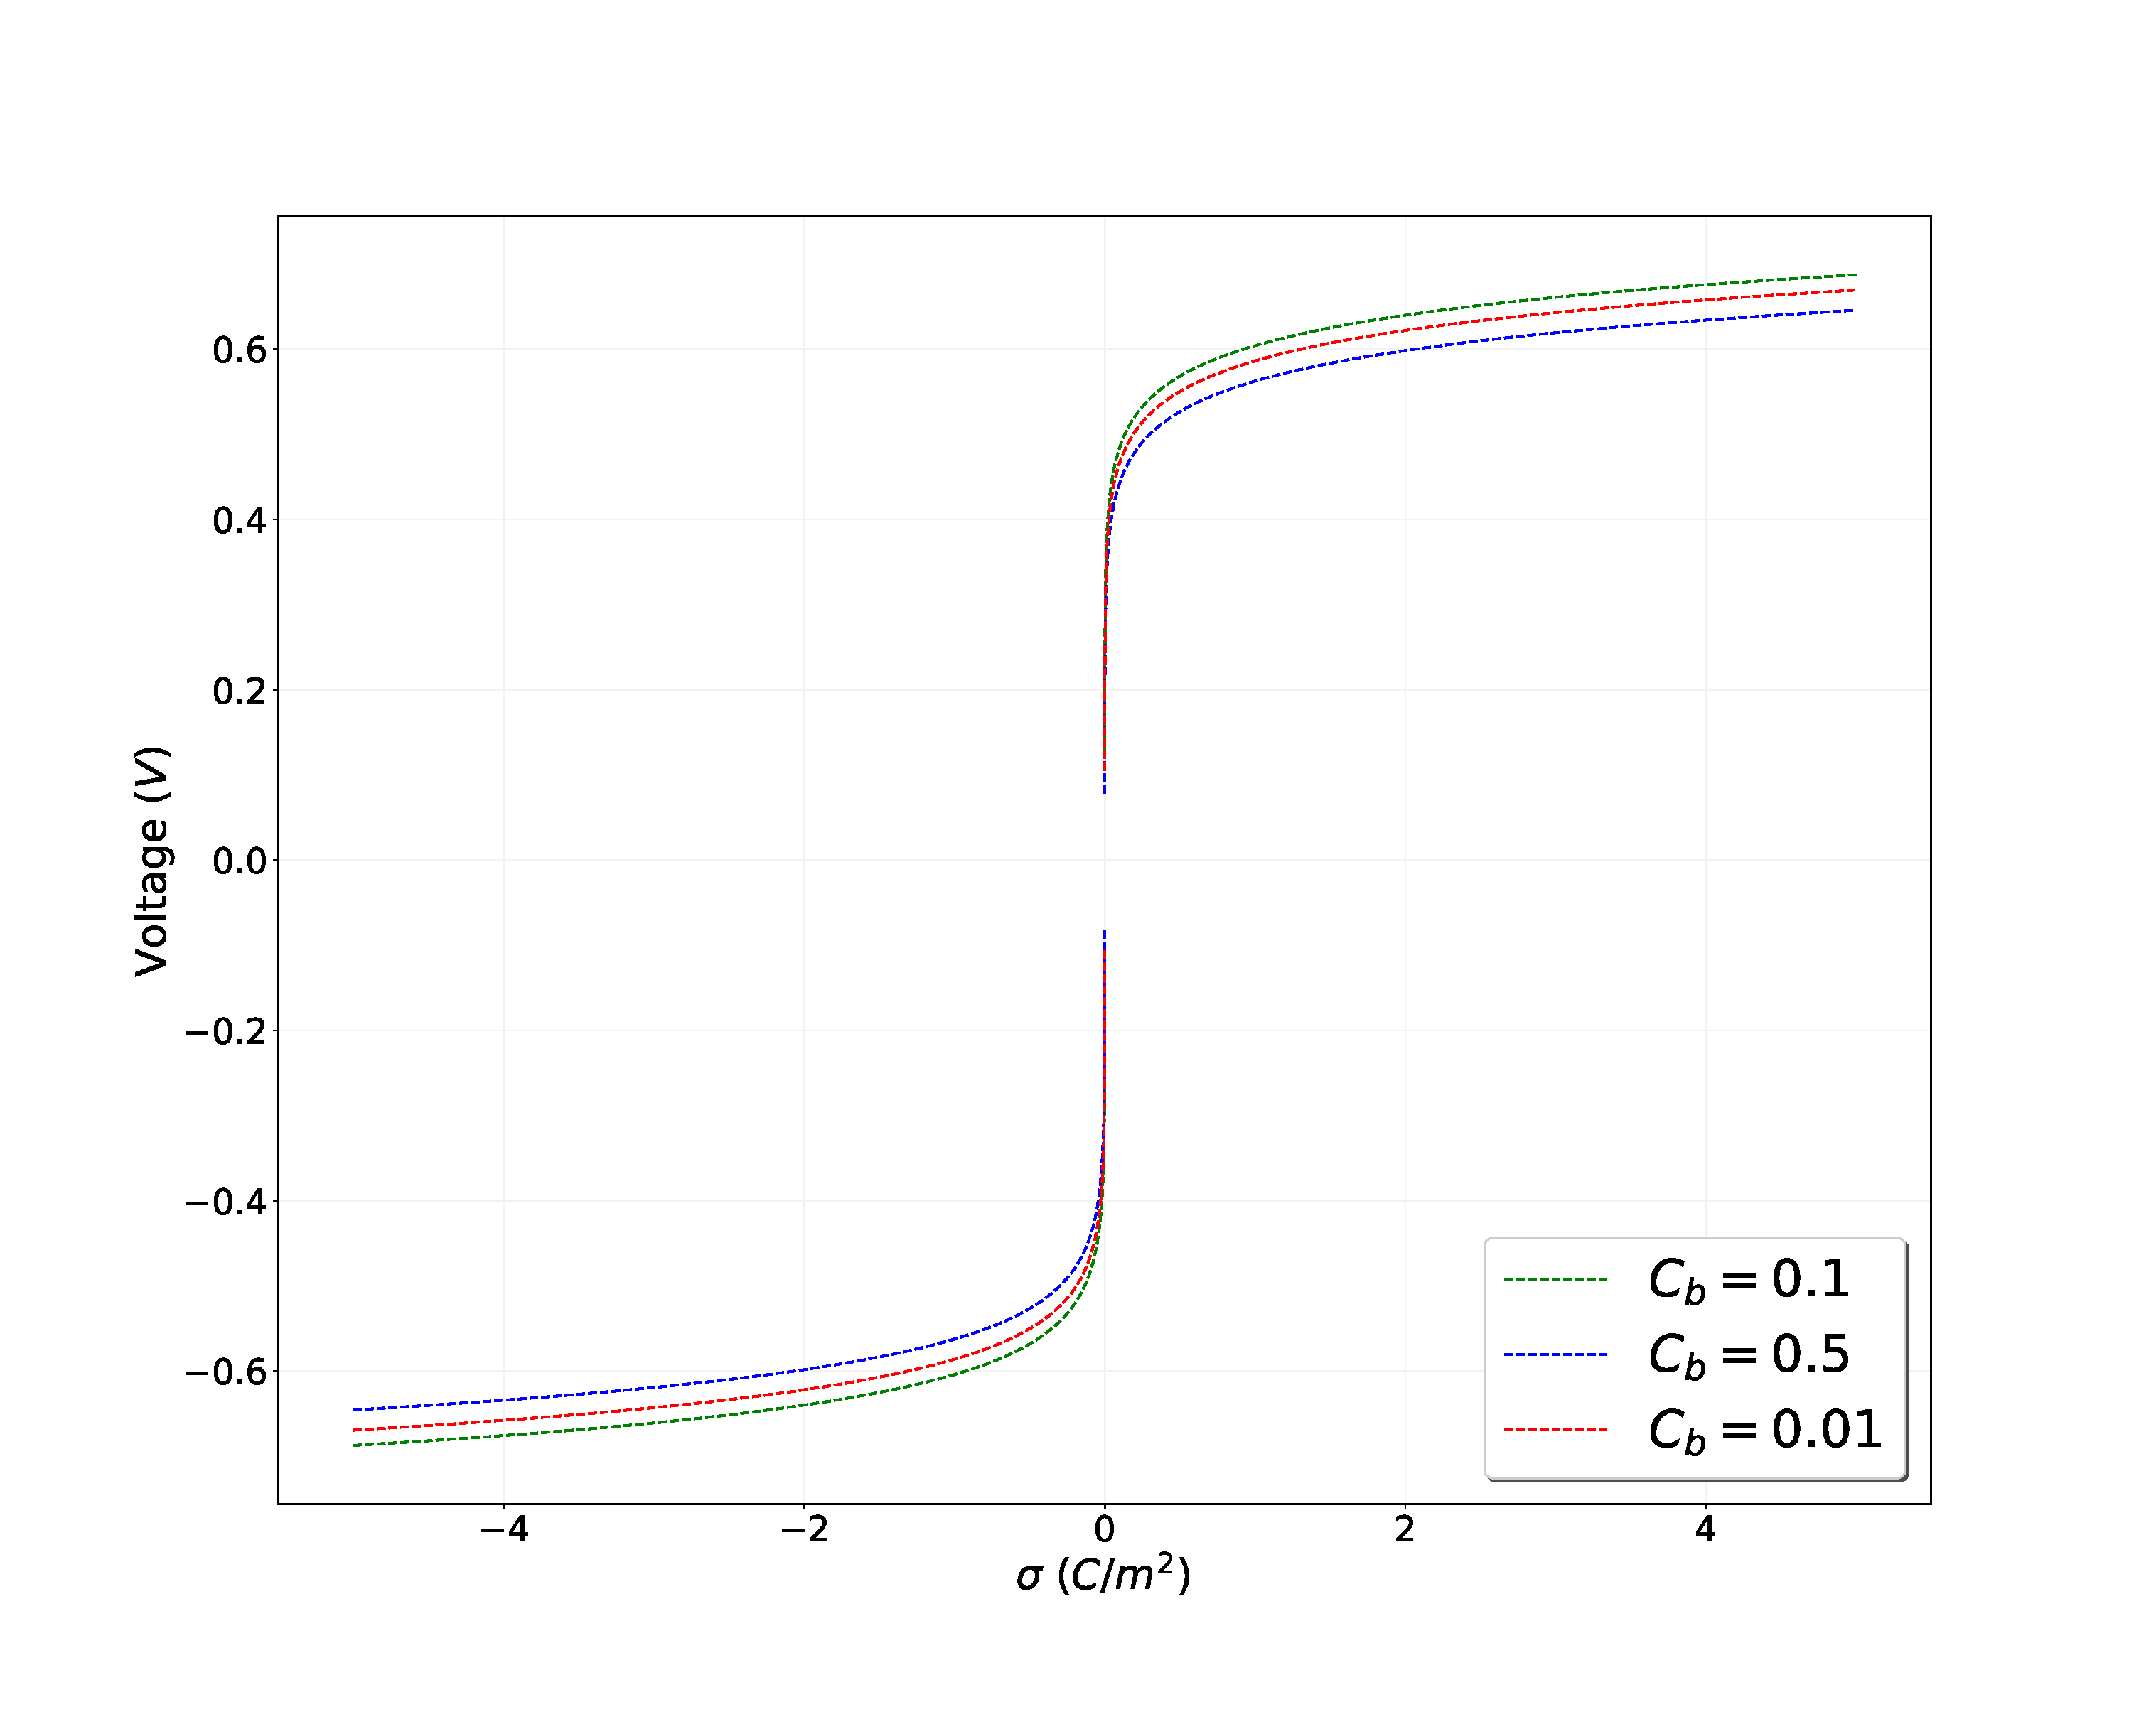
\includegraphics[width=\linewidth]{voltage-sigma.eps}
  \caption{}
  \label{fig:sub2}
\end{subfigure}
\caption{\textbf{(a)} Surface charge density in terms of the potential border condition. \textbf{(b)} Inverse of (a)}
\label{fig:test}
\end{figure}

\begin{figure}[htbp!]
\centering
\begin{subfigure}{.4\textwidth}
  \centering
  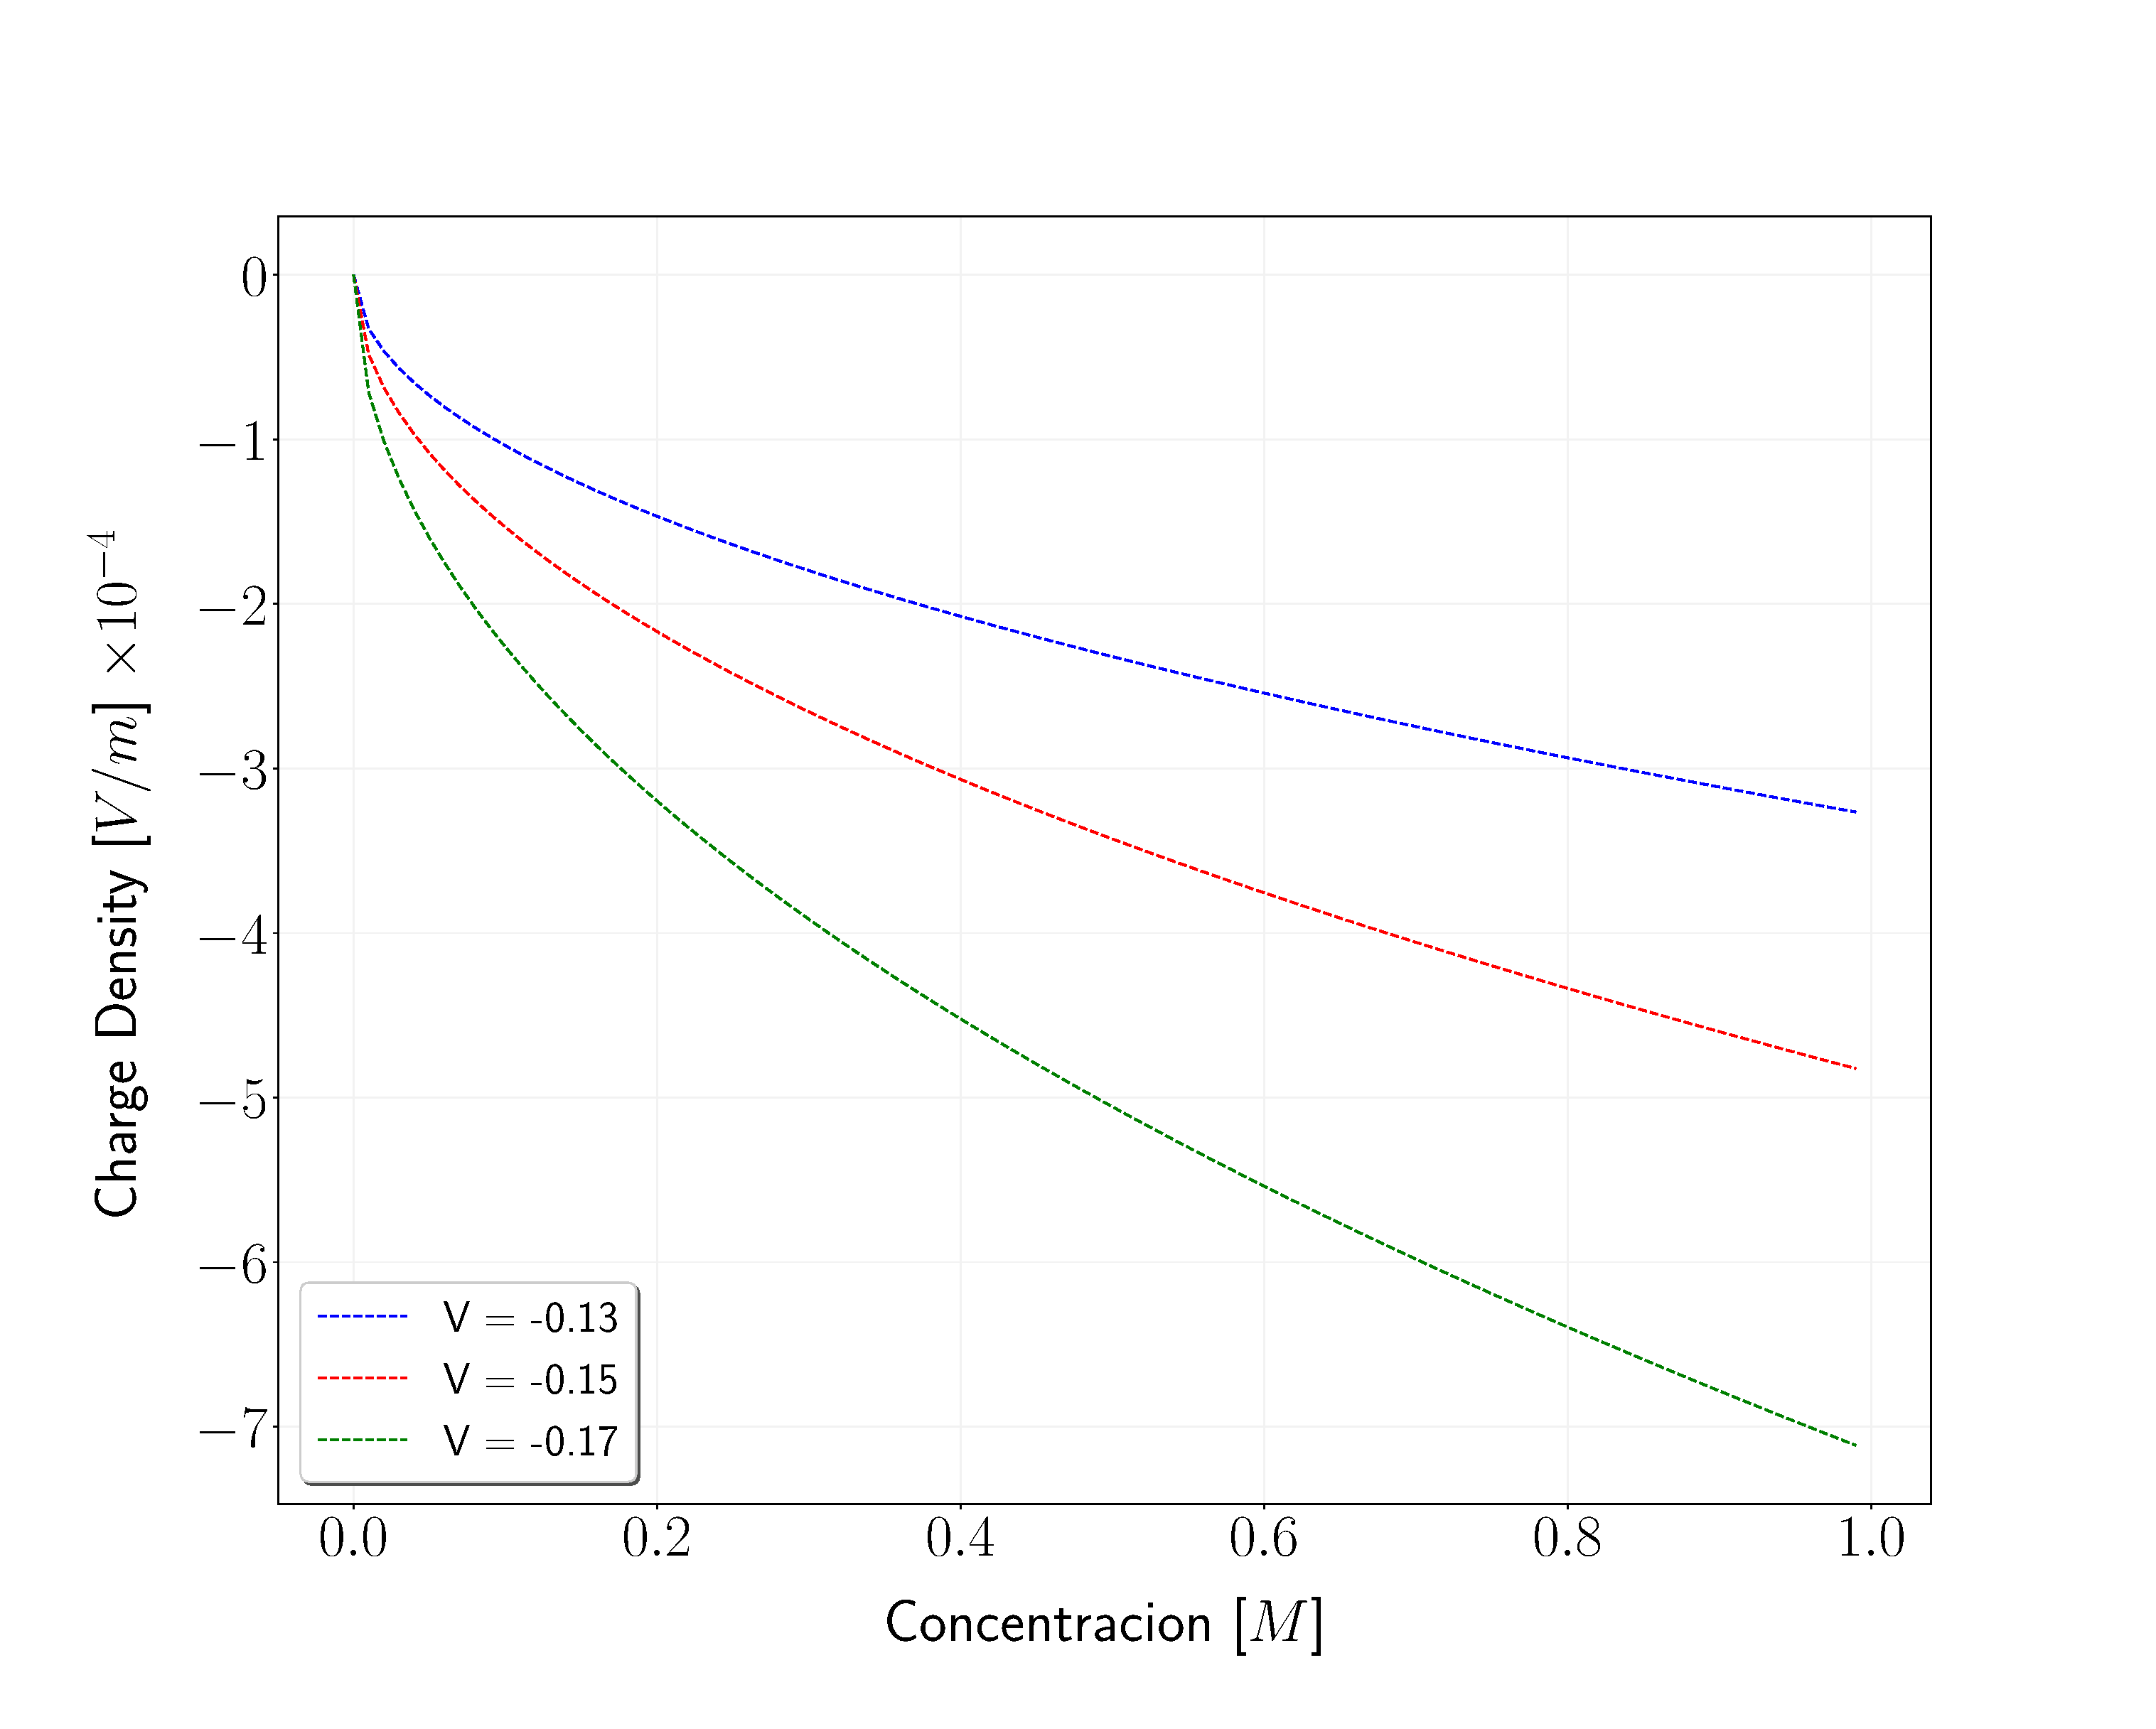
\includegraphics[width=\linewidth]{sigma-concentration.eps}
  \caption{}
  \label{fig:sub1}
\end{subfigure}%
\begin{subfigure}{.4\textwidth}
  \centering
  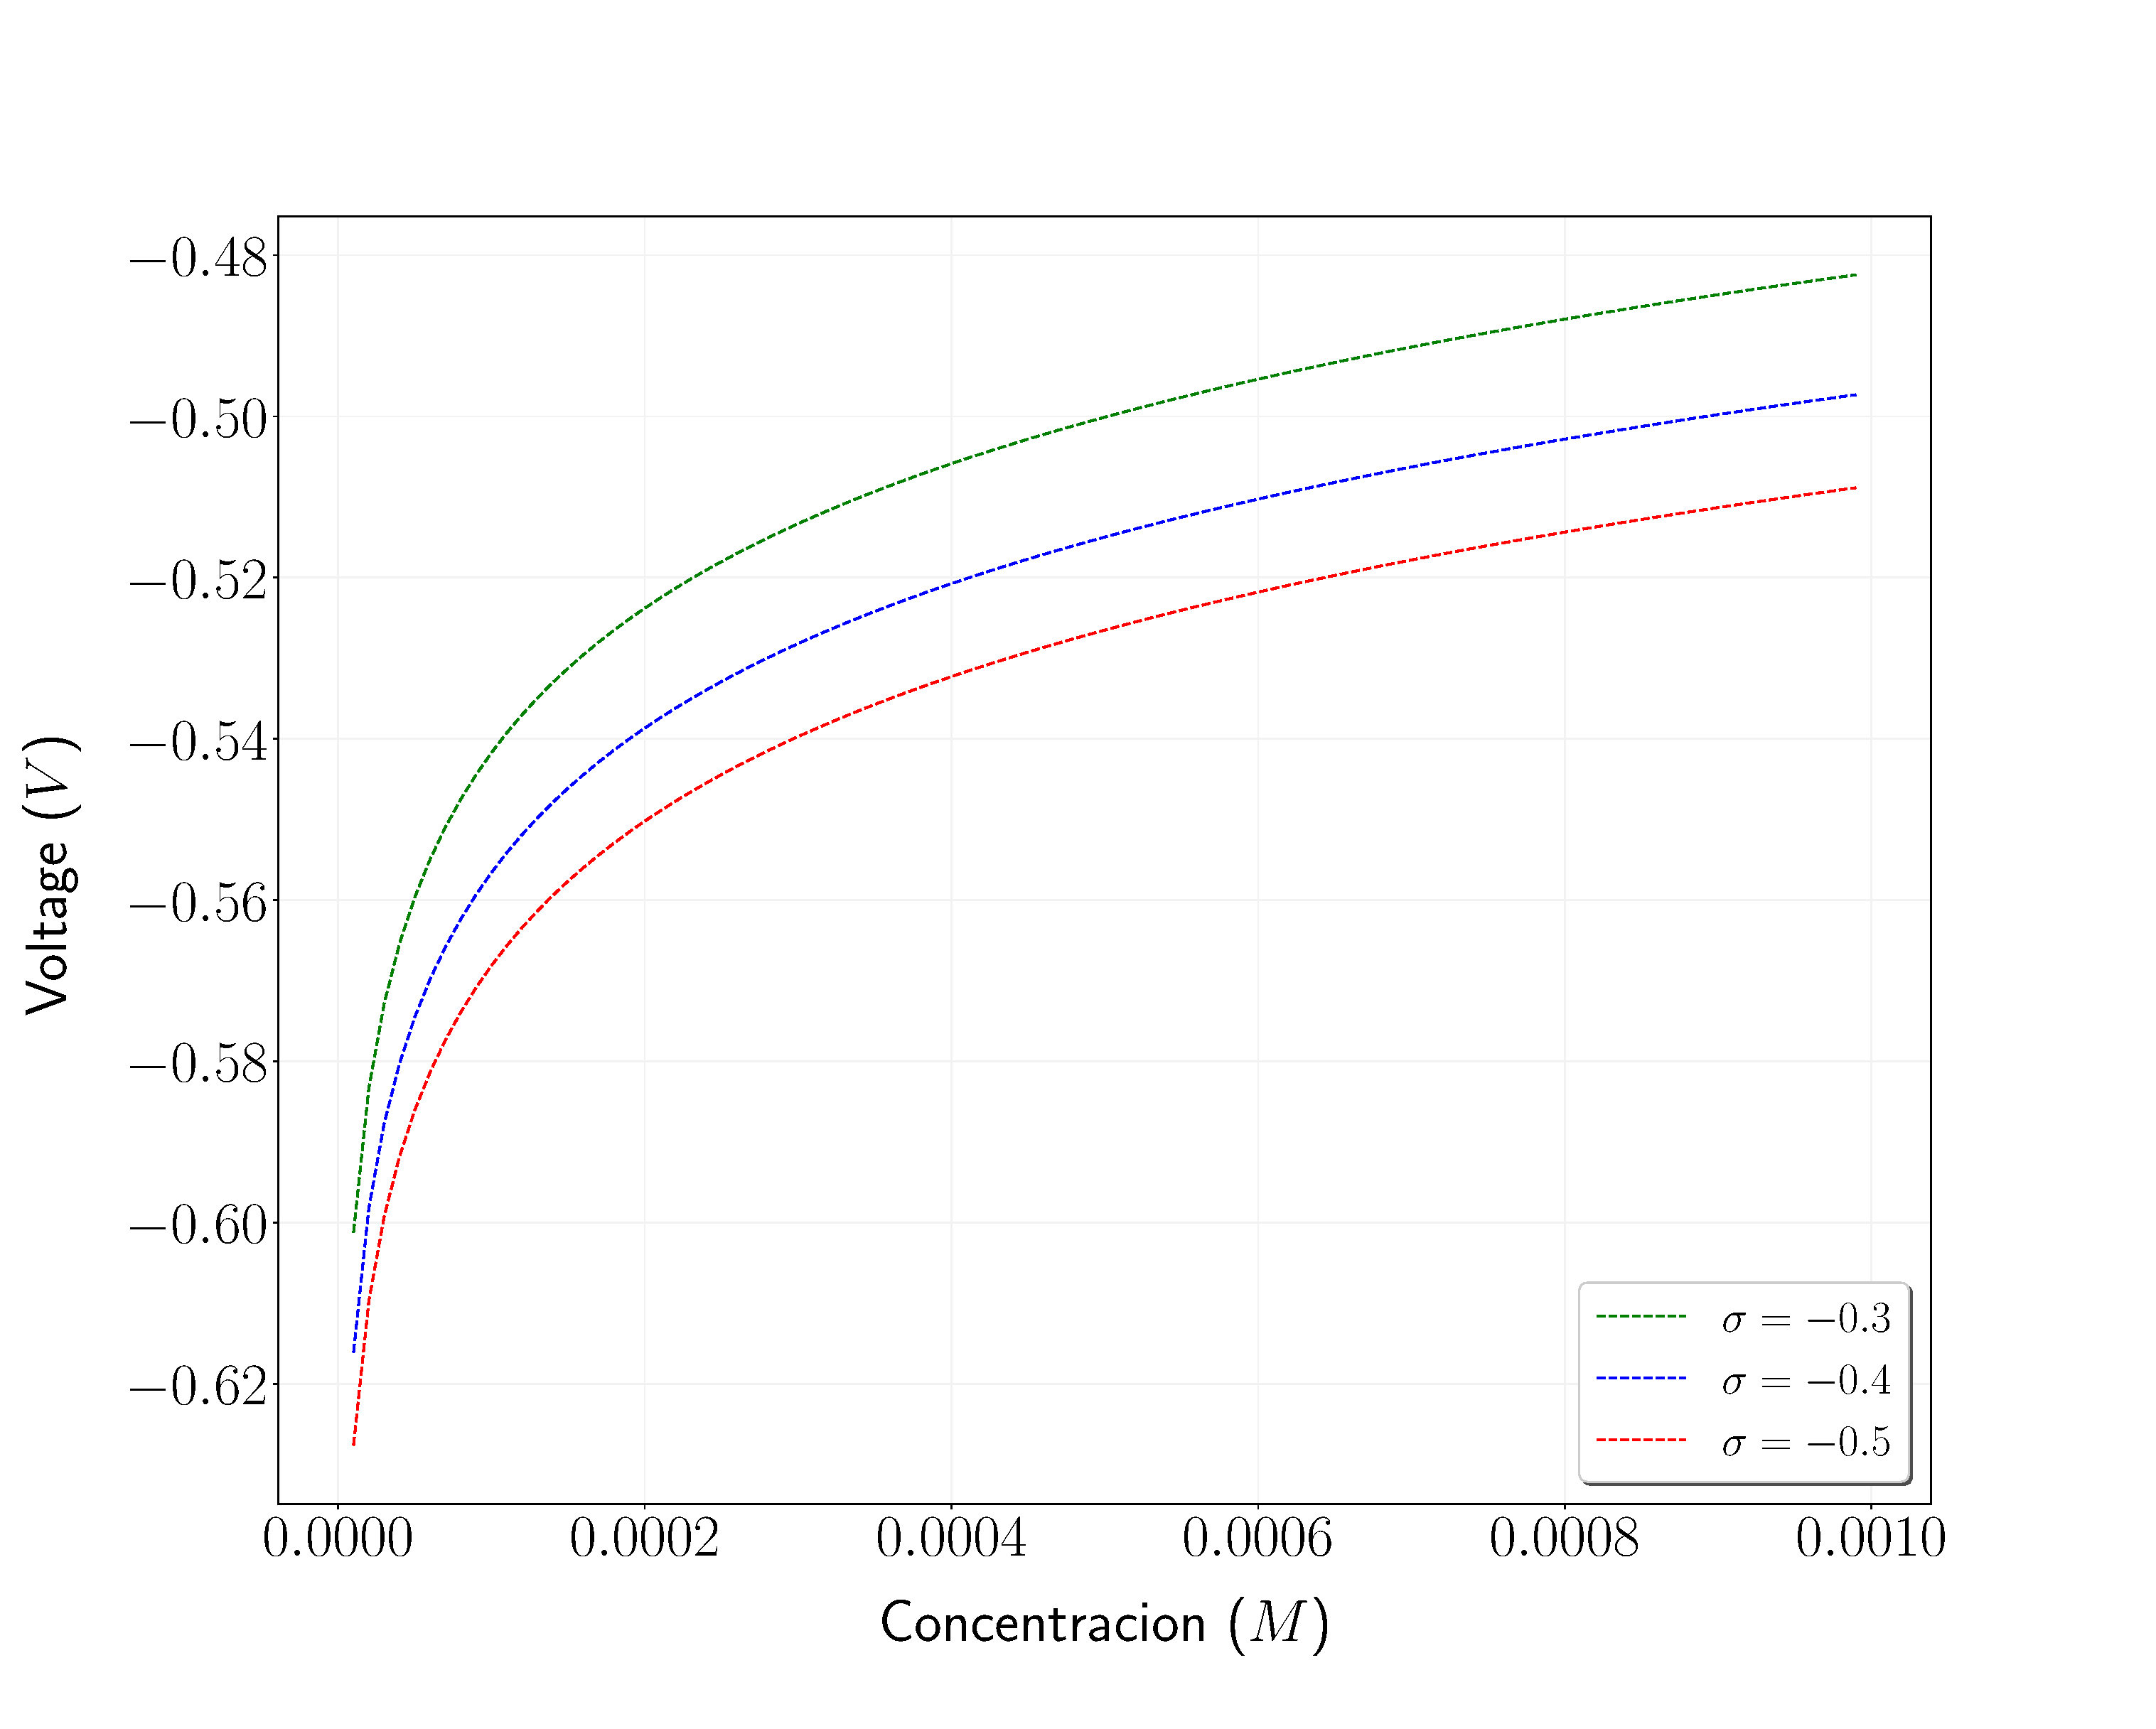
\includegraphics[width=\linewidth]{voltage-concentration.eps}
  \caption{}
  \label{fig:sub2}
\end{subfigure}
\caption{\textbf{(a)} Surface charge density in terms of the bulk concentration. \textbf{(b)} Voltage at the interface in terms of the bulk concentration (a)}
\label{fig:test}
\end{figure}




\section{Solution to the concentration at first order in the current $I_0$}


Now we solve Equation \ref{eq:system} at first order in the current $I_0$. From Eq. \ref{eq:concentration-diff-first2}, we consider the term proportional to $\frac{\partial \phi^{(1)}}{\partial x}$ such that

\begin{equation}
\bigg|\frac{\partial \phi^{(1)}}{\partial x}\bigg| << \frac{\kappa V_0}{r},
\label{eq:approx}
\end{equation}

since the gradient of the correction to the potential should be negligible compared to the gradient of the zero order contribution. This will be shown later in a numerical analysis. With this approximation, the system to first order in $r$ becomes

\begin{eqnarray}
\frac{\partial C^{(1)}_+}{\partial \xi}-C^{(1)}_+(\xi)\frac{\partial \Phi^{(0)}}{\partial \xi} &=& -\frac{1}{\kappa} \\
\label{eq:concentration-diff-first4}
\frac{\partial C^{(1)}_-}{\partial \xi}+C^{(1)}_-(\xi)\frac{\partial \Phi^{(0)}}{\partial \xi} &=& 0 \\
\label{eq:concentration-diff-first5}
\frac{\partial^2  \phi^{(1)}}{\partial \xi^2} &=& -(C^{(1)}_{+}(\xi)-C^{(1)}_{-}(\xi))
\label{eq:concentration-diff-first6}
\end{eqnarray}


In Eq. \ref{eq:concentration-diff-first4}, we obtain

$$\frac{\partial C^{(1)}_+}{\partial \xi}-C^{(1)}_+\frac{\partial \Phi^{(0)}}{\partial \xi} = -\frac{1}{\kappa}$$

Using an integrating factor of the form
$$\mu(\xi)=e^{-\int_{\kappa\delta}^\xi \frac{zF}{RT}\frac{d\phi^{(0)}}{d\xi'}d\xi'}=e^{- (\Phi^{(0)}(\xi)-\phi_b)} = e^{-\Phi^{(0)}(\xi)}$$

We can write \ref{eq:concentration-diff-first4}  as

$$\frac{d}{d\xi}\left(C^{(1)}_+(\xi)\mu(\xi) \right)=-\frac{\mu(\xi)}{\kappa},$$

where $z=|z_\pm|$. Integrating over $x$ and considering that $C^{(1)}_+(\xi)\mu(\xi)\big|_{\xi \rightarrow \infty} = C^{(1)}_{+,b} = 0$ due to border conditions, we get

$$C^{(1)}_+(\xi) =\frac{1}{\kappa\mu(\xi)}\int_{0}^{\xi}\mu(\xi')d\xi'$$

Eq. \ref{eq:concentration-diff-first5} can be integrated by separation of variables, and the solution is 

$$C^{(1)}_-(\xi) = C^{(1)}_{b,-}e^{\phi^{(0)}(\xi)}.$$

Since our border condition yields $ C^{(1)}_{b,-} = 0$, the contribution to first order of the negative ion concentration is zero. 

Computing the integral, we find to first order in the current the following solutions for the concentrations.

\begin{eqnarray}
C^{(1)}_+(\xi) &=& -\frac{1}{\kappa} \qty{\xi_\delta-\xi-\frac{2}{\gamma}}\tanh^2\qty{\frac{\xi-\xi_0}{2}}+2\tanh\qty{\frac{\xi-\xi_0}{2}}\\
C^{(1)}_-(\xi) &=& 0
\label{eq:firstordersol}
\end{eqnarray}



\section{Potential to first order in the current}

Now we need to solve Eq. \ref{eq:concentration-diff-first6}
\begin{eqnarray}
\frac{\partial^2  \Phi^{(1)}}{\partial \xi^2} &=& -(C^{(1)}_{+}(\xi)-C^{(1)}_{-}(\xi)).
\end{eqnarray}

Expanding, we have 

\begin{eqnarray}\nonumber
\frac{\partial^2  \Phi^{(1)}}{\partial \xi^2} &=& -C^{(1)}_{+}(\xi)\\
&=& -\frac{1}{\kappa} \qty{\xi_\delta-\xi-\frac{2}{\gamma}}\tanh^2\qty{\frac{\xi-\xi_0}{2}}+2\tanh\qty{\frac{\xi-\xi_0}{2}}
\end{eqnarray}


Integrating twice and using the fact that $\Psi'^{(1)} = 0$, $\Psi^{(1)} = 0$ we obtain

\begin{eqnarray}
\Phi'^{(1)}(\xi) = \frac{1}{\kappa} \qty{A + B\xi + C\xi^2 + D \tanh{\frac{\xi-\xi_0}{2}}+E\xi\tanh{\frac{\xi-\xi_0}{2}}} 
\end{eqnarray}


And 

\begin{eqnarray}
\Phi^{(1)}(\xi) = -\frac{1}{\kappa} (A(\xi_\delta - \xi) + \frac{B}{2}(\xi_\delta^2-\xi^2) + \frac{C}{3}(\xi_\delta^3 - \xi^3) + \\
D\log\bigg|\frac{\cosh{\frac{\xi_\delta-\xi}{2}}}{\cosh{\frac{\xi-\xi}{2}}}\bigg| + E \qty{\xi_\delta\log|\cosh\qty{\frac{\xi_\delta-\xi_0}{2}}-\xi\log|\cosh\qty{\frac{\xi-\xi_0}{2}}}-EI_\delta(\xi)
\end{eqnarray}


where

\begin{eqnarray*}
	A = 2\gamma\xi_\delta - \frac{2\xi_\delta}{\gamma} - 2 \gamma - \frac{\xi_\delta^2}{2},\\
	B = -\qty{\xi_\delta -\frac{2}{\gamma}},\\
	C = \frac{3}{2}\\
	D = -2 \qty{\xi_\delta - \frac{2}{\gamma}},\\
	E = 2,\\
	\gamma = \tanh\qty{\frac{\xi_0}{2}},
\end{eqnarray*}

and

\begin{align}
	I_\delta(\xi) = \int_\xi^{\xi_\delta} \log\bigg|\cosh\qty{\frac{\xi-\xi_0}{2}}\bigg| d\xi.
\end{align}




This integral must be evaluated numerically for each value of $\xi$. In order to do this, we use the Simpson Rule. Fig. \ref{fig:analytic-results} shows the potential to first order in the current alongside with the zero order potential. 


\begin{figure}[h!]
 \centering
 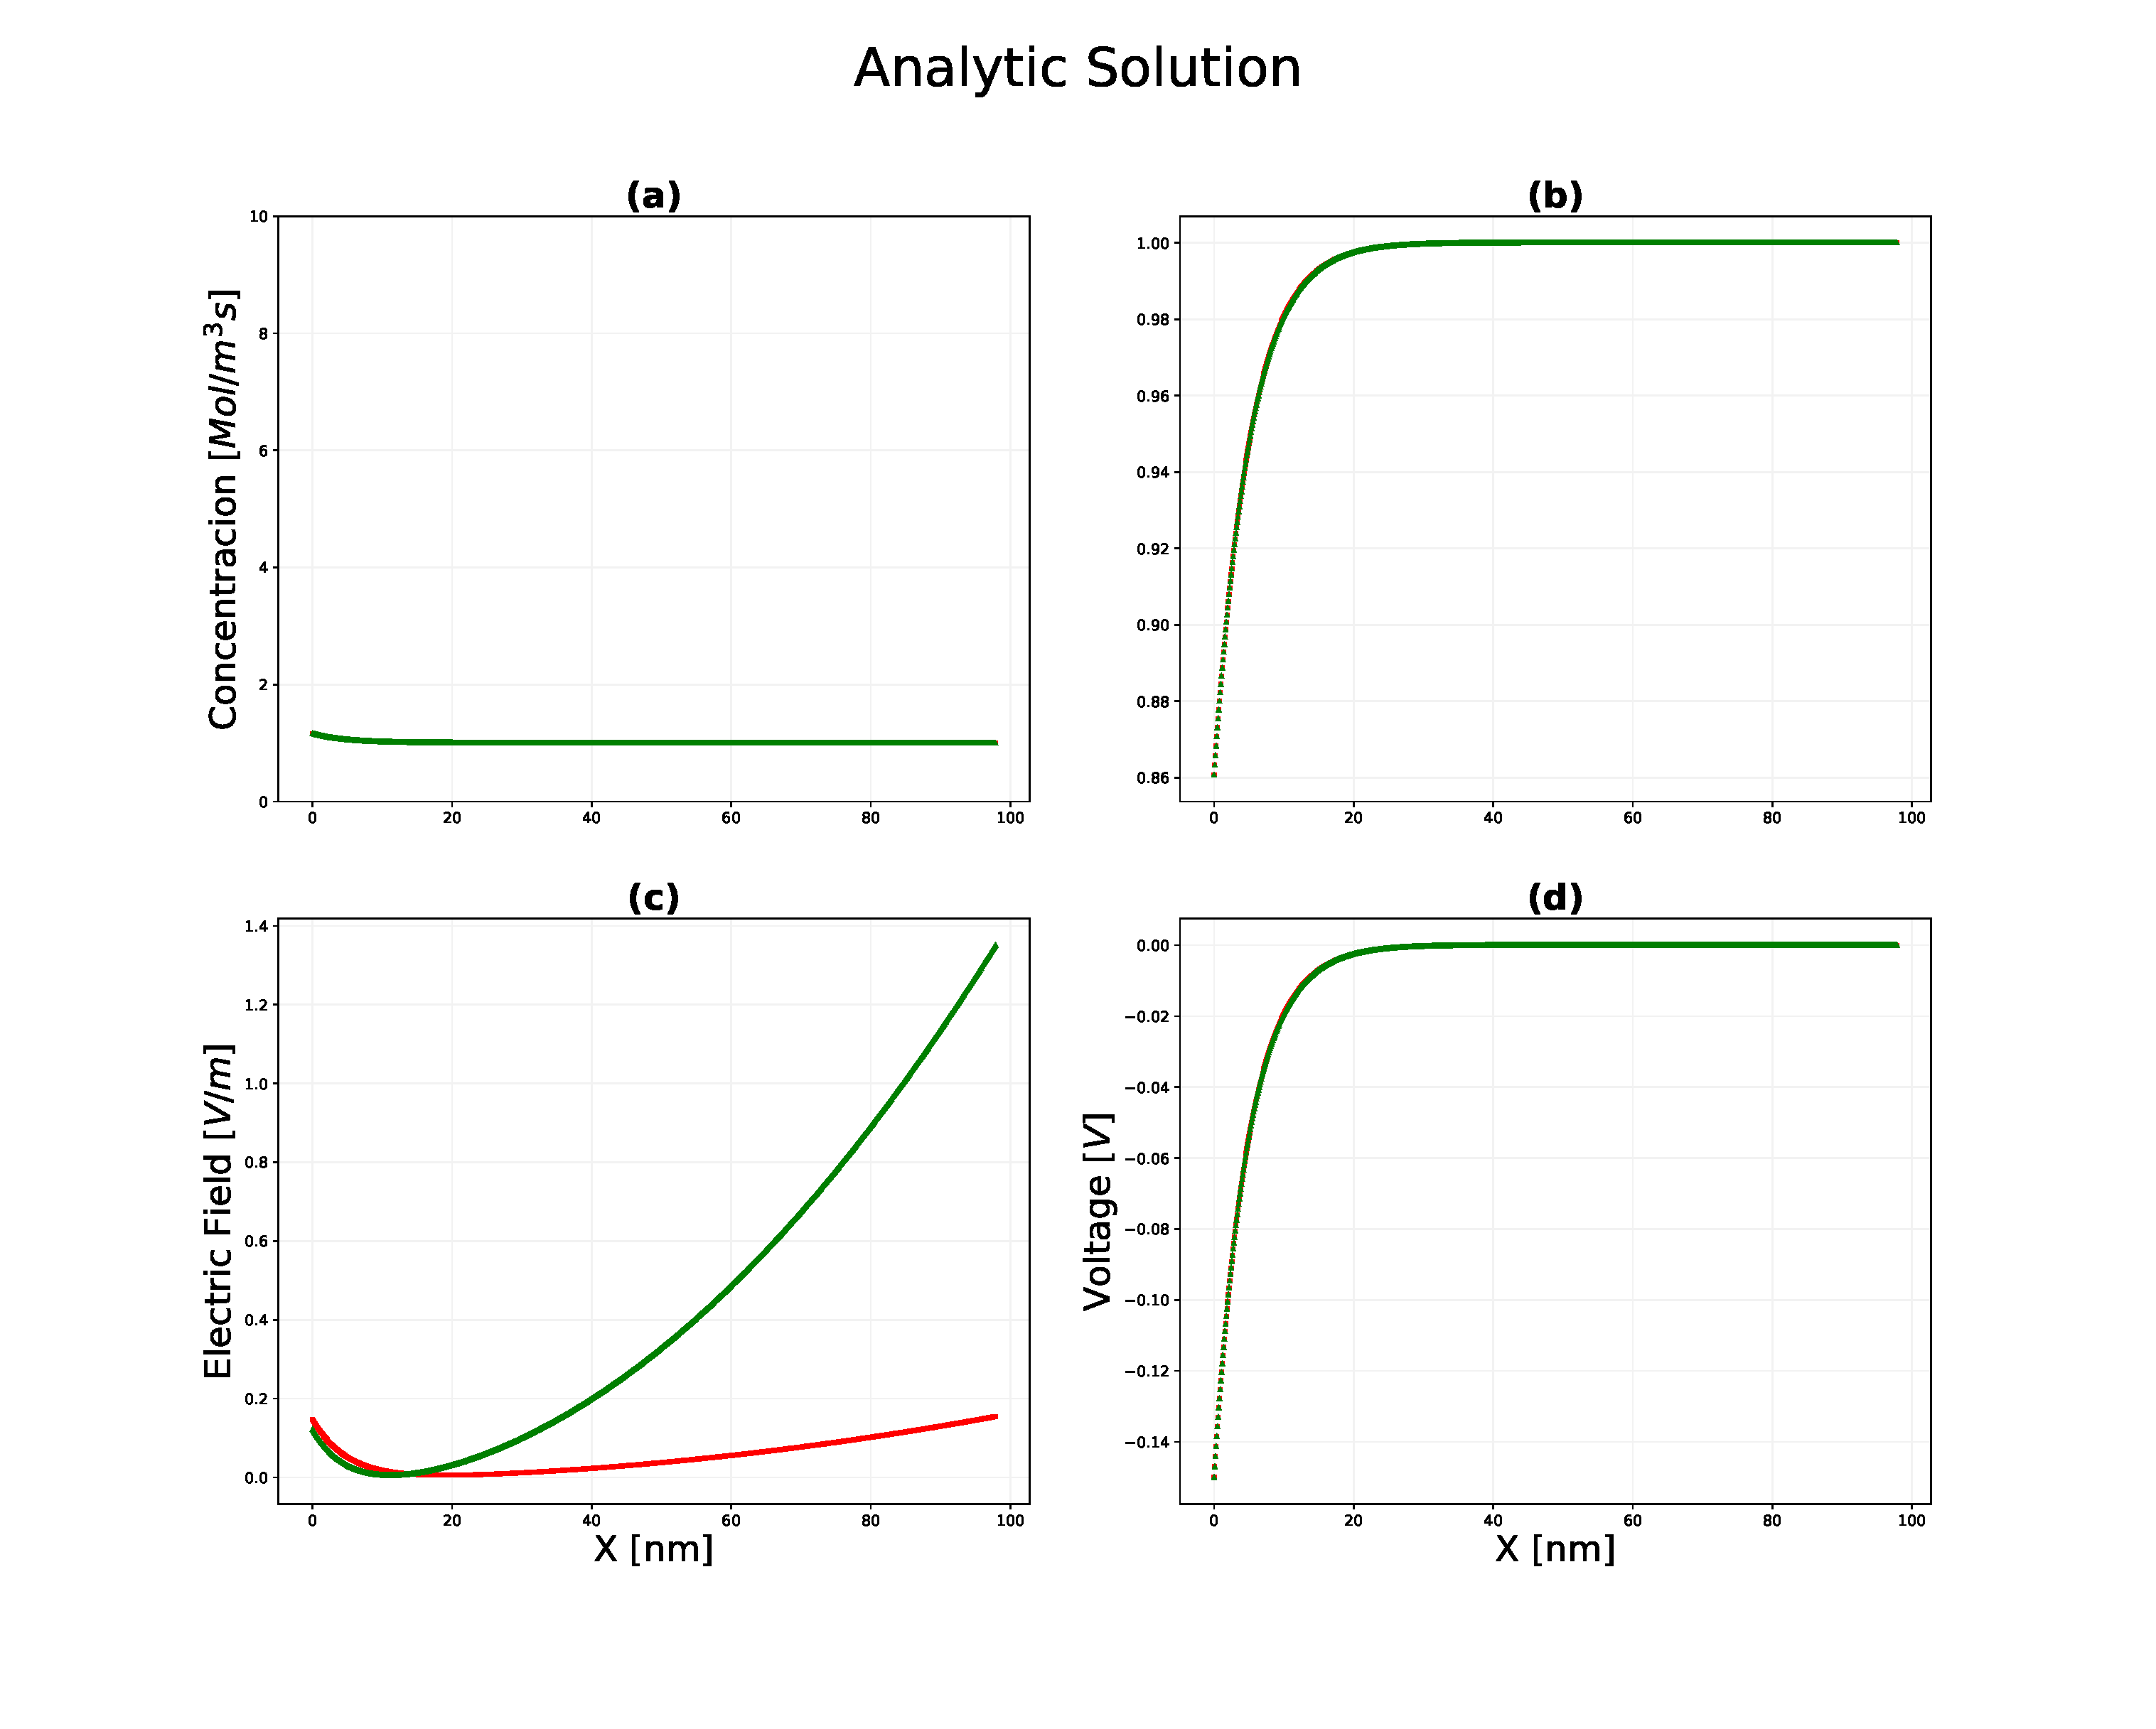
\includegraphics[width = \linewidth]{analytic-results}
 \caption{Analytic results. (a), (b) are the concentrations of each species of electrolytes. (c) is the electric potential and (d) the electric potential. Each plot is compared for 3 different values of the reactio rate.}
 \label{fig:analytic-results}
\end{figure}







\section{Numerical Analysis}

In order to validate the approximations made in previous sections, we solve system \ref{eq:system} numerically. In order to do so, we use the Runge-Kutta Method of order 4 along with the  Shooting Method to solve the two point boundary value (reference to Numerical Methods in python).  



The complexity of the problem lies exactly in the two point boundary feature of the problem, where the concentrations are known in the bulk, but the potential is known at the interface(see Fig. \ref{fig:geometry}). 

The approach used in these type of problems is transforming the second order system \ref{eq:system} into a first order one,

\begin{eqnarray}
C'_+(x)-\frac{zF}{RT}E(x)C_+(x) &=& -r, \\
C'_-(x)+\frac{zF}{RT}E(x)C_-(x) &=& 0, \\
E'(x) &=& \frac{zF}{\epsilon}(C_+(x)-C_-(x)), \\
\phi'(x) &=& -E(x).
\label{eq:linear-system}
\end{eqnarray}

subject to the border conditions

\begin{eqnarray}
C_+(\delta) &= C_b,  \\
C_-(\delta) &= C_b, \\
\phi(\delta) &=& 0\\
\phi(0) &=&  V_0
\label{eq:linear-system}
\end{eqnarray}

Here the primes denote derivatives with respect to $x$. Once the system is in the form of Eqn. \ref{eq:linear-system}, we can apply the Runge-Kutta Method with the shooting method to obtain the numerical solutions. 


\section{Results}

Fig. \ref{fig:numeric-results} show the results obtained. The solution of the steady state at different values of the reaction rate do not defer much closest to the surface of the electrode ($x=0$). Also, from Fig. \ref{fig:numeric-results} (c) and (d) we can see that the aproximation of the electric field and the electric potential is fairly 

\begin{figure}[htbp]
 \centering
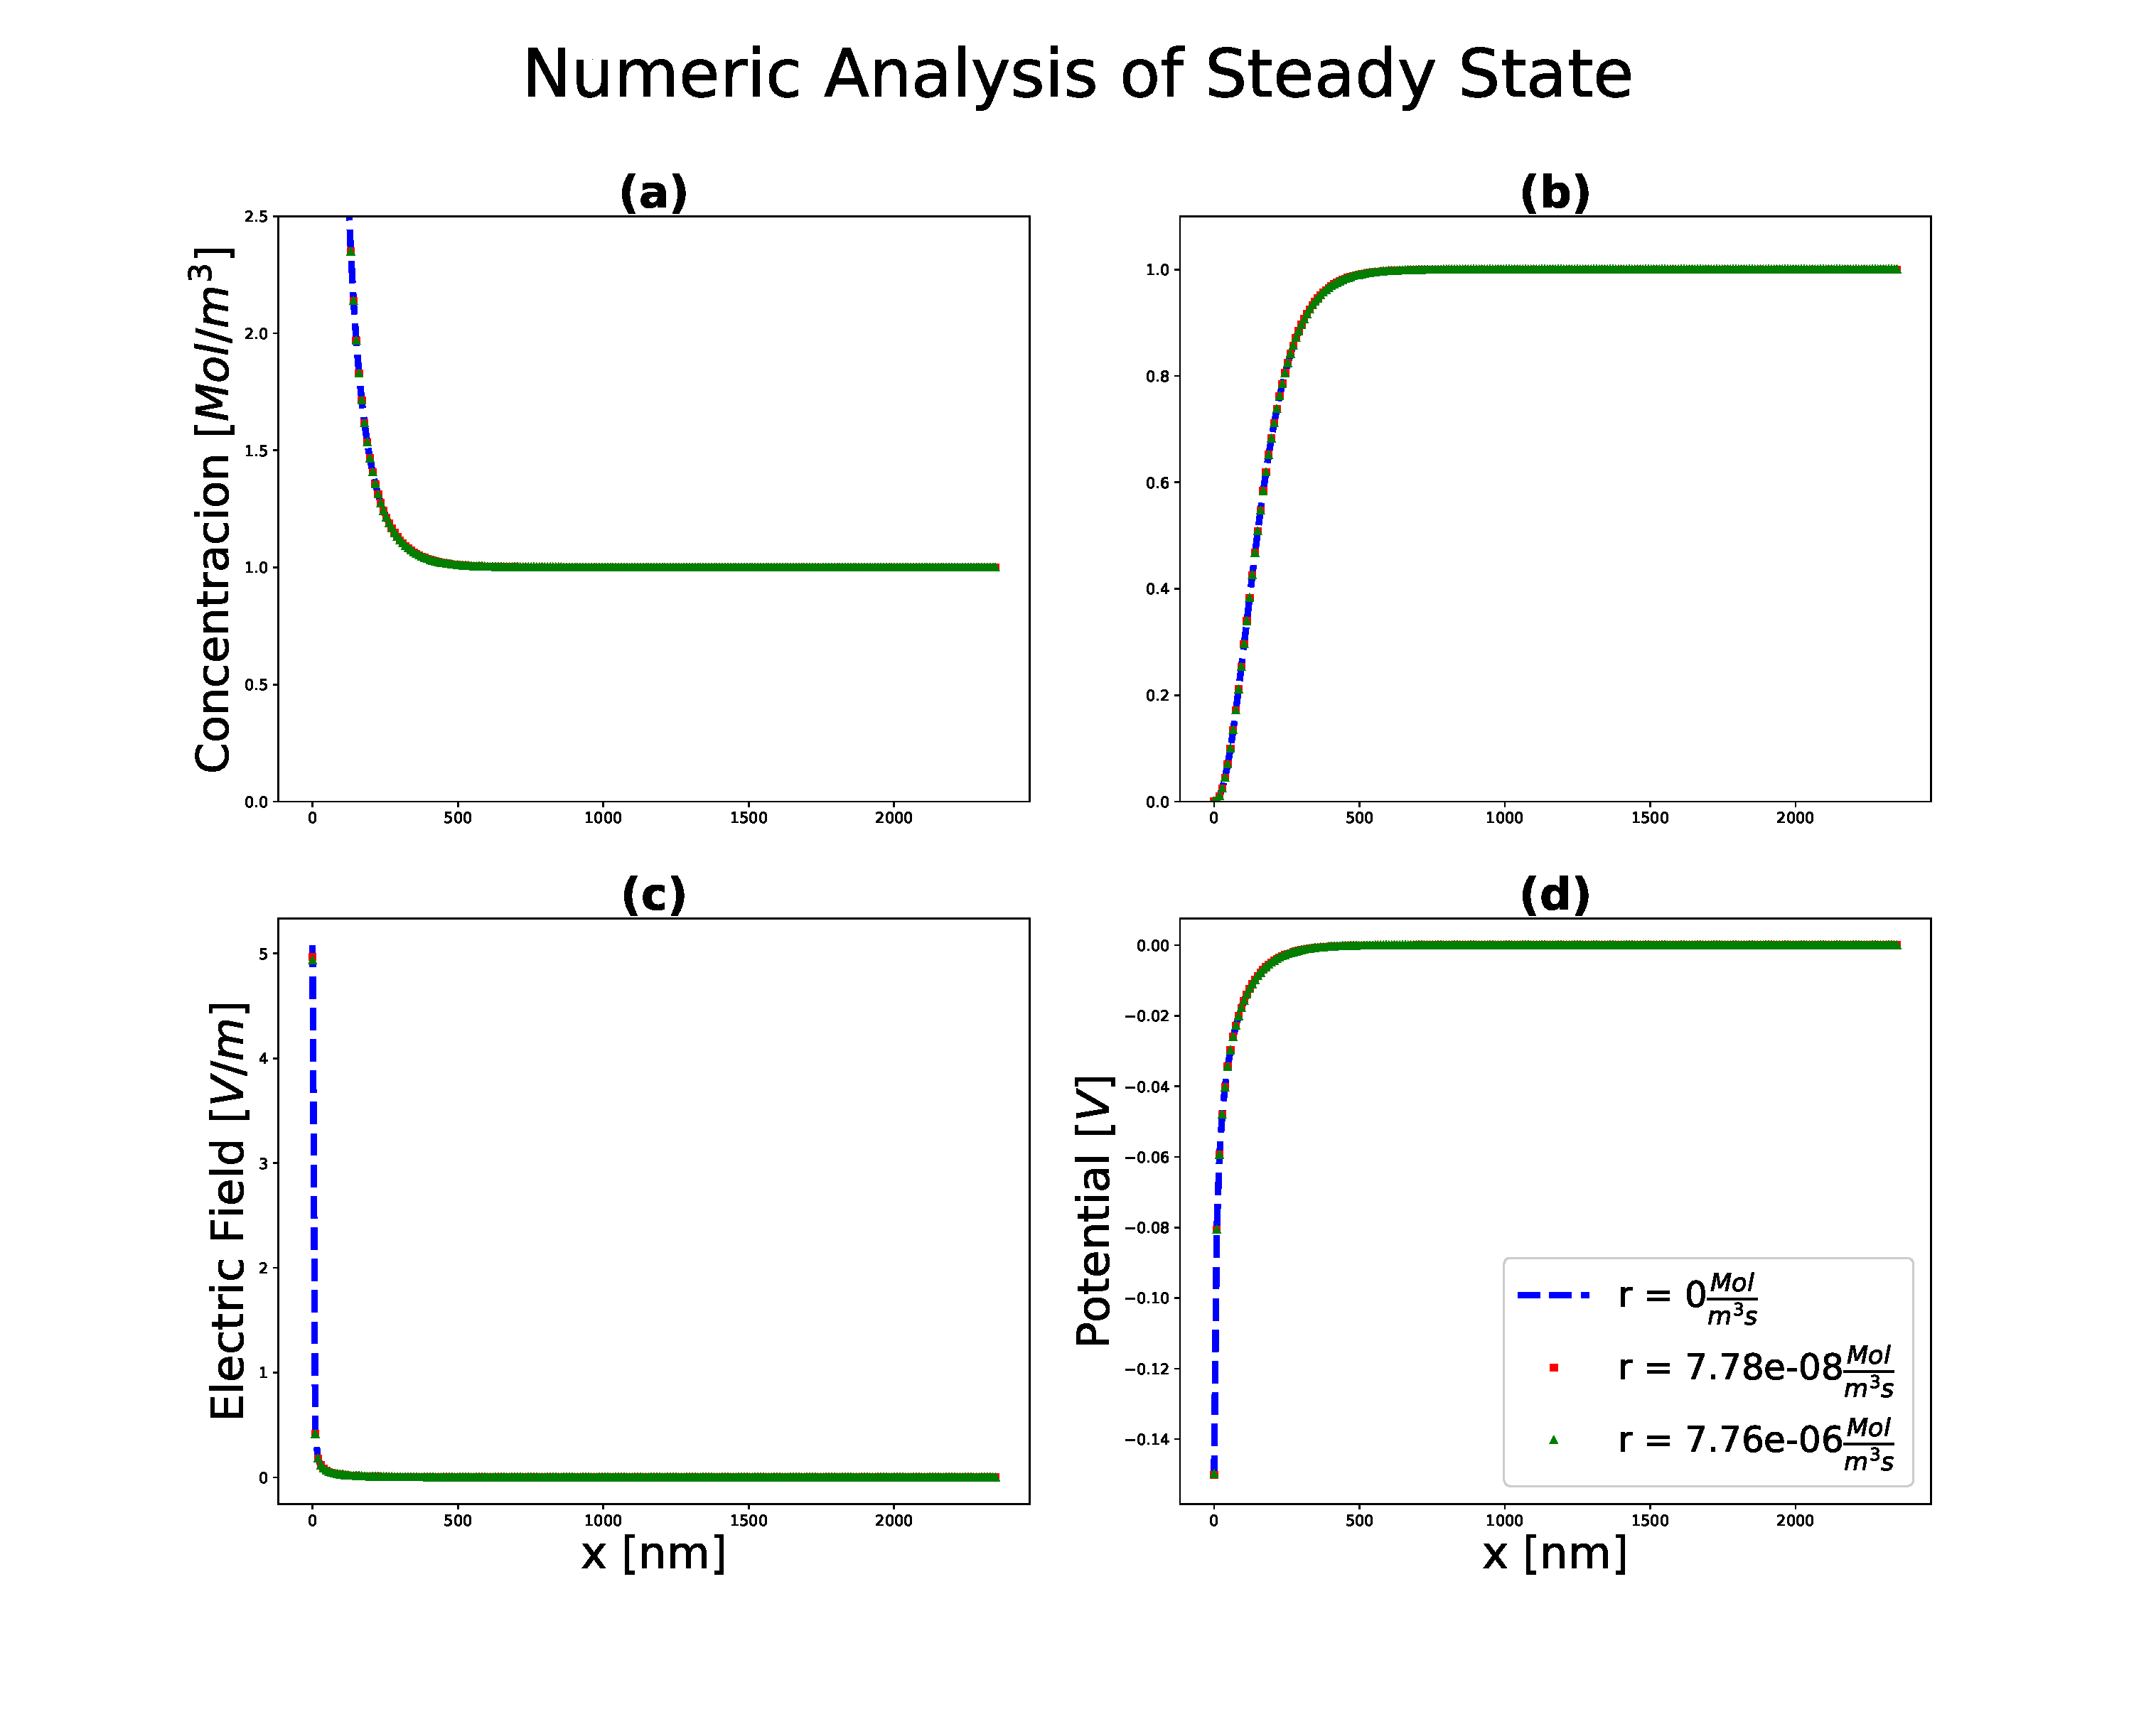
\includegraphics[width = \linewidth]{results-numeric}
 \caption{The numerical and the analytic solution to the potential to first order in the current.}
 \label{fig:numeric-results}
\end{figure}

Dealing with the equations as presented in Eq. \ref{eq:system} is extremely difficult when doing a numerical analysis. This is due to the fact that the natural units of the system (x which is measured in meters) are too small for the computer to handle. Also, non-linearity gives extreme fluctuations of the concentration of the positive ion near the surface. Since we where using the shooting method, we needed to change the values of the electric field at the bulk, such that the boundary condition for the electric potential is correct, but this induced such strong concentrations at the interface sometimes, that the computer could not handle the numbers resulting from Runge-Kutta method. We had to make a little adaptation in order to be able to find the correct boundary condition for the electric field with the shooting method. 




As it can be seen in figures  \ref{fig:numerical-phi},  \ref{fig:numerical-E}, the electric field and potential approach zero when the start moving into the bulk of the solution, as expected. The further away from the interface we go, the better the border conditions for the electric field are met. For our particular case, we cut the integration range when we reached a tolerance of $ E_{bulk} < 1\times 10^{-3}$, where $E_{bulk}$ is the border condition of the dimensionless electric field at the bulk. 



A similar analysis can be done for the concentrations (Fig.  \ref{fig:numerical_c}), but this time the value of both concentrations at the bulk is $C_b$, as defined by the border conditons for the system \ref{eq:system}.



Another difficulty is that, since we used the adaptive Runge-Kutta method, the concentrations change so abruptly that the adaptive step $h$ becomes increadibly small. The problem with this is that the number of iterations needed with a step of the order of $h\approx 10^{-29}$. In order to reach the full length of integration is too big and therefore, we obtain only a part of the integration interval and not as close to the interface as we should like. 

To avoid such difficulties, we have worked with the adimensional potential in a scale of adimensional length $\xi = \kappa x$. We have integrated on the interval $[0, 20 \kappa \delta]$.





\chapter{Dynamic Solution}
\section{Analytic Solution}

Consider know the dynamical model in which time dependence is not neglected

\begin{eqnarray}
	\frac{\partial C_+}{\partial t} = D_+\qty{\frac{\partial^2 C_p}{\partial x^2} - \frac{\partial}{\partial x}\qty{C_+\frac{\partial\Psi}{\partial x}}} \\
	\frac{\partial C_+}{\partial t} = D_+\qty{\frac{\partial^2 C_p}{\partial x^2} - \frac{\partial}{\partial x}\qty{C_+\frac{\partial\Psi}{\partial x}}} \\
	\nabla^2 \Psi = -(C_+-C_-)
\end{eqnarray}

By making the following change of variables 

\begin{eqnarray}
	\xi = \frac{\kappa x}{\sqrt{4Dt}}\\
	\frac{\partial \xi}{\partial x} = \frac{\kappa}{\sqrt{4Dt}}\\
	\frac{\partial \xi}{\partial x} = -\frac{\kappa x}{2\sqrt{4Dt^3}}
\end{eqnarray}

we can re-write the system of equations as

\begin{eqnarray}
	\label{eq:sys_dyn1}
	\frac{\partial^2 C_+}{\partial \xi^2} + \frac{2\xi}{\kappa}\frac{\partial C_p}{\partial \xi}  -\frac{\partial C_+}{\partial \xi}\frac{\partial \Psi}{\partial x}-C_+\frac{\partial^2\Psi}{\partial \xi^2} \\
	\label{eq:sys_dyn2}
	\frac{\partial^2 C_+}{\partial \xi^2} + \frac{2\xi}{\kappa}\frac{\partial C_p}{\partial \xi}  +\frac{\partial C_+}{\partial \xi}\frac{\partial \Psi}{\partial \xi}+C_+\frac{\partial^2\Psi}{\partial \xi^2} \\
	\label{eq:sys_dyn3}
	\nabla^2 \Psi + 4Dt(C_+-C_-) = 0
\end{eqnarray}

In order to solve the previous system, we will integrate equations \ref{eq:sys_dyn1} and \ref{eq:sys_dyn1}. Lets write the two equations as one in terms of the charge of the electrolyte $s=\pm$.

\begin{equation}
	\frac{\partial^2 C_s}{\partial \xi^2} + \frac{2\xi}{\kappa}\frac{\partial C_s}{\partial \xi}  -s\frac{\partial C_s}{\partial \xi}\frac{\partial \Psi}{\partial \xi}-sC_s\frac{\partial^2\Psi}{\partial \xi^2}
\end{equation}

Since,

\begin{equation}
	\int_0^\xi \frac{\partial C_s}{\partial \xi} = \xi C_s(\xi) - \int_0^\xi C_s(\xi) d\xi
\end{equation}
\begin{equation}
	\int_0^\xi \frac{\partial C_s}{\partial \xi}\frac{\partial \Psi}{\partial \xi} = \frac{\partial \Psi}{\partial \xi} C_s - \int_0^\xi C_s(\xi) \frac{\partial^2 \Psi}{\partial \xi^2} d\xi
\end{equation}

We get,

\begin{equation}
	\frac{\partial C_s}{\partial \xi} + \frac{2\xi}{\kappa} - \frac{2}{\kappa} \int_0^\xi C_s(\xi)-s\frac{\partial C_s}{\partial \xi}\frac{\partial \Psi}{\partial \xi} = 0
\end{equation}

Dividing the equation by $C_s$, which should be always possible, we get

\begin{equation}
\frac{1}{C_s}\frac{d C_s}{d\xi} = \frac{-2}{\kappa}\xi + \frac{2C_s}{\kappa}\int_0^\xi C_s(\xi) d\xi + s\frac{\partial \Psi}{\partial \xi}	
\end{equation}

Integrating we get

\begin{equation}
	\log\qty{\frac{C_s}{C_s(0)}} = -\frac{\xi^2}{\kappa} + \Psi + \frac{2}{\kappa} \int_0^\xi C_s(z)\int_0^z C_s (z')dz' dz
\end{equation}

From the Poisson Equation \ref{eq:sys_dyn3} we get

\begin{eqnarray*}
	C_s(\xi) = C_{-s}-\frac{s}{4Dt}\frac{\partial^2 \Psi}{\partial \xi^2}
\end{eqnarray*}

We make the approximation that $C_+ << C_-$ near the interface. Therefore

\begin{equation}
	\int_0^\xi C_s(z)\int_0^z C_s (z')dz' dz \approx \int_0^\xi  dz \frac{1}{(4Dt)^2}\Psi' \Psi '' = \frac{1}{(4Dt)^2}\qty{\frac{\partial \Psi}{\partial \xi}}^2
\end{equation}

Therefore, the concentration for each species in terms of the potential an the electric field is

\begin{equation}
	C_s = C_b e^{-\frac{1}{k}\qty{\xi^2 - \frac{E^2}{8D^2t^2}}}  e^{s\Psi}
\end{equation}

\section{Potential}

Now we solve for the electric potential. The Poisson equation in terms of the previously found concentration profiles is

\begin{equation}
	\frac{\partial^2 \Psi}{\partial \xi^2} = -2C_be^{\frac{1}{2}{\xi^2-\frac{E^2}{8D^2t^2}}}\sinh{\Psi}
\end{equation}

This can be written as

\begin{equation}
	e^{-\frac{E^2}{8D^2t^2\kappa}}\Psi'' = -2C_b e^{\frac{\xi^2}{\kappa}}\sinh{\Psi}
\end{equation}

Integrating over $\xi$ we get

\begin{equation}
	\frac{\sqrt{\pi}}{2}\erf(\sqrt{\alpha}\Psi')\qty{-\frac{4Cb}{\sqrt{\pi}}\int_0^\xi e^{-\frac{s^2}{\kappa}}\sinh{\Psi(s)}ds}
\end{equation}


\begin{equation}
	\Psi'= \frac{1}{\sqrt{\alpha}}\erf^{-1}\qty{-\frac{4Cb}{\sqrt{\pi}}\int_0^\xi e^{-\frac{s^2}{\kappa}}\sinh{\Psi(s)}ds}
\end{equation}

Integrating and using the properties of the $\erf^{-1}$ function we get

\begin{equation}
	\Psi'= \frac{1}{\sqrt{\pi\alpha}}\erf^{-1}\qty{-\frac{4Cb}{\sqrt{\pi}}\int_0^\xi e^{-\frac{s^2}{\kappa}}\sinh{\Psi(s)}ds}
\end{equation}













\subsection{Numeric Solution To The Diffusion Only Equation}


\par As a first approach to the problem, we will use an implicit scheme to find the numerical solution. This means that, in approaching the finite difference method, we will compute the spacial derivative at time step $n+1$. 
Just as in the analytic case, we define
\begin{align}
	\rho(x,t) = \frac{C(x,t) - C_b}{C_b},
\end{align}

which will make the numerical computations converge faster.



Consider the one dimensional diffusion equation

\begin{align}
\frac{\partial \rho}{\partial t} &= D \frac{\partial^2 \rho}{\partial x^2}.
\label{eq:diffusion}
\end{align}

We will define $x = \delta \xi$ where $\delta$ is the width of the laminar flow sheet. 

\begin{align}
\frac{\partial \rho}{\partial t} = \frac{D}{\delta^2} \frac{\partial^2 \rho}{\partial \xi^2},\\
\frac{\partial \rho}{\partial \tau} = \frac{\partial^2 \rho}{\partial \xi^2},
\end{align}

where we have defined $\tau = Dt/\delta^2$, which follows the modified border and initial conditions,

\begin{align}
	\rho(\xi = 1, \tau) = 0, \\
	D \frac{\partial \rho}{\partial \xi} (\xi = 0, \tau) = 0,\\
	\rho(\xi, \tau = 0) = -1.
\end{align}


We will discretize the derivative as follows,

\begin{align}
\frac{\partial \rho}{\partial \tau}^{n+1, k}= \frac{C^{n+1, k}-\rho^{n, k}}{\Delta \tau},\\
\frac{\partial^2 \rho}{\partial \xi^2}^{n+1, k} = \frac{\rho^{n+1, k-1}-2\rho^{n, k}+\rho^{n+1, k+1}}{\Delta \xi^2}.
\end{align}

Replacing these approximations into equation \ref{eq:diffusion} we get

\begin{align}
    -\alpha \rho^{n+1,k-1} + ( 1 + 2\alpha ) \rho^{n+1,k} -\alpha \rho^{n+1,k+1} =  \rho^{n,k}\\
    k \in [1, ... , m-1]
    \label{eq:equations-n}
\end{align}

In particular, for a given $n$ value,  the equations for $k=1$ and $k=m-1$ (which include the border conditions) are

\begin{align}
    -\alpha \rho^{n+1,0} + ( 1 + 2\alpha ) \rho^{n+1,1} -\alpha \rho^{n+1,2} = \rho^{n,1},\\
    -\alpha \rho^{n+1,m-2} + ( 1 + 2\alpha ) \rho^{n+1,m-1} -\alpha \rho^{n+1,m} = \rho^{n,m-1}.
    \label{eq:border-equations}
\end{align}

The border conditions for our system (in discretized form) are

\begin{align}
    \rho^{n, 0} = \rho^{n, 1}, \\
    \rho^{n, m-1} = 0.
\end{align}

Therefore, equations \ref{eq:border-equations} yield

\begin{align}
    ( 1 + \alpha ) \rho^{n+1,1} -\alpha \rho^{n+1,2} = \rho^{n,1},\\
    -\alpha \rho^{n+1,m-2} + ( 1 + 2\alpha ) \rho^{n+1,m-1} = \rho^{n,m-1}.
\end{align}

We want to put these equations in matrix form. Let 

\begin{align}
    \bf{\rho^n} = \begin{bmatrix}
                    \rho^{n, 0} \\
                    \rho^{n, 1} \\
                    \vdots \\
                    \rho^{n, m-1} \\
                    \rho^{n, m} \\
                    \end{bmatrix},
\end{align}

and 

\begin{align}
\bf{\underline{A}} &= \begin{bmatrix}
           ( 1 + \alpha ) & -\alpha  &  0 & 0 &  \cdots & 0\\
             -\alpha & ( 1 + 2 \alpha ) & -\alpha & \cdots & 0 & 0\\
           \vdots  &\cdots  & \ddots & \ddots &  \ddots&  \\
            \vdots & \cdots & 0  &  -\alpha & ( 1 + 2 \alpha ) & -\alpha \\
            0 & \cdots &0  & 0 & -\alpha & ( 1 + 2 \alpha )
         \end{bmatrix}
         \label{eq:discretization-matrix}.
\end{align}

Equations \ref{eq:equations-n} can be expressed as

\begin{align}
    \bf{\underline{A}} \bf{\rho^{n+1}}  = \bf{\rho^n} .
\end{align}

Considering the initial conditions \ref{eq:initial-condition}, we get

\begin{align}
    \bf{\rho^{0,k}} = -C_b, \\
    k \in [1,..., M-1].
\end{align}

This means that the shape of $\bf{\underline{A}}$ is $M-2 \times M-2$ and the numerical solution is solved in the interval  $k \in [0,..., M]$, leaving $k=0$ and $k=M$ as the overflow terms to push the boundary conditions. Nevertheless, these terms must be included in order to get the full solution (otherwise we should start from $k=1$ and end at $k=M-1$ and not include the border conditions in the plot of our numeric result).

Now we are ready to start iterating this matrix equation to get the time evolution.

We will use the parameters $\xi = x/\delta$ and $\tau = t/\delta^2$ as the parameters of the equation. The comparison between numeric and analytic results is shown in figure ]ref{diffusion-comparison}.

\begin{figure}[htbp]
\centering
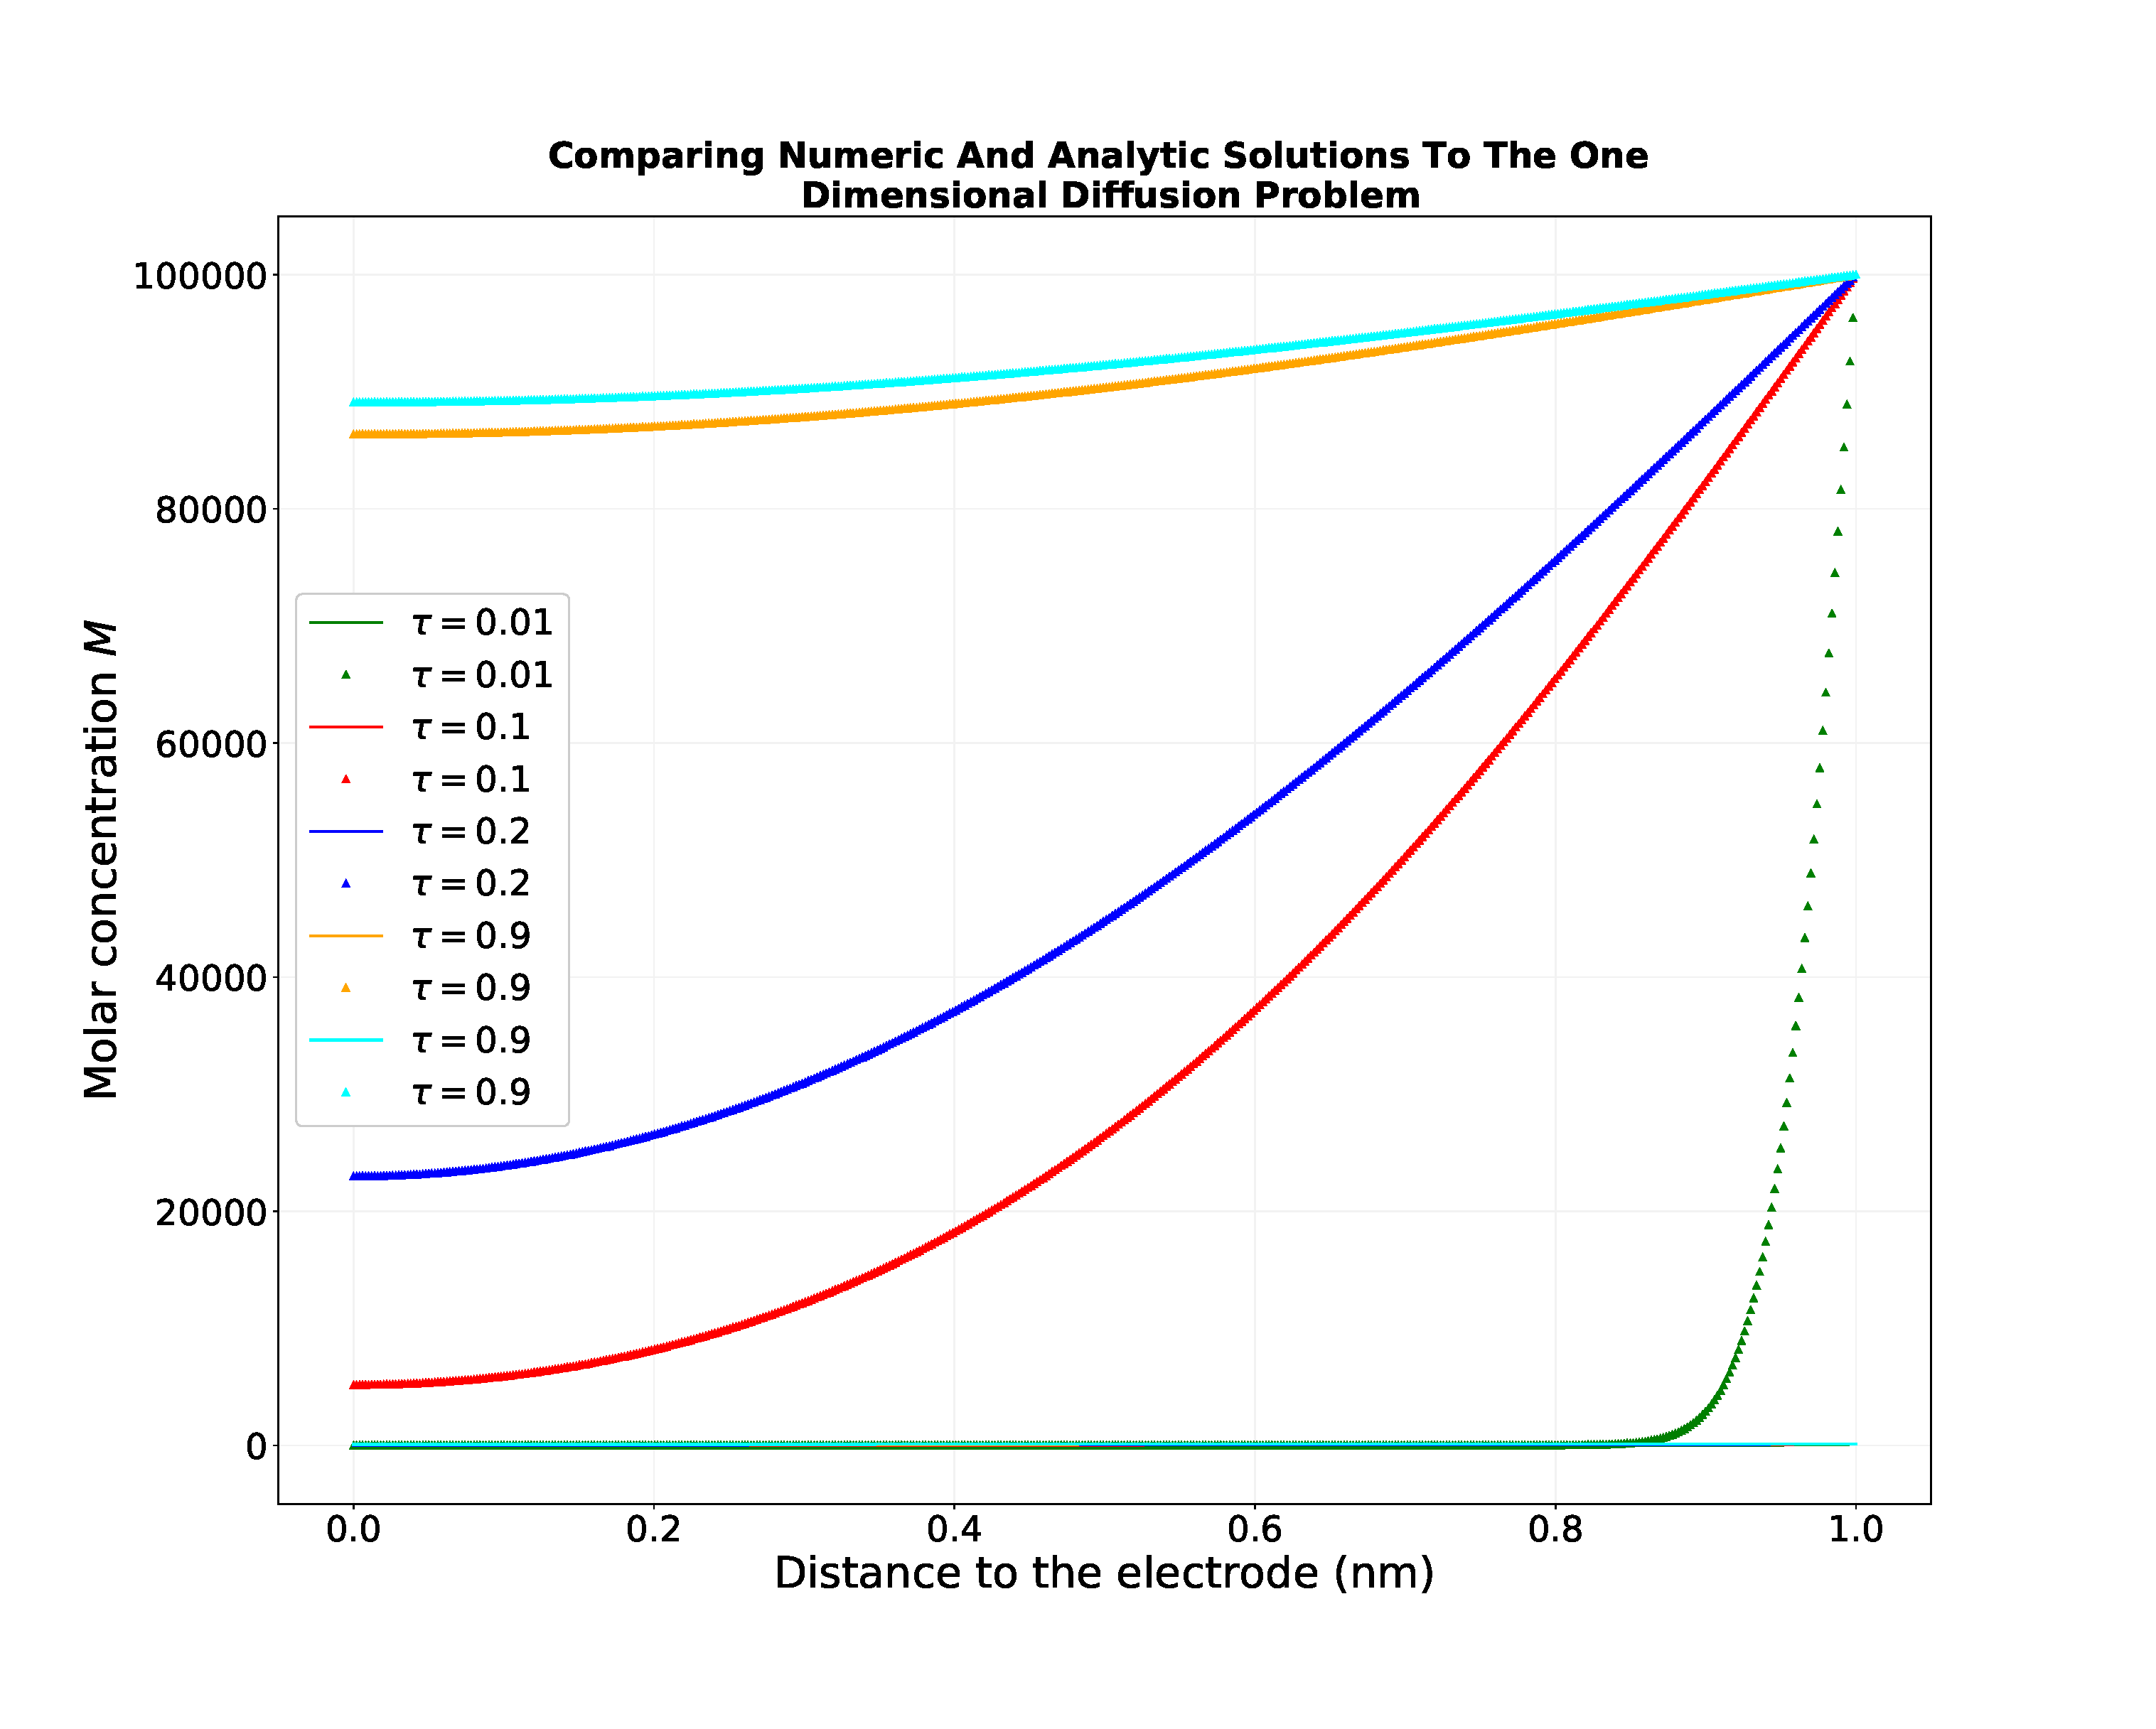
\includegraphics[width=\textwidth]{concentration-diffusiononly-comparison}
\caption{}
\label{fig:diffusion-comparison}
\end{figure}



\section{Diffusion Reaction Equation}
\label{sec:analytic-diffusion-reaction}
In this section we compute the analytic solution to the diffusion equation, subject to a chemical reaction at the interface ($x = 0$).
We need to solve the equation

\begin{align}
\label{eq:diffusion-only}
	\frac{\partial C}{\partial t} = D\frac{\partial^2 C}{\partial x^2},
\end{align}

which must meet the border conditions

\begin{align}
\label{eq:border-conditions-reaction-diffusion}
	C(x = \delta, t) = C_b,\\
	-D\frac{\partial C(x = 0, t)}{\partial x} = -r,
\end{align}

and the initial condition

\begin{align}
	C(x, t = 0) = 0.
\end{align}


In Appendix \ref{appendix:diffusion-reaction-only} we have outlined the algorithm and the analytic solution to this problem. The analytic solution is

\begin{align}\nonumber
	C(t, x) = C_b\qty{1- \frac{4}{\pi} \sum_{n=0}^\infty \frac{(-1)^n}{(2n+1)}\exp\qtys{-\qty{\frac{(2n+1)\pi}{2}}^2\frac{D_- t}{\delta^2}}\cos\qty{\frac{(2n+1)\pi}{2} \frac{x}{\delta}}}\\ -\frac{r\delta}{D}\qty{1-\xi - \frac{8}{\pi^2}\sum_{n=0}^\infty \frac{1}{(2n+1)^2}\exp\qtys{-\qty{\frac{(2n+1)\pi}{2}}^2\frac{D_- t}{\delta^2}}\cos\qty{\frac{(2n+1)\pi}{2} \frac{x}{\delta}}}.
	\label{eq:solution-diffusion-reaction}
\end{align}

Numeric and analytic results are plotted in Fig. \ref{fig:diffusion-reaction-comparison-fixed-r}
\newpage
\begin{figure}[htbp]
\centering
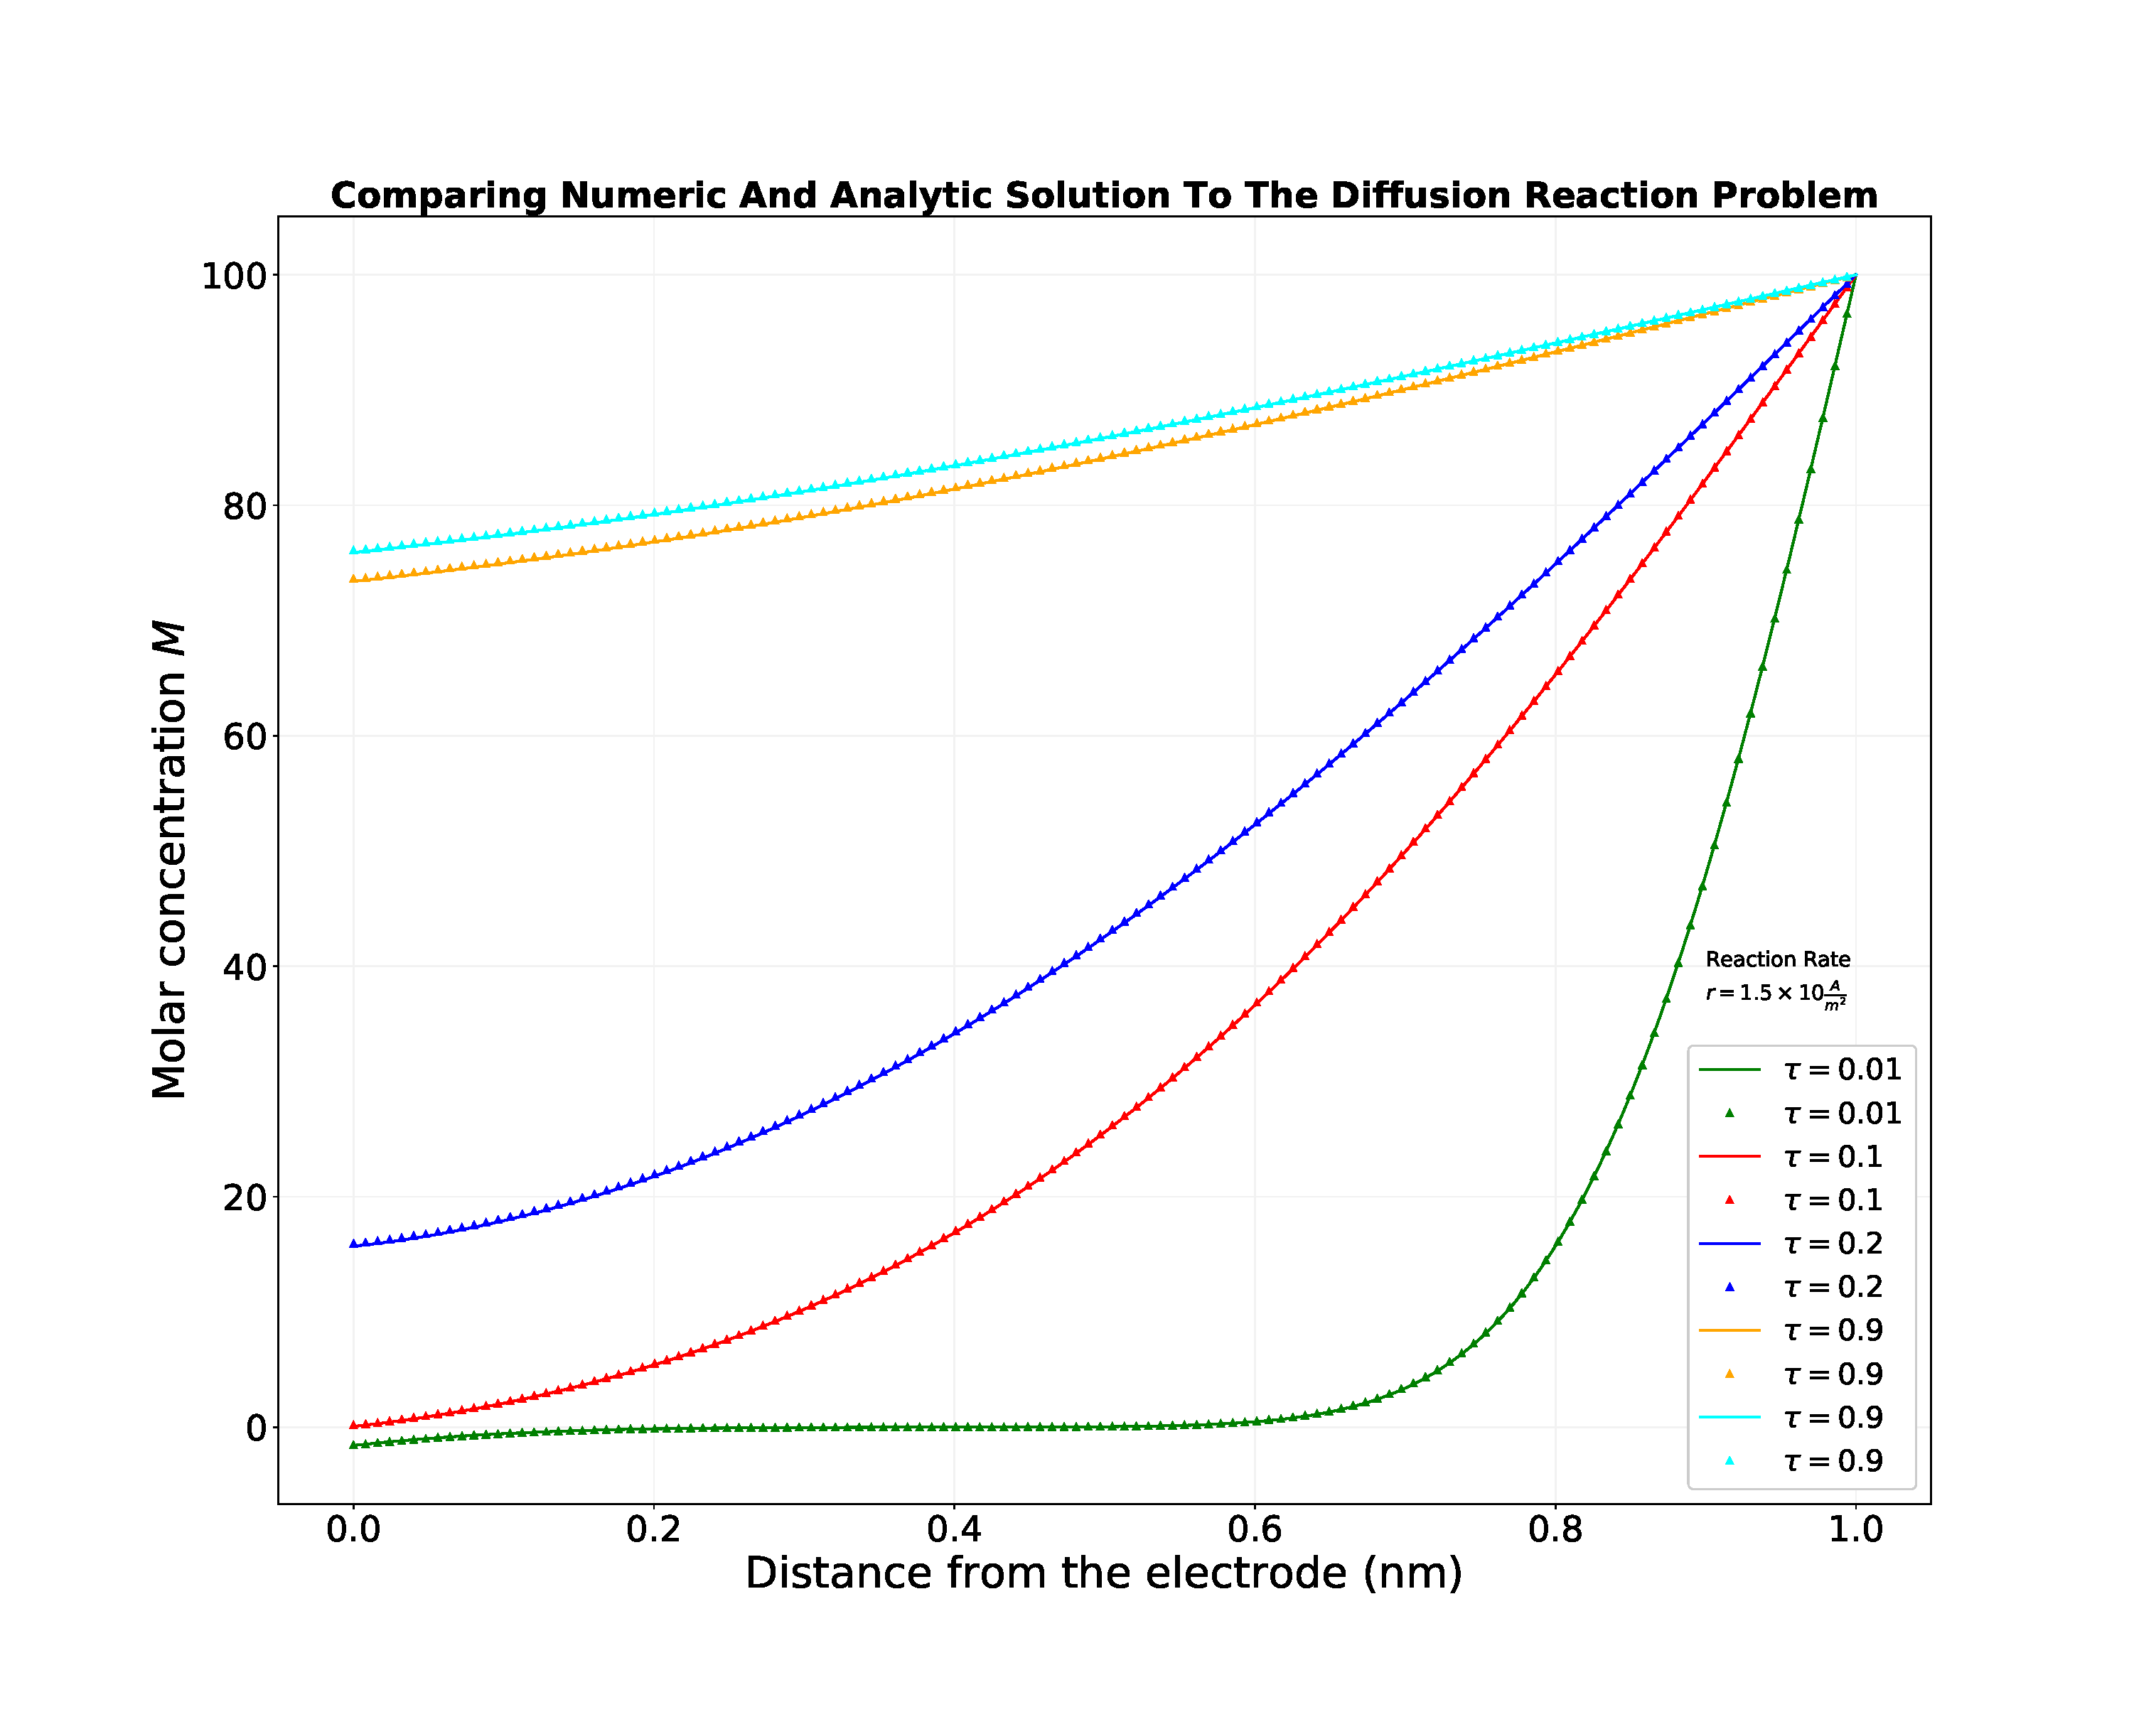
\includegraphics[width=\textwidth]{diffusion-reaction-comparison}
\caption{Each curve represents the concentration profile at increasingly large $t$. Continuos lines represent the analytic solution at each time step and the discrete markers listed in the image legend are represent the numerical solution. Steady State in the diffusion-only problem will be when concentration is $C_b=1$ throughout the domain.}
\label{fig:diffusion-reaction-comparison-fixed-r}
\end{figure}



\newpage
\section{Diffusion-Reaction Equation With Forced Current through the system.}

We consider the same system as above

\begin{align}
	\frac{\partial C}{\partial t} = \frac{\partial^2 C}{\partial x^2},
\end{align}

with a slight change in border conditions. We want to impose the current on the system, which should be proportional to the reaction rate at the interface.

\begin{align}
	R &= k_f C(0^+, t)\\ 
	&= \frac{i_0}{\mathcal{F}}.
\end{align}

This yields the following border and initial conditions for the problem

\begin{align}
	C(\delta, t) &= C_b,\\
	C(0^+, t) &= \frac{R}{k_f},\\
	C(x, 0) &= 0.
\end{align}

or equivalently

\begin{align}
	C(\delta, t) &= C_b,\\
	C(0^+, t) &= \frac{i_0}{\mathcal{F}k_f},\\
	C(x, 0) &= 0.
\end{align}

\subsection{Steady State Solution}

As always, first we compute the steady state solution.

\begin{align}
	\frac{d ^2C}{d x^2} = 0.
\end{align}

The solution is of the form

\begin{align}
	C_{SS}(x) = A + Bx.
\end{align}

Border conditions yield,

\begin{align}
	C_{SS}(\delta) &= A + B\delta\\
	&= C_b,
\end{align}

and

\begin{align}
	C_{SS}(0) &= A \\
	&= \frac{i_0}{\mathcal{F} k_f}.
\end{align}

Therefore,

\begin{align}
	C_{SS} (x) = \frac{i_0}{\mathcal{F}k_f} +\qty{C_b - \frac{i_0}{\mathcal{F}k_f}}\frac{x}{\delta}
\end{align}

\subsection{Dynamic Solution}

To solve the dynamic solution, we consider the following change of variable

\begin{align}
	\rho(x, t) = \frac{C(x,t)-C_{SS}(x)}{C_b}.
\end{align}

As in previous sections, we define the dimensionless parameters $\tau = \frac{\mathcal{D} t}{\delta^2}$, $\xi = \frac{x}{\delta}$. This leads to the equation

\begin{align}
	\frac{\partial \rho}{\partial \tau} = \frac{\partial^2 \rho}{\partial \xi^2}.
\end{align}

Let $\rho(\xi, \tau)$ be of the form

\begin{align}
	\rho(\xi, \tau) = F(\xi)G(\tau).
\end{align}


Separation of variables leads to the Sturm-Liouville problem

\begin{align}
	\frac{d G}{d \tau} + \lambda^2G(\tau) = 0,
	\label{eq:G-eq}\\
	\frac{d^2 F}{d\xi^2} + \lambda^2 F(\xi) = 0.
	\label{eq:F-eq}
\end{align}


The solution of \ref{eq:G-eq} is 

\begin{align}
	G(\tau) = G(0) e^{-\lambda^2 \tau},
\end{align}

whereas for \ref{eq:F-eq} we get the particular solution,

\begin{align}
	F(\xi) = A_\lambda\sin(\lambda \xi) + B_\lambda\cos(\lambda \xi)
\end{align}

Border conditions yield 

\begin{align}
	B = 0,\\
	\lambda = n\pi.
\end{align}

where $n$ is an integer number. We let $A_n = G(0) A_\lambda$ and the general solution for $\rho$ is

\begin{align}
	\rho(\xi, \tau) = \sum_n A_n e^{-n^2\pi^2 \tau}\sin(n\pi \xi).
\end{align}


Consider the following integral

\begin{align}
	J_{n,m} = \int_0^1 \sin(n\pi\xi) \sin(m\pi\xi) d\xi.
\end{align}

It can be shown that 

\begin{align}
	J_{n,m} = \frac{1}{2}\delta_{n,m}.
	\label{eq:jnm}
\end{align}

Using \ref{eq:jnm}, we can compute the value of $A_n$ using the initial condition,

\begin{align}
	\rho(\xi, 0) &= \sum_n A_n \sin(n\pi\xi)\\
	 &= -\frac{C_{SS}(\xi)}{C_b}.
\end{align}

or equivalently,

\begin{align}
	A_n = -\frac{2}{C_b} \int_0^1 C_{SS}(\xi)\sin(n\pi\xi) d\xi.
\end{align}

Computing the integral and using \ref{eq:steady-state} we get

\begin{align}
	A_n = -\frac{2}{n\pi C_b} \qty{\frac{i_0}{k_f\mathcal{F}} - (-1)^n C_b}.
\end{align}


From which $\rho$ can be written as,

\begin{align}
	\rho(\xi, \tau) = \sum_n \frac{2}{n\pi C_b} \qty{(-1)^n C_b- \frac{i_0}{k_f\mathcal{F}}} e^{-n^2\pi^2\tau}\sin(n\pi\xi).
\end{align}


Therefore,

\begin{align}
	C(\xi, \tau) = \frac{i_0}{\mathcal{F}k_f} +\qty{C_b - \frac{i_0}{\mathcal{F}k_f}}\xi +\frac{2}{\pi}\sum_n \qty{(-1)^n C_b- \frac{i_0}{k_f\mathcal{F}}} \frac{e^{-n^2\pi^2\tau}}{n}\sin(n\pi\xi).
\end{align}


\begin{figure}[htbp]
\centering
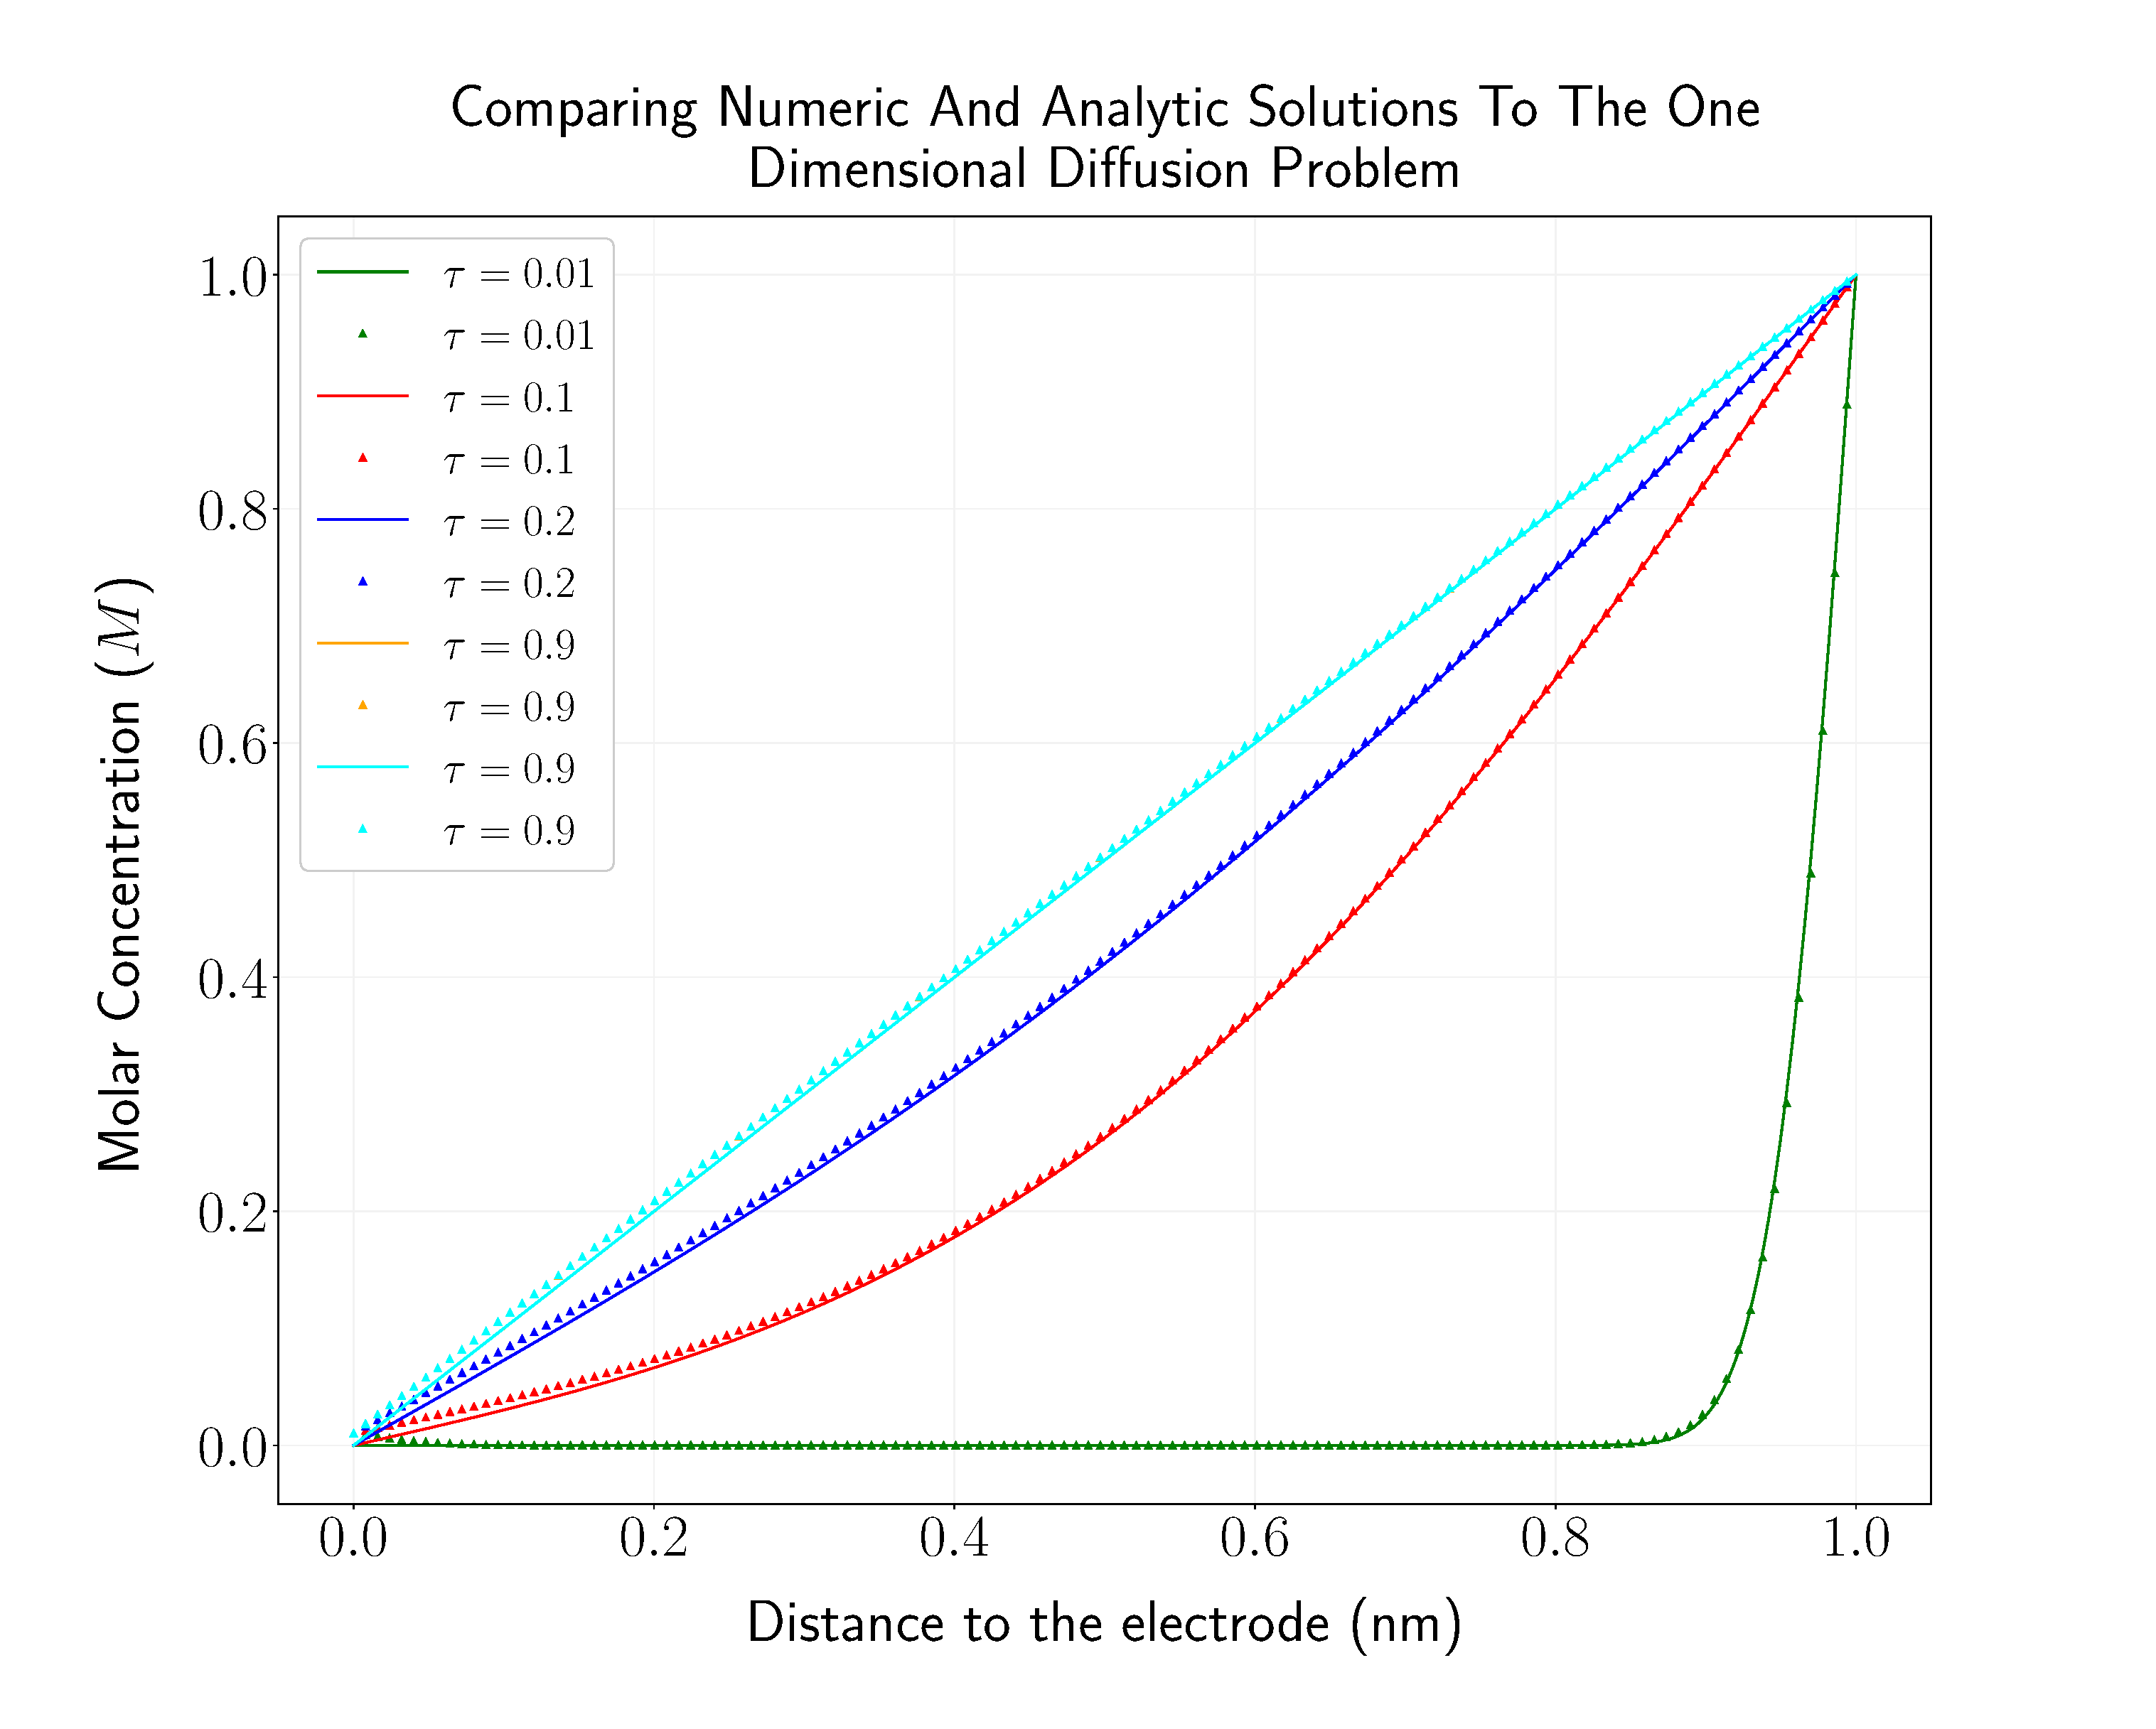
\includegraphics[width=\textwidth]{forced-current-dynamic.eps}
\caption{Comparison between numerical an analytical results. The numerical method  (dotted line) behaves as expected, following the analytical solution.}
\label{fig:diffusion-reaction-comparison}
\end{figure}

\newpage

\subsection{Numeric Solution To The Diffusion Equation With Reaction At The Interface}


For this case (s=+), we have the same equation, but border conditions at the interface change a little. We have

\begin{align}
	\rho_+(\xi = 1, \tau) = 0, \\
	D \frac{\partial \rho_+}{\partial \xi} (\xi = 0, \tau) = \frac{\delta r}{C_b},\\
	\rho_+(\xi, \tau = 0) = -1.
\end{align}

Here, we have used the adimensional parameters 

\begin{align}
    \tau = \frac{D t }{\delta ^2},\\
    \xi = \delta x
\end{align}


The approach in discretizing is exactly the same as in the previous case, with the exception of the first equation (k = 1) in which we get the following border condition

\begin{align}
    \frac{D}{\delta}\frac{\partial \rho_+}{\partial \xi} = \frac{r}{C_b}.
\end{align}

In discretized form

\begin{align}
    \frac{D}{\delta}\frac{(\rho_+^{n,1}-\rho_+^{n,0})}{\Delta \xi} = \frac{r}{C_b},
\end{align}

where $r$ is the reaction rate. In discretized form, this border condition can be written as

\begin{align}
    \rho_+^{n,0} = \rho_+^{n,1} - \frac{r\delta }{D C_b}\Delta \xi.
\end{align}


This means that the discrete equations are (in matrix form)

\begin{align}
    \bf{\underline{A}} \bf{\rho_+^{n+1}}  = \bf{\rho_+^n} + \bf{b},
\end{align}

where $\bf{\underline{A}}$ is the same as the diffusion-only case and 

\begin{align}
    \bf{b} = \begin{bmatrix}
                -\alpha\frac{r\delta}{DC_b} \Delta \xi\\
                0\\
                \vdots \\
                0
                \end{bmatrix}
\end{align}

On the other hand,

\begin{align}
r = \frac{\partial C_s}{\partial t}\bigg|_{\xi = 0} = \frac{\partial zF C_s}{\partial t}\frac{1}{zF}\bigg|_{\xi = 0} = \frac{\partial Q_s}{\partial t}\frac{1}{zF}\bigg|_{\xi = 0} =  \frac{i_0}{zF}.
\end{align}



\section{Concentration Dependent Reaction}
	
	In this section we consider the reaction as a concentration dependent quantity. This is
	
	
	\begin{align}
		J_{x=0} = -D\frac{\partial C}{\partial x}\big|_{x=0} = -R,
	\end{align}
	
	where $R$ is given by the Langmuir absorption model \cite{langmuir}
	
	\begin{align}
		R = \frac{k_fC(0, t)}{1 + K_{eq}C(0, t)},
	\end{align} 
	
	where $k_f$ is a constant proportional to the number of available sites in the solid surface and  and $K_{eq}$ is the equilibrium constant of the reduction of copper reaction at the interface.
	
	If $K_{eq} << k_f$, we can expand this into what is known as the Freundlich formula,
	
	\begin{align}
		R \approx k_f C(0, t),
	\end{align} 
	
	with $k_f = k/K$. For this case, we get the following boundary condition for the flux
	
	\begin{align}
		J_{x=0} = -k_fC(0^+,t),
	\end{align}
	
	which yields a Robin type of boundary condition for our system
	
	\begin{align}
		 \frac{\partial C}{\partial x}\big|_{x=0} -\frac{k_f}{D}C(0^+,t) = 0.
	\end{align}
	
	Thus, we need to solve the following system
	
		
	\begin{align}
		\frac{\partial C}{\partial t} = D \frac{\partial^2 C}{\partial x^2},
		\label{eq:dynamic-system}
	\end{align}
	
	\begin{align}
		C(x = \delta, t) =& C_b,\\
		\frac{\partial C}{\partial x}\big|_{x=0} -\frac{k_f}{D}C(0^+,t) =& 0,\\
		C(x, t=0) =& 0.
		\label{eq:border-conditions-dynamic}
	\end{align}





	\subsection{Steady State}
	
	First, we will solve the steady state solution of this equation,
	
	\begin{align}
		\frac{\partial C_{SS}}{\partial t} = D \frac{\partial^2 C_{SS}}{\partial x^2} = 0,
		\label{eq:steady-state}
	\end{align}
	
	\begin{align}
		C(\delta, t) =& C_b,\\
		\frac{\partial C}{\partial x}\big|_{x=0} -\frac{k_f}{D}C(0^+,t) =& 0.\\
		\label{eq:border-conditions}
	\end{align}
	
	From \ref{eq:steady-state}, we get
	
	\begin{align}
		C_{SS}(x) = A x + B.
	\end{align}


Boundary conditions \ref{eq:border-conditions} yield

\begin{align}
	A\delta + B = C_b,\\
	A-\frac{k_f}{D} B = 0.
\end{align}

From which we get

\begin{align}
	A = \frac{C_b}{1+\frac{k_f\delta}{D}}\frac{k_f}{D},\\
	B = \frac{C_b}{1+\frac{k_f\delta}{D}}.
\end{align}

Therefore,

\begin{align}
	C_{ss} = \frac{C_b}{1+\frac{k_f\delta}{D}} \qty{\frac{k_fx}{D} + 1}.
	\label{eq:steady-state-sol}
\end{align}


\subsection{Dynamic Solution}

Know we consider the complete system \ref{eq:dynamic-system}. To solve this system we define the dimensionless fluctuations with respect to the steady state as

\begin{align}
	\rho(x, t) = \frac{C(x,t) - C_{SS}(x)}{C_b},
\end{align}


which hold the following boundary conditions, which are derived from \ref{eq:border-conditions-dynamic}



\begin{align}
			\rho(\delta, t) =& 0,\\
		\frac{\partial \rho}{\partial x}\big|_{x=0} -\frac{k_f}{D}\rho(0^+,t) =& 0,\\
		\rho(x, t=0) =& -\frac{C_{SS}(x)}{C_b}.
\end{align}


First, we will change variables

\begin{align}
	\xi = \frac{x}{\delta},\\
	\tau = \frac{D t}{\delta^2}.
\end{align}

The dimensionless system is

\begin{align}
		\frac{\partial \rho}{\partial \tau} = \frac{\partial^2 \rho}{\partial \xi^2},
		\label{eq:dynamic-system}
	\end{align}

\begin{align}
			\rho(\xi = 1, \tau) =& 0,\\
		\frac{\partial \rho}{\partial \xi}\big|_{\xi=0} -\frac{k_f\delta}{D}\rho(0^+,\tau) =& 0,\\
		\rho(x, t=0) =& -\frac{C_{SS}(x)}{C_b}.
\end{align}


We use separation of variables. Let

\begin{align}
	\rho(\xi, \tau) =  G(\tau) F(\xi).
\end{align}

In a similar procedure as in section \ref{sec:analytic-diffusion-reaction} we get the following two equations

\begin{align}
	F''(\xi) = -\lambda^2 F(\xi), 
	\label{eq:F-equation}\\
	G'(\tau) = -\lambda^2 G(\tau).
	\label{eq:G-equation}
\end{align}

Note that boundary conditions can be rearrange as


\begin{align}
			F(\xi=1) =& 0,\\
		\qty{\frac{d F(\xi)}{d \xi}\bigg|_{\xi=0} -\frac{k_f\delta}{D}F(0^+)} =& 0.
\end{align}


The solution to equation \ref{eq:G-equation} is

\begin{align}
	G(\tau) = G(0)e^{-\lambda^2 \tau}.
\end{align}

A particular solution to equation \ref{eq:F-equation} is
\begin{align}
	F(\xi) = A_\lambda \cos(\lambda \xi) + B_\lambda \sin(\lambda\xi).
\end{align}

Boundary conditions yield

\begin{align}
	B\lambda - \frac{k_f\delta}{D}A = 0,
	\label{eq:border-eq}\\
	A \cos(\lambda) + B \sin(\lambda) = 0.
\end{align}

From these we obtain that the eigenvalues of the Sturm-Liouville problem $\lambda$ satisfy the following transcendent equation

\begin{align}
	\frac{\tan\lambda}{\lambda} = -\frac{D}{k_f\delta}.
	\label{eq:lambda-equation}
\end{align}

The general solution is then,

\begin{align}
	\rho(\xi,\tau) = \sum_\lambda G(0)e^{-\lambda^2 \tau}\qty{ A_\lambda \cos(\lambda\xi) + B_\lambda \sin(\lambda\xi)}.
\end{align}

From \ref{eq:border-eq} we get

\begin{align}
	\rho(\xi,\tau) = \sum_\lambda A_\lambda e^{-\lambda^2 \tau}\qty{  \cos(\lambda\xi) + \frac{k_f \delta}{D\lambda} \sin(\lambda\xi)},
\end{align}

or equivalently

\begin{align}
	\rho(\xi,\tau) = \sum_\lambda A_\lambda e^{-\lambda^2 \tau}\qty{  \cos(\lambda\xi) - \cot(\lambda)\sin(\lambda\xi)}.
\end{align}

In appendix \ref{apendix:cossin-orthogonality} we show that the functions 

\begin{align}
	P_\lambda(\xi) = \cos(\lambda\xi) - \cot(\lambda)\sin(\lambda\xi),
\end{align}

are orthogonal such that,

\begin{align}
	\left< P_\lambda , P_{\lambda'}\right> &= 0, \\
	\left< P_\lambda , P_{\lambda'}\right> &= -\frac{\qty{\cot\qty{\lambda} -  \lambda \csc^2\qty{\lambda}}}{2\lambda}.
\end{align}

Thus, the Fourier coefficients can be obtained from the initial condition,
 

\begin{align}
	\rho(\xi,\tau = 0) = \sum_\lambda A_\lambda \qty{  \cos(\lambda\xi) - \cot(\lambda)\sin(\lambda\xi)} = -\frac{C_{SS}(\xi)}{C_b}.
\end{align}


Using \label{eq:orthogonality}, 

\begin{align}
\sum_{\lambda'} A_{\lambda'} \delta_{\lambda, \lambda'}\qty{-\frac{\qty{\cot\qty{\lambda} -  \lambda \csc^2\qty{\lambda}}}{2\lambda} }= -\int_0^1 \frac{C_{SS}(\xi)}{C_b}\qty{\cos(\lambda \xi) - \cot(\lambda) \sin(\lambda\xi)}d\xi.
\end{align}




Substituting \ref{eq:steady-state-sol} we get

\begin{align}
A_{\lambda} &= \frac{2\lambda}{\qty{\cot\qty{\lambda} -  \lambda \csc^2\qty{\lambda}}}\int_0^1 \qty{\frac{1+\frac{k_f\delta}{D}\xi}{1+\frac{k_f\delta}{D}}}\qty{\cos(\lambda \xi) - \cot(\lambda) \sin(\lambda\xi)}d\xi,\\
&= \frac{2\lambda}{\qty{\cot\qty{\lambda} -  \lambda \csc^2\qty{\lambda}}}I.
\end{align}

  
The integral $I$ can be computed to yield (using equation \ref{eq:lambda-equation})
\begin{align}
I &= \int_0^1 \qty{\frac{1+\frac{k_f\delta}{D}\xi}{1+\frac{k_f\delta}{D}}}\qty{\cos(\lambda \xi) - \cot(\lambda) \sin(\lambda\xi)}d\xi\\
&= \int_0^1 \qty{\frac{1-\lambda \cot(\lambda)\xi}{1-\lambda \cot(\lambda)}}\qty{\cos(\lambda \xi) - \cot(\lambda) \sin(\lambda\xi)}d\xi,\\
&= \frac{1}{\lambda\sin\qty{\lambda}}.
\end{align}

 we obtain,



\begin{align}
A_{\lambda} = \frac{2\lambda}{\lambda \sin(\lambda)\qty{\cot\qty{\lambda} -  \lambda \csc^2\qty{\lambda}}},
\end{align}

or equivalently
\begin{align}
A_{\lambda} = \frac{2 \sin\qty{\lambda}}{\sin\qty{\lambda}\cos\qty{\lambda}-\lambda}.
\end{align}

Therefore the general solution for this case is

\begin{align}
	\rho(\xi,\tau) = \sum_\lambda  \frac{2\sin(\lambda)e^{-\lambda^2\tau}}{\sin(\lambda)\cos(\lambda)-\lambda}\qty{\cos{(\lambda\xi)} - \cot\qty{\lambda}\sin\qty{\lambda\xi}}.
\end{align}

With 

\begin{align}
	\tan(\lambda) = -\frac{D\lambda}{k_f\delta}.
\end{align}






\begin{figure}[htbp]
\centering
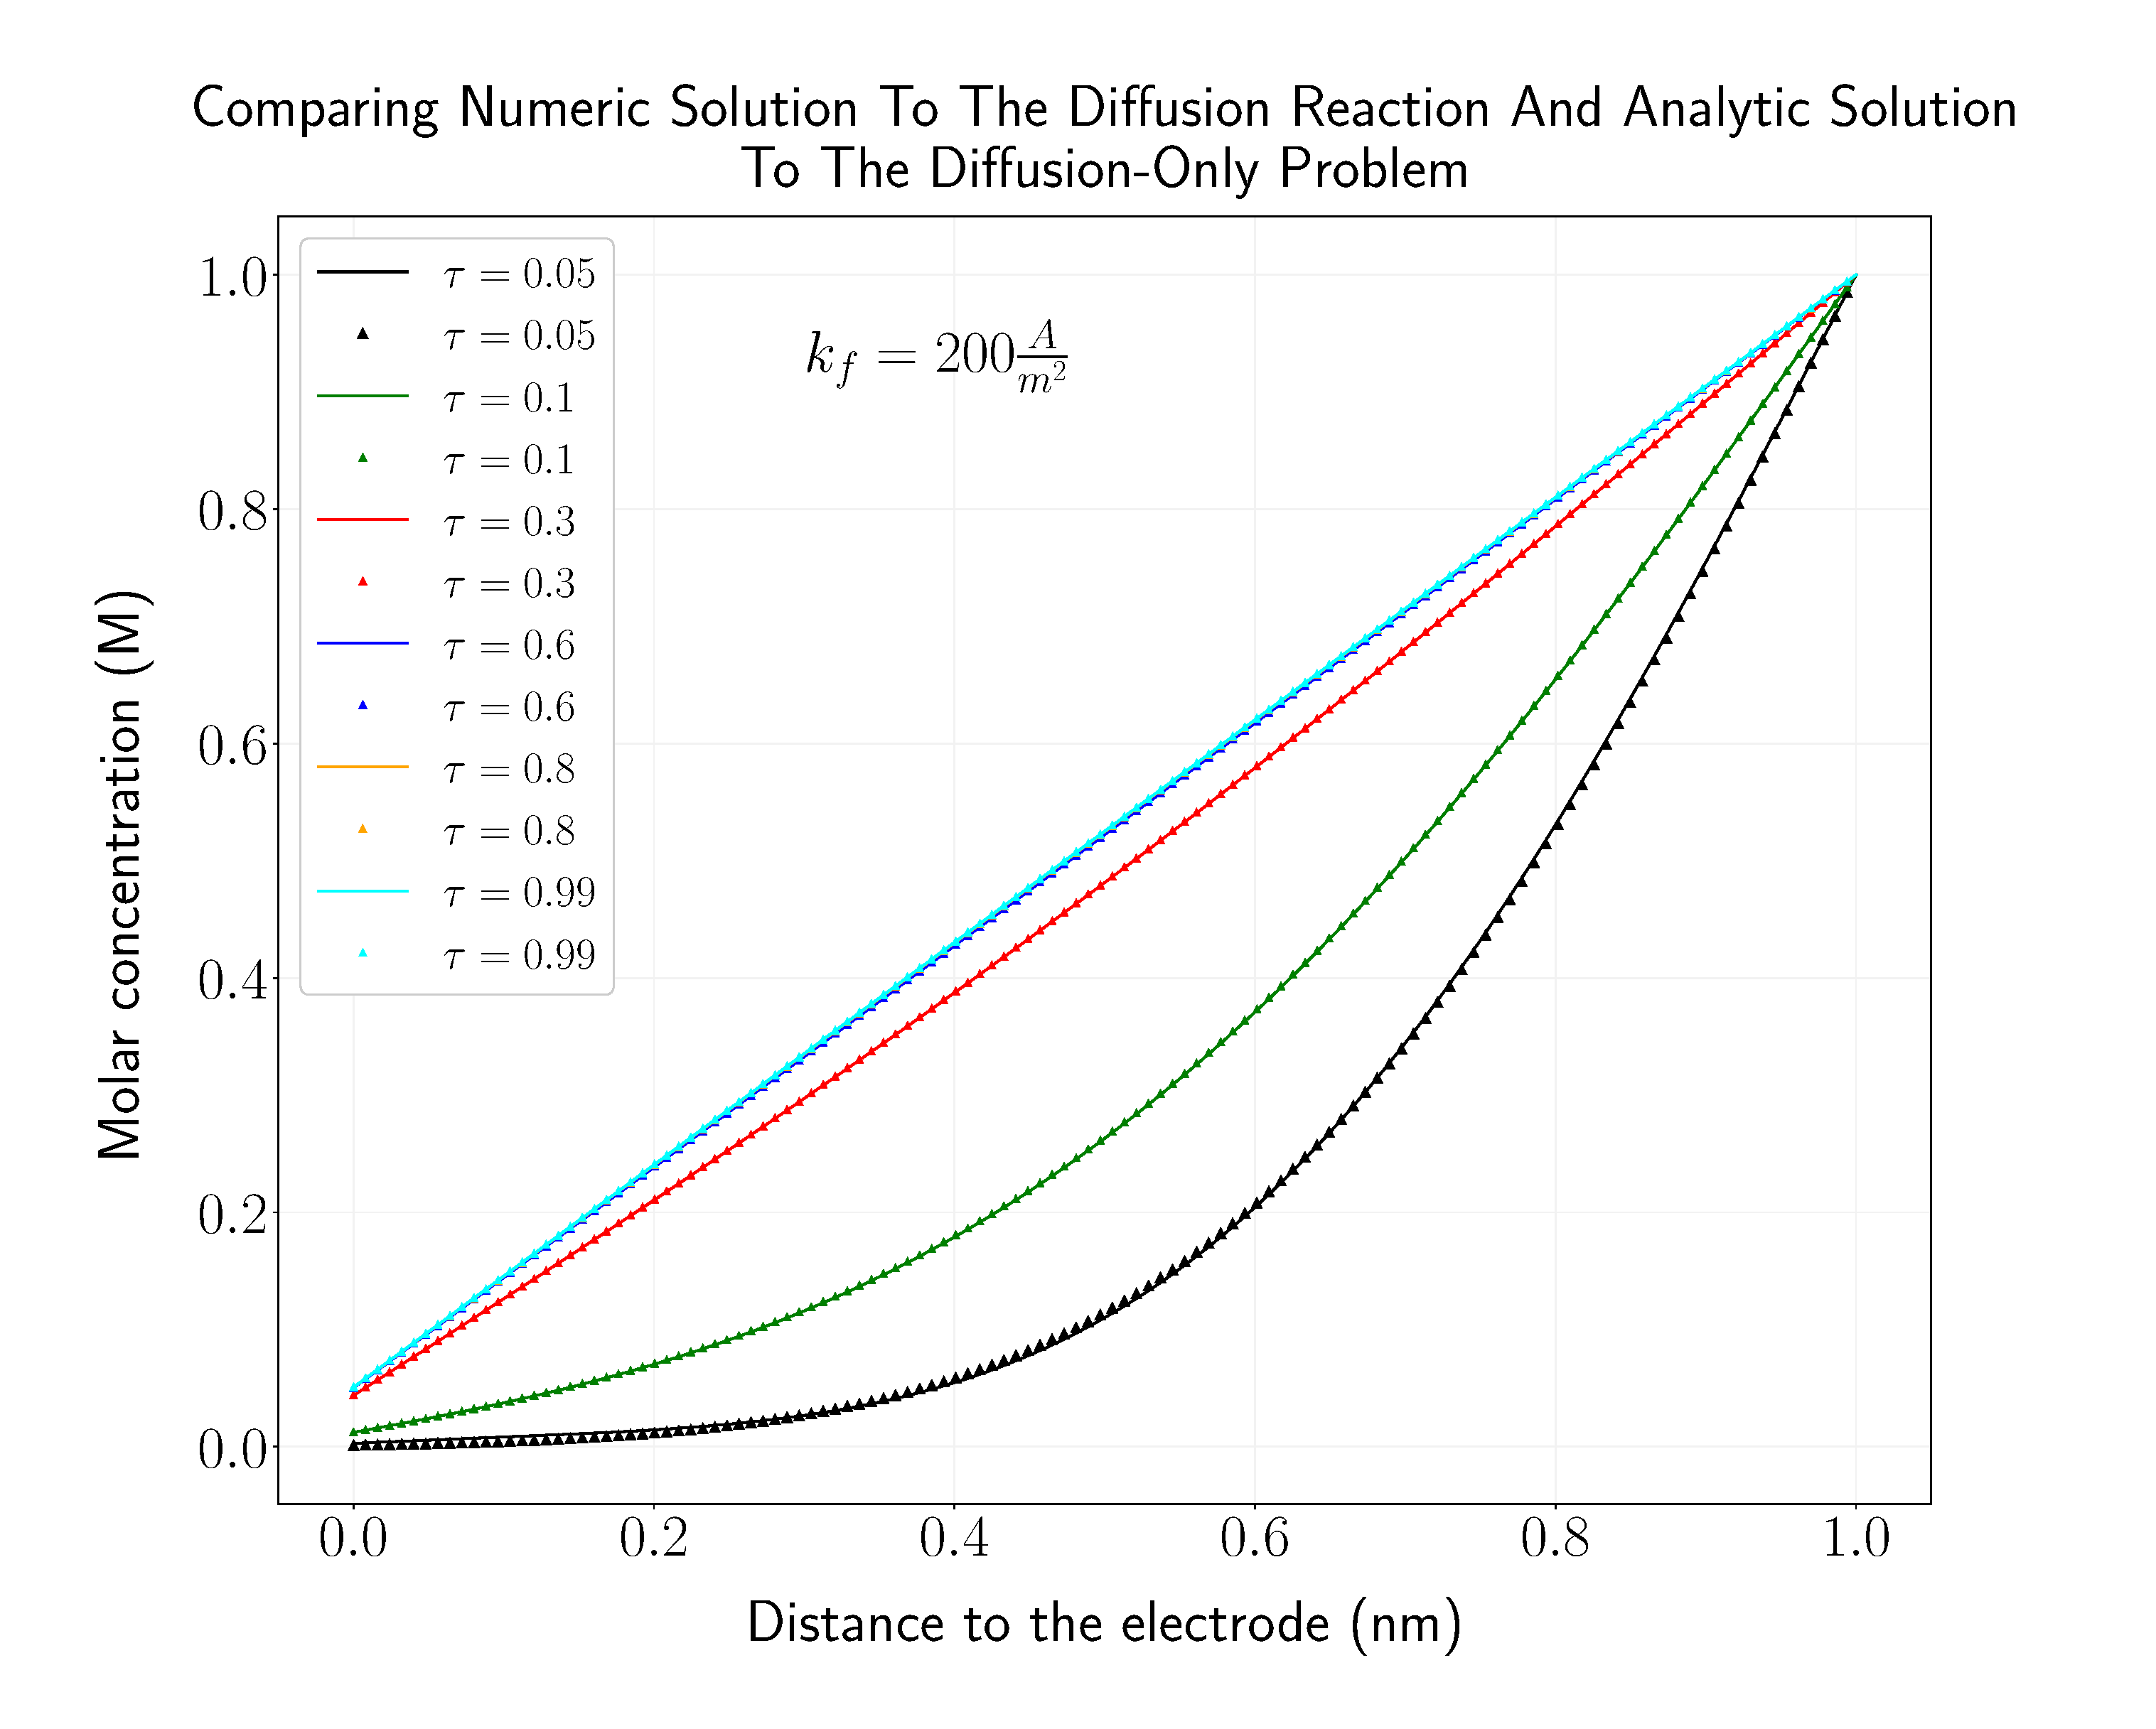
\includegraphics[width=\textwidth]{concentration-diffusion-reaction-robin-comparison}
\caption{In this model, the boundary conditions are physically sensible as the depend on charge carriers to arrive at the interface to produce current. At small $t$ there is no current as copper ions have not reached the surface at $x-0$ and it increases linearly with concentration as time goes on.}
\label{fig:diffusion-reaction-comparison}
\end{figure}


\section{Diffusion-Reaction Equation With Nernst Convection Term.}


The complete dynamic system is given by

\begin{align} \label{eq:diffusion-nernst}
\frac{\partial C_+}{\partial t} &= \mathcal{D_+}\left(\nabla^2 C_+(x) +\nabla \cdot \qty{C_+(x)\qty{\frac{z \mathcal{F}}{RT}\nabla\phi(x)}}\right), \\
\frac{\partial C_-}{\partial t} &= \mathcal{D_-}\left(\nabla^2 C_-(x) -\nabla \cdot \qty{C_-(x)\qty{\frac{z \mathcal{F}}{RT}\nabla\phi(x)}}\right),\\
	\nabla^2 \phi &= \frac{\qty{z\mathcal{F}}}{\epsilon}\qty{C_- - C_+}.
\end{align}

Boundary conditions are fixed by the flux at the interface and boundary conditions at the bulk.

\begin{align}
    J_+(x = 0) &= -\mathcal{D}_+\qty{\frac{\partial C_+}{\partial x} - C_+ \frac{z\mathcal{F}}{RT}\frac{\partial\phi}{\partial x}}\bigg|_{x= 0}= -k_f C_+(x = 0, t),\\
    J_-(x = 0) &= -\mathcal{D}_-\qty{\frac{\partial C_-}{\partial x} + C_- \frac{z\mathcal{F}}{RT}\nabla\phi} \bigg|_{x= 0} = 0,\\
    C_+(\delta) = C_b,\\
    C_-(\delta) = C_b,\\
    \phi(x = 0) &= V_0,\\
    \phi(x = \delta) &= 0.
\end{align}

Initial conditions are given by

\begin{align}
	C_s(x, t=0) = 0,\\
	\phi (x,t=0) = 0.
\end{align}

Let 

\begin{align}
	\Psi(x, t) = \frac{z\mathcal{F}}{RT}\phi(x, t), \\
	\rho_s(x, t) = \frac{C_s(x, t)}{C_b},
\end{align}

be the adimentional potential and adimentional concentration where $s=\pm$ and 

\begin{align}
	\kappa = \sqrt{\frac{\qty{z\mathcal{F}}^2C_b}{\epsilon RT}}.
\end{align}

be the ionic force. Also, we define the adimentional distance parameter $\xi$ and the adimentional time parameter $\tau$ defined as

\begin{align}
	\xi = \kappa x, \\
	\tau = D_+\kappa^2 t
\end{align}

We rewrite equations \ref{eq:diffusion-nernst} as an adimentional system of equations

\begin{align}
\label{eq:adimetional-diffusion-nernst}
    \frac{\partial \rho_+}{\partial \tau} &= \qty{\nabla_\xi^2 \rho_+ - \nabla_\xi\qty{\rho_+ \nabla_\xi \Psi}}, \\
    \frac{\partial \rho_-}{\partial \tau} &= \frac{\mathcal{D}_-}{\mathcal{D_+}}\qty{\nabla_\xi^2 \rho_- + \nabla_\xi\qty{\rho_- \nabla_\xi \Psi}}, \\
    \nabla_\xi^2 \Psi &= \kappa^2\qty{\rho_- - \rho_+}.
\end{align}


In our adimentional units we get

\begin{align}
    J_+(\xi = 0) &= -\mathcal{D}_+\kappa C_+\qty{\frac{\partial \rho_+}{\partial \xi} - \rho_+ \frac{\partial\Psi}{\partial \xi}}\bigg|_{x= 0}= -k_f C_b\rho_s(\xi = 0, \tau)\\
    J_-(\xi = 0) &= -\mathcal{D}_-\kappa C_-\qty{\frac{\partial \rho_-}{\partial \xi} + \rho_- \frac{\partial\Psi}{\partial \xi}}  \bigg|_{x= 0} = 0\\
    \rho_+(\delta) = 1\\
    \rho_-(\delta) = 1\\
    \Psi(\xi = 0) &= \frac{z\mathcal{F}}{RT} V_0 = \Psi_0\\
    \Psi(\xi = \kappa \delta) &= 0
\end{align}

And the adimentional initial conditions are

\begin{align}
	\rho_s(\xi, \tau = 0) = 0,\\
	\Psi (\xi, \tau = 0) = 0.
\end{align}


\subsection{Discrete equations}

In order to obtain the numerical solution of our system, we need to discretize equations \ref{eq:diffusion-nernst}. For each species ($s = \pm$) we have

\begin{align}
    \rho_s^{n+1, k} =& \rho_s^{n,k} \qty{1 - 2 \alpha_s + s \alpha_s \qty{\Psi^{n, k} - \Psi^{n, k-1}}} \\ & + \alpha_s \rho_s^{n, k+1} \qty{1 - s \qty{\Psi^{n,k+1} - \Psi^{n,k}}} + \alpha_s \rho_s^{n,k-1},\\
    \Psi^{n+1, k+1} - 2\Psi^{n+1,k} + \Psi^{n+1, k-1} =& \Delta \xi^2 \qty{C_+^{n+1, k} - C_-^{n+1, k}}.
\end{align}

where we have defined 

\begin{eqnarray*}
	\alpha_+ = \frac{\Delta \tau}{\Delta \xi^2}\\
	\alpha_- = \frac{\Delta \tau}{\Delta \xi^2}\frac{\mathcal{D}_-}{\mathcal{D}_+}.
\end{eqnarray*}
Boundary conditions need to be discretized accordingly

\begin{align}
\rho_s^{n+1, 0} &= \gamma_s \rho_s^{n+1, 1},\\
\rho_s^{n+1, M} &= 1,\\
\Psi^{n+1, 0} &= \Psi_0,\\
\Psi^{n+1, M} &= 0,\\
\Psi^{n+1, M} &= \Psi^{n+1, M-1} .
\end{align}


with

\begin{align}
\gamma_+ &= \frac{1}{1 + \frac{\Delta \xi}{\mathcal{D}_+}\frac{k_f}{\kappa} + \qty{\Psi^{n+1, 1}-\Psi^{n+1,0}} }, \\
\gamma_- &= \frac{1}{1 - \qty{\Psi^{n+1, 1}-\Psi^{n+1,0}} }
\end{align}

This equations yield the following boundary equations

$$ k=1 $$

\begin{align}
    \rho_s^{n+1, 1} = \rho_s^{n,1} \qty{1 - 2 \alpha_s + \alpha_s \gamma_s + s \alpha_s \qty{\Psi^{n, 1} - \Psi^{n, 0}}} + \alpha_s \rho_s^{n, 2} \qty{1 - s \qty{\Psi^{n,2} - \Psi^{n,1}}},\\
    \Psi^{n+1, 2} - 2\Psi^{n+1,1} + \Psi^{n+1, 0} =& \Delta \xi^2\qty{C_+^{n+1, 1} - C_-^{n+1, 1}}.
\end{align}


$$ k = m-1 $$

\begin{align}
    \rho_s^{n+1, m-1} = \rho_s^{n,m-1} \qty{1 - 2 \alpha_s + s \alpha_s \qty{\Psi^{n, m-1} - \Psi^{n, m-2}}} + \alpha_s \rho_s^{n, m} \qty{1 - s \qty{\Psi^{n,m} - \Psi^{n,m-1}}},\\
    \Psi^{n+1, 2} - 2\Psi^{n+1,1} + \Psi^{n+1, 0} = \Delta \xi^2 \qty{C_+^{n+1, 1} - C_-^{n+1, 1}}.  
\end{align}

\subsection{Matrix equations}

We can write the system as follows

\begin{align}
\underline{\rho_s^{n+1}} = (\bf{A} + s\alpha_s\bf{B}(\Psi^{n}) ) \cdot \underline{\rho_s^{n}} + \bf{b_s},\\
\bf{D} \underline{\Psi}^{n+1} = \Delta \xi ^2\qty{\underline{C_-}^{n+1} - \underline{C_+}^{n+1}}- \underline{b}_{\Psi}.
\end{align}


where

\begin{align}
A = \begin{bmatrix}
    1 - 2 \alpha_s + \alpha_s \gamma_s   &  \alpha_s   & 0  &   \cdots & 0   &   0   &   0   &   0 \\
    \alpha_s    &   1 - 2 \alpha_s       &  \alpha_s   & 0  & \cdots   & 0   &   0   &   0 \\
    0         & \alpha_s               &  1 - 2 \alpha_s  & \alpha_s   & \cdots   &   0   &   0   &   0 \\
    \vdots    &  \vdots              &\vdots          &  \vdots  & \vdots   &\vdots & \vdots & \vdots \\ 
    0         &  0                   &  \cdots        &  0       &  \alpha_s    &  1-2\alpha_s &    \alpha_s   &    0 \\
0         &  0                   &  \cdots        &  0           &  0         &     0      &  \alpha_s    &  1-2\alpha_s 
\end{bmatrix},
\end{align}


\begin{align}
B(\Psi) = \begin{bmatrix}
    \qty{\Psi^{n,1} - \Psi^{n, 0}}   &  -\qty{\Psi^{n,2} - \Psi^{n, 1}}   & 0  &   \cdots   0   &   0   &   0 \\
    0                                &  \qty{\Psi^{n,1} - \Psi^{n, 0}}    & -\qty{\Psi^{n,2} - \Psi^{n, 1}}   & 0  & \cdots    &   0 \\
    \vdots    &  \vdots              &\vdots           &\vdots & \vdots & \vdots \\ 
    0         &  0                   &  \cdots        &  0              & \qty{\Psi^{n,M-2} - \Psi^{n, M-3}}   & -\qty{\Psi^{n,M-1} - \Psi^{n, M-2}} \\
0         &  0                   &  \cdots              &     0      &  0    &  \qty{\Psi^{n,M-1} - \Psi^{n, M-2}}
\end{bmatrix}.
\end{align}

Also, 
\begin{align}
D = \begin{bmatrix}
    -2   &  1   & 0  &   \cdots & 0   &   0   &   0   &   0 \\
    1    &  -2    & 1   & 0  & \cdots   & 0   &   0   &   0 \\
    0         & 1                    &  -2   & 1 & \cdots    &   0   &   0 \\
    \vdots    &  \vdots              &\vdots          &  \vdots  & \vdots   &\vdots & \vdots & \vdots \\ 
    0         &  0                   &  \cdots        &  0       &  0         &  0         & -2   & 1 \\
0         &  0                   &  \cdots        &  0           &  0         &     0      &  1    &  -2
\end{bmatrix},
\end{align}

\begin{align}
    b_\Psi = \begin{bmatrix}
        \Psi_0\\
        0\\
        \vdots\\
        0
    \end{bmatrix},
\end{align}

\begin{align}
    b_s = \begin{bmatrix}
        0\\
        0\\
        \vdots\\
        0\\
        1\end{bmatrix}.
\end{align}



\begin{figure}[htbp]
\centering
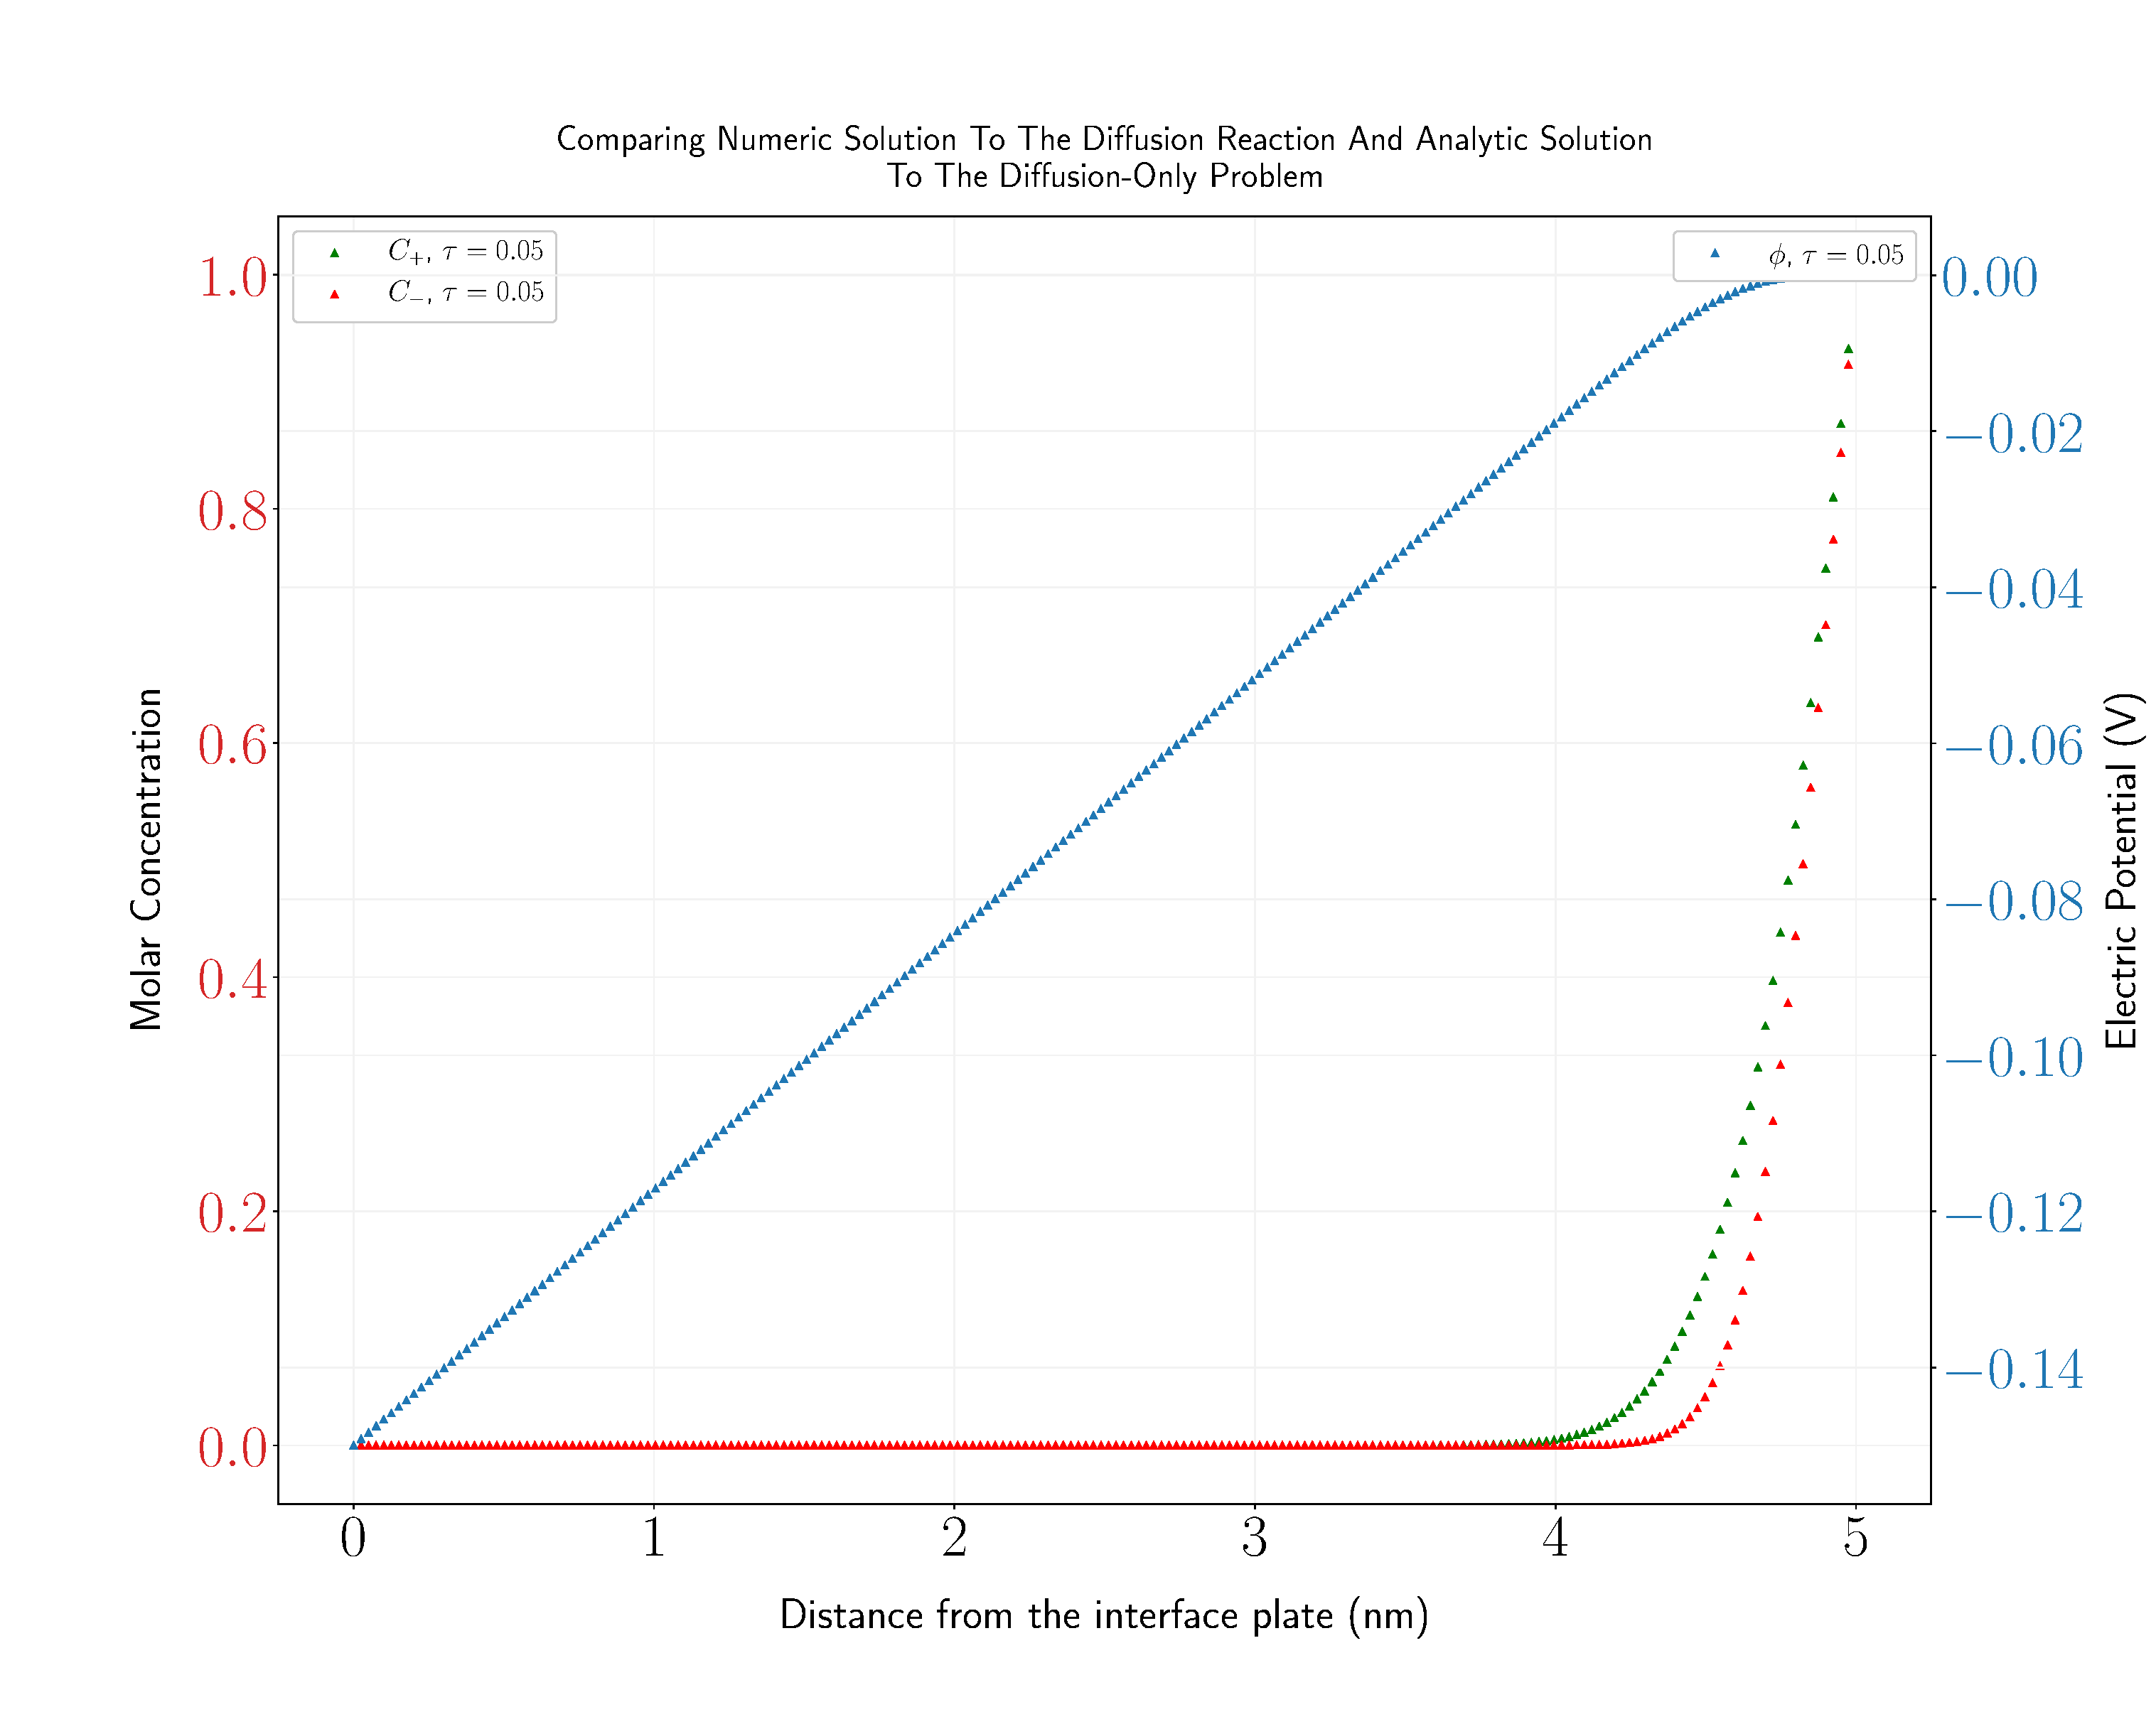
\includegraphics[width=\textwidth]{complete-diffusion-nernst.eps}
\caption{Numerical solution to system \ref{eq:diffusion-nernst}. Red and green dots represent the negative ($SO_4^{-2}$ and positive $Cu^{+2}$ electrolyte concentrations respectively (left axis). The blue dots represent the electric potential (right axis).}
\label{fig:diffusion-comparison}
\end{figure}










%\section{Forced Current Setup}

In the previous section we used a concentration dependent boundary condition. That means that the current is a consequence of the chemical reaction at the interface. In this section we would like force the current. The flux at the interface is defined as

\begin{align}
	\label{eq:forced-current-boundary}
    J_+(x = 0) &= -\mathcal{D}_+\qty{\frac{\partial C_+}{\partial x} - C_+ \frac{z\mathcal{F}}{RT}\frac{\partial\phi}{\partial x}}\bigg|_{x= 0}= R,\\
    J_-(x = 0) &= -\mathcal{D}_-\qty{\frac{\partial C_-}{\partial x} + C_- \frac{z\mathcal{F}}{RT}\nabla\phi} \bigg|_{x= 0} = 0,\\
\end{align}

since only the positive electrolyte reacts with the electrode. The chemical reaction can be written in terms of the concentration as

\begin{align}
	R = -k_f C(t, x=0) = \frac{i_0}{\mathcal{F}},
\end{align}

where $k_f$ is the ......, $i_0$ is the current density (current by unit area) and $\mathcal{F}=N_A e$ the Faraday constant.

Discretizing boundary condition \ref{eq:forced-current-boundary} and letting $C_s = C_b\rho_s$ we get

\begin{align}
	\rho_+^{n,k}=\frac{\rho_+^{n,k+1}-R\Delta \xi/\mathcal{D_+}Cb}{1+\qty{\psi^{n,k+1}-\psi^{n,k}}},\\
	\rho_-^{n,k}=\frac{\rho_-^{n,k+1}}{1-\qty{\psi^{n,k+1}-\psi^{n,k}}},
\end{align}

surfaceDeltaE

forced-current-nernst


\chapter{Results and analysis}
In this chapter we review the results obtained through out this work and obtain phyisicaly relevant quantities from our simulations and analytical computations. 

Throughout this work we have explored three different setups. Firstly we explored the case where there is no chemical reaction at the interface. This is the case of normal electrolytes under no external electric field. Secondly we studied the case where current is imposed through the electrolyte solution and therefore reaction is driven by this current. 

Lastly we studied the case where the reaction takes the form of Langmuir isotherm in the limiting case where the constant $K_{eq}S_T << 1$. 

An interesting parameter extractable from our models is the relaxation time, or the time it takes the system to reach steady state. Also we are interested in finding how the electric field at the surface varies with bulk concentrations and the electrolytic cell's potential.  We'll first analyze steady state solutions and then we'll move on to the dynamical system.



\section{Comparing Numeric An Analytic Results In Steady State Regime}

Fig. \ref{fig:comparison} shows the comparison between the numeric and analytic results. This results are obtained by numerically evaluation system of equations \ref{eq:nernst-planck} and perturvatively finding solutions up to first order on a forced current setup as shown in \ref{eq:first-order-system}



\begin{figure}[htbp]
\begin{subfigure}{.5\linewidth}
\centering
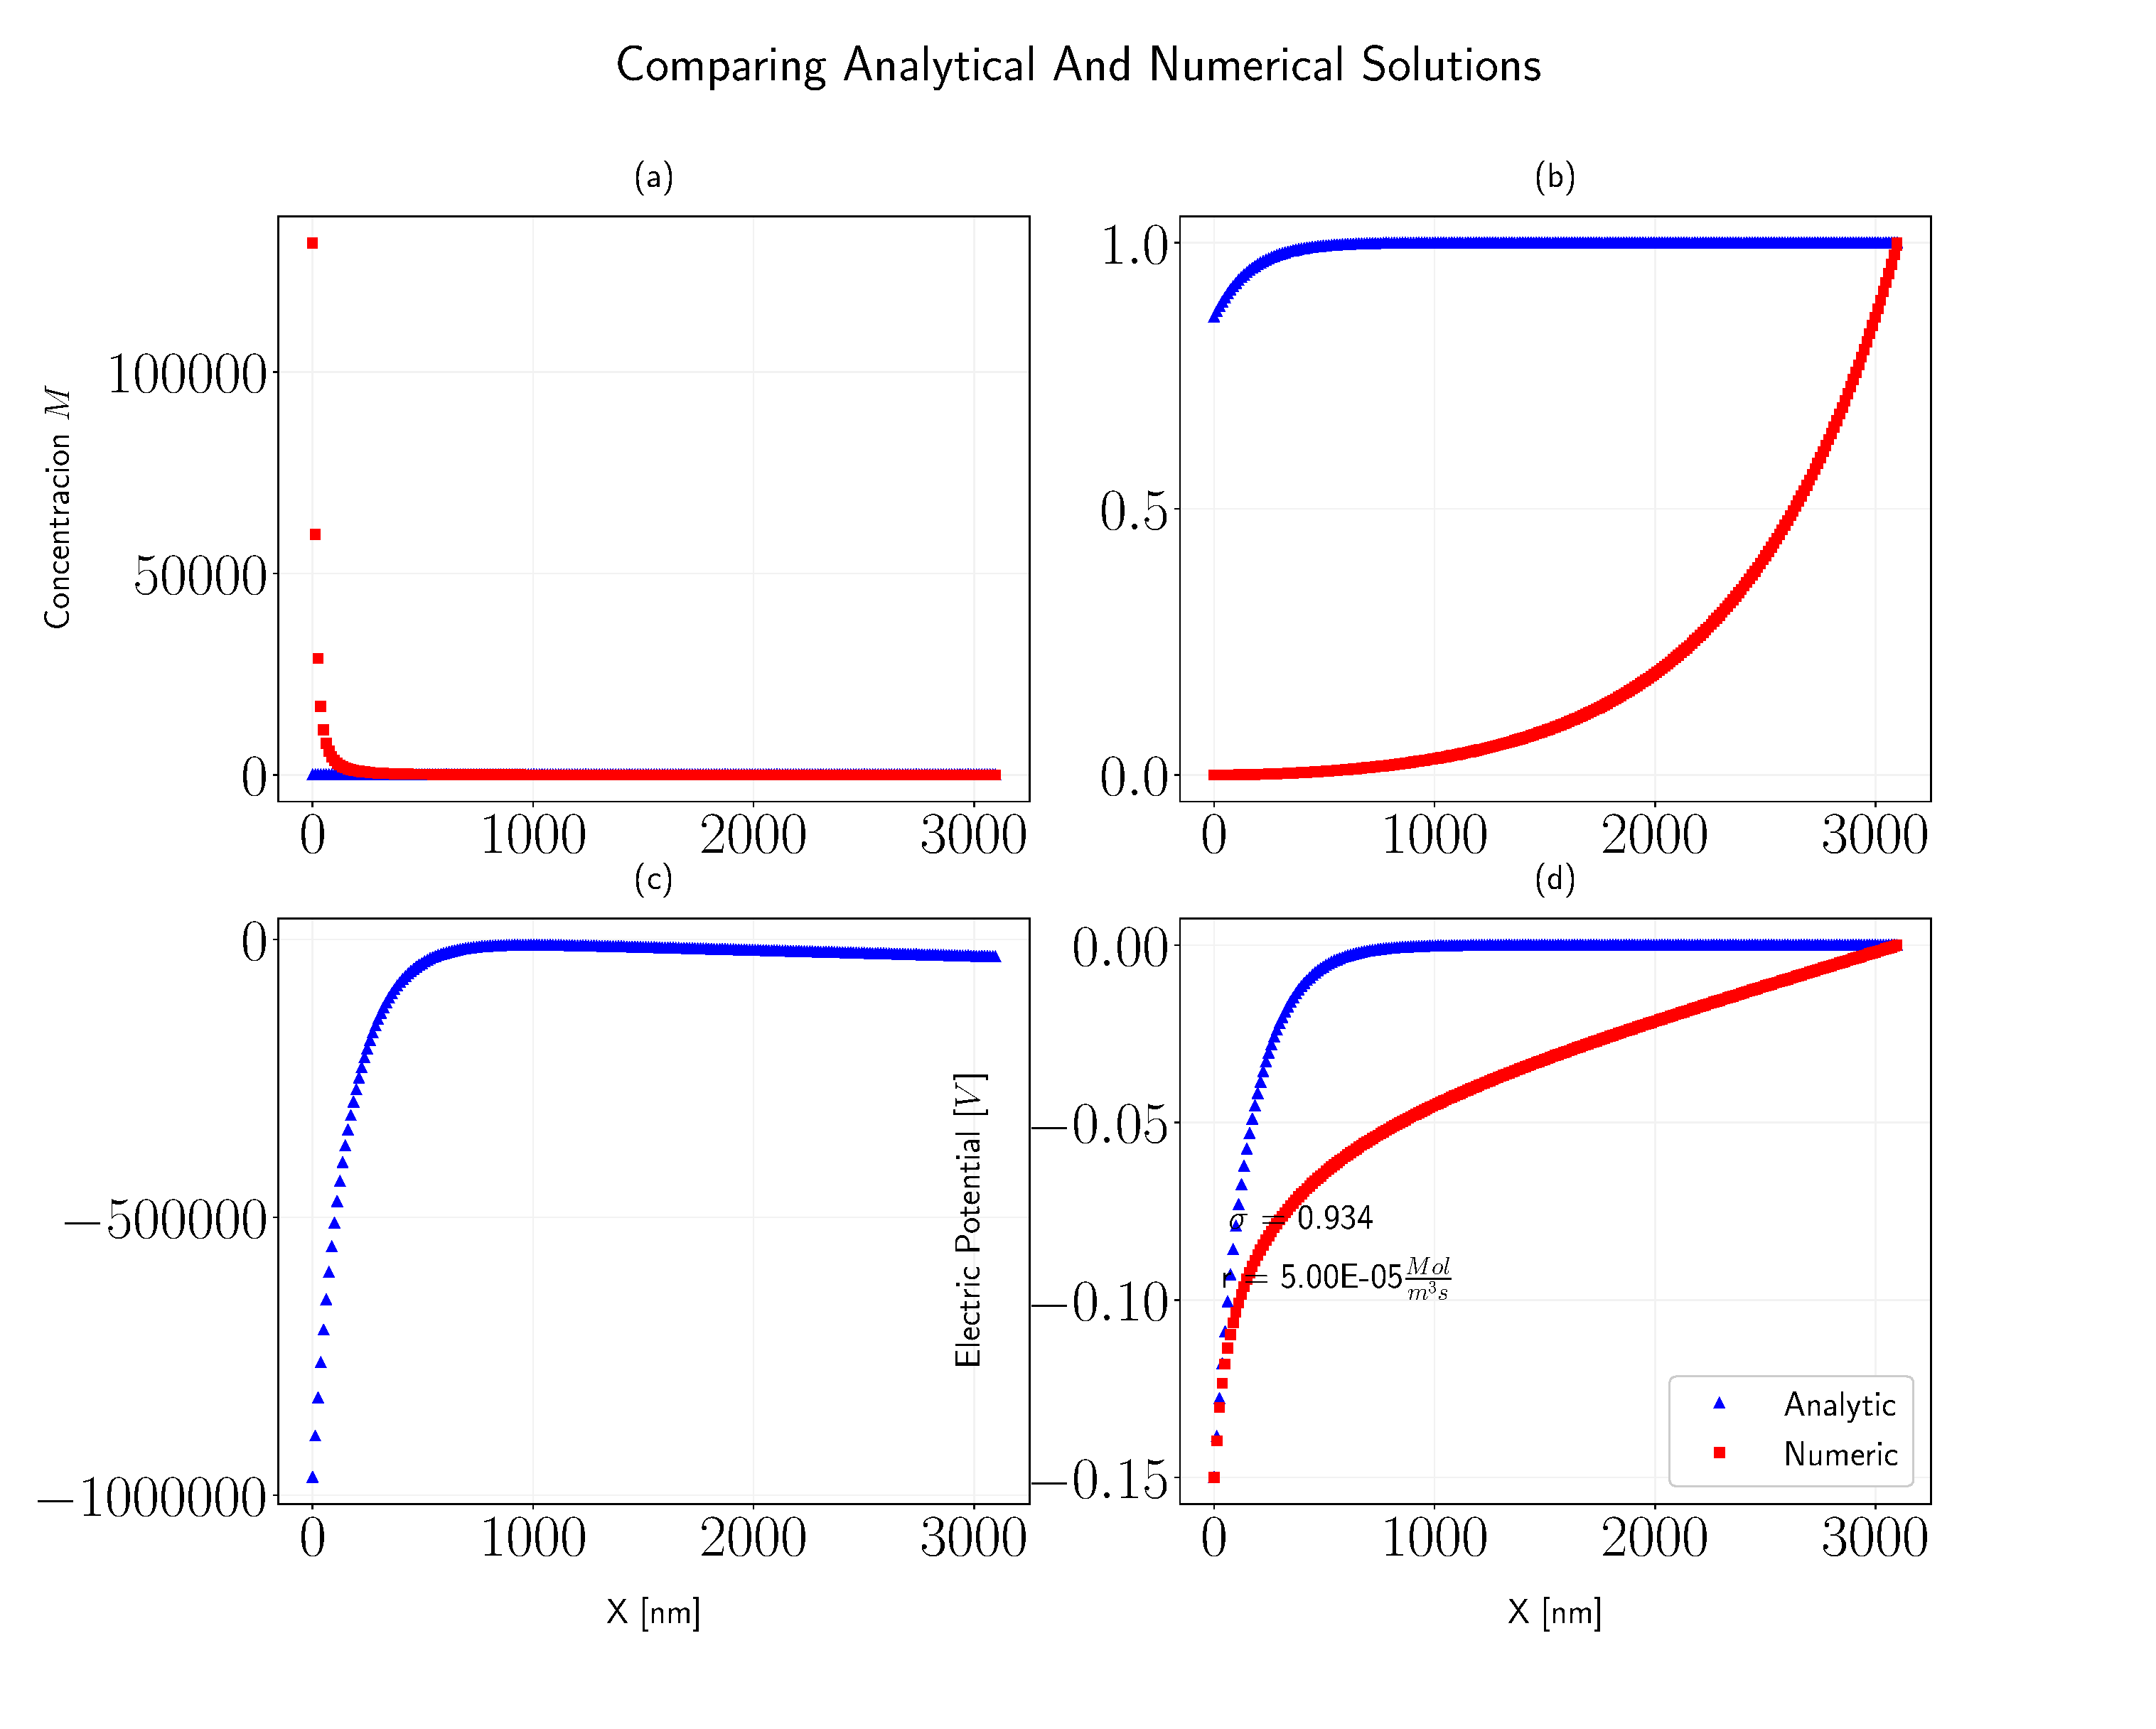
\includegraphics[width=\textwidth]{comparison0}
\caption{}
\label{fig:sub1}
\end{subfigure}%
\begin{subfigure}{.5\linewidth}
\centering
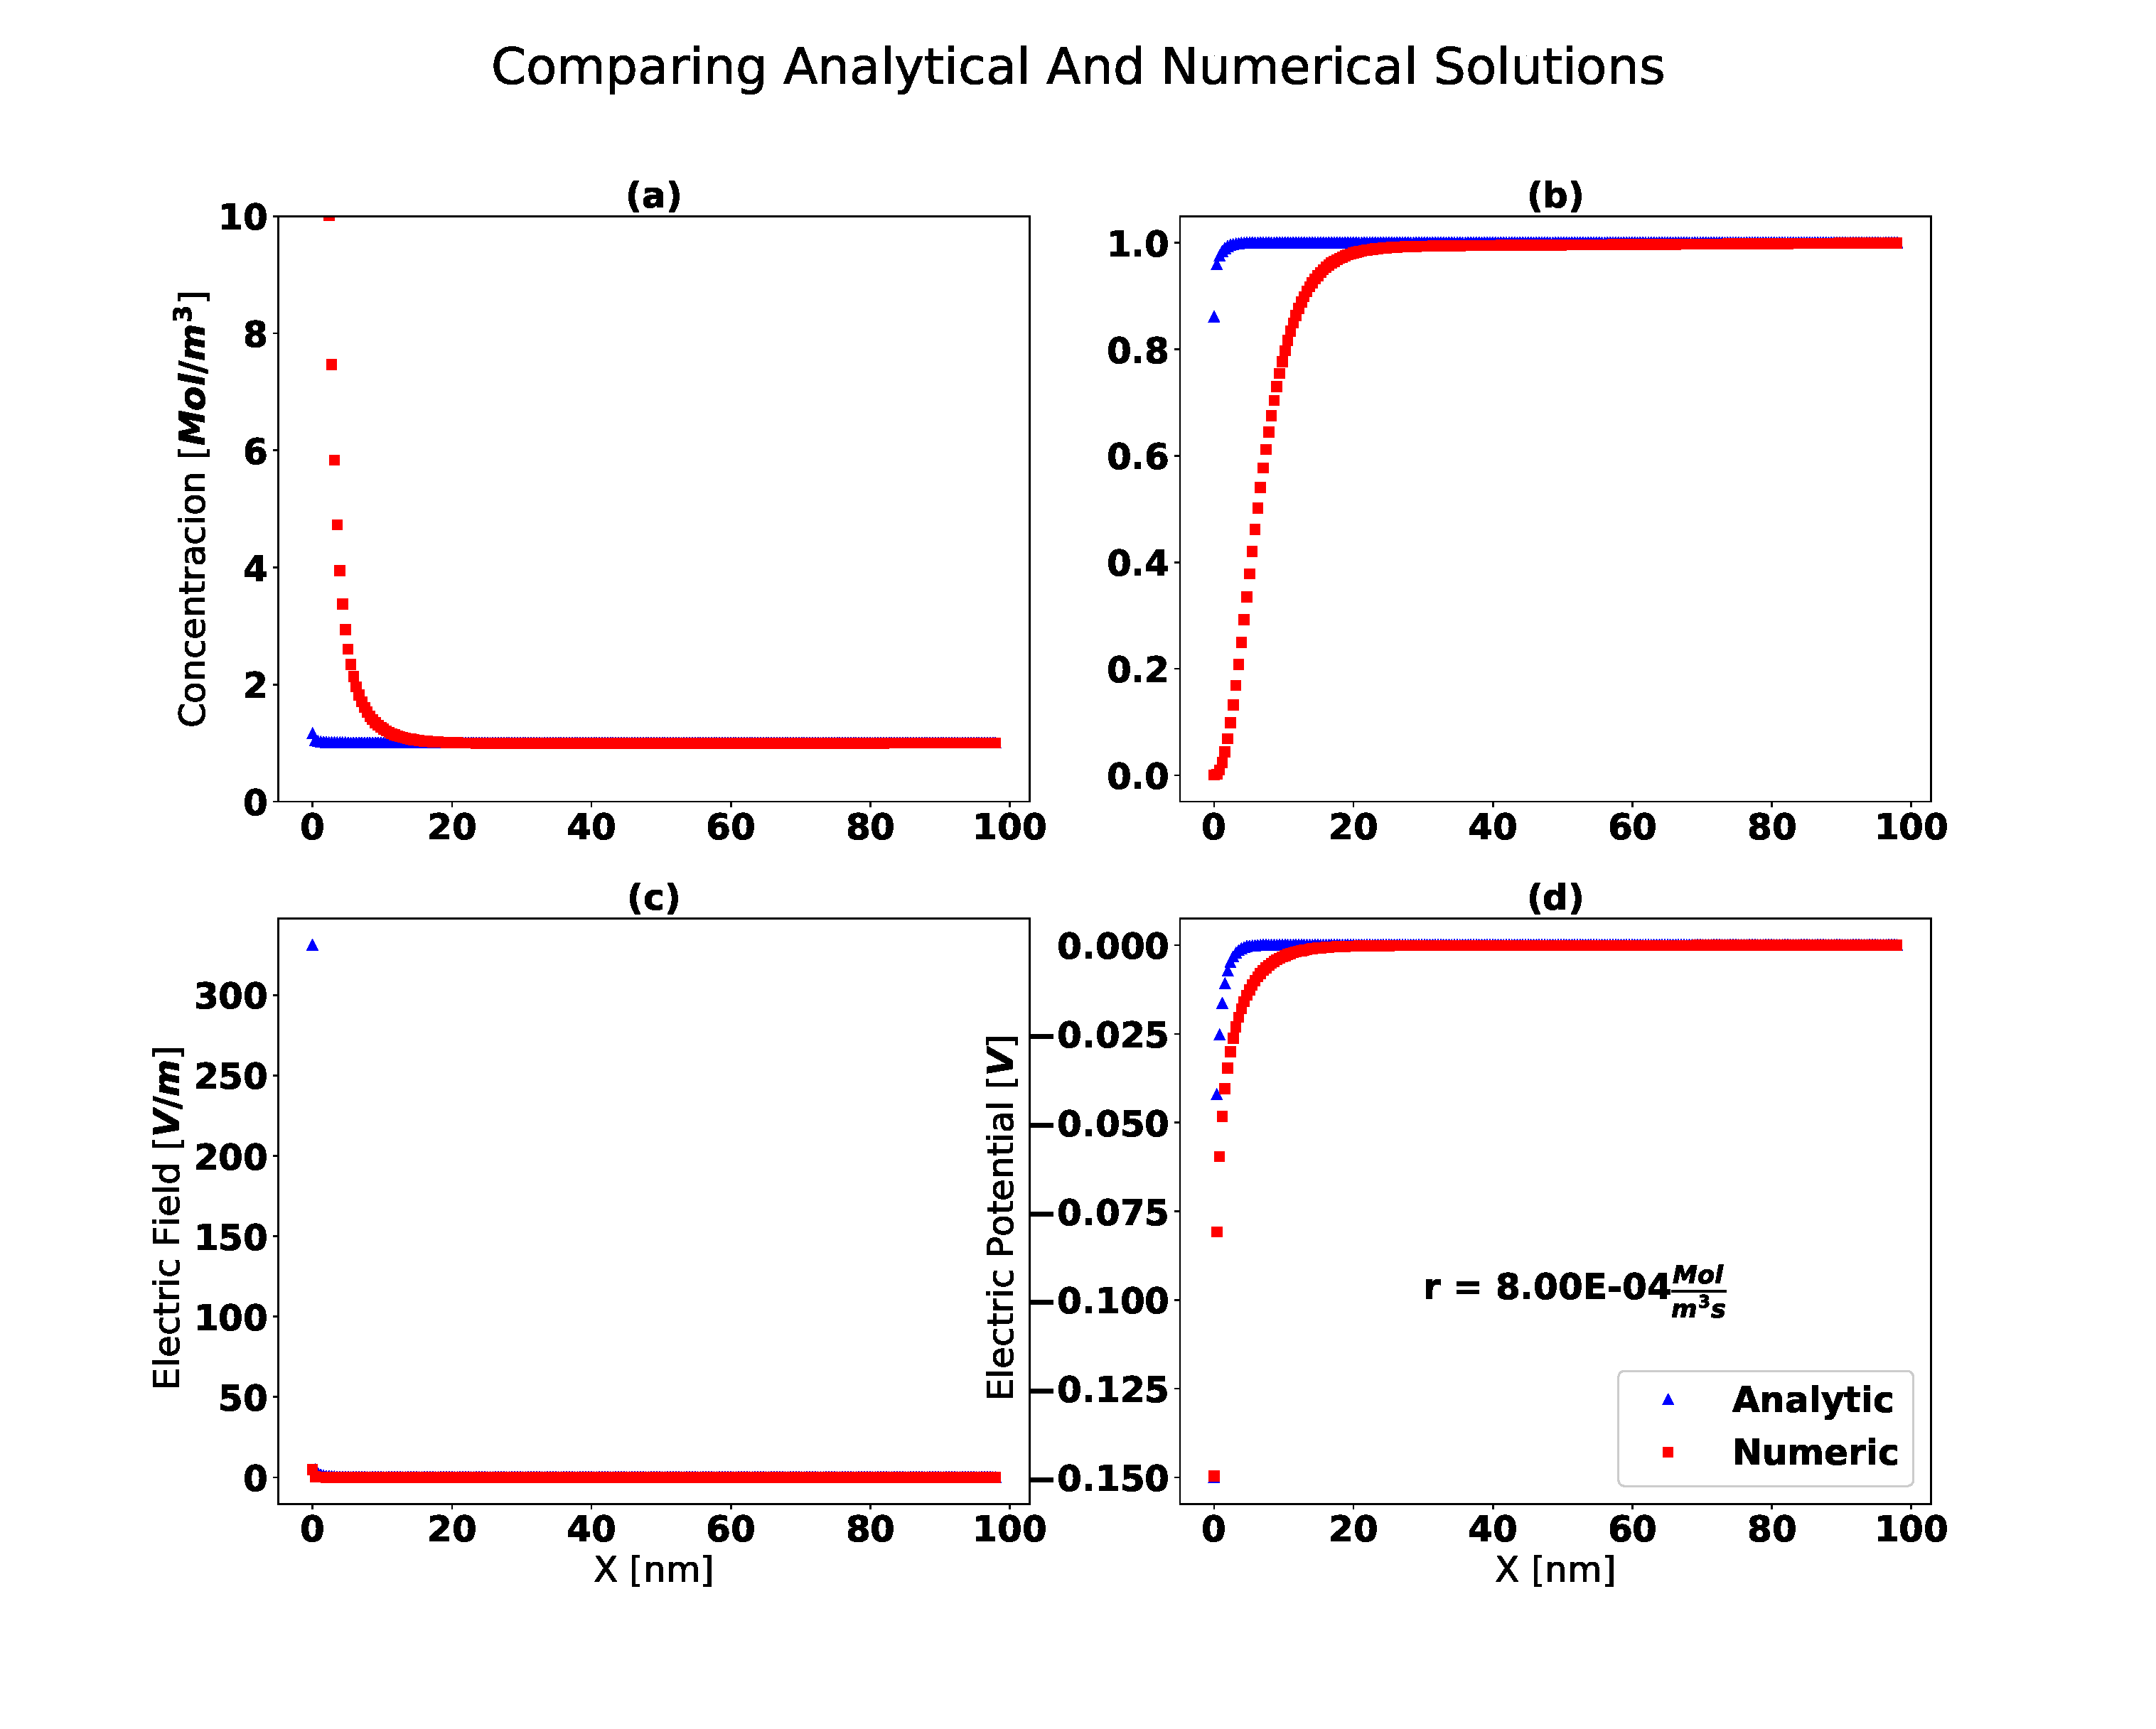
\includegraphics[width =\textwidth]{comparison1}
\caption{}
\label{fig:sub2}
\end{subfigure}\\[1ex]
\begin{subfigure}{\linewidth}
\centering
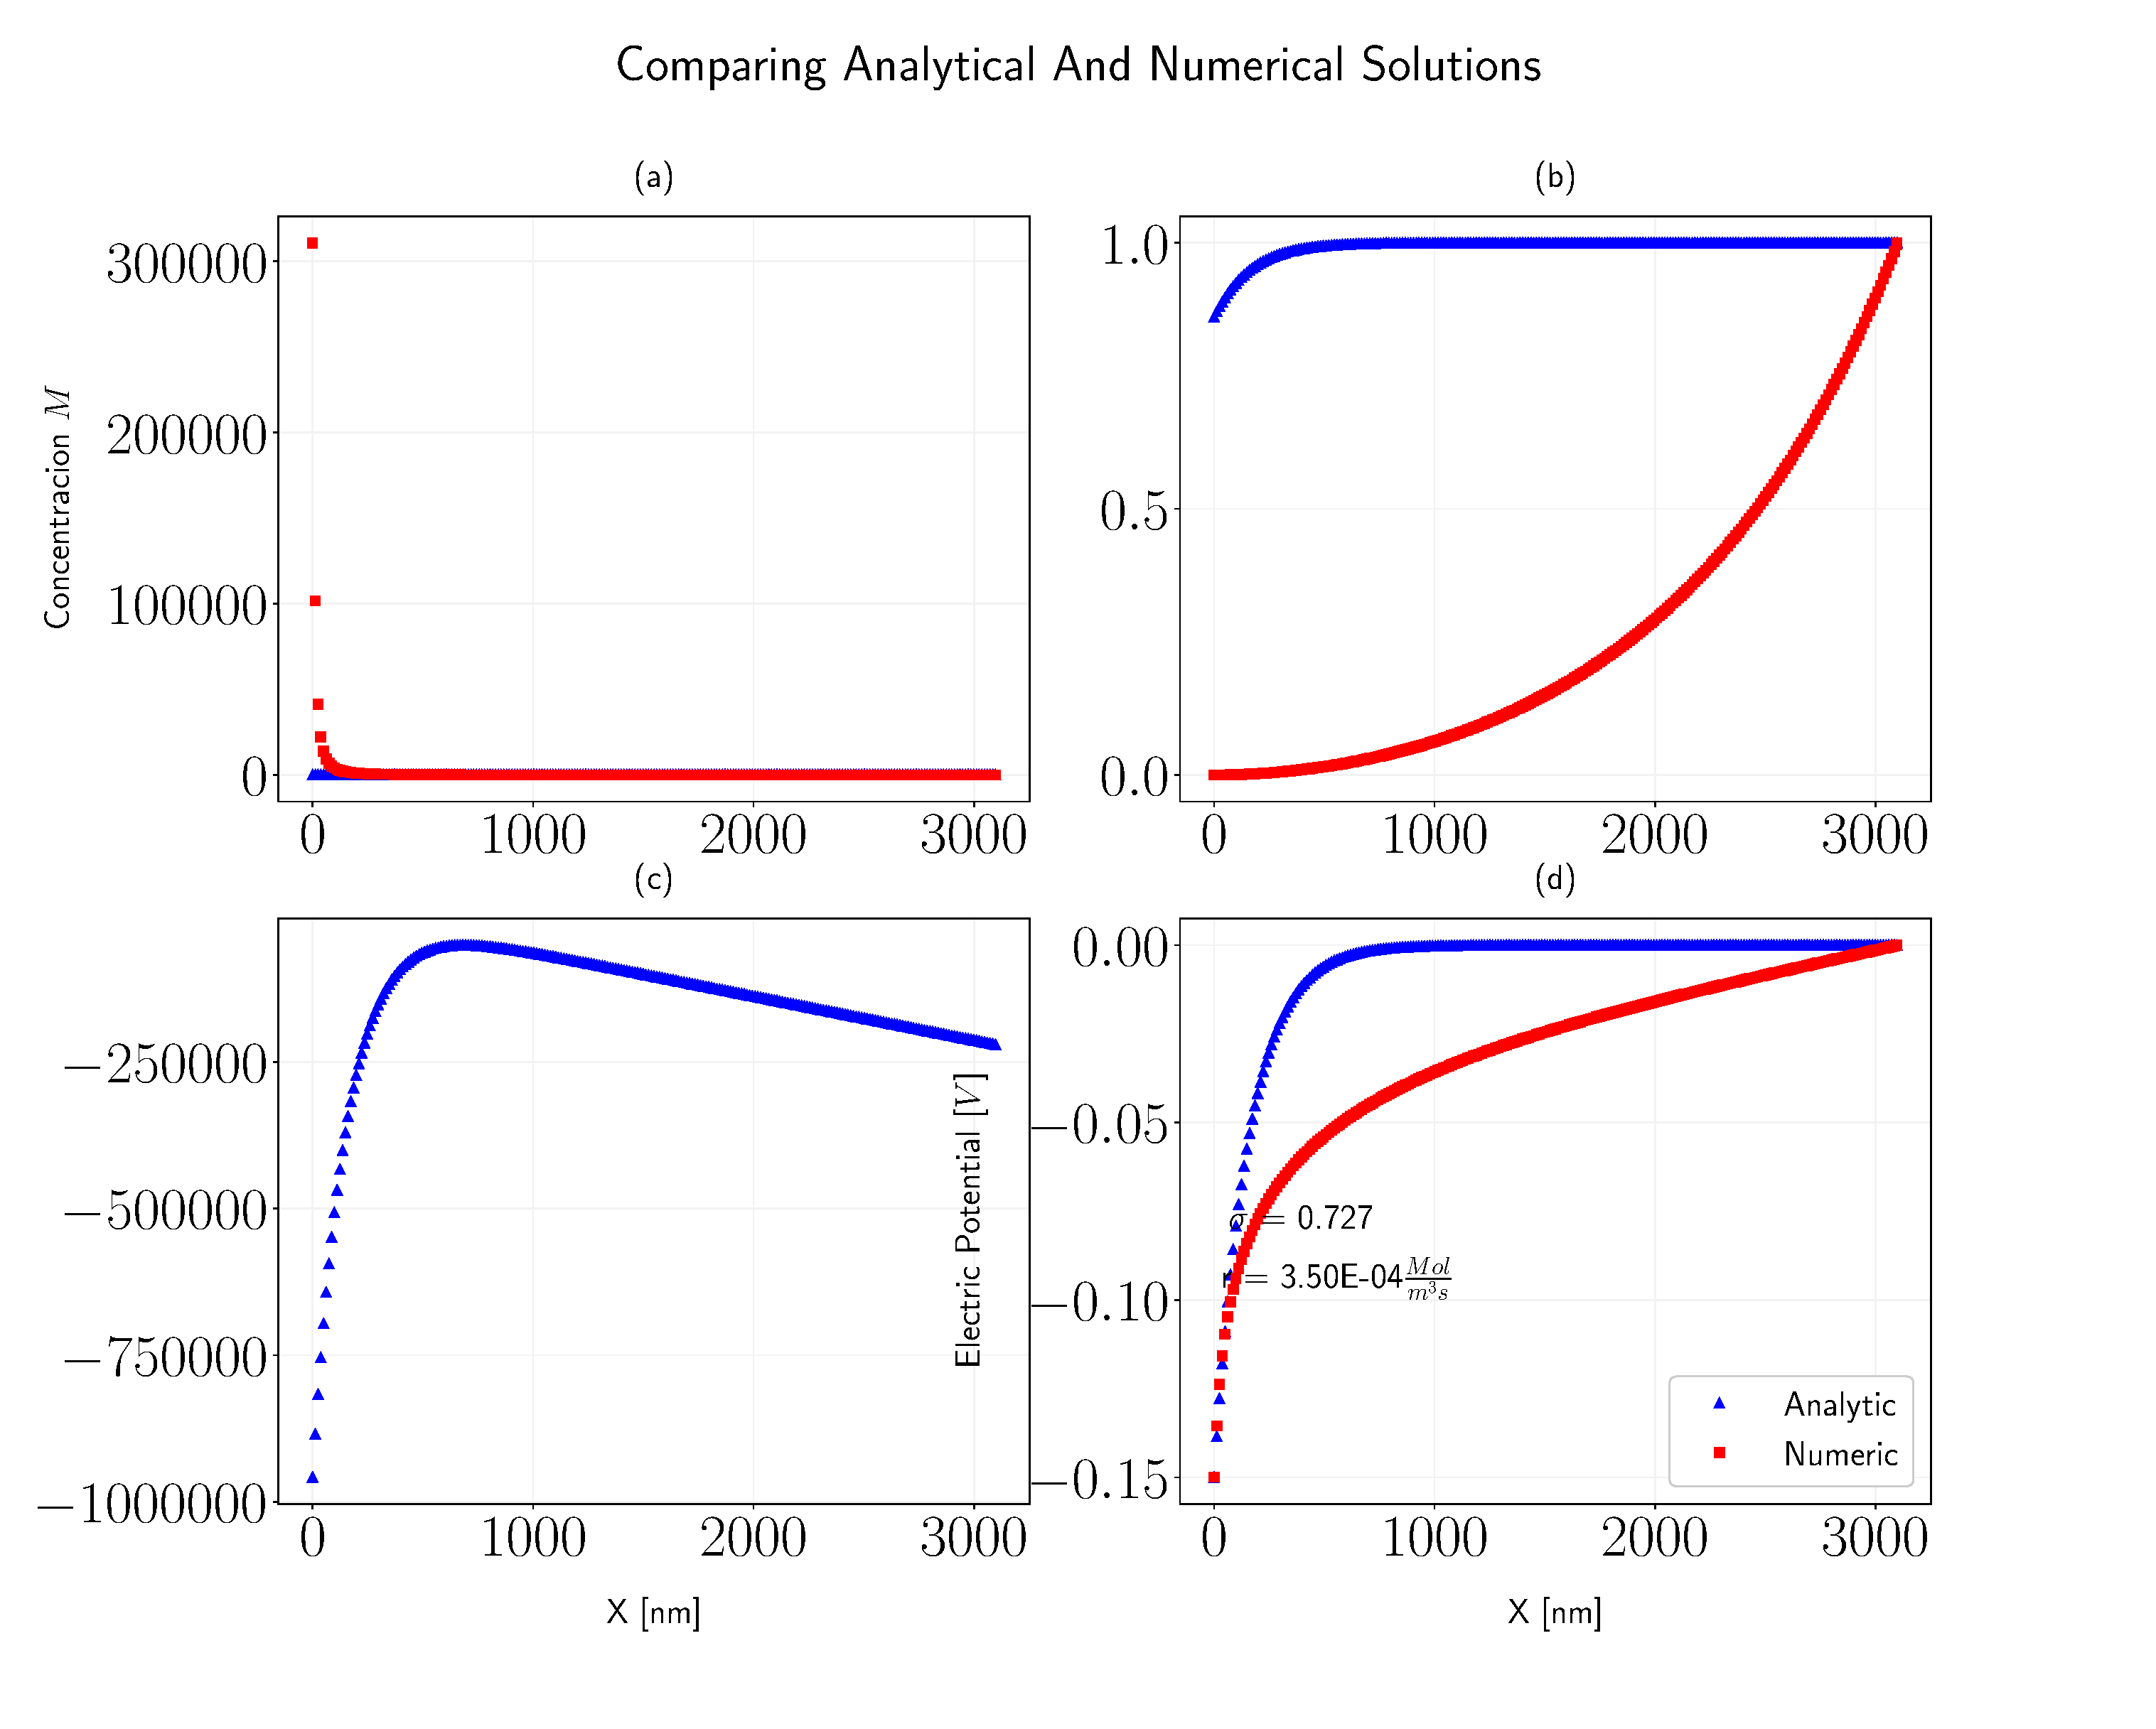
\includegraphics[width =0.5\textwidth]{comparison2}
\caption{}
\label{fig:sub3}
\end{subfigure}
\caption{Three subfigures}
\label{fig:comparison}
\end{figure}



\newpage
\section{Concentration Dependent Boundary Condition}
\subsection{Time evolution}

In this chapter we discus the results obtained by the dynamic algorithm. We study different parameter regimes and the behaviour of the electric potential and electric field.

We are interested in studying the time evolution of the system from initial conditions. Figure \ref{fig:ef1} shows the time evolution of the system for a time window of $t = 4.48 ns$




\begin{figure}[htbp]
\centering
\textbf{Electric Field In The Diffusion Problem With Nernst Interaction.}\par\medskip
\begin{subfigure}{.5\linewidth}
\centering
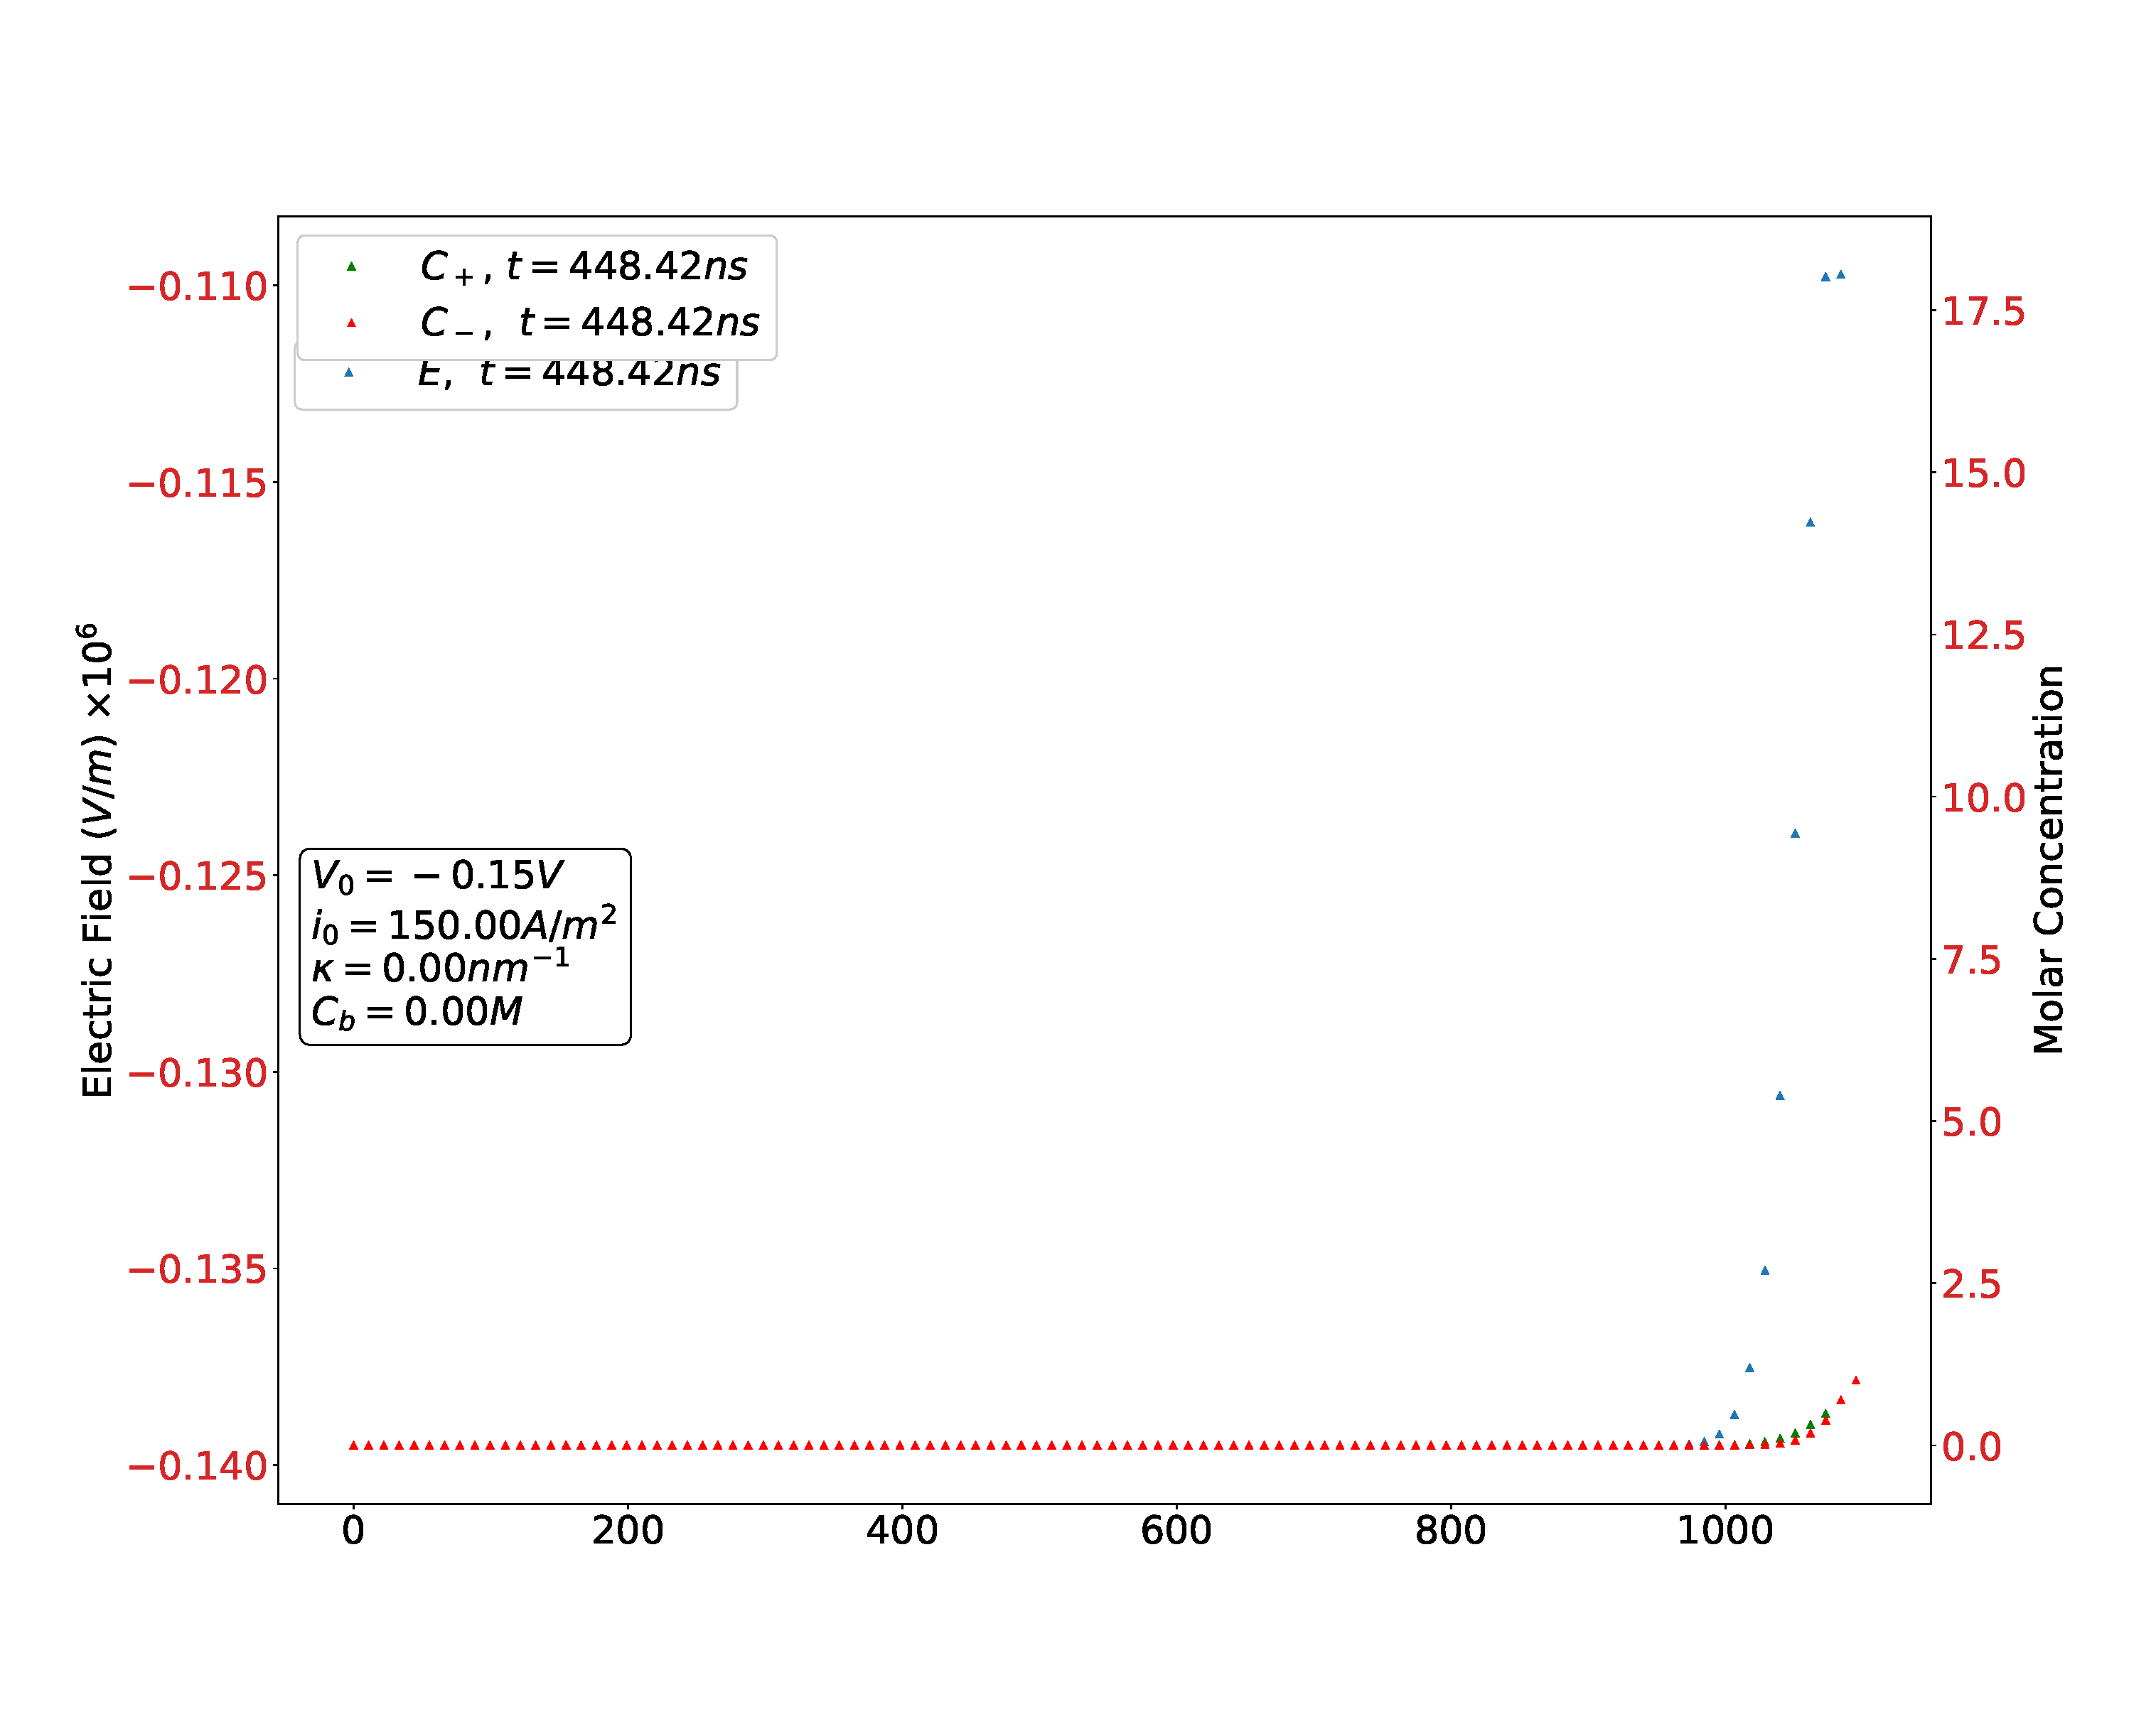
\includegraphics[width=\textwidth]{complete-diffusion-nernstE0.eps}
\caption{}
\label{fig:ef1}
\end{subfigure}%
\begin{subfigure}{.5\linewidth}
\centering
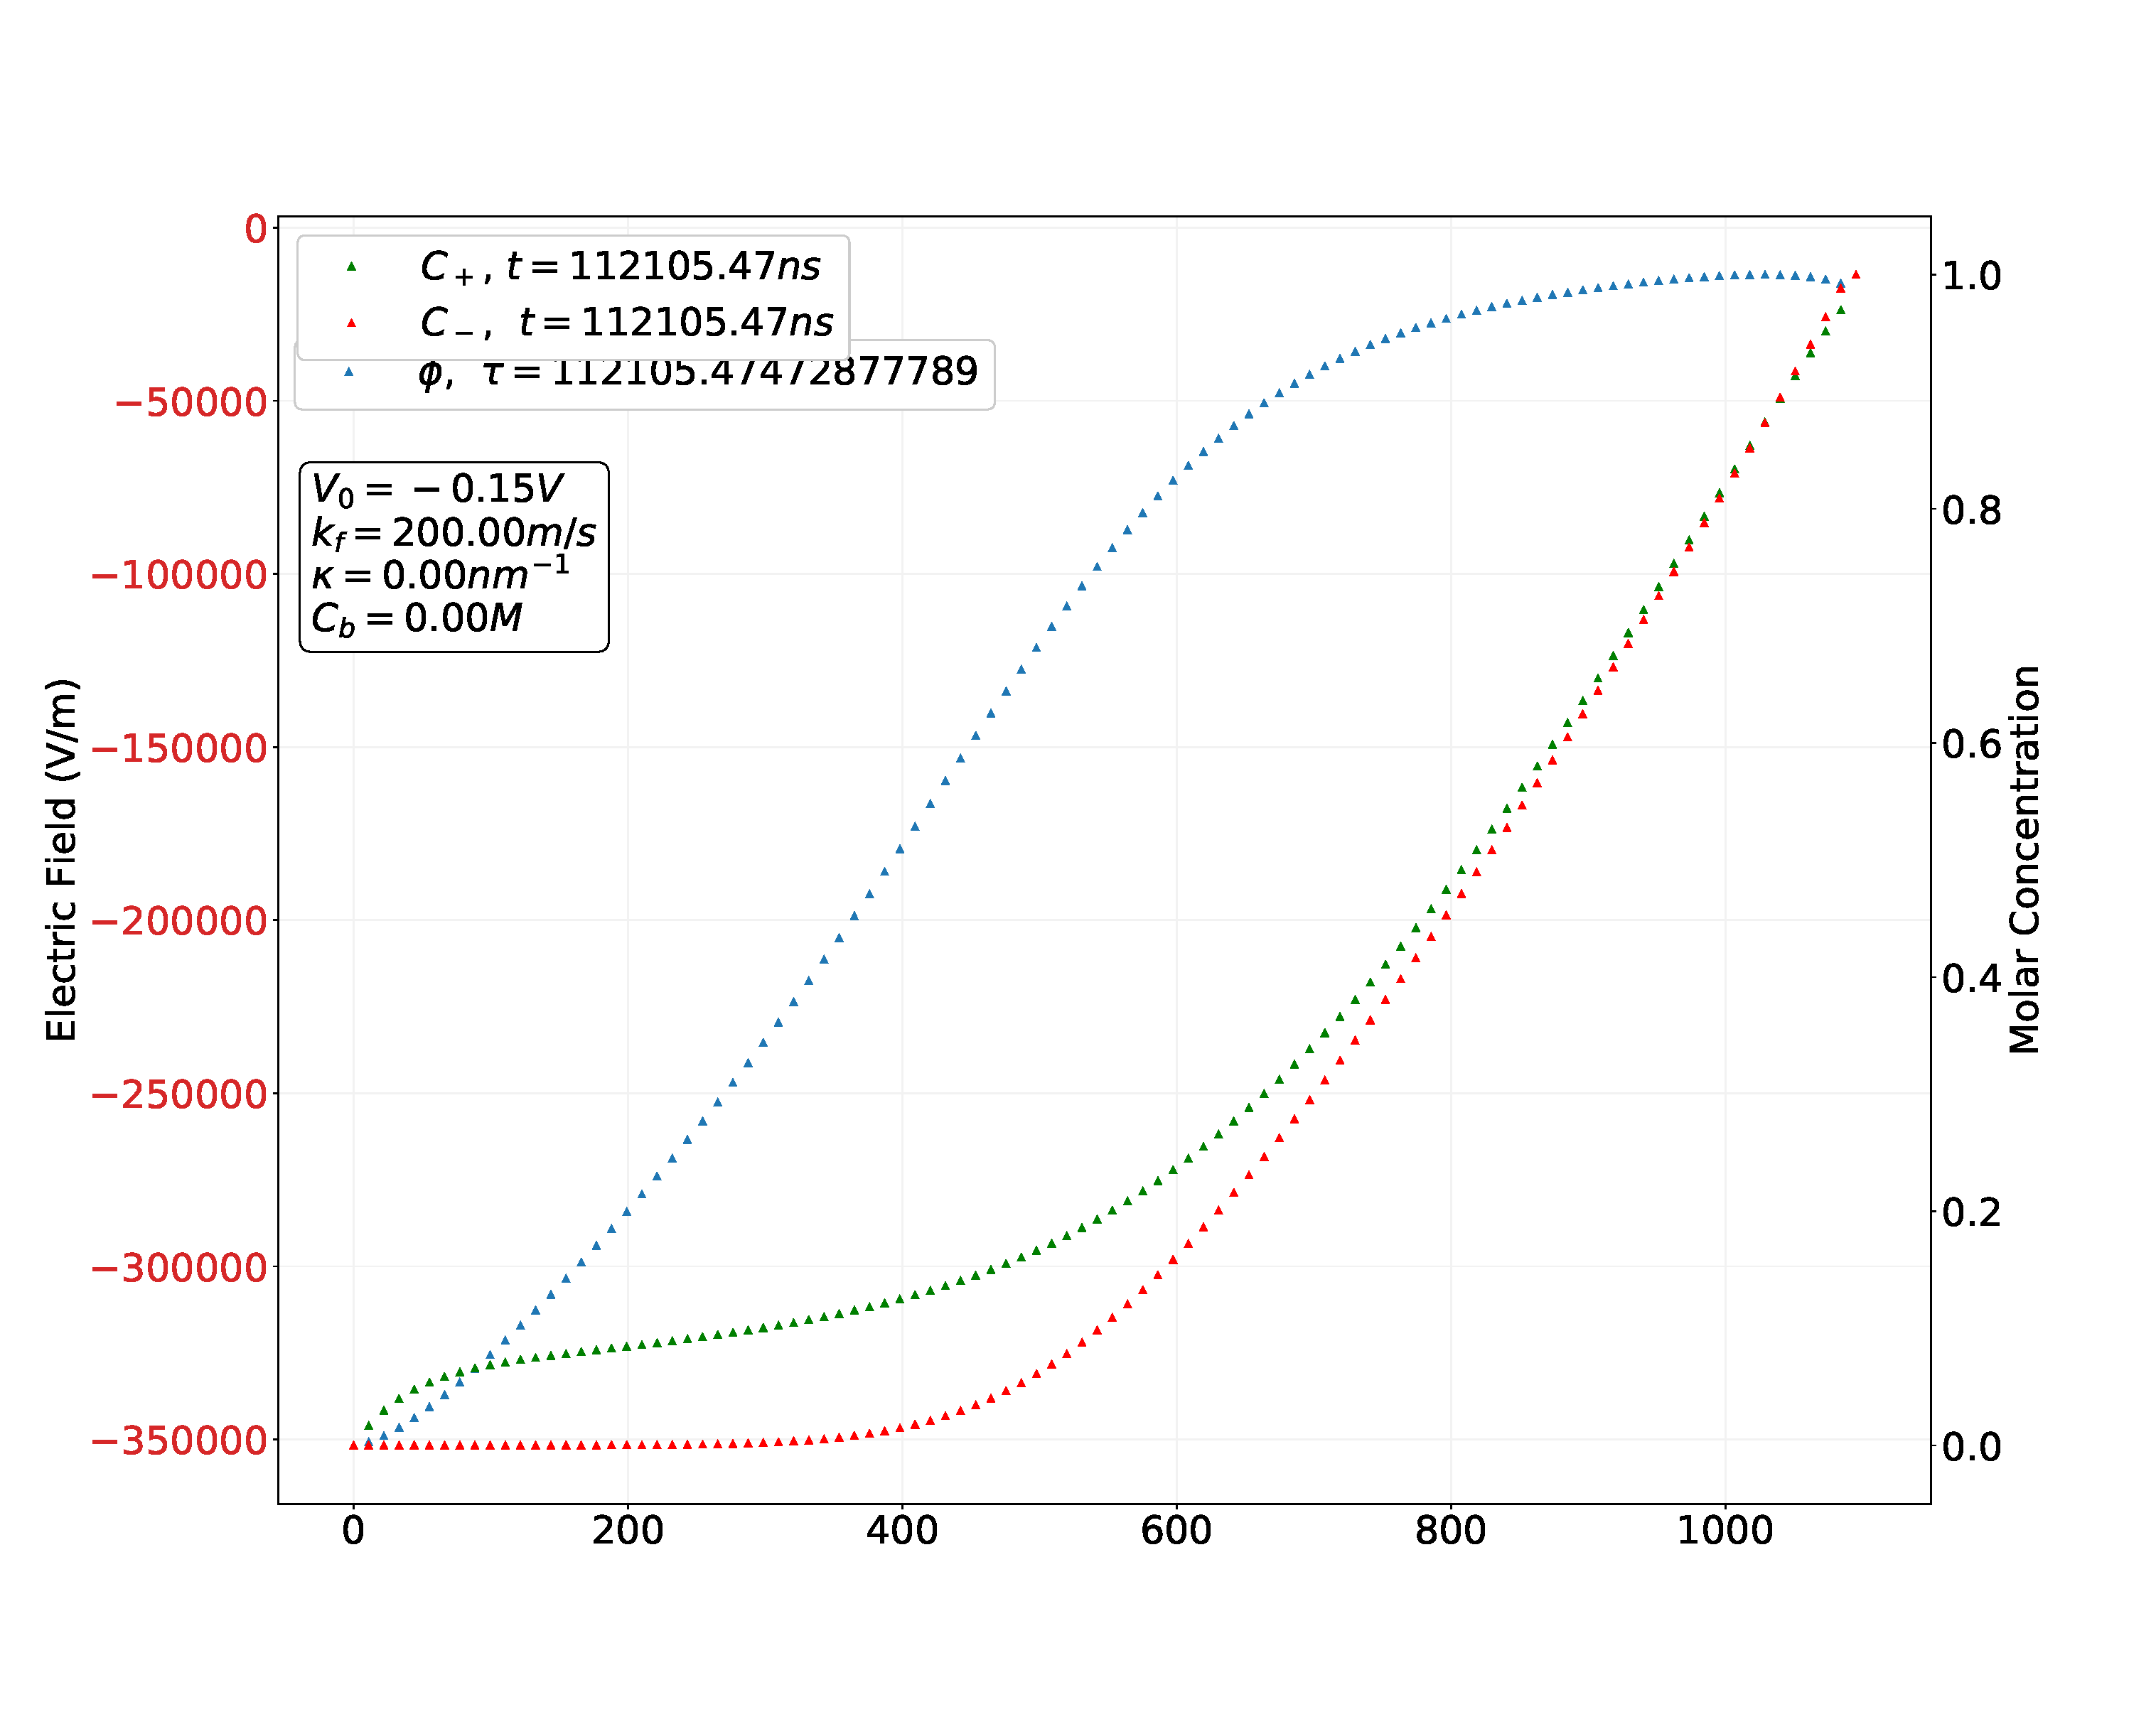
\includegraphics[width =\textwidth]{complete-diffusion-nernstE1.eps}
\caption{}
\label{fig:ef2}
\end{subfigure}\\[1ex]
\begin{subfigure}{\linewidth}
\centering
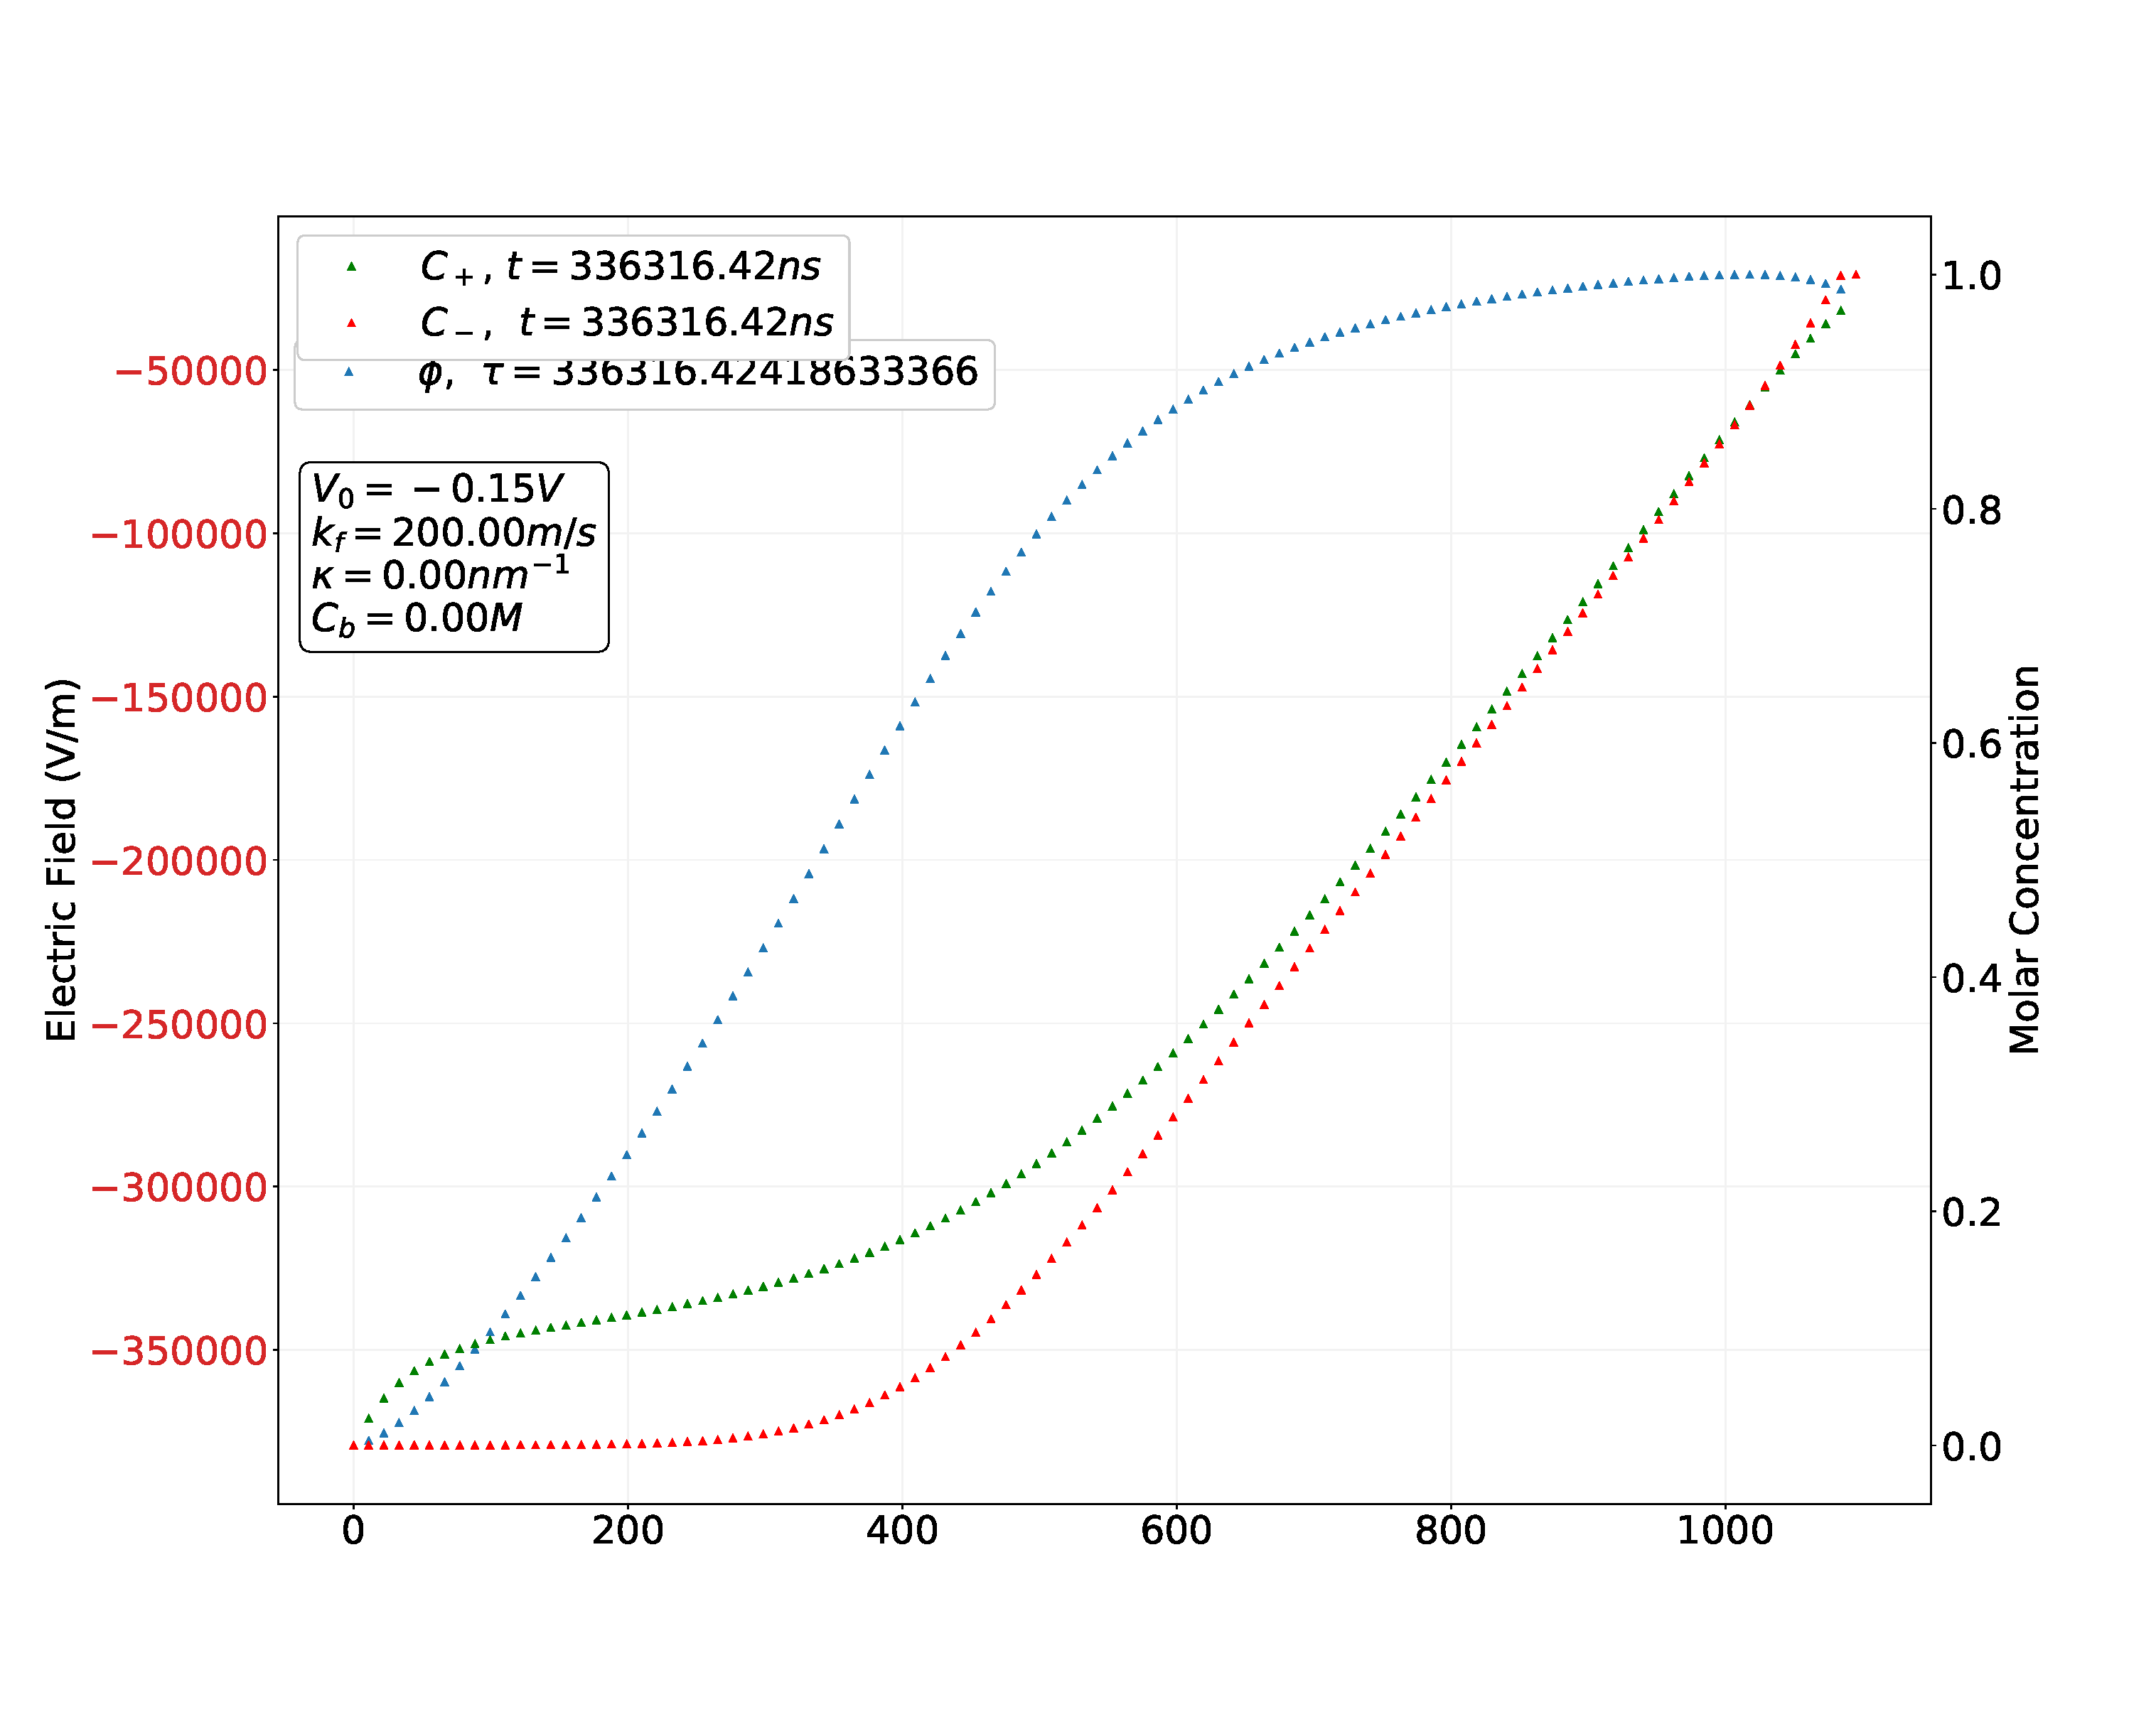
\includegraphics[width =0.5\textwidth]{complete-diffusion-nernstE2.eps}
\caption{}
\label{fig:ef3}
\end{subfigure}
\caption{Electric field and concentration of $Cu^{+2}$ (green dots) and $SO_4^{-2}$ (blue dots) at (a) $t = 0.448 ns$, (b) $t = 2.24 ns$ and (c) $t = 4.44 ns$}.
\label{fig:test}
\end{figure}

\begin{figure}[htbp]
\centering
\textbf{Electric Potential In The Diffusion Problem With Nernst Interaction.}\par\medskip
\begin{subfigure}{.5\linewidth}
\centering
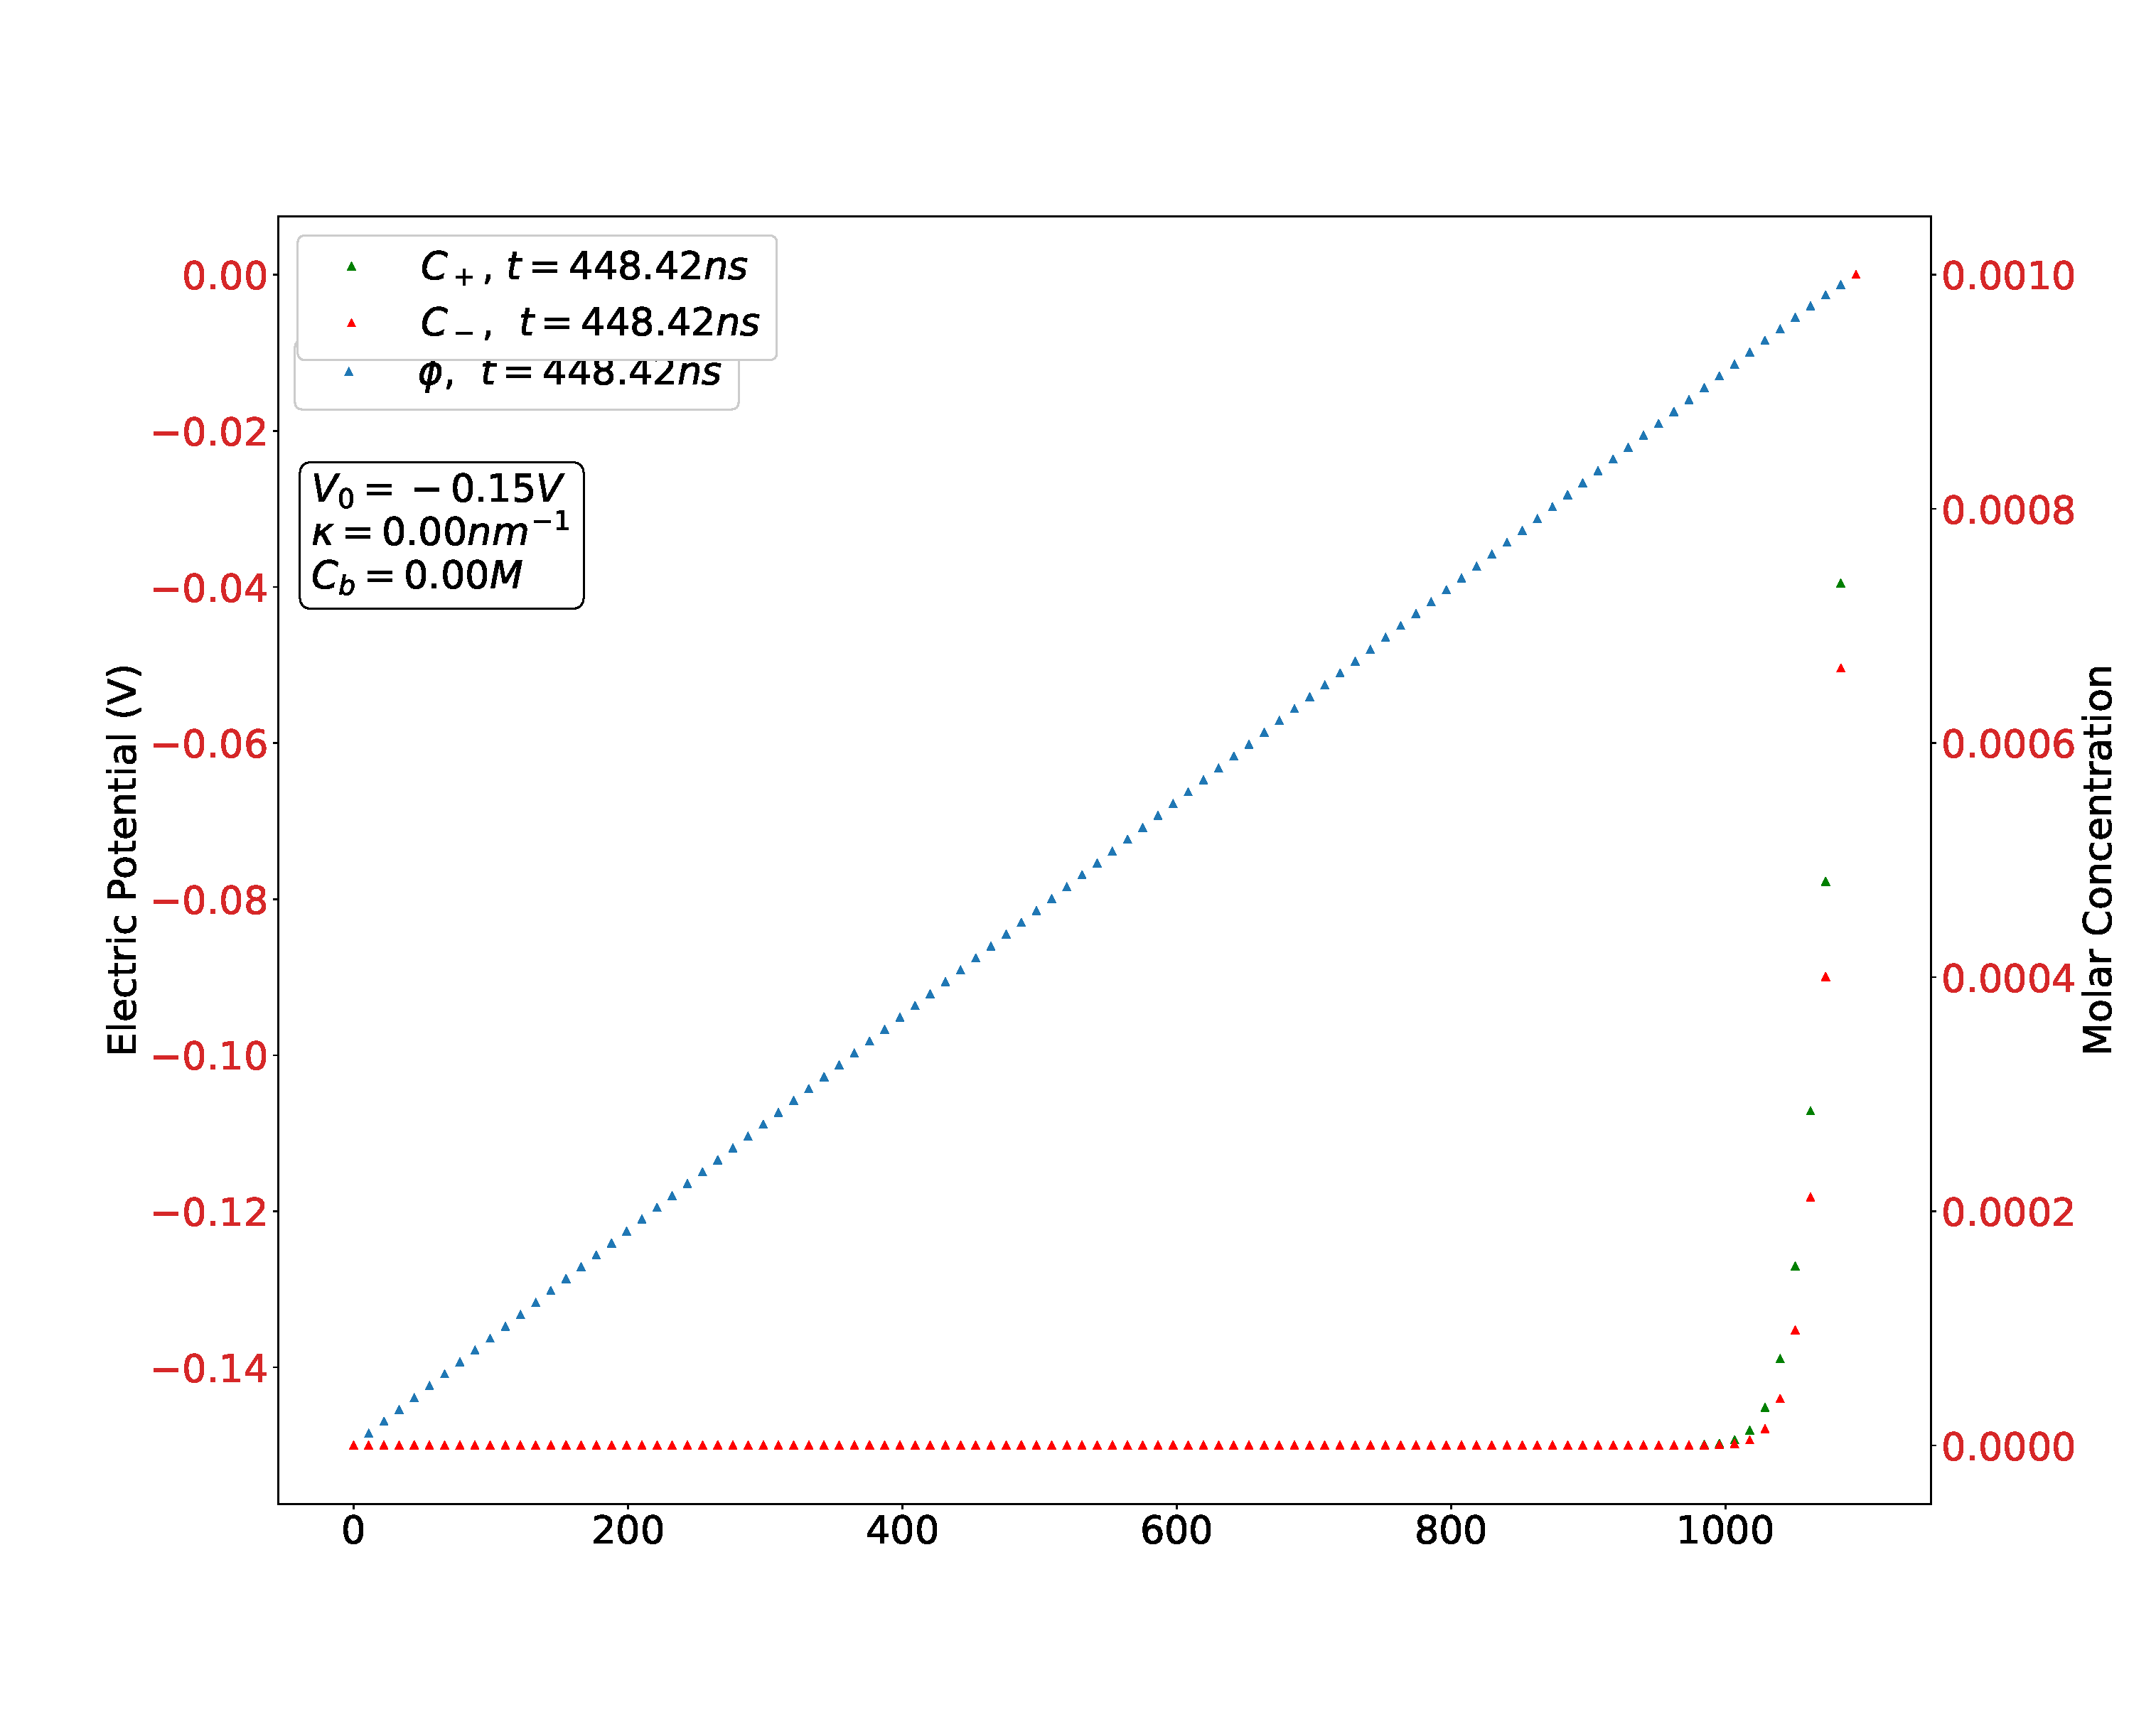
\includegraphics[width=\textwidth]{complete-diffusion-nernstphi0.eps}
\caption{}
\label{fig:ef1}
\end{subfigure}%
\begin{subfigure}{.5\linewidth}
\centering
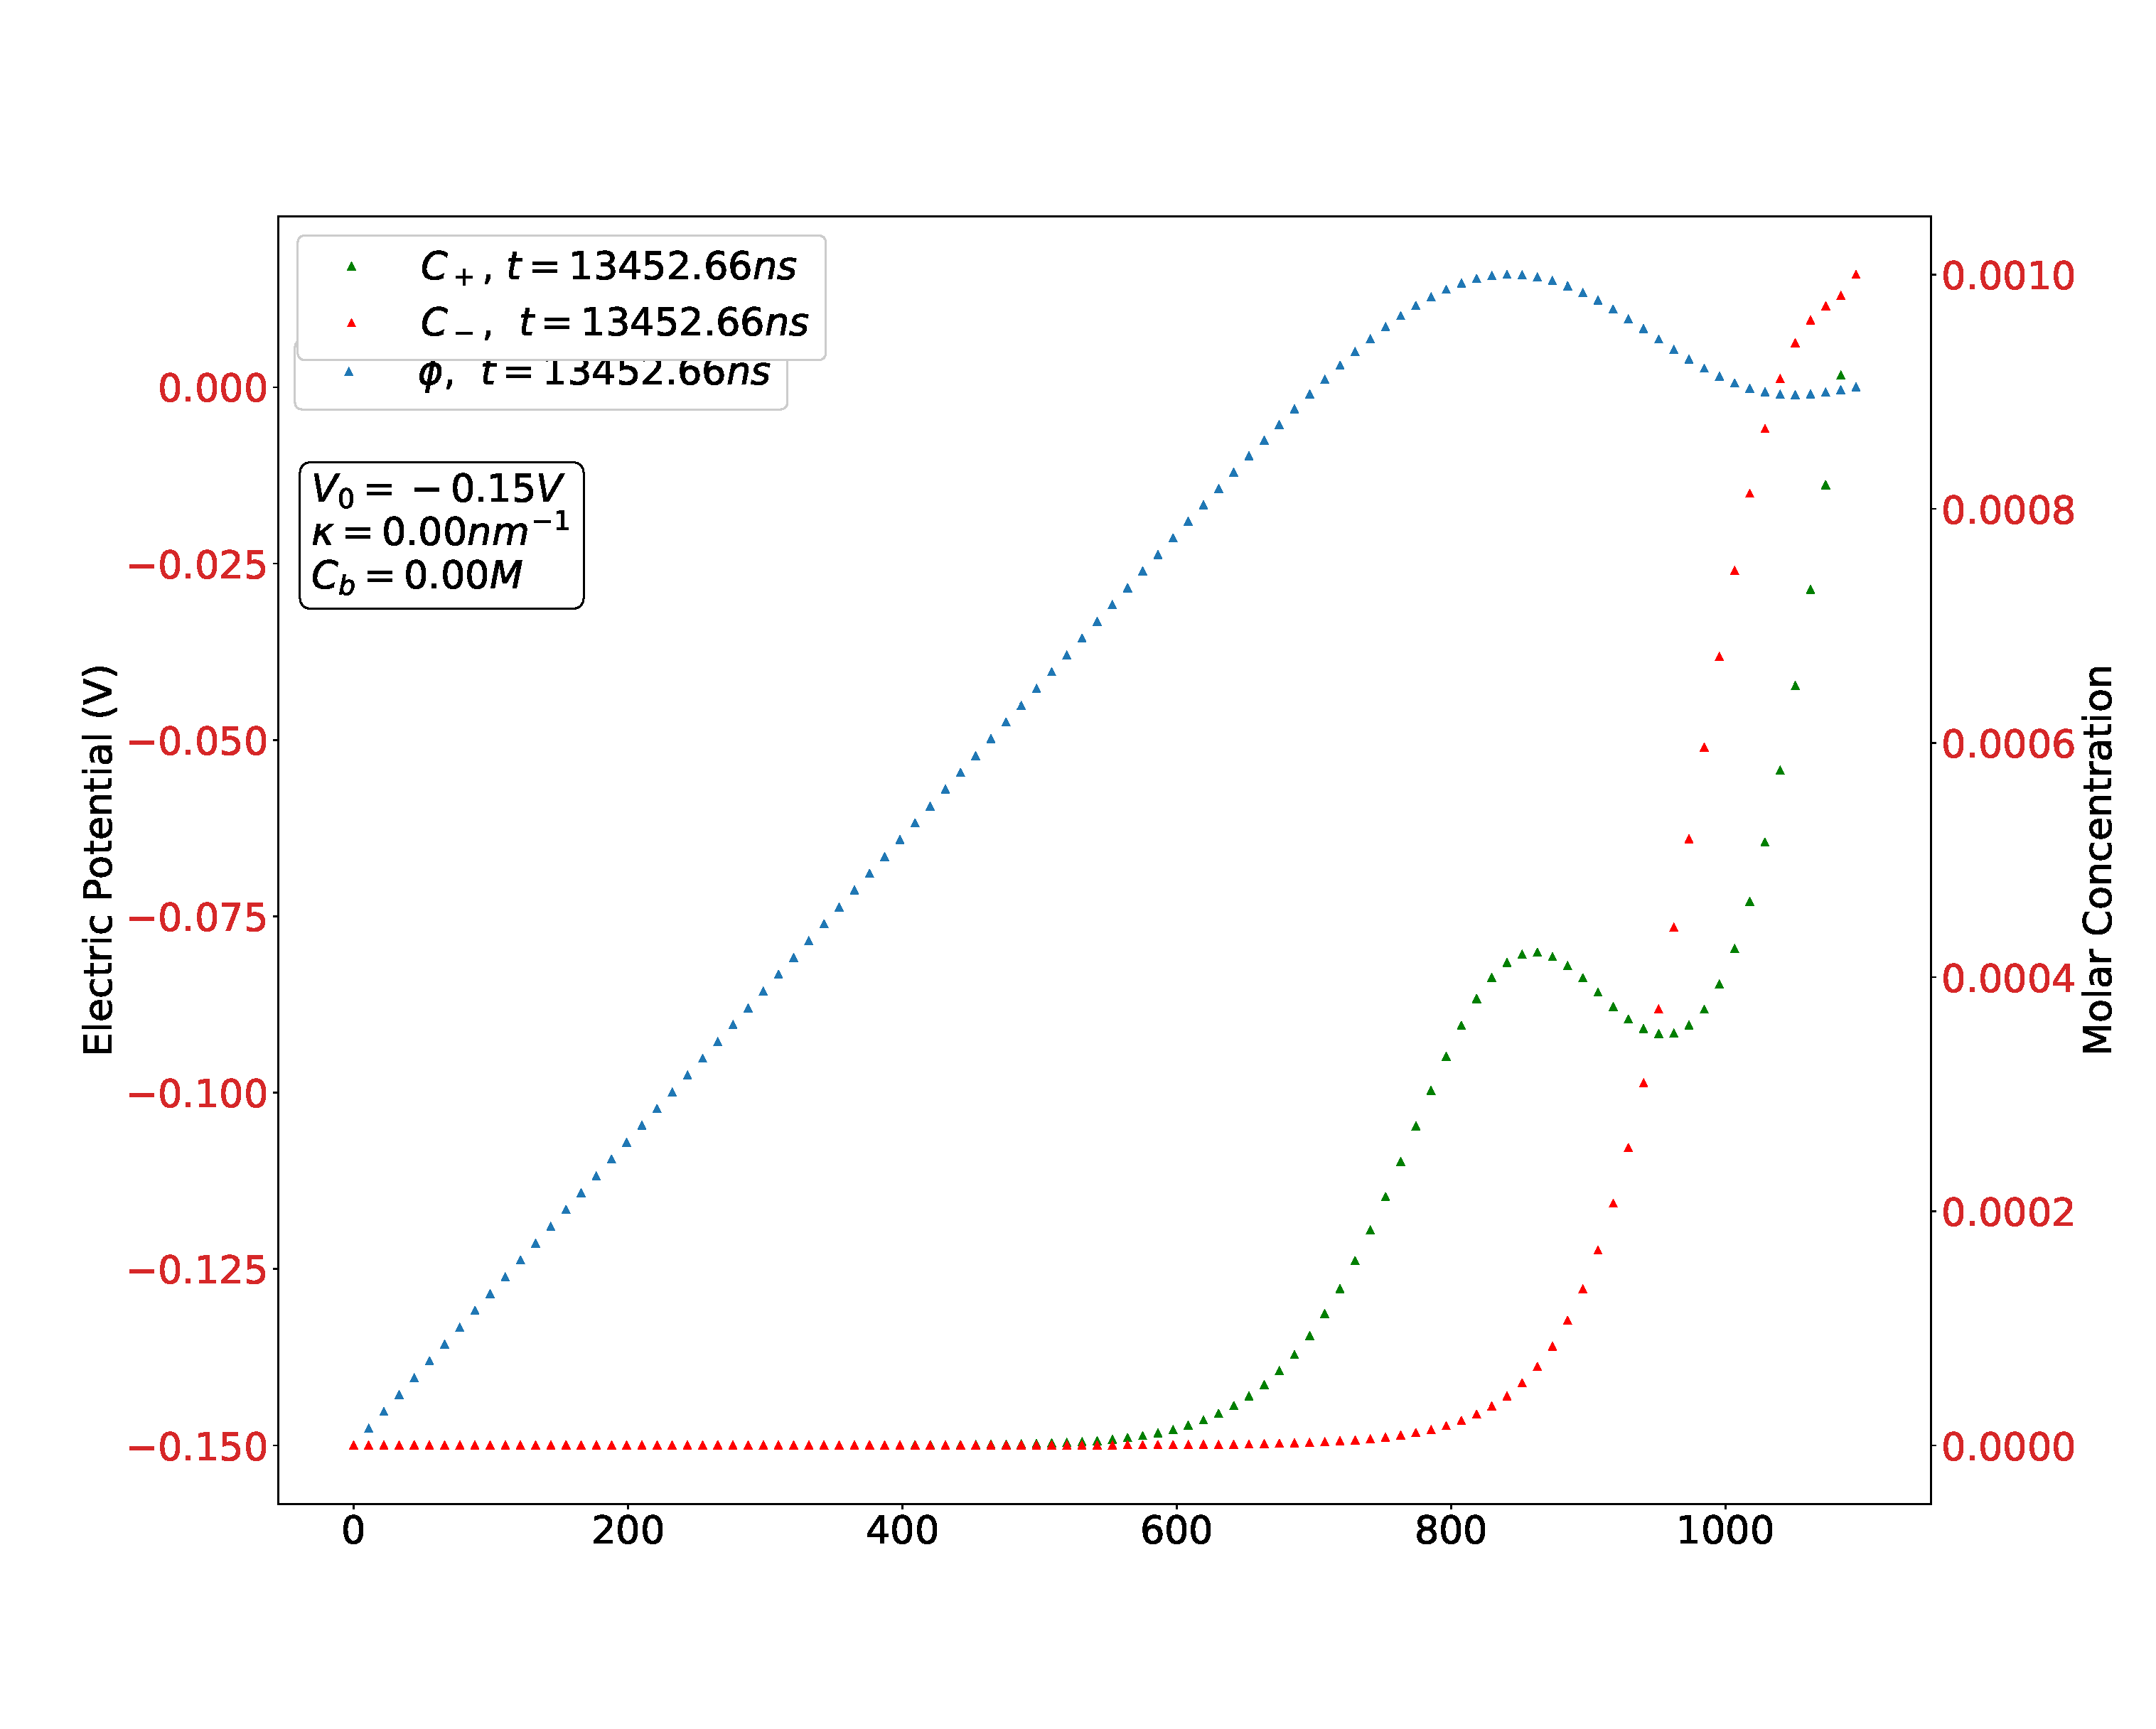
\includegraphics[width =\textwidth]{complete-diffusion-nernstphi1.eps}
\caption{}
\label{fig:ef2}
\end{subfigure}\\[1ex]
\begin{subfigure}{\linewidth}
\centering
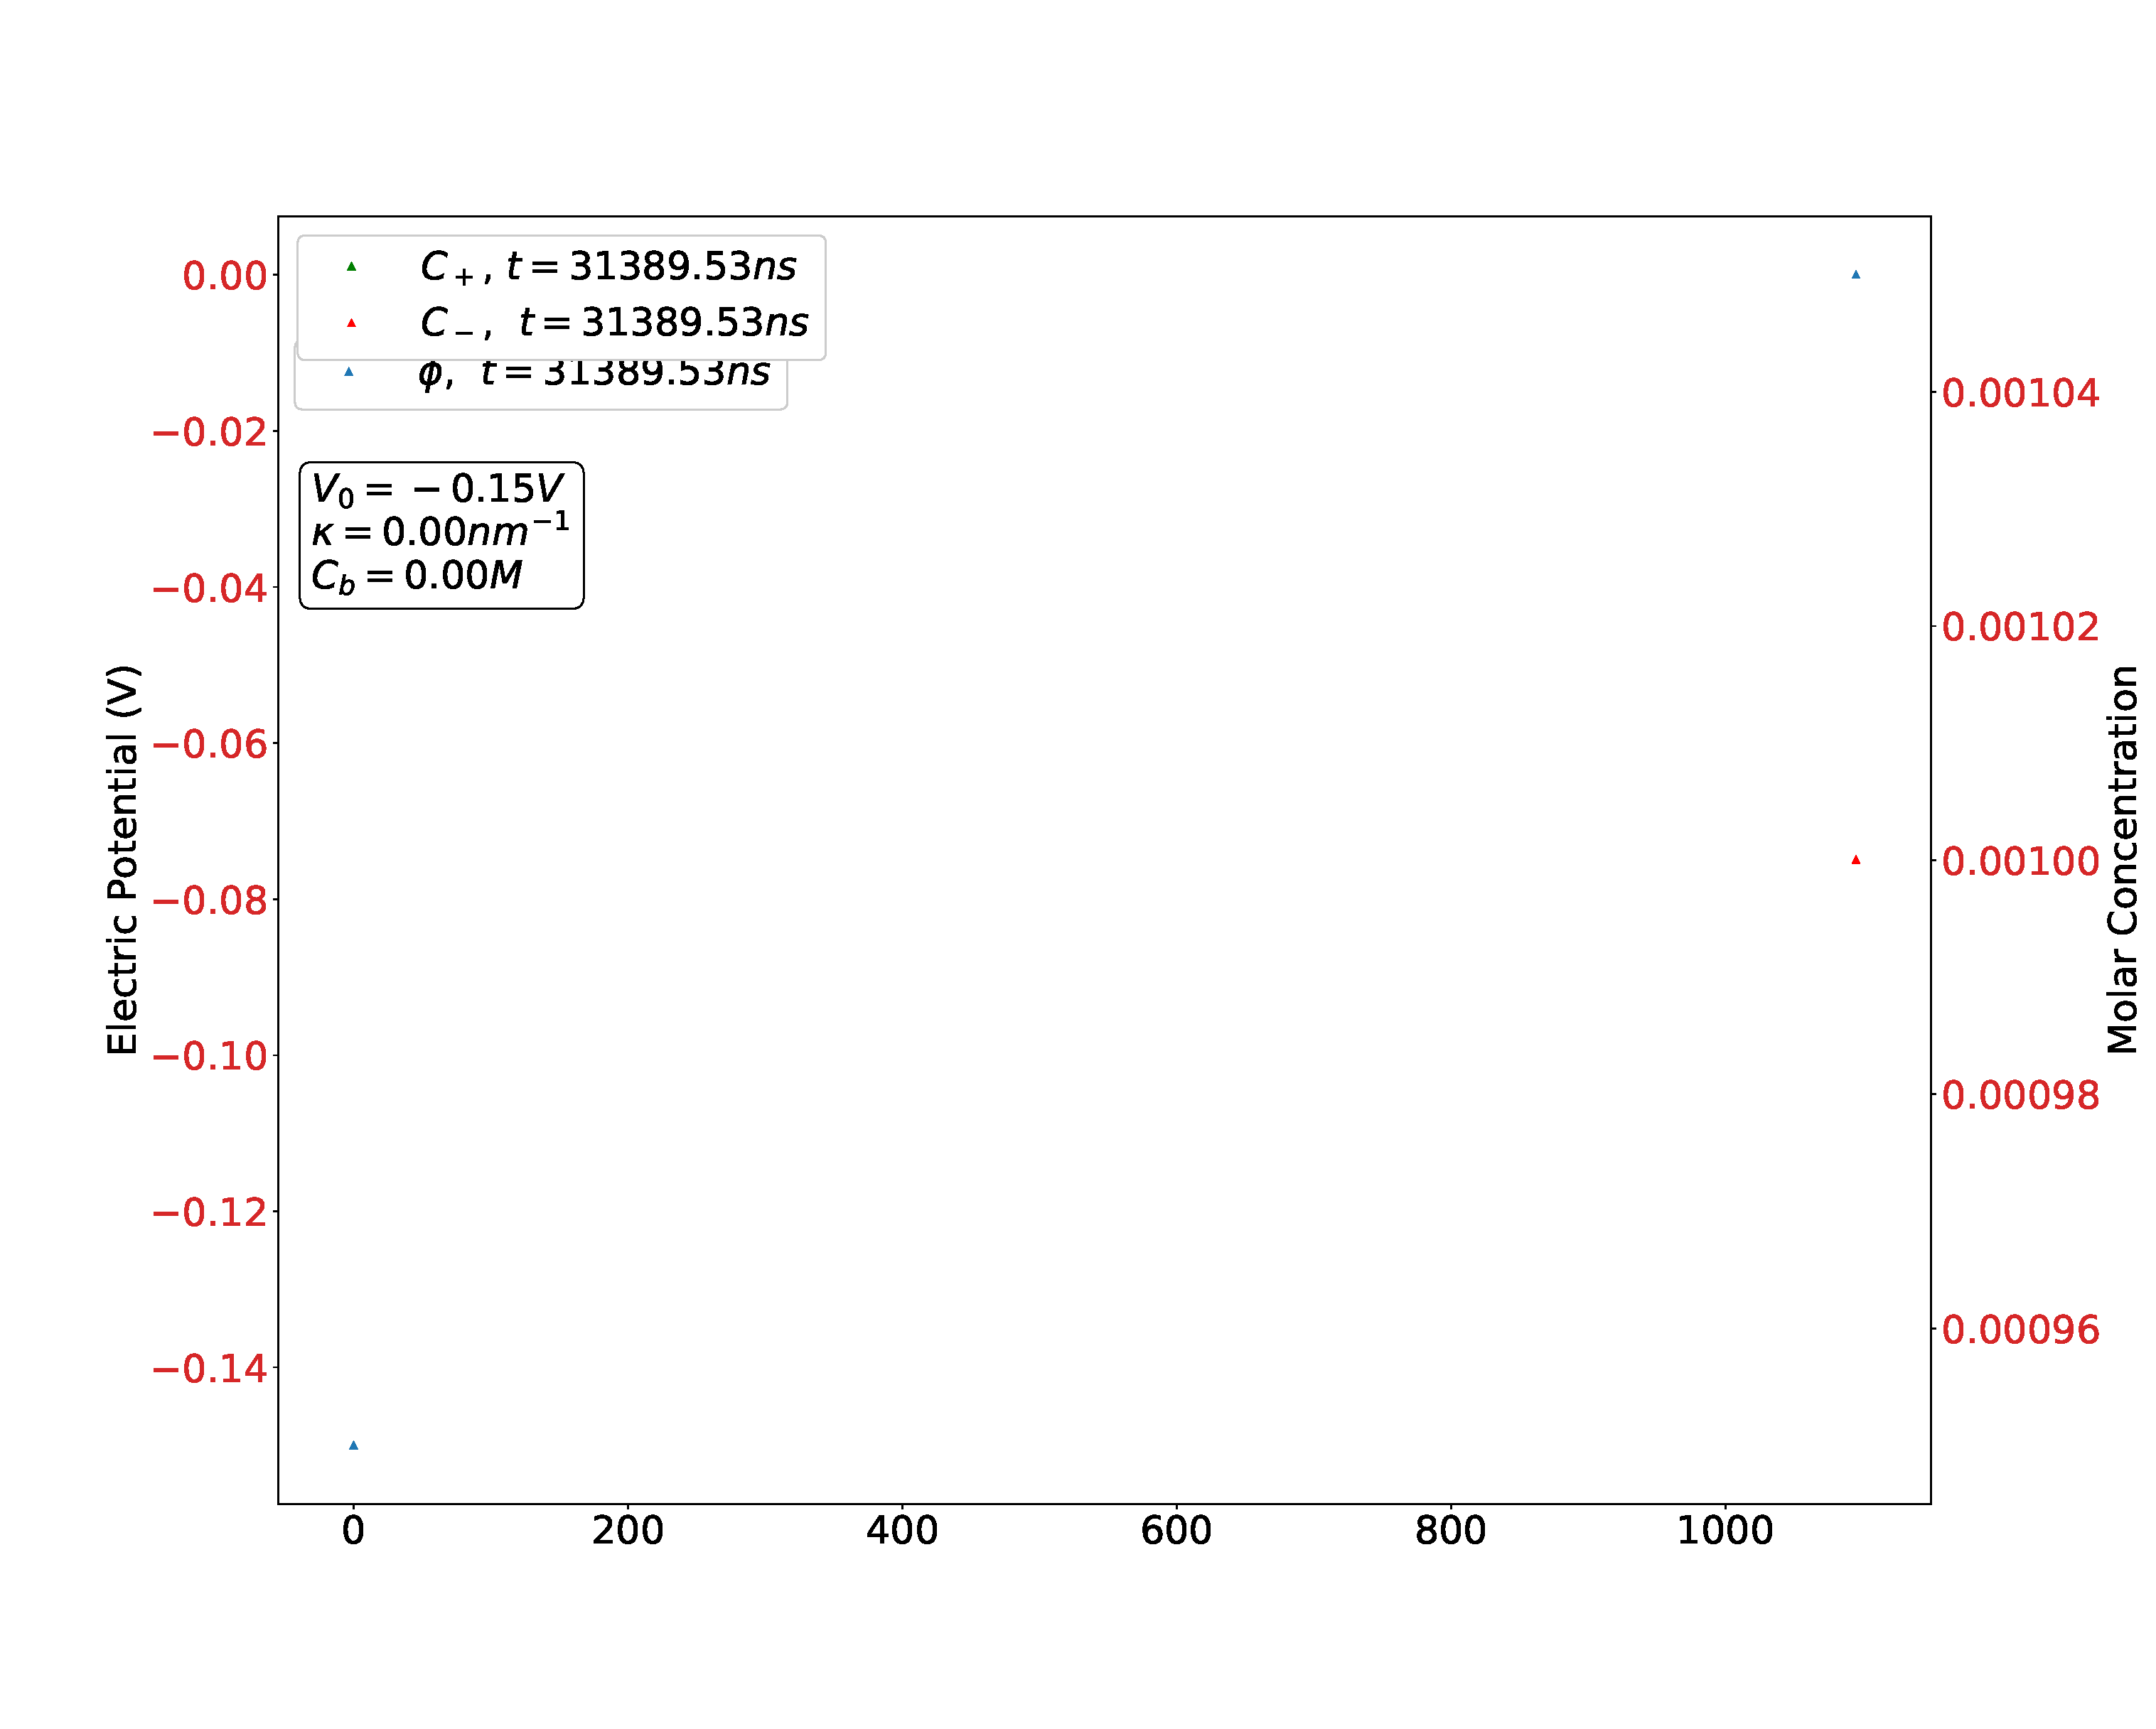
\includegraphics[width =0.5\textwidth]{complete-diffusion-nernstphi2.eps}
\caption{}
\label{fig:ef3}
\end{subfigure}
\caption{Electric potential in volts and molar concentration of $Cu^{+2}$ (green dots) and $SO_4^{-2}$ (blue dots) at (a) $t = 0.448 ns$, (b) $t = 2.24 ns$ and (c) $t = 4.44 ns$}
\label{fig:test}
\end{figure}


\newpage
\subsection{Electric field at the surface of the electrode}

A feature of interest is the electric field at the surface. As measurements by a solid state device would be done by implanting the device on the surface, we are interested in how would the electric field vary as the model's parameters fluctuate. Particularly, we are interested in how the electric field varies with voltage and with the bulk concentration.

\begin{figure}[htbp]
\centering
\textbf{Electric field at the surface.}\par\medskip
\begin{subfigure}{.5\linewidth}
\centering
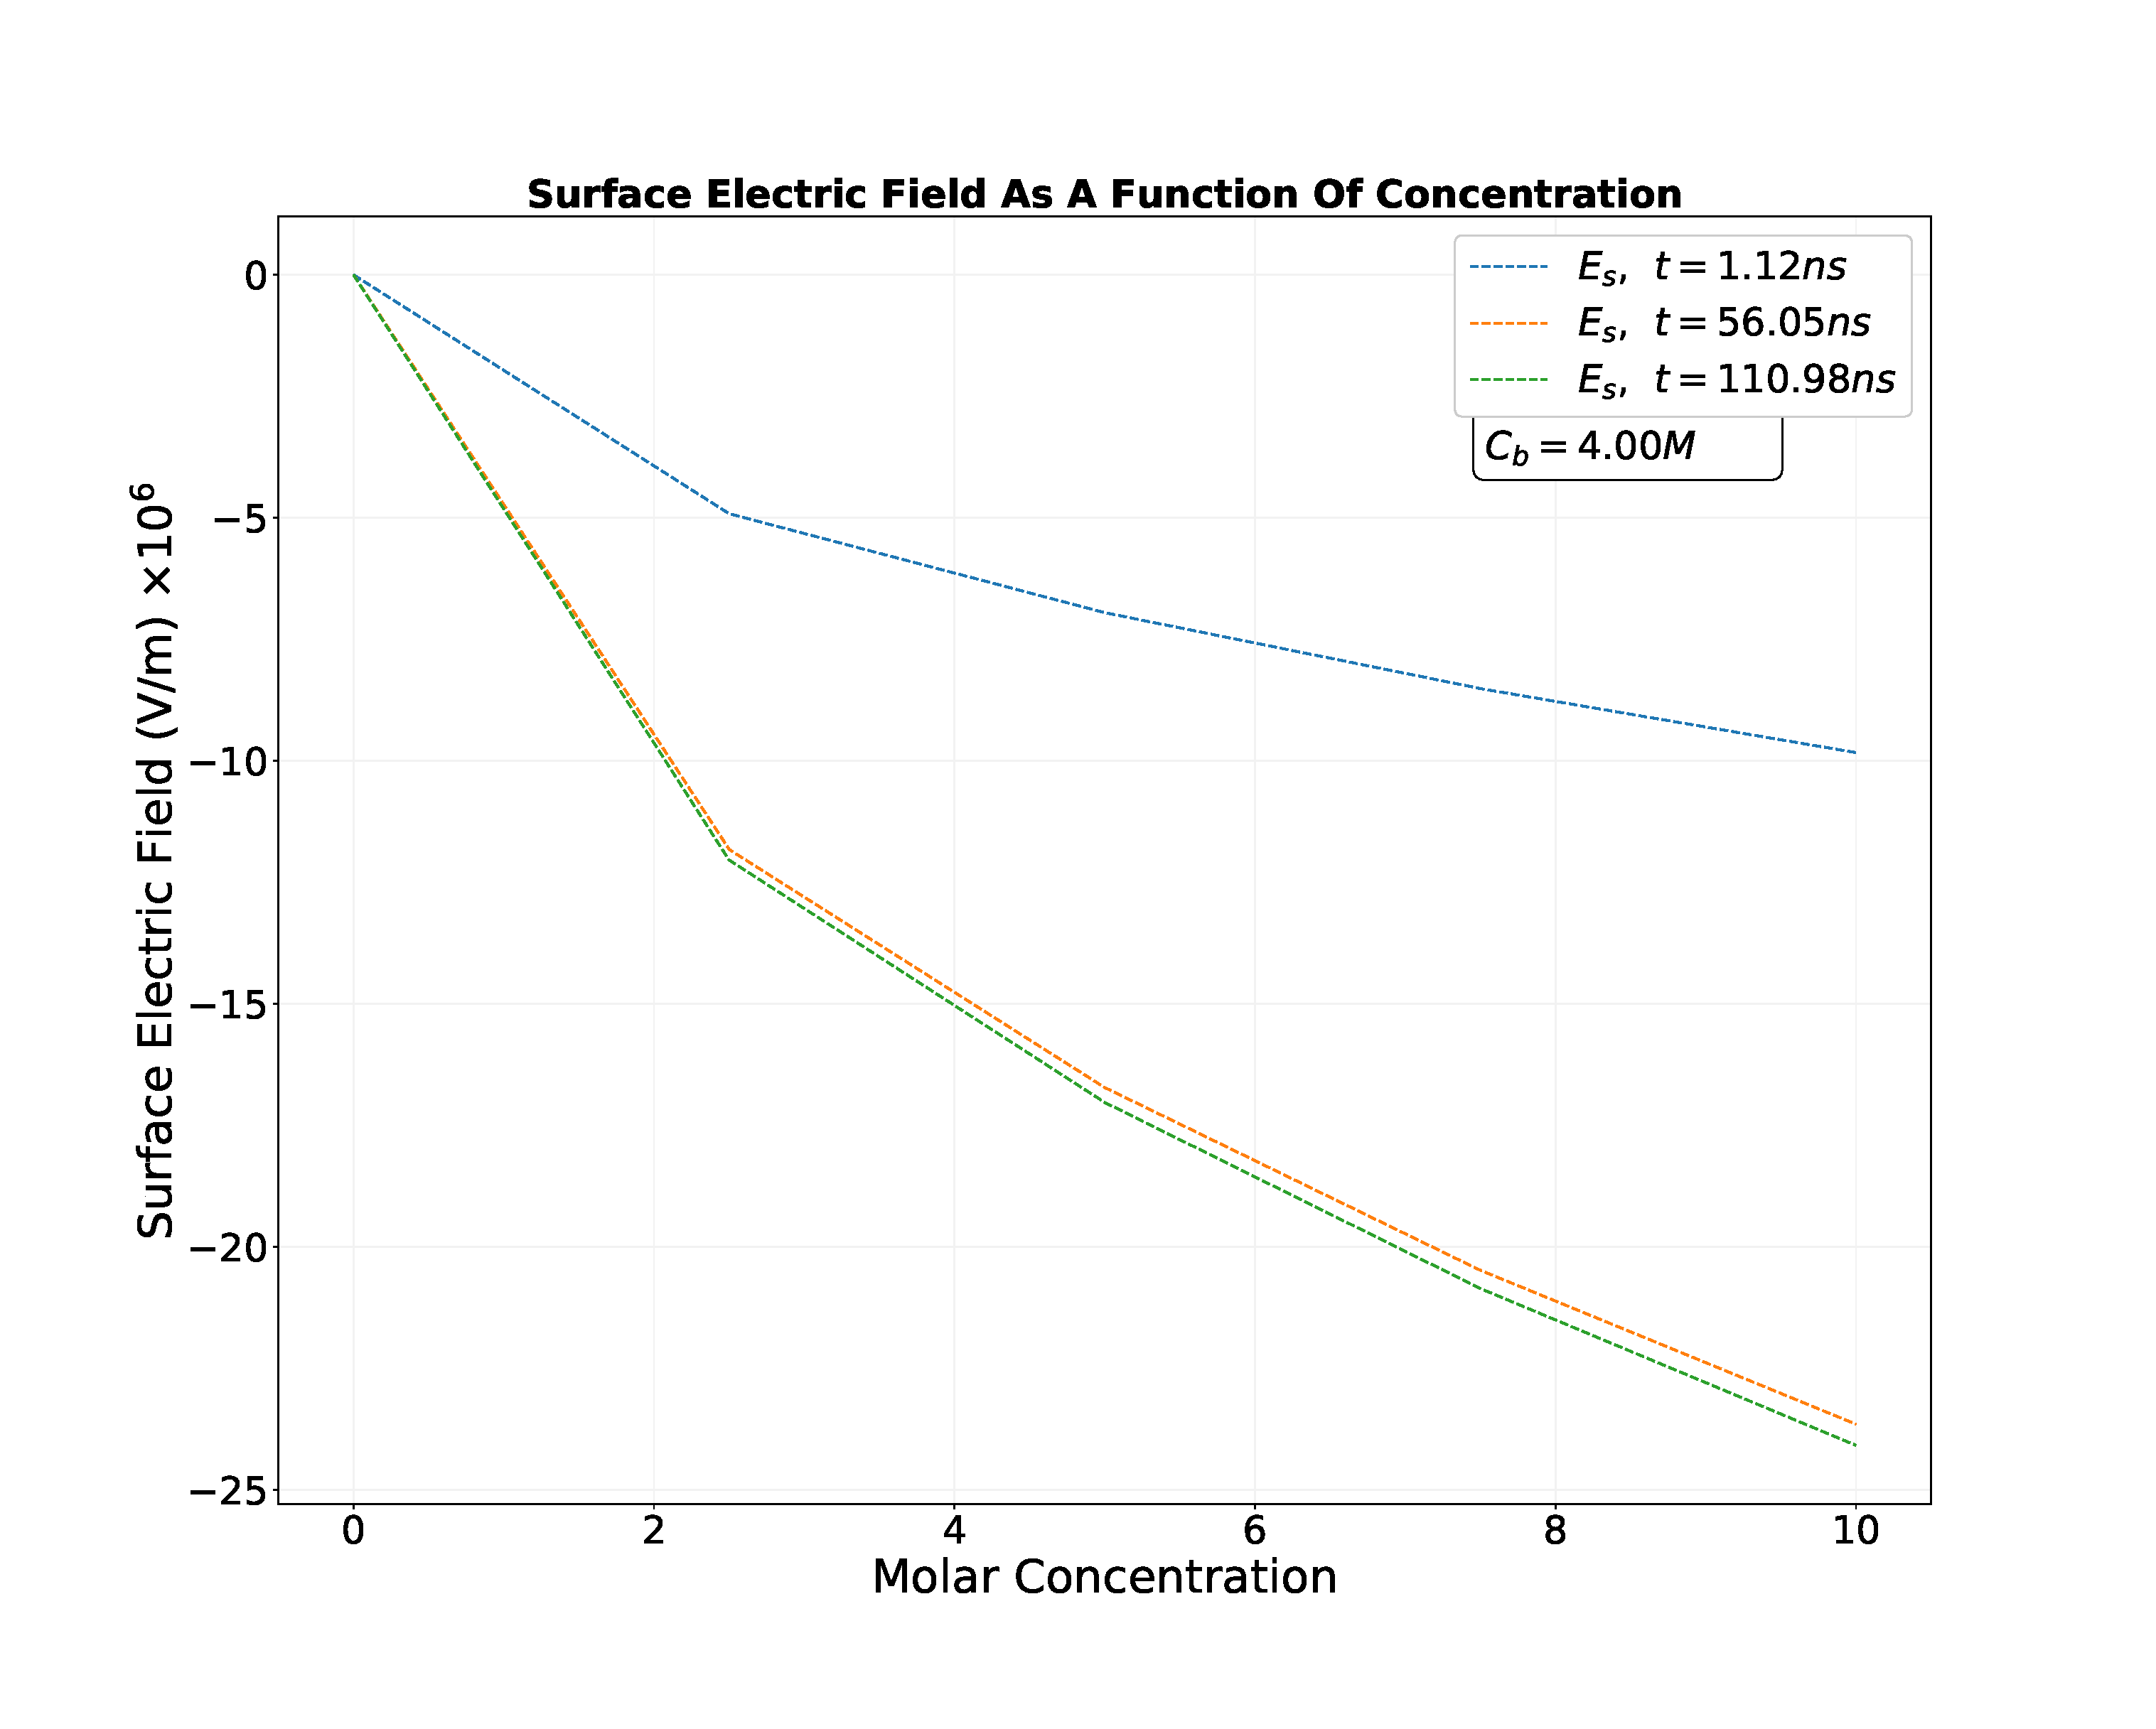
\includegraphics[width=\textwidth]{surfaceEfield_Cb.eps}
\caption{}
\label{fig:ef1}
\end{subfigure}%
\begin{subfigure}{.5\linewidth}
\centering
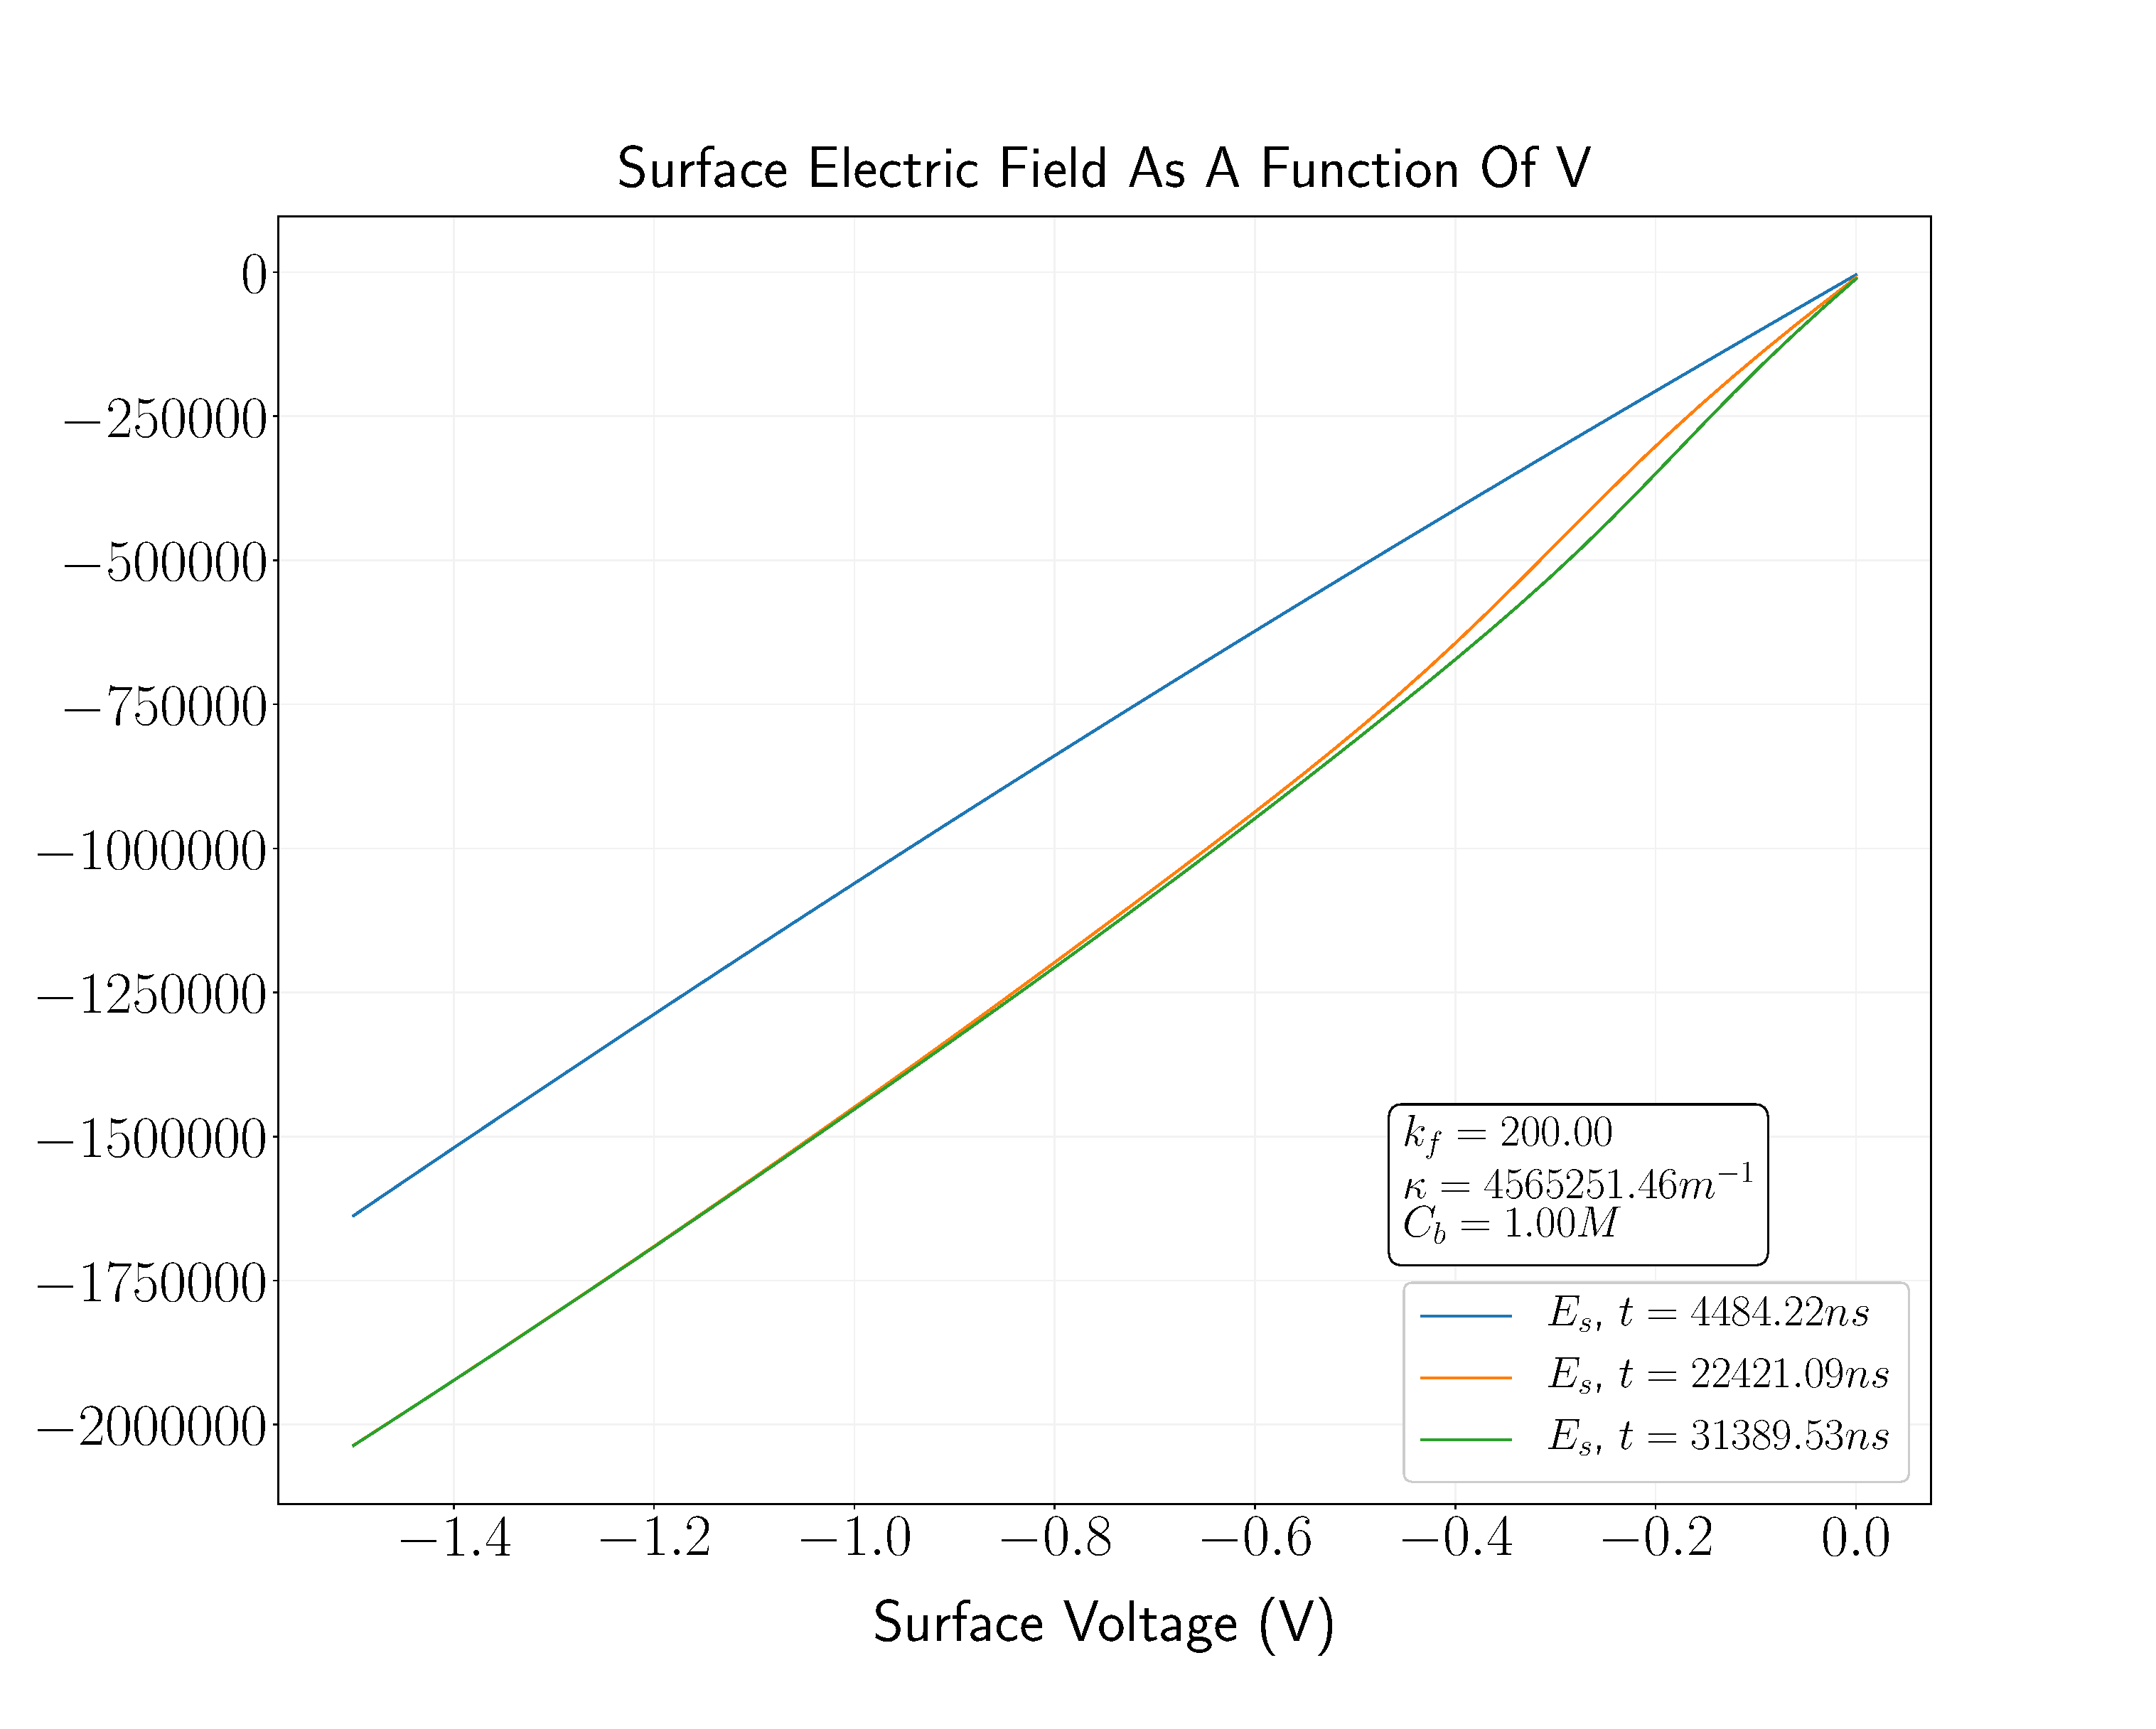
\includegraphics[width =\textwidth]{surfaceEfield_v.eps}
\caption{}
\label{fig:ef2}
\end{subfigure}\\[1ex]
\caption{(a) Electric field at the surface as a function of the molar concentration of the original salt. Dependence occurs through the model parameter $\kappa$ called the ionic force \ref{eq:ionic-force} (b) Electric field at the surface $x=0$ of the electrode as a function of the voltage at the plate, which is a boundary condition to the Poisson equation \ref{eq:system}}
\label{fig:test}
\end{figure}




\newpage
\subsection{Grounded electrode limit}

In the case of $V_0 = \Psi_0 = 0$ we get a purely diffusive process, as expected. Figure can compare figure \ref{fig:analytic-results} to figure \ref{fig:nernts-no-field}


\begin{figure}[htbp]
\centering
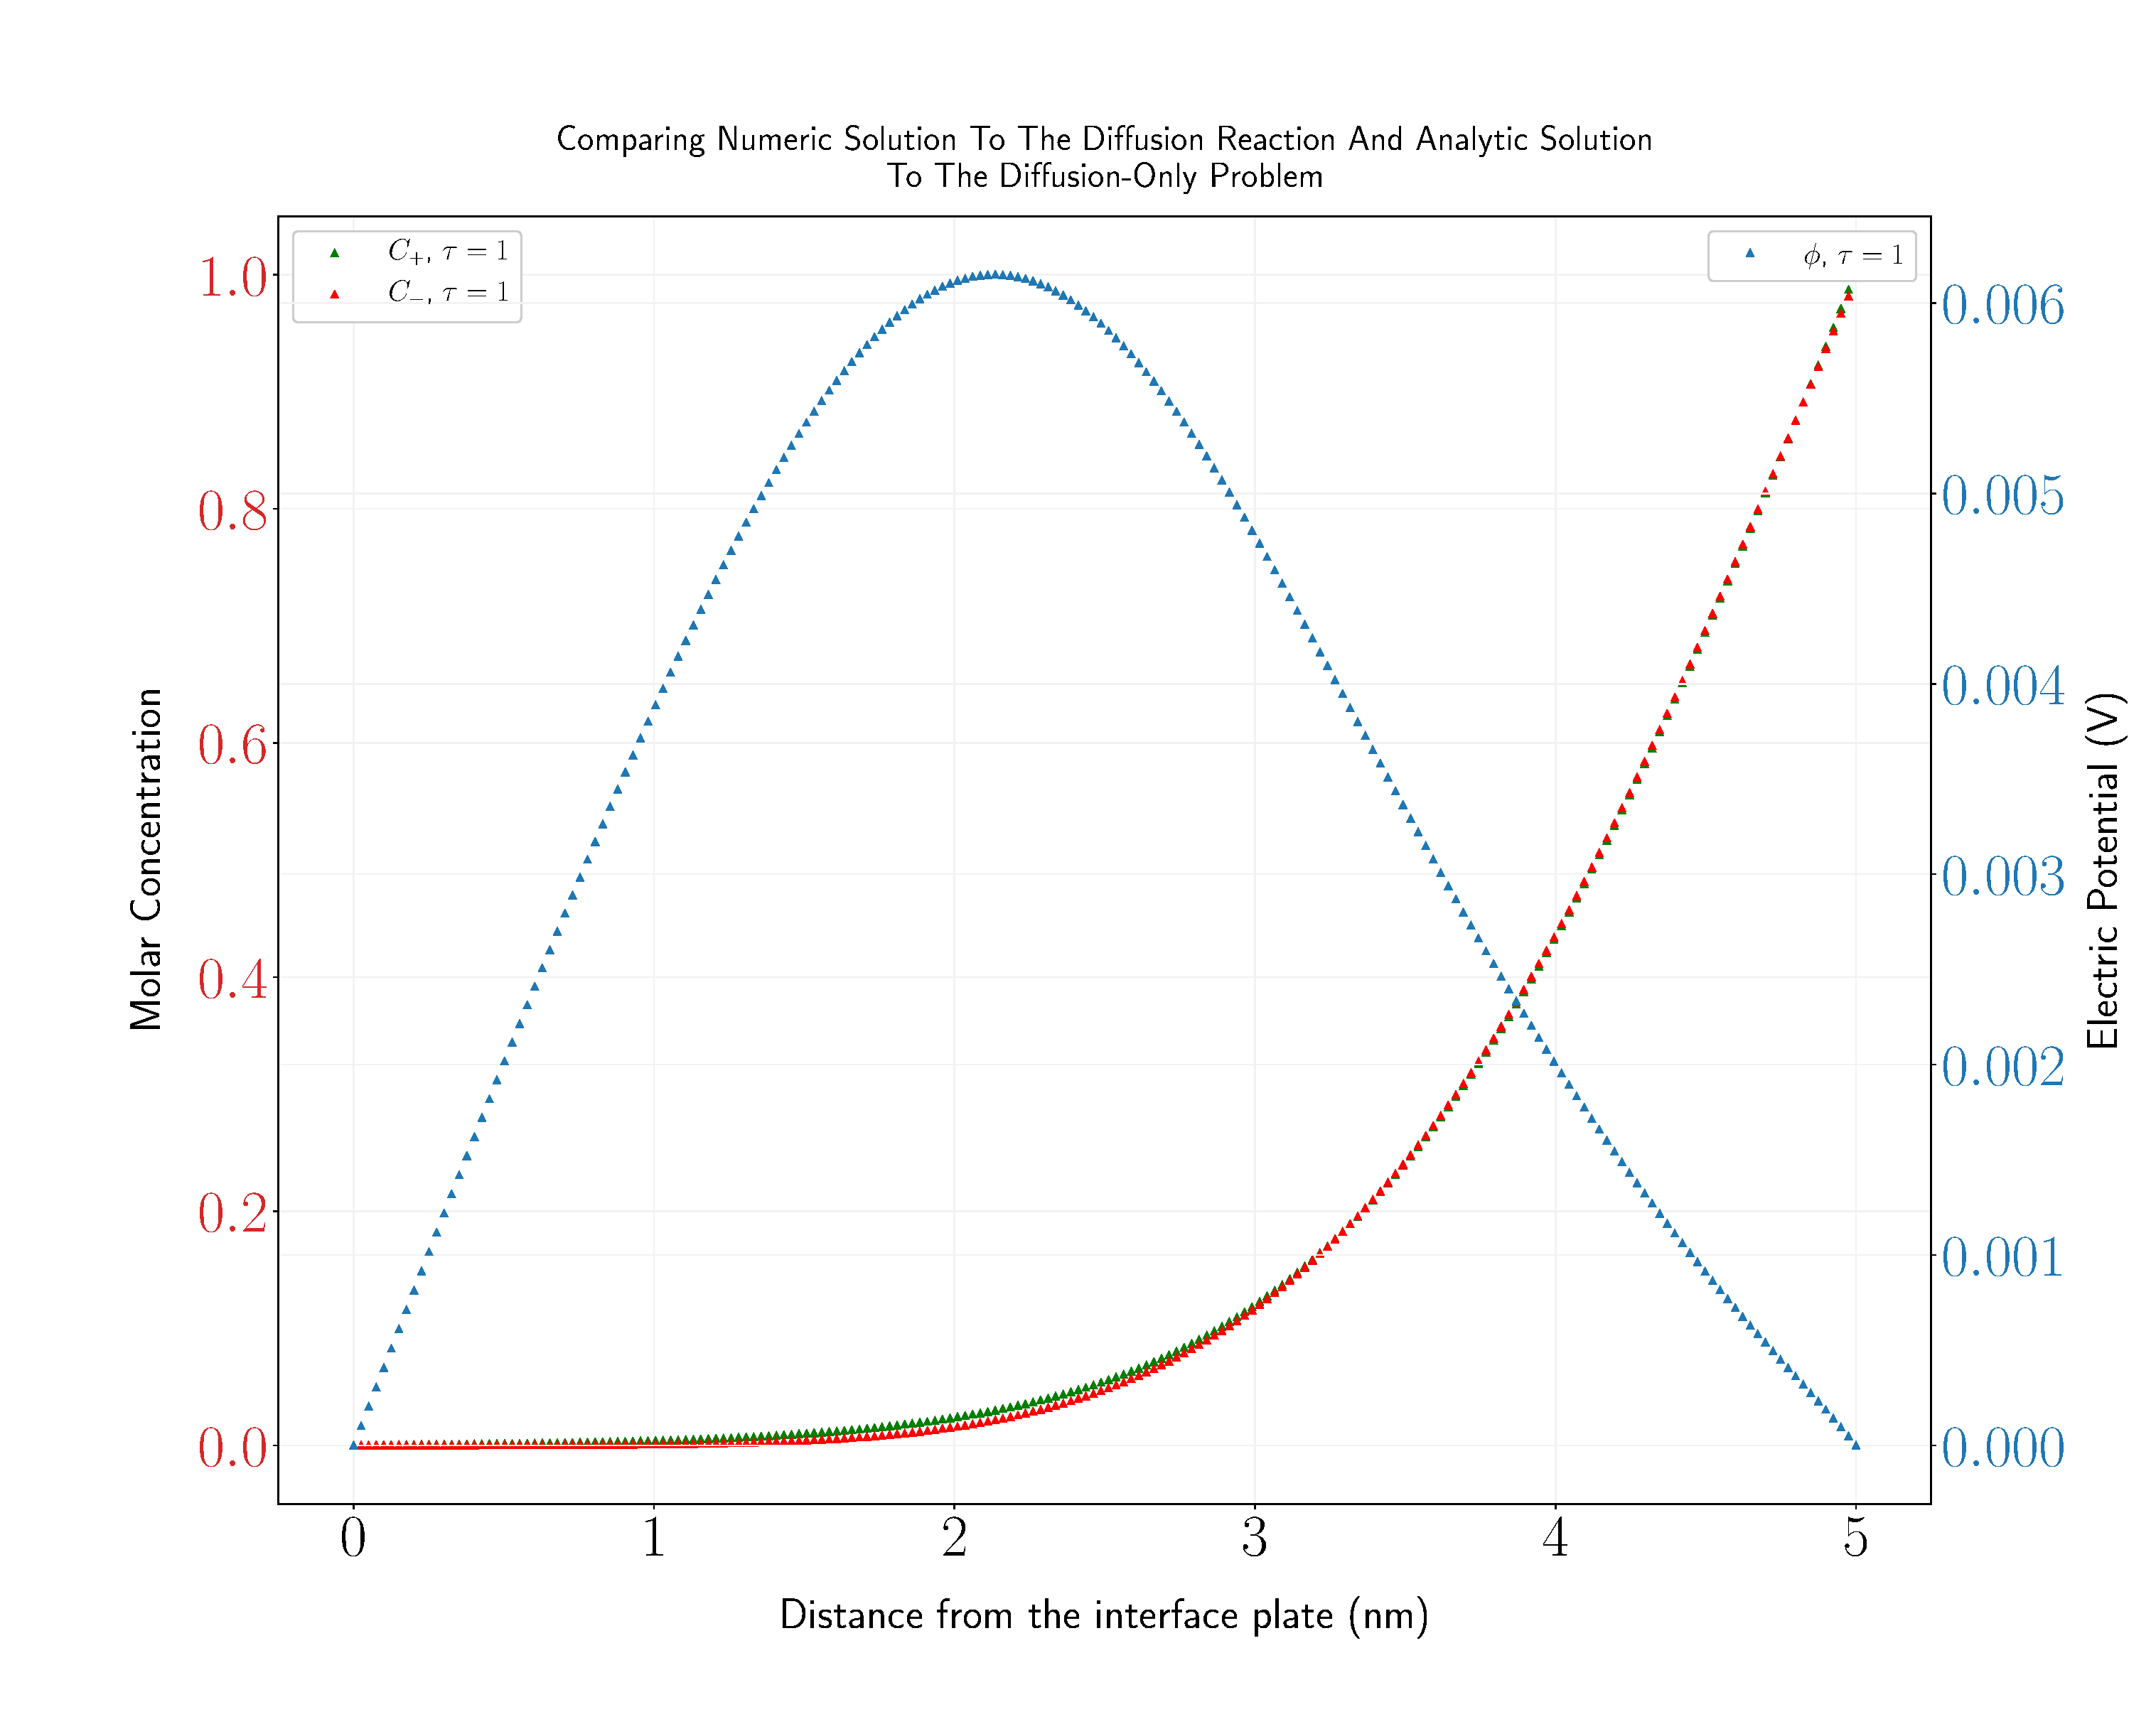
\includegraphics[width=\textwidth]{complete-no-electric-field.eps}
\caption{In the no-electrode limit we take $V_0=0$ in order to see the behavior diffusive-only limit. The electric field is zero throughout the system as an initial condition. The blue dots show the electric field due te the screening of the electrolyte in solution. }
\label{fig:nernts-no-field}
\end{figure}


\newpage
\subsection{Electric Field Fluctuation As A Function Of Time}


A quantity of great interest is the fluctuation of the electric field with respect to the steady state solution. Particularly, we are interested in studying such fluctuations at the interface with the electrode. Such fluctuations are defined as

\begin{align}
	\delta E(t) = E(x=0, t) - E_{SS}(x=0), 
\end{align}

where 

\begin{align}
	E_{SS}(x) = \lim_{t\rightarrow\infty} E(x,t).
\end{align}



\begin{figure}[htbp]
\centering
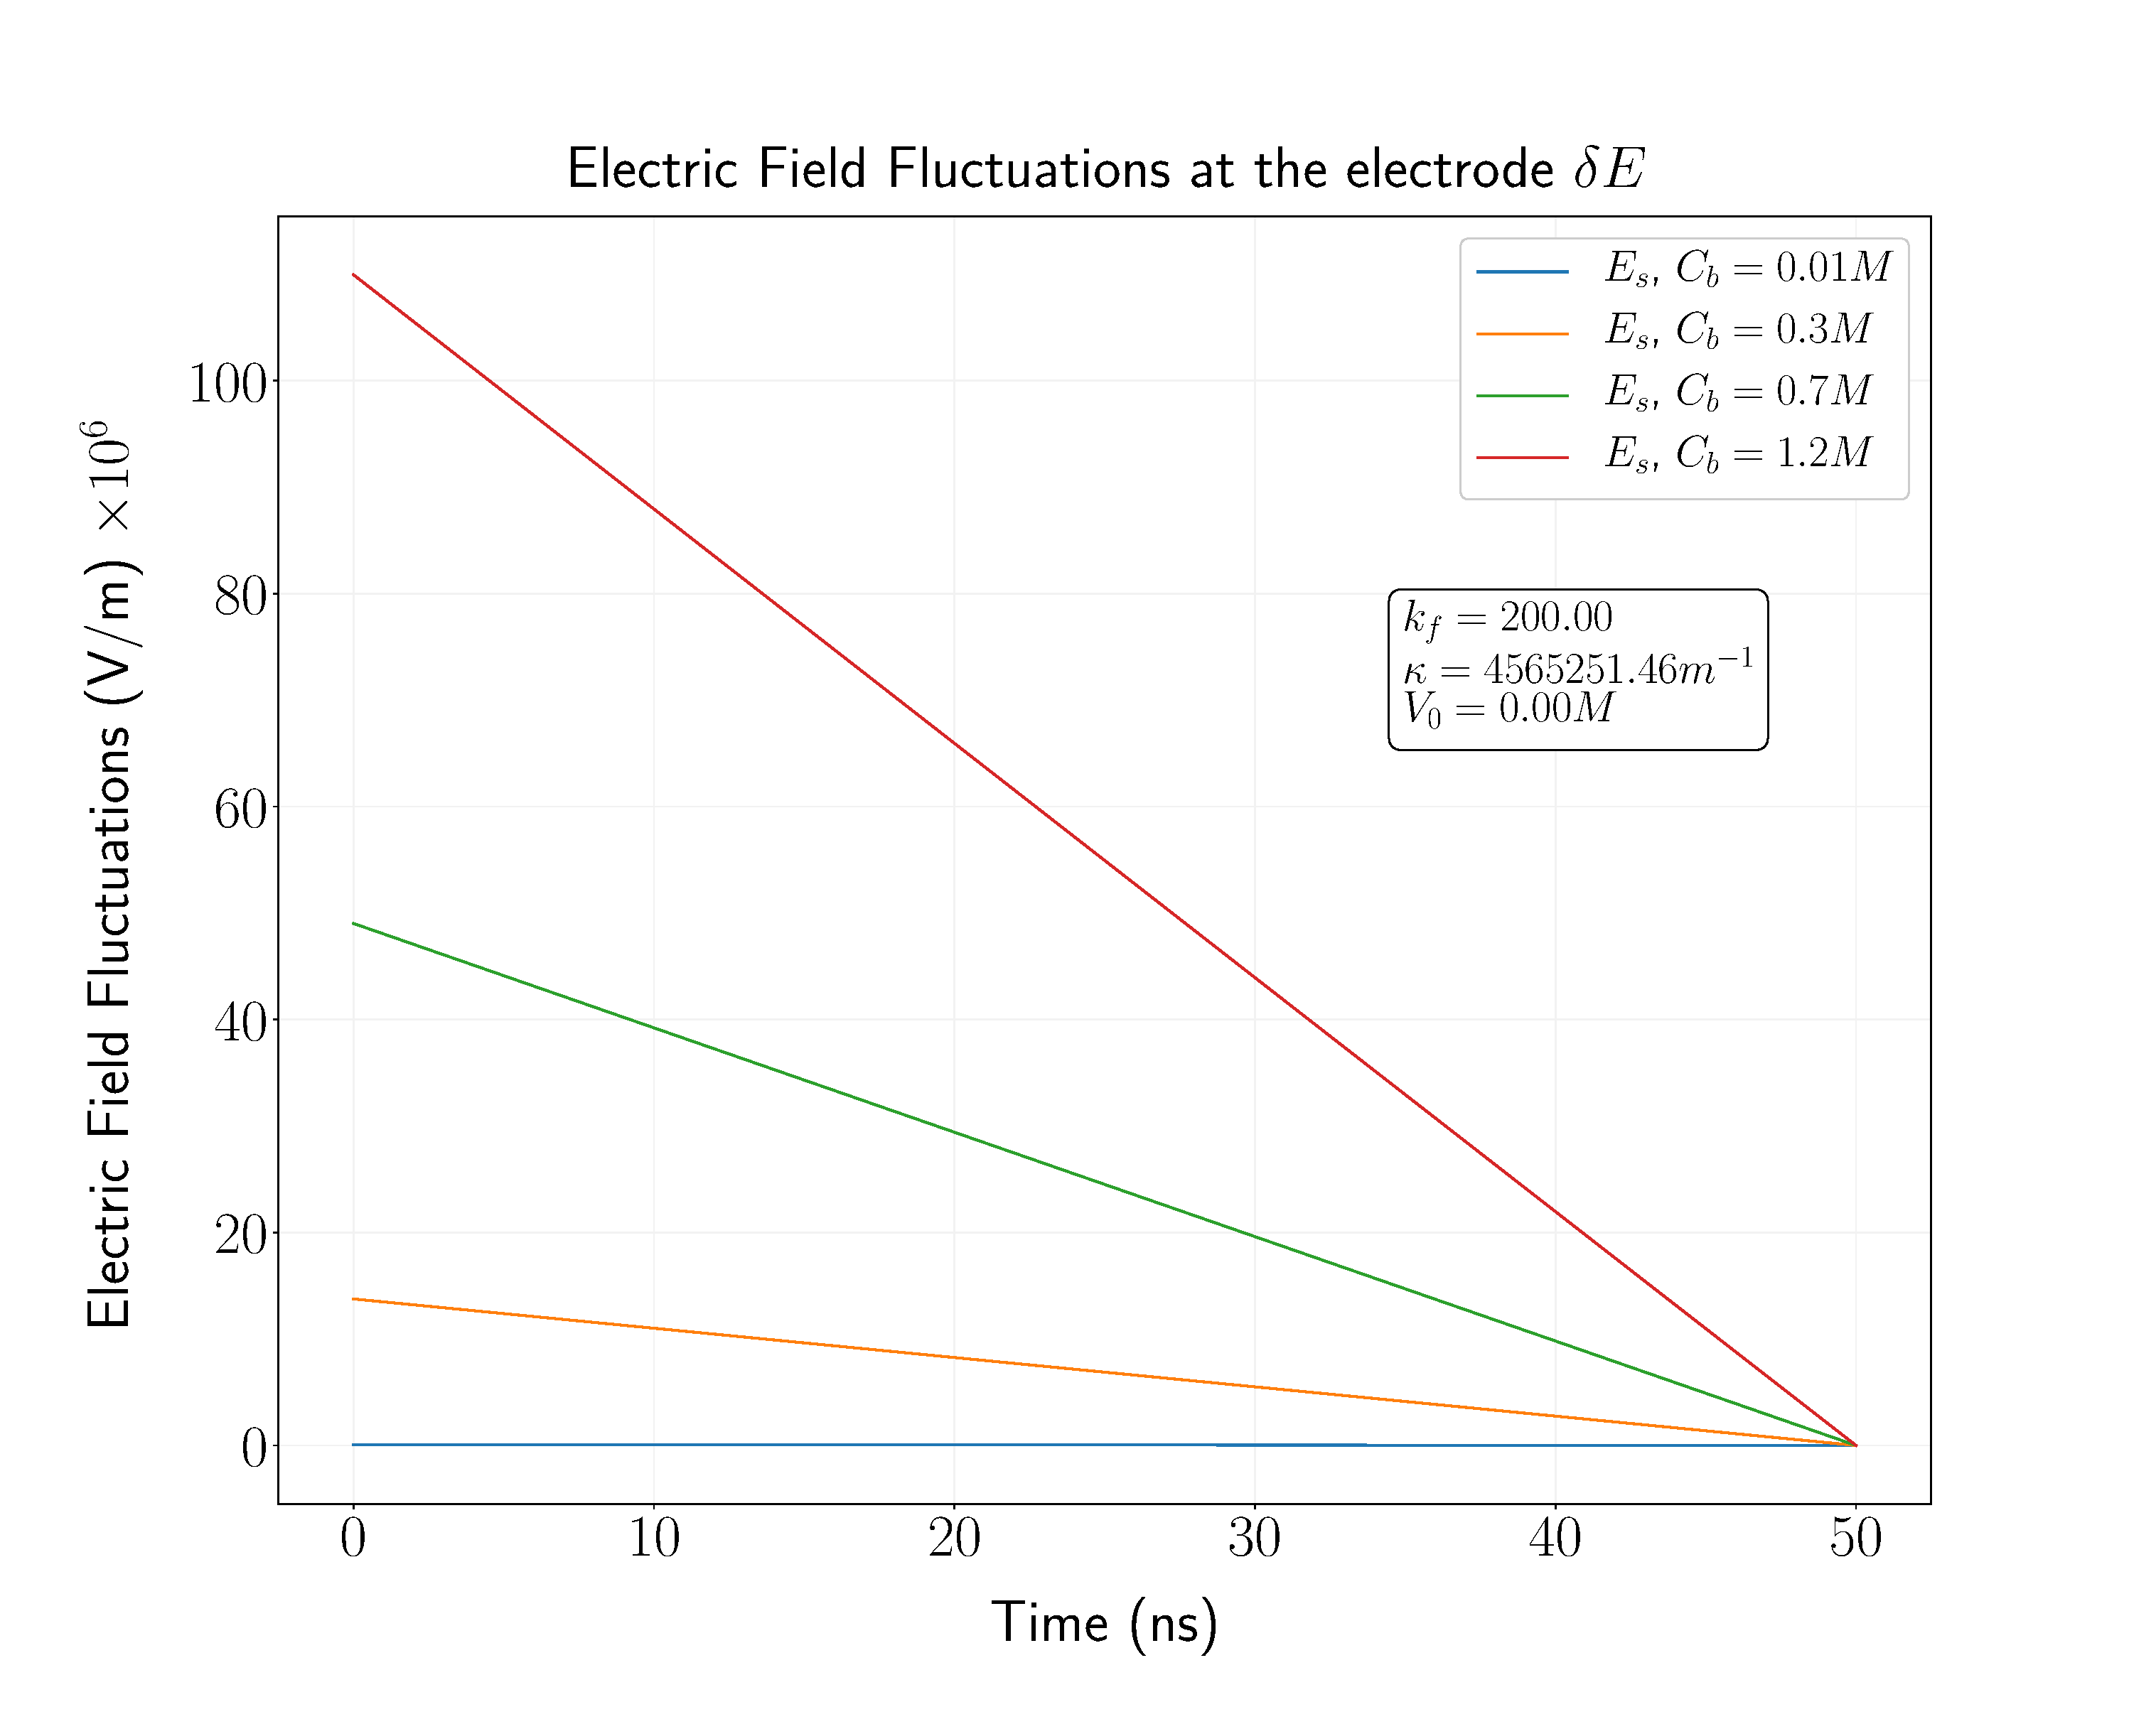
\includegraphics[width=\textwidth]{surfaceDeltaE.eps}
\caption{Electric field fluctuations at the electrode.}
\label{fig:nernts-no-field}
\end{figure}


\newpage




%\section{Forced System Setup}

\subsection{Time Evolution}



\begin{figure}[htbp]
\centering
\textbf{Electric Field In The Diffusion Problem With Nernst Interaction.}\par\medskip
\begin{subfigure}{.5\linewidth}
\centering
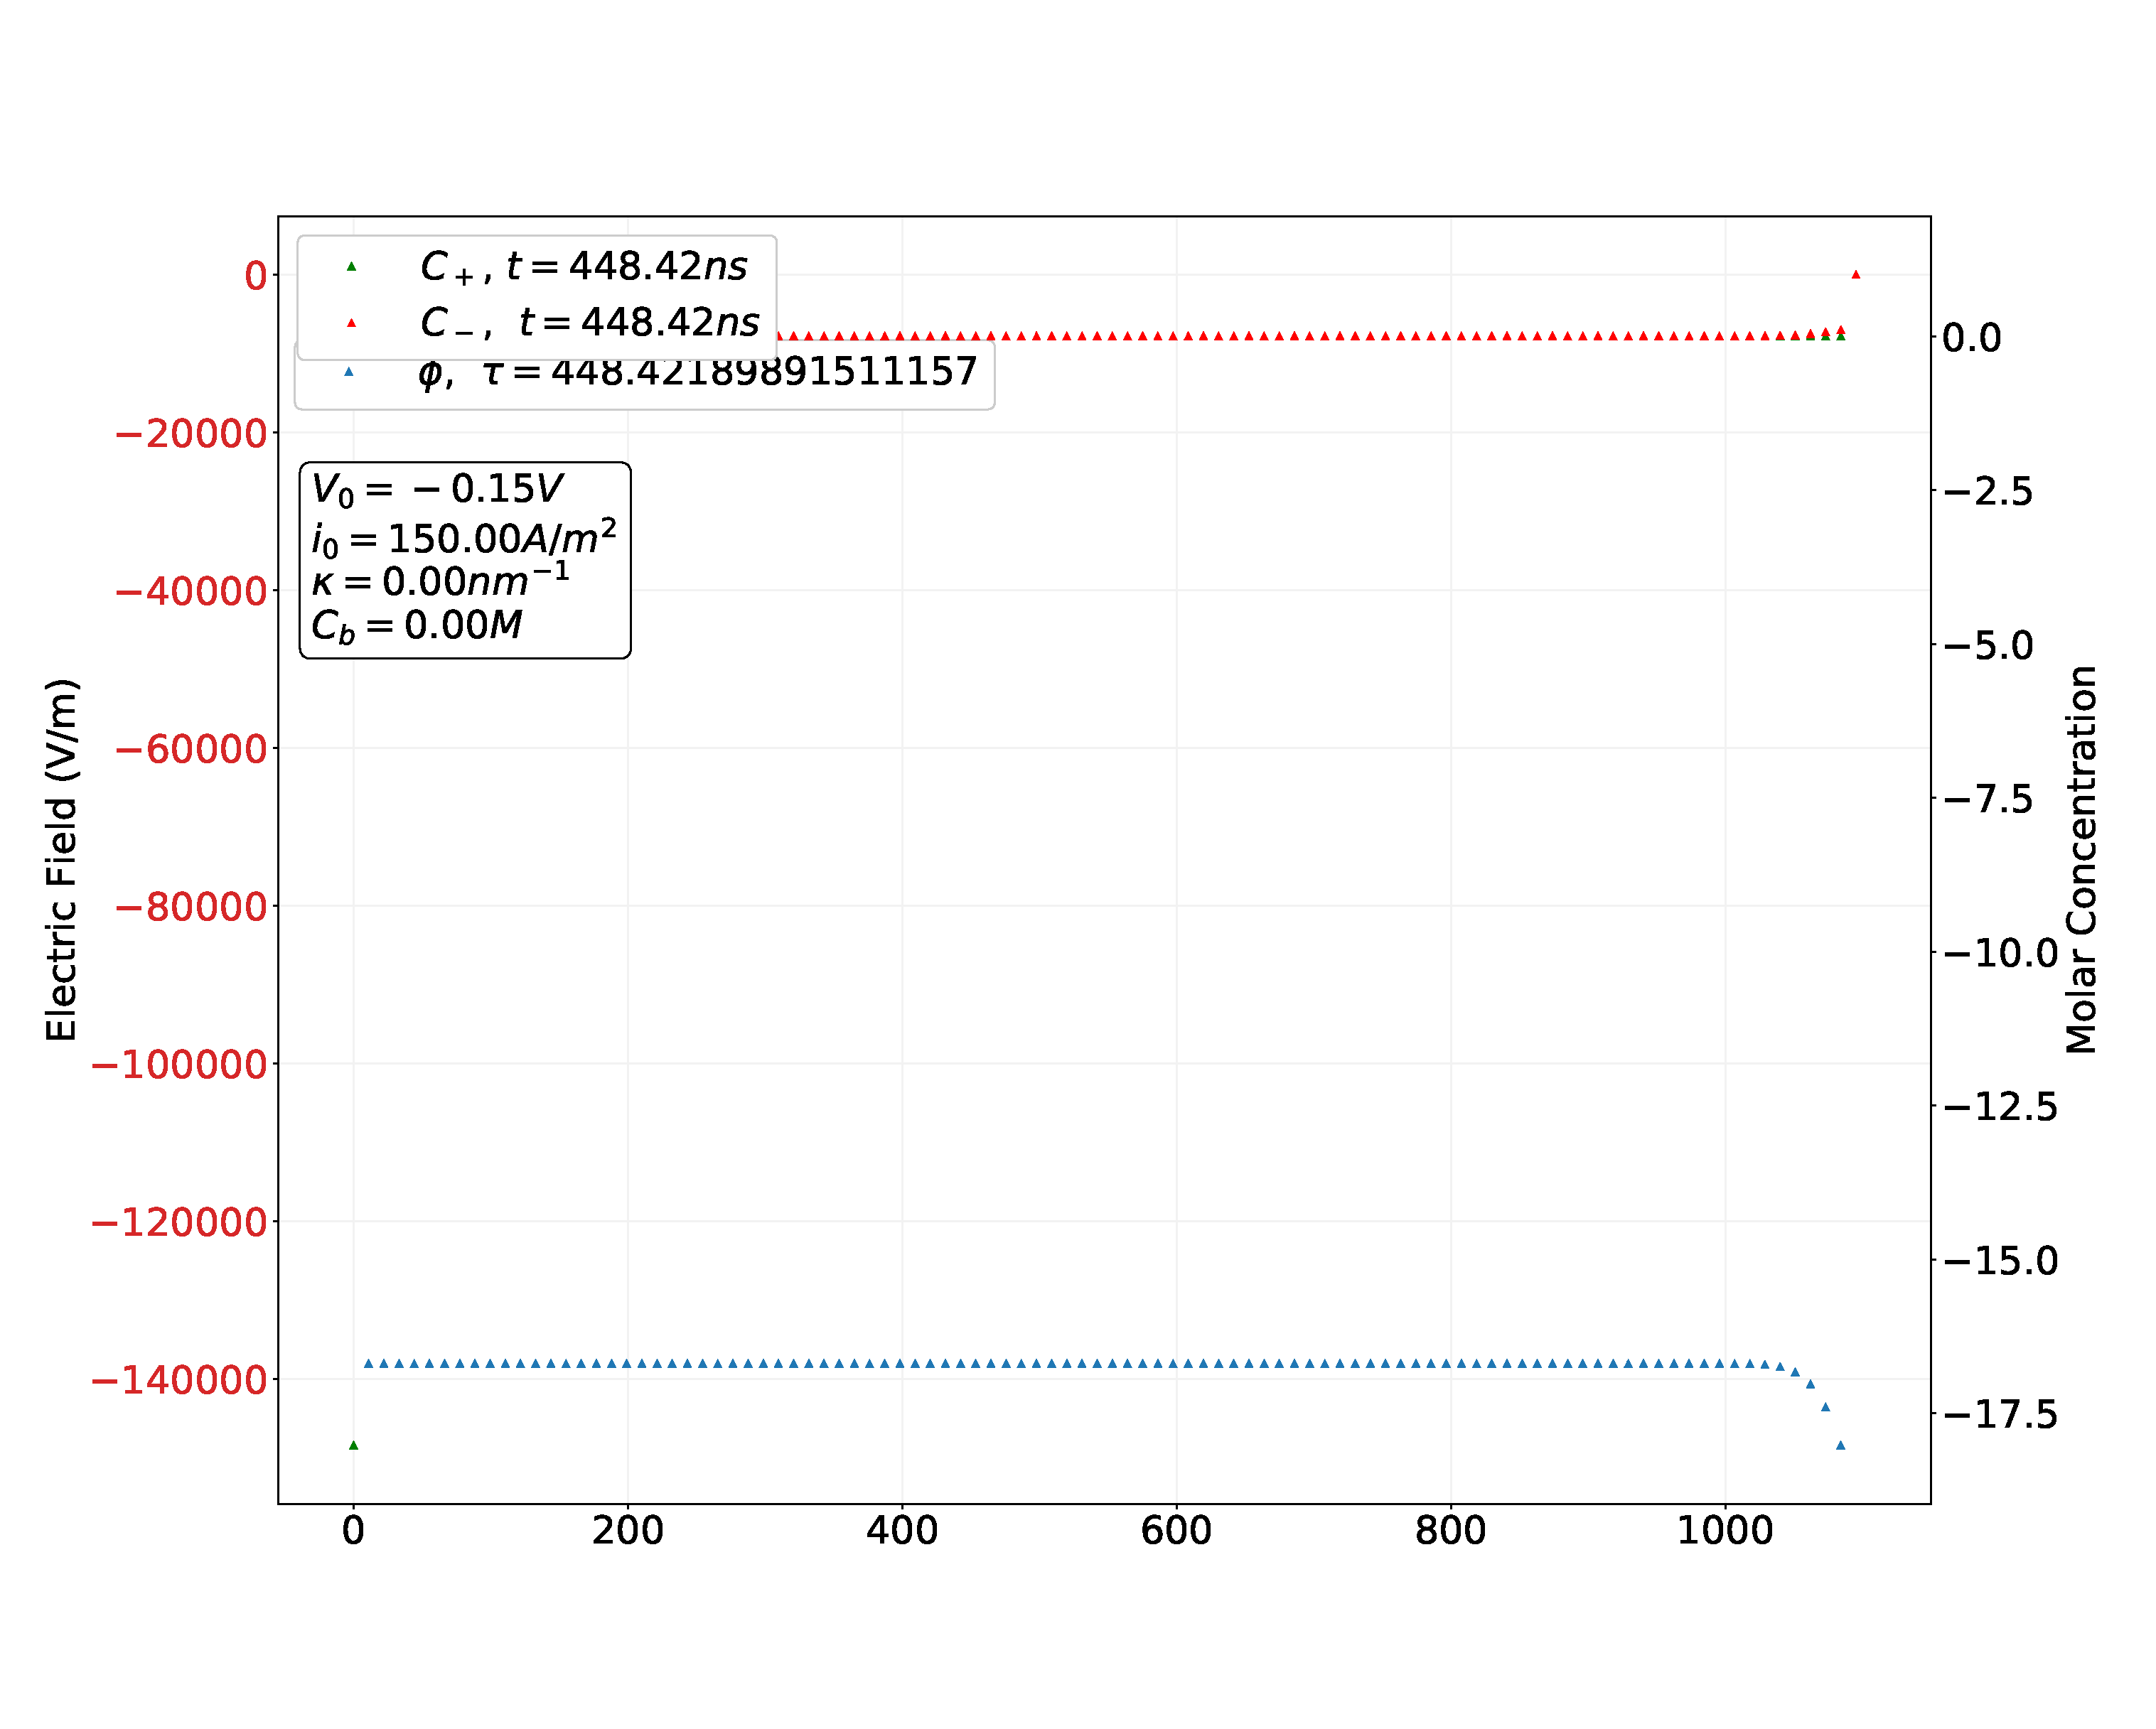
\includegraphics[width=\textwidth]{forced-current-nernstE0.eps}
\caption{}
\label{fig:ef1}
\end{subfigure}%
\begin{subfigure}{.5\linewidth}
\centering
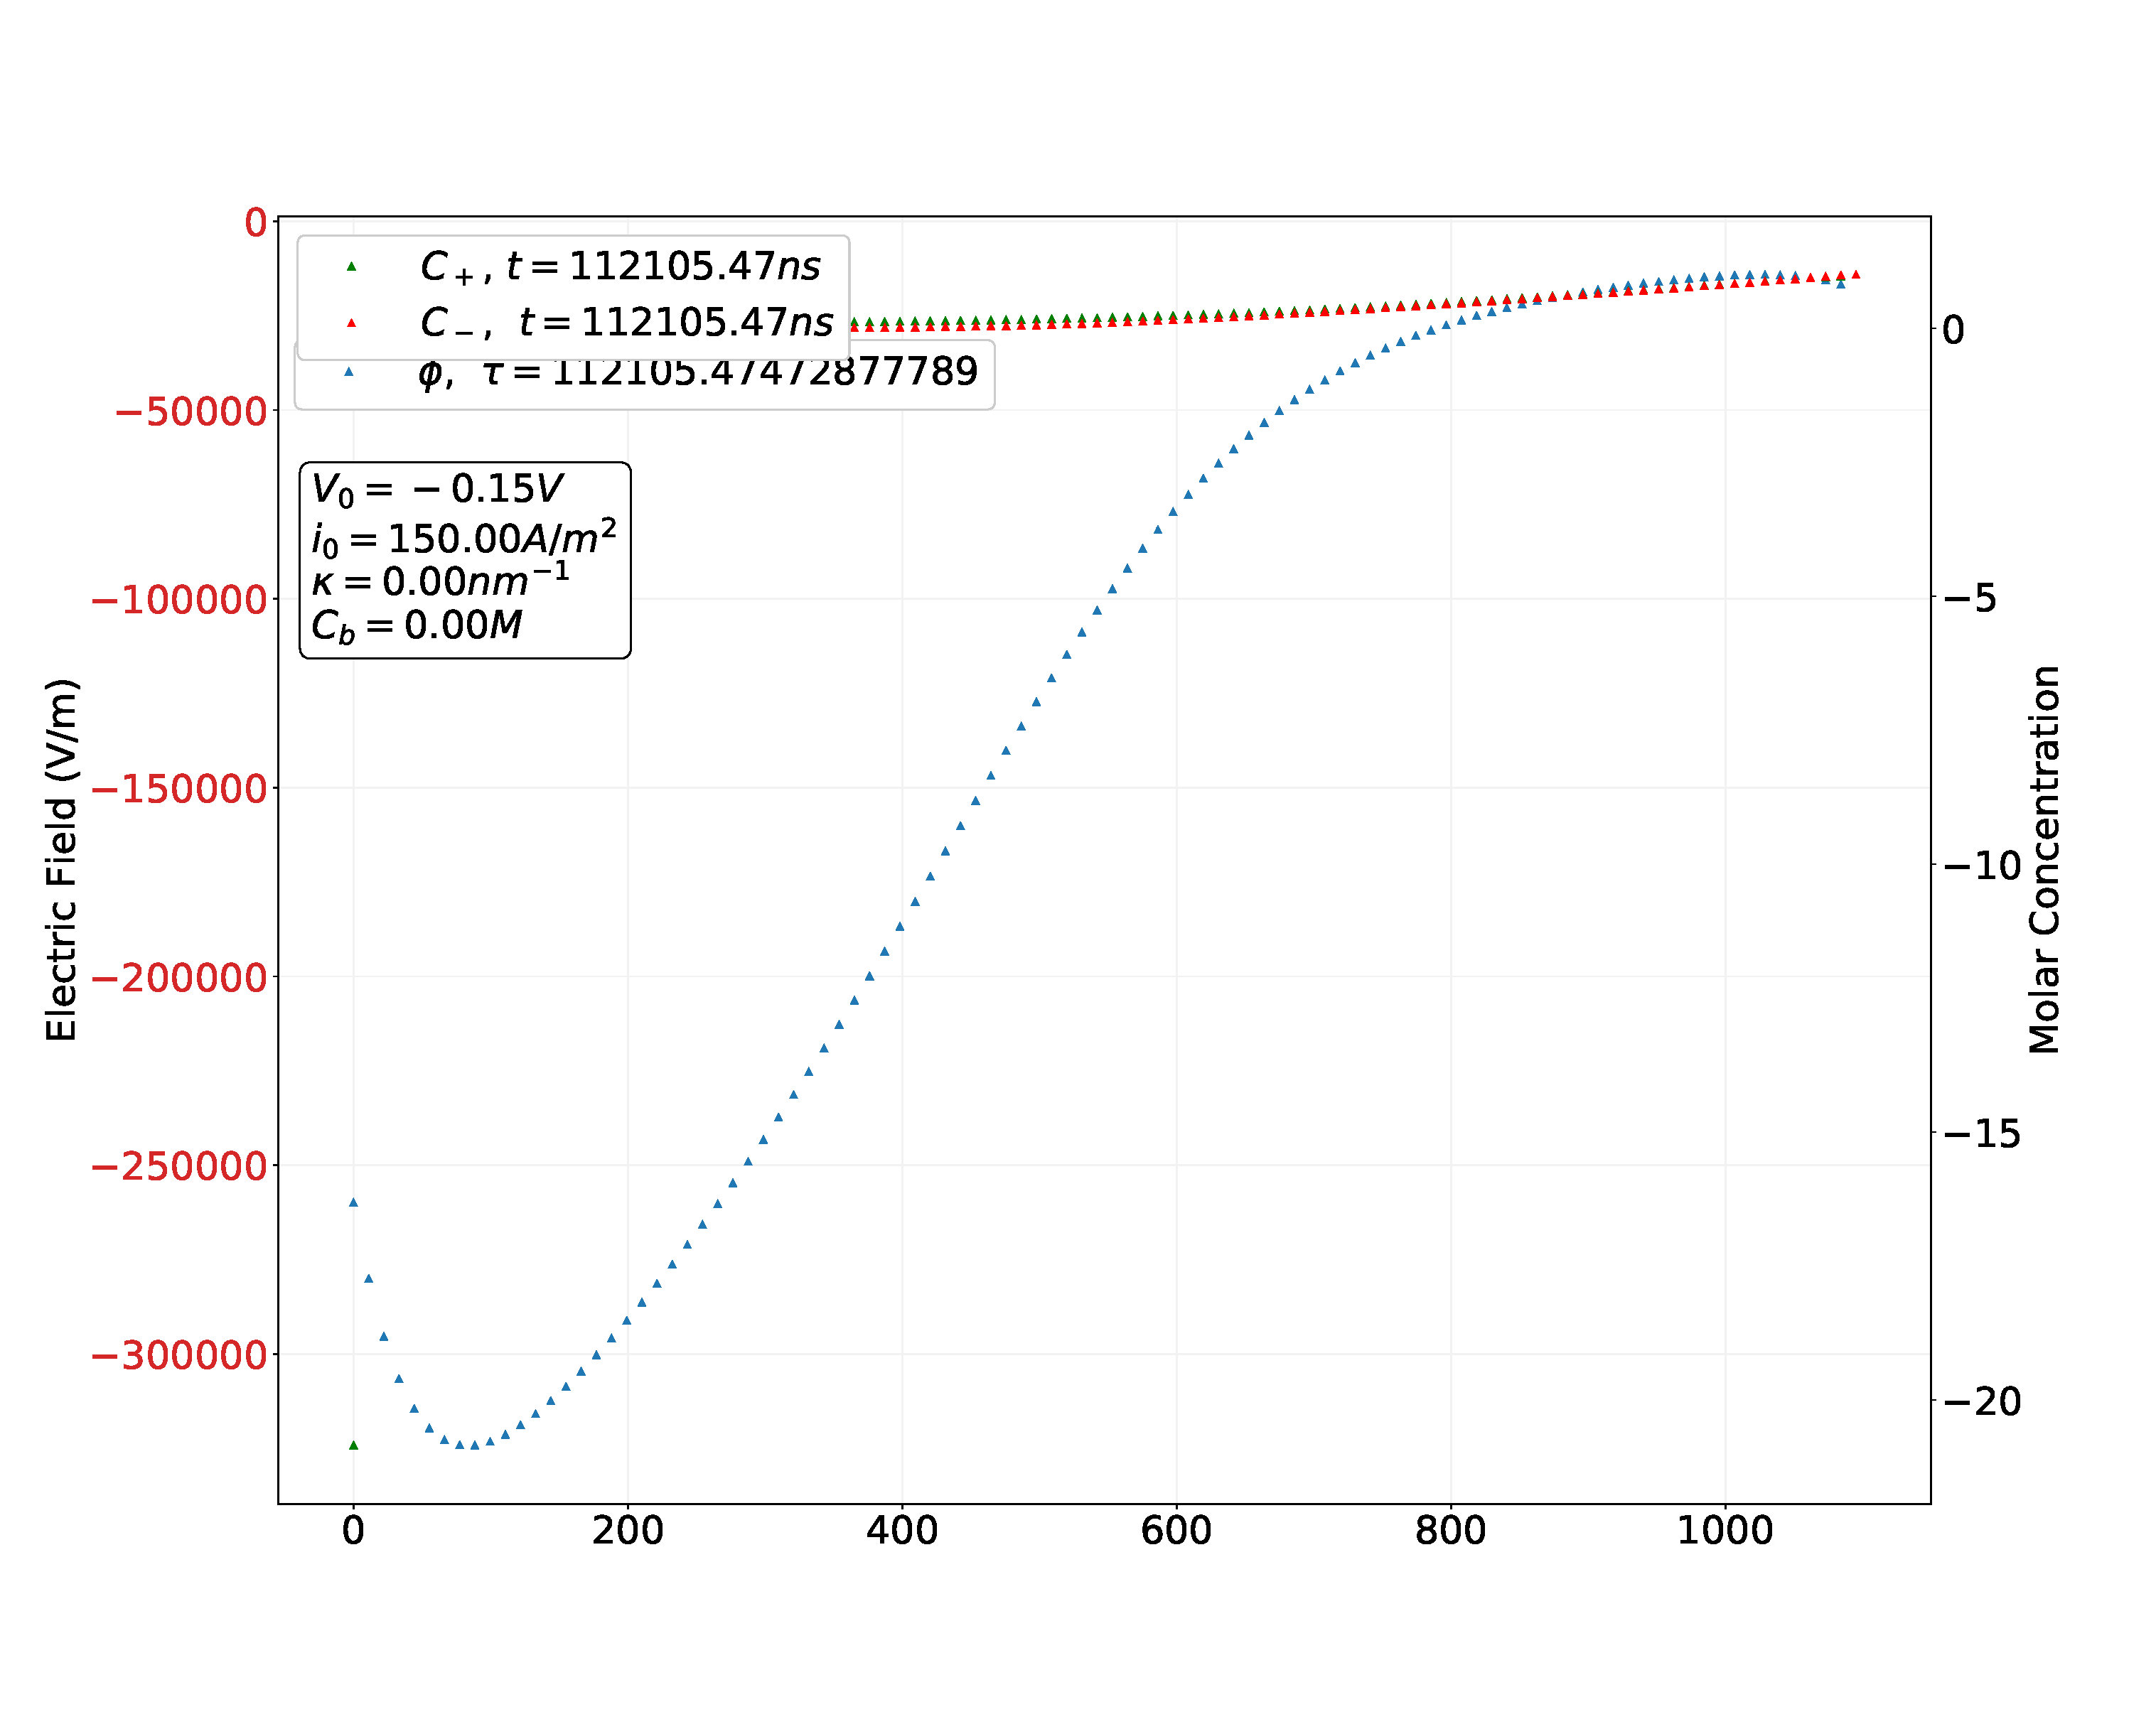
\includegraphics[width =\textwidth]{forced-current-nernstE1.eps}
\caption{}
\label{fig:ef2}
\end{subfigure}\\[1ex]
\begin{subfigure}{\linewidth}
\centering
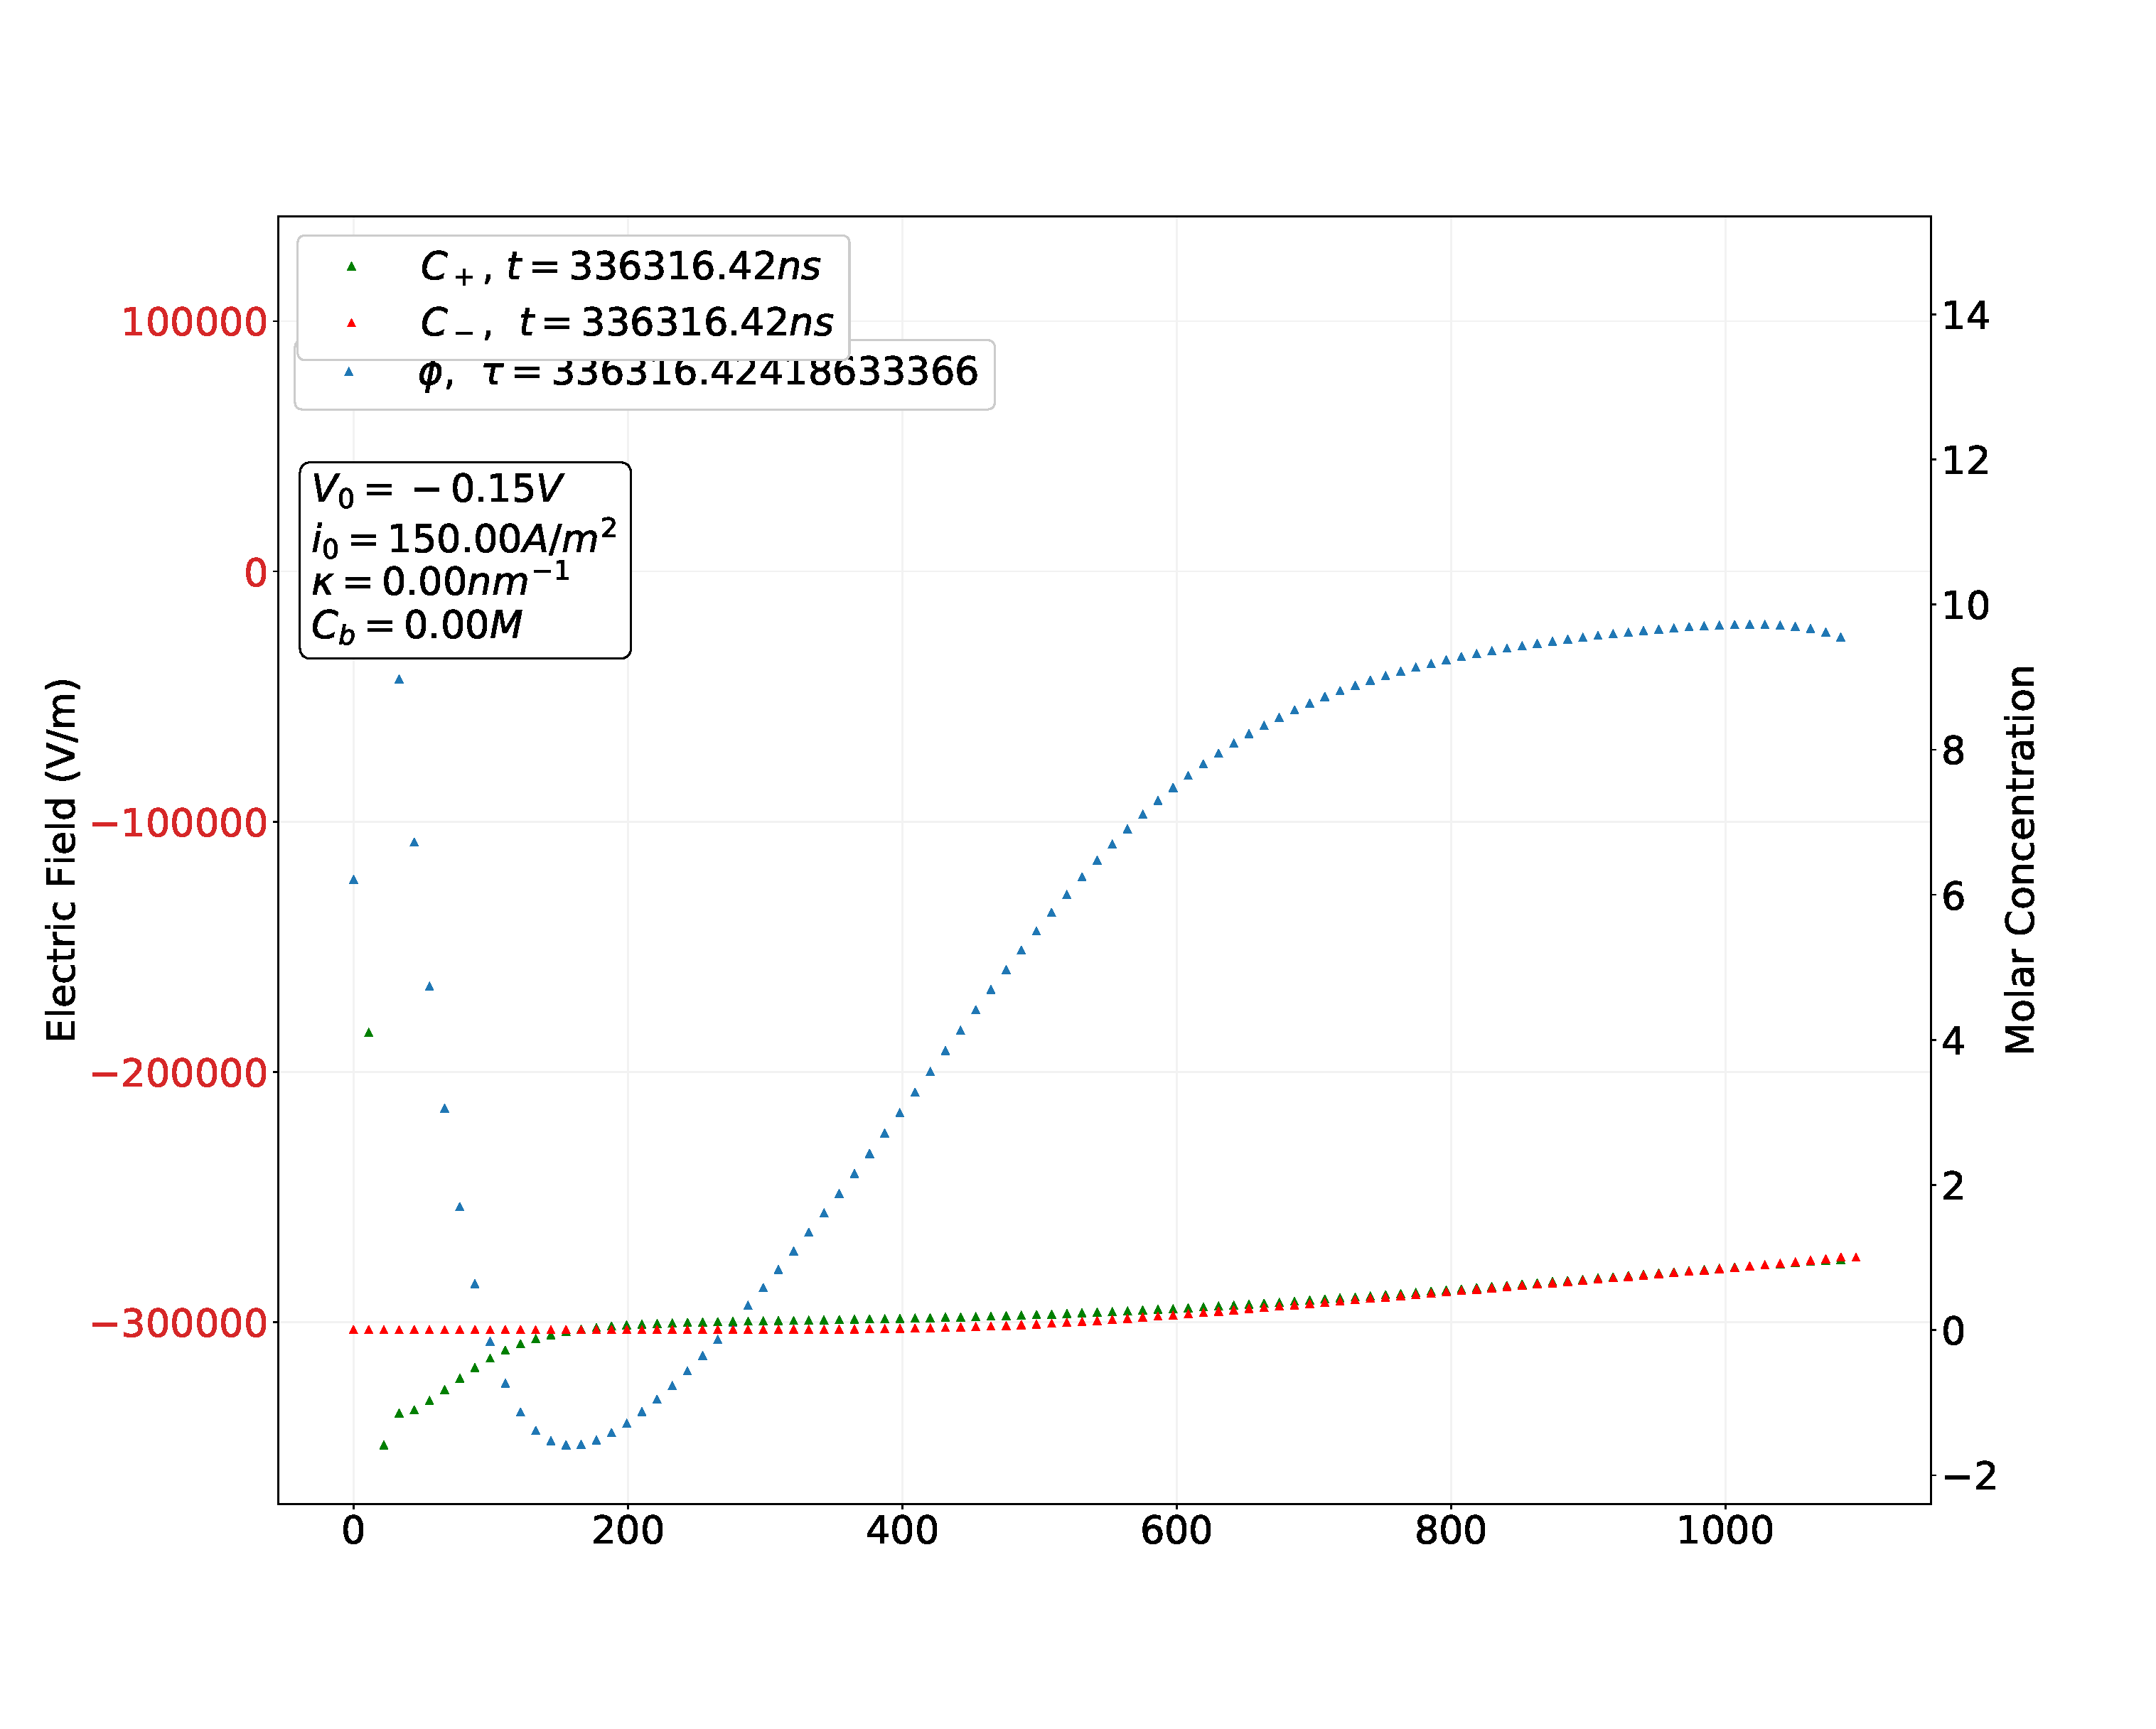
\includegraphics[width =0.5\textwidth]{forced-current-nernstE2.eps}
\caption{}
\label{fig:ef3}
\end{subfigure}
\caption{Electric field and concentration of $Cu^{+2}$ (green dots) and $SO_4^{-2}$ (blue dots) at (a) $t = 0.448 ns$, (b) $t = 2.24 ns$ and (c) $t = 4.44 ns$}.
\label{fig:test}
\end{figure}

\begin{figure}[htbp]
\centering
\textbf{Electric Potential In The Diffusion Problem With Nernst Interaction.}\par\medskip
\begin{subfigure}{.5\linewidth}
\centering
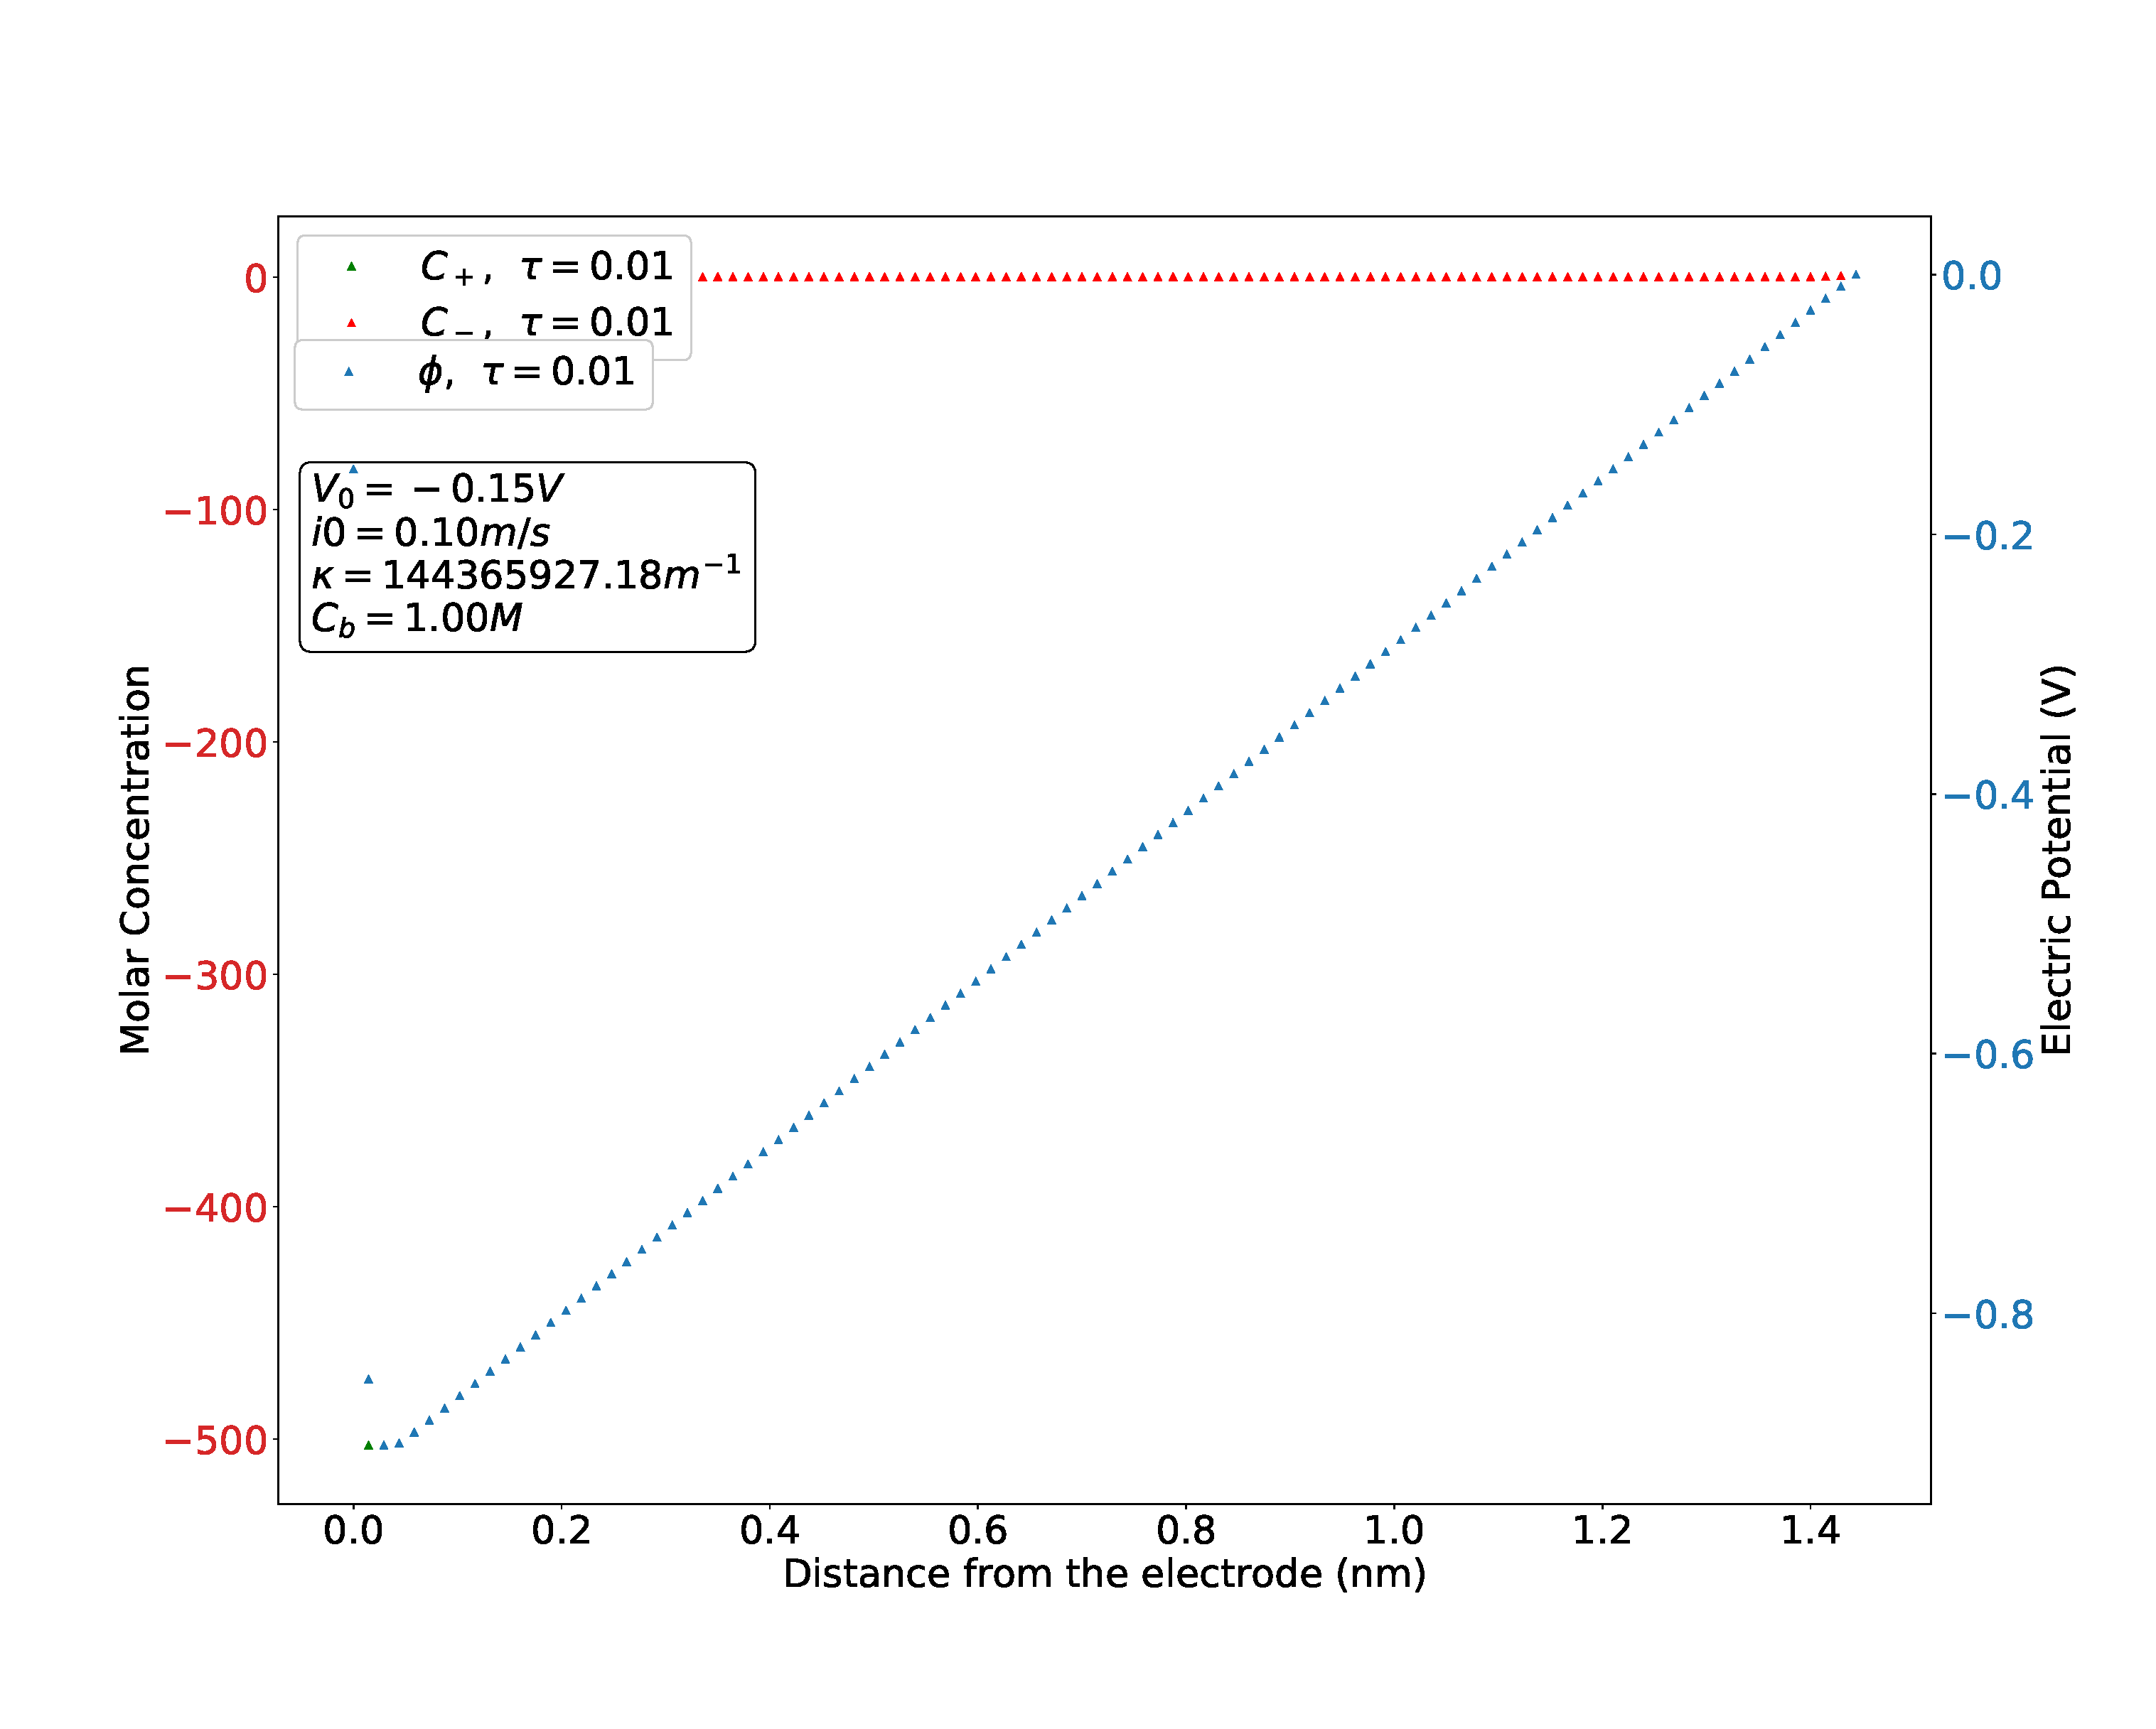
\includegraphics[width=\textwidth]{forced-current-nernstphi0.eps}
\caption{}
\label{fig:ef1}
\end{subfigure}%
\begin{subfigure}{.5\linewidth}
\centering
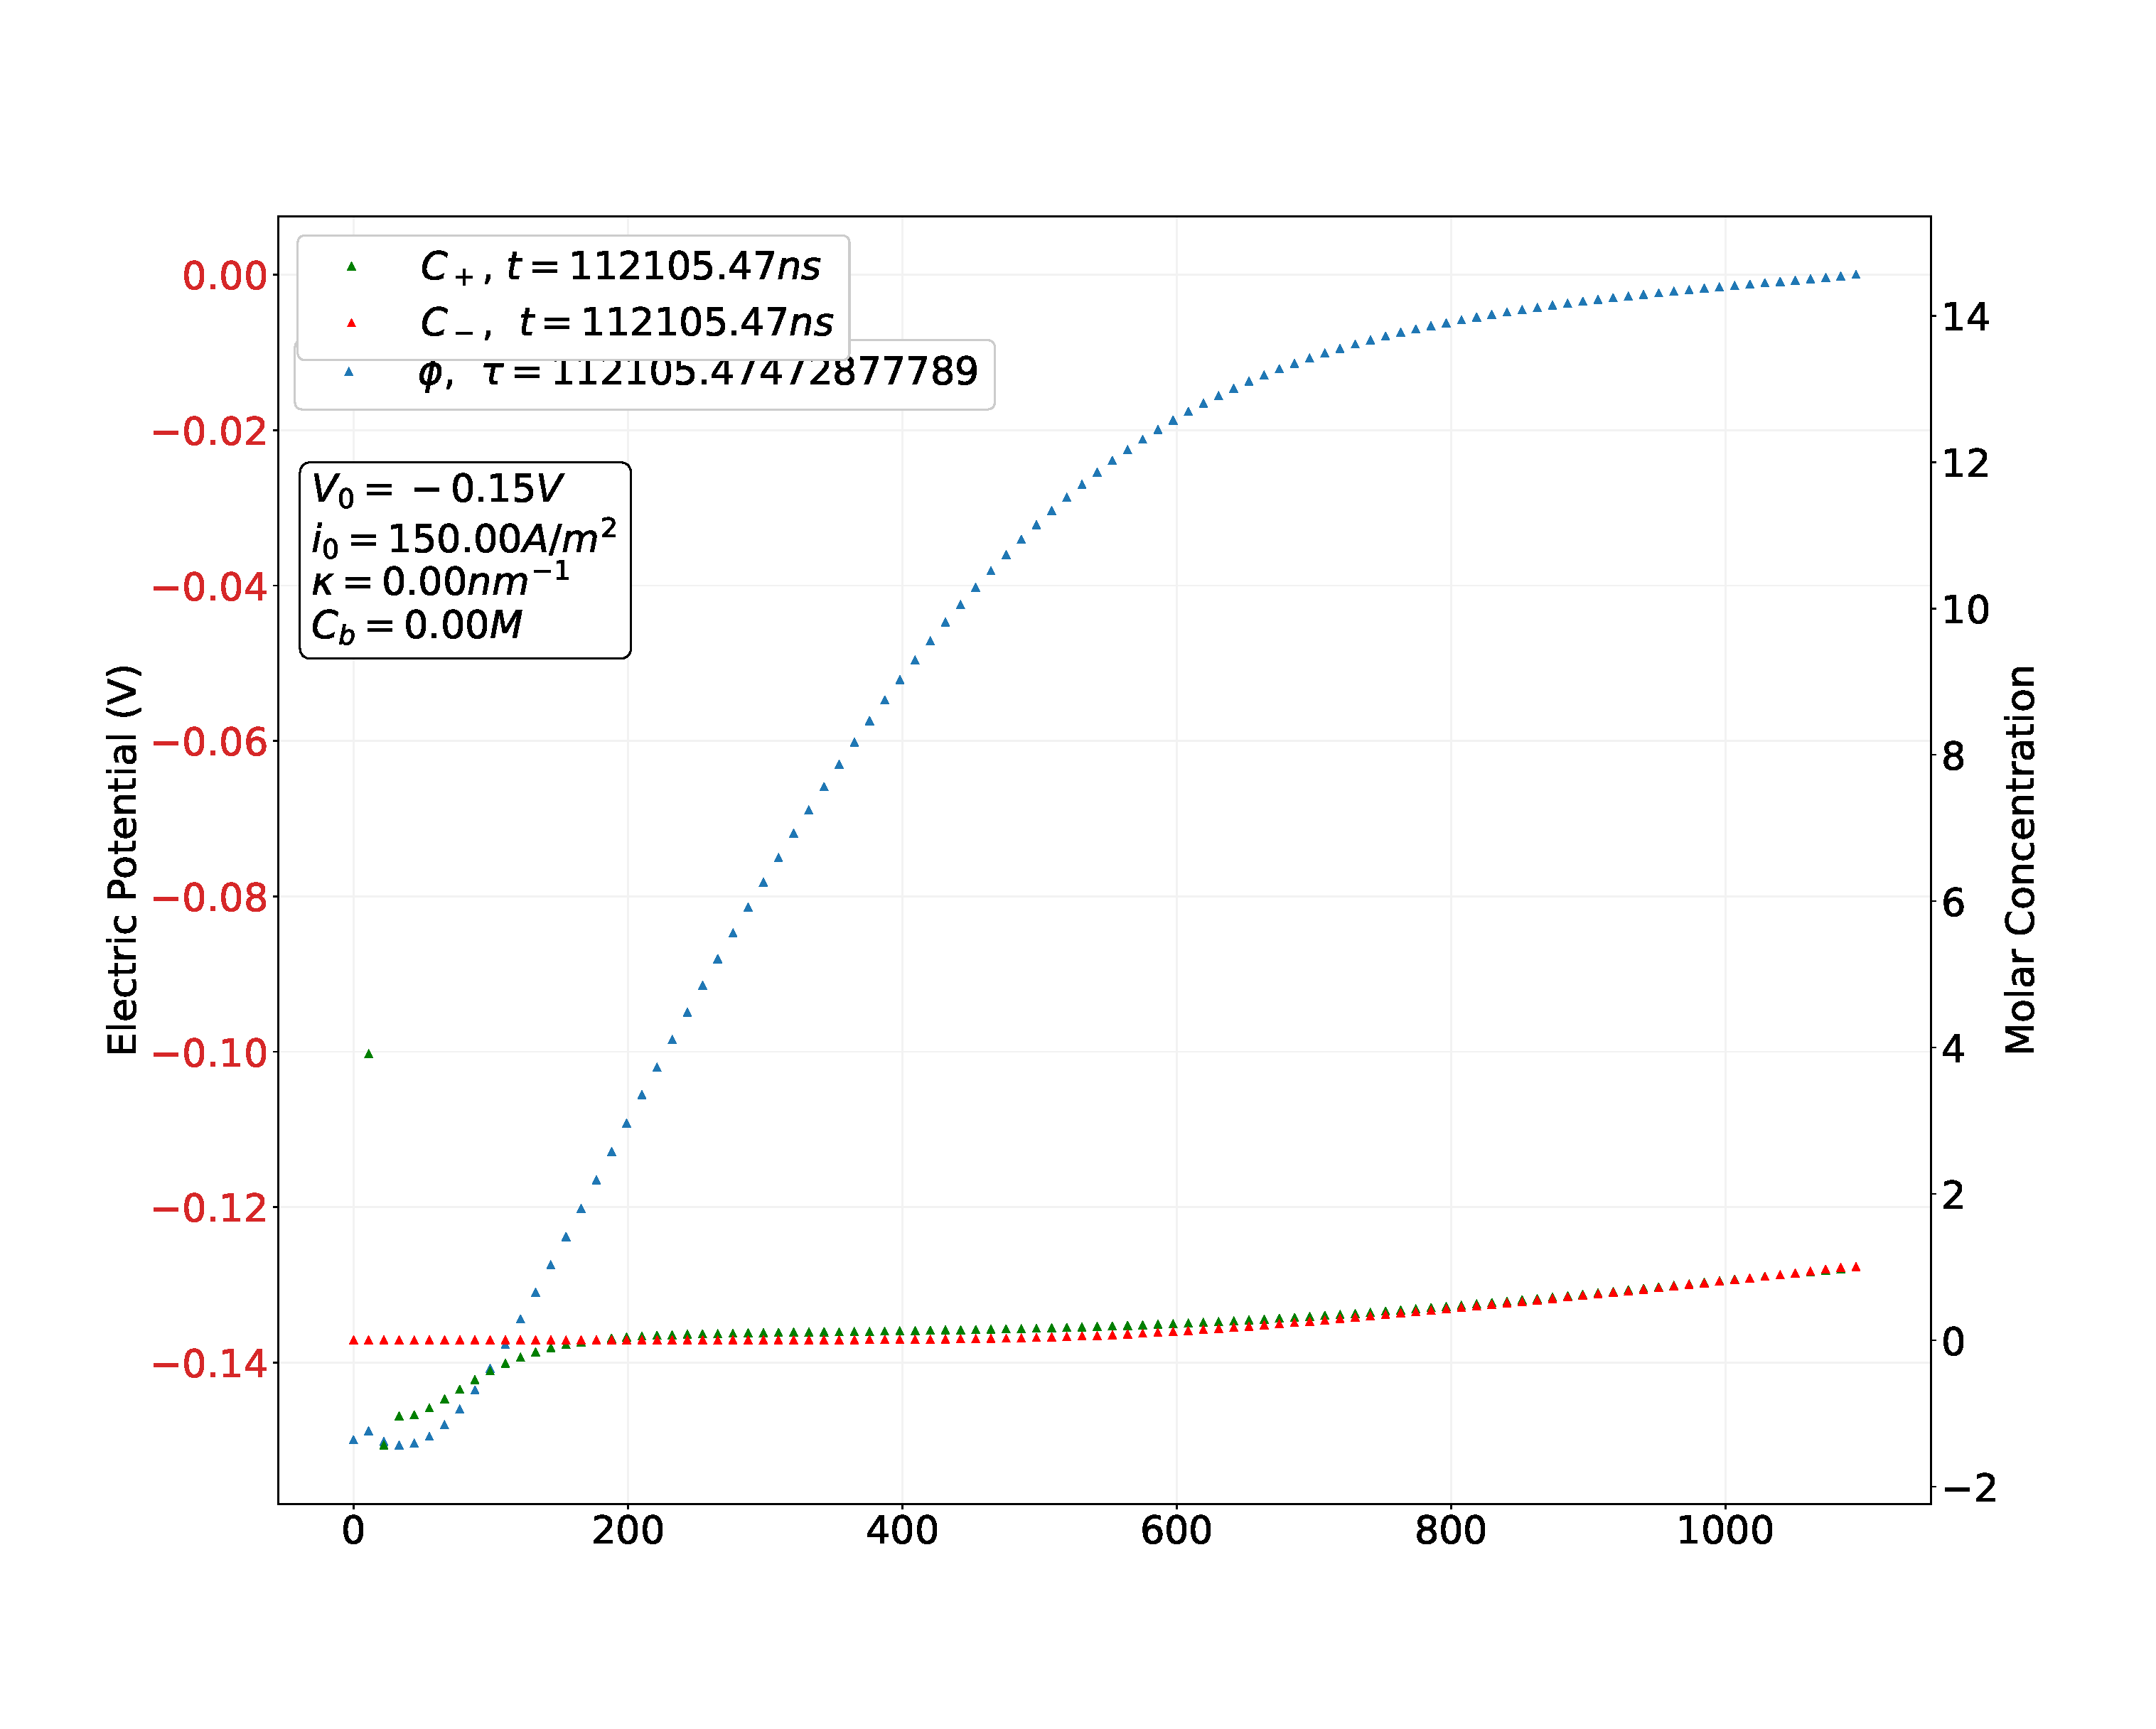
\includegraphics[width =\textwidth]{forced-current-nernstphi1.eps}
\caption{}
\label{fig:ef2}
\end{subfigure}\\[1ex]
\begin{subfigure}{\linewidth}
\centering
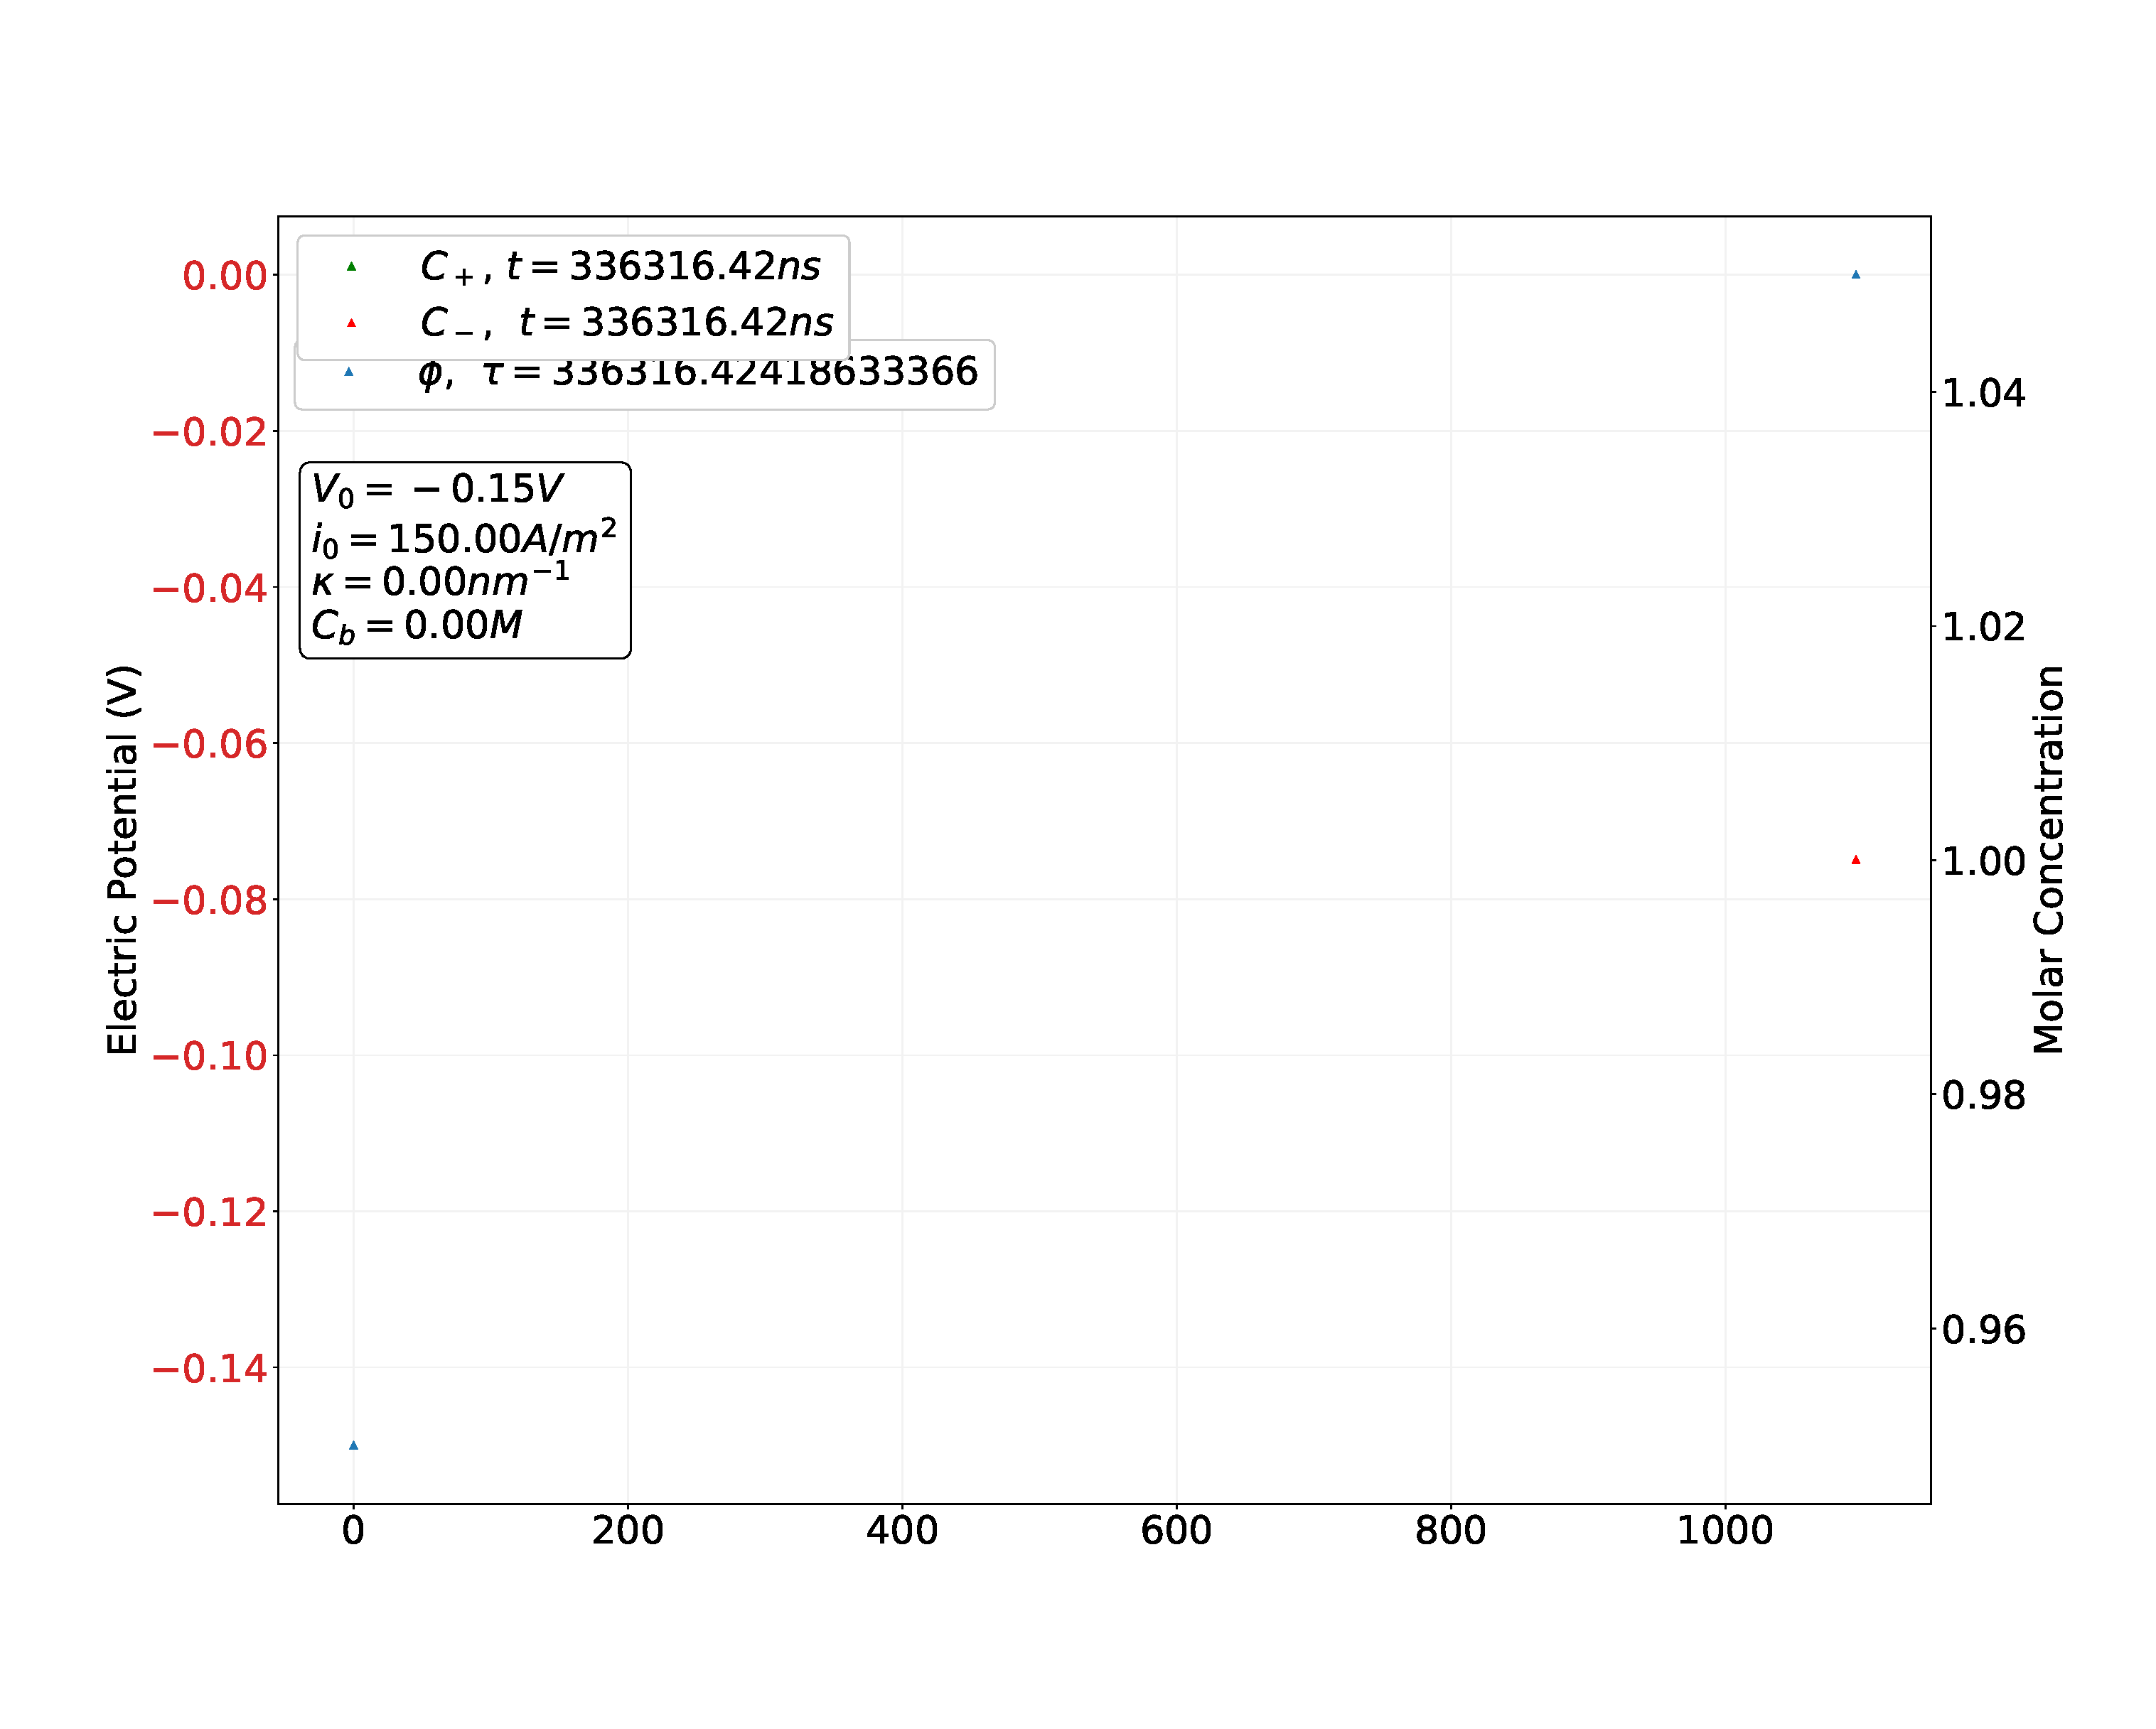
\includegraphics[width =0.5\textwidth]{forced-current-nernstphi2.eps}
\caption{}
\label{fig:ef3}
\end{subfigure}
\caption{Electric potential in volts and molar concentration of $Cu^{+2}$ (green dots) and $SO_4^{-2}$ (blue dots) at (a) $t = 0.448 ns$, (b) $t = 2.24 ns$ and (c) $t = 4.44 ns$}
\label{fig:test}
\end{figure}

\newpage

%\subsection{Electric Field At The Surface}

%\newpage
%\subsection{Electric Field Fluctuations At The Surface}





\chapter{Conclusions}
\section{Conclusions}

One of the objectives of this work (outlined in Sec. \ref{sec:context}) was to provide a model to connect surface electric field fluctuations with the bulk concentration, which is one of our boundary conditions for our system. Using methods described in \ref{ch:results-analysis}, we have found through both numerical and analytical results that the surface electric field is proportional to the square root of the bulk concentration, that is

\begin{align}
	E_{surface}(t) \propto \sqrt{C_b}.
\end{align}

In terms of the strategy to simulate the copper electro-refining process, Fig. \ref{fig:efield-noise-fit} suggests that electric field noise can be modeled using the steady state solution alone. This is because the relaxation time (with the parameters used in \ref{sec:analysis-efield}, which are all sensible values for this type of processes) is about $50 ns$ (see Fig \ref{fig:efield-noise-fit}), which compared with the time scale this processes take (hours to days \cite{schlesinger}) is neglectible.

Also, the ionic force \ref{eq:ionic-force} gives us a measure of the screening length of the electrolyte. In the context of building an NV-Center, nano-diamond based sensor to measure the electric field fluctuations, special care has to be taken in positioning the sensor. This because, for the electro-refining process parameters the ionic force $\kappa$ of the order of nanometers to hundred of nanometers.

A final conclusion is that this work and the results obtained in it can be used for optimized control over the process of electro-refinement of copper.

\section{Further Work}

This work offers a set of results which can be used to obtain insights into the electro-refinement of copper process. To gain further insight work still needs to be done. In particular, we are interested in the stochastic nature of the electric field fluctuations at the surface. Nevertheless, our results are determinant and continuos. This is because we are dealing with average quantities, and the evolution of these quantities as a whole. A stochastic component can be introduced to study the evolution of the system, which is interesting as an approach to simulating data obtained by the sensor or even calibrate the sensor according to the simulated data. 

The stochastic component can be introduced in two ways. Firstly, we can introduce fluctuations of the boundary condition of the problem. The convenience of this approach is its ease of implementation. Basically, the equations remain the same and we make the boundary conditions to fluctuate around the mean value following a distribution. 

The second approach is to model the microscopic equations and simulate the distribution of particles in the system through the master equation method. Both of these approaches would be interesting to investigate further.


\section{Code}

The numerical methods used in this work where modified from \cite{kiusalaas} and are written in Python 3. These methods such as Finite Difference methods, Runge-Kutta methods and other complementary methods are available on GitHub \textit{https://github.com/atescobar/NumericMethods}. The code of the simulation itself can be requested through personal email to \textit{atescobar@uc.cl}.


\begin{appendices}
\chapter{Calculations Of Chapter \ref{ch:2}}
\section{Potential to first order in the current}
\label{appendix:first-order-potential}
Now we need to solve Eq. \ref{eq:concentration-diff-first6}
\begin{eqnarray}
\frac{\partial^2  \Phi^{(1)}}{\partial \xi^2} &=& -(C^{(1)}_{+}(\xi)-C^{(1)}_{-}(\xi)).
\end{eqnarray}

Expanding, we have 

\begin{eqnarray}\nonumber
\frac{\partial^2  \Phi^{(1)}}{\partial \xi^2} &=& -C^{(1)}_{+}(\xi)\\
&=&- \frac{1}{\kappa} \qty{\xi_\delta-\xi-\frac{2}{\gamma}}\tanh^2\qty{\frac{\xi-\xi_0}{2}}-\frac{2}{\kappa}\tanh\qty{\frac{\xi-\xi_0}{2}}.
\end{eqnarray}


Integrating twice and using the fact that $\Phi'^{(1)}(\xi_\delta) = 0$, $\Phi^{(1)}(\xi_\delta) = 0$ we obtain

\begin{eqnarray}
\Phi'^{(1)}(\xi) = \frac{1}{\kappa} \qty{A + B\xi + C\xi^2 + D \tanh{\frac{\xi-\xi_0}{2}}+E\xi\tanh{\frac{\xi-\xi_0}{2}}} .
\end{eqnarray}


And 

\begin{eqnarray}
\Phi^{(1)}(\xi) = -\frac{1}{\kappa} (A(\xi_\delta - \xi) + \frac{B}{2}(\xi_\delta^2-\xi^2) + \frac{C}{3}(\xi_\delta^3 - \xi^3) + \\
D\log\bigg|\frac{\cosh{\frac{\xi_\delta-\xi}{2}}}{\cosh{\frac{\xi-\xi}{2}}}\bigg| + E \qty{\xi_\delta\log|\cosh\qty{\frac{\xi_\delta-\xi_0}{2}}-\xi\log|\cosh\qty{\frac{\xi-\xi_0}{2}}}-EI_\delta(\xi),
\end{eqnarray}


where

\begin{eqnarray*}
	A = 2\gamma\xi_\delta - \frac{2\xi_\delta}{\gamma} - 2 \gamma - \frac{\xi_\delta^2}{2},\\
	B = -\qty{\xi_\delta -\frac{2}{\gamma}},\\
	C = \frac{3}{2}\\
	D = -2 \qty{\xi_\delta - \frac{2}{\gamma}},\\
	E = 2,\\
	\gamma = \tanh\qty{\frac{\xi_0}{2}},
\end{eqnarray*}

and

\begin{align}
	I_\delta(\xi) = \int_\xi^{\xi_\delta} \log\bigg|\cosh\qty{\frac{\xi-\xi_0}{2}}\bigg| d\xi.
\end{align}




This integral must be evaluated numerically for each value of $\xi$. In order to do this, we use the Simpson Rule. Fig. \ref{fig:analytic-results} shows the potential to first order in the current alongside with the zero order potential. 
\chapter{Calculations And Numerical Analysis Of Chapter \ref{ch:3}}
\section{Analytic Solution To The Diffusion-Only Problem}
\label{appendix:analytic-diff-only}
In this section we solve the diffusion problem with homogenous boundary conditions by transforming system

\begin{align}
\frac{\partial C}{\partial t} &= D \frac{\partial^2 C}{\partial x^2}
\end{align}

\begin{align}
	C(\delta, t) = -C_b, \\
	 J(0, t) &= D\frac{\partial C}{\partial x}\big|_{x=0} = 0.
\end{align}

into the dimensionless system

\begin{align}
	\rho(x,t) &= \frac{C(x,t) - C_b}{C_b}.
	\label{eq:rho-def}
\end{align}

This yields the following PDE

\begin{align}
\frac{\partial \rho}{\partial t} &= D \frac{\partial^2 \rho}{\partial x^2},\\
\label{eq:diffusion-1d}
\end{align}


The border conditions for the new function \ref{eq:rho-def} are

\begin{align}
	\rho(\delta, t) = -1, \\
	C_b D\frac{\partial \rho}{\partial x}\big|_{x=0} &= J(0, t) = 0.
\end{align}


We will solve this equation using the method of separation of variables. Let

\begin{align}
	\rho(x,t) = g(t)f(x).
\end{align}

We get the following two equations for $g(t)$ and $f(x)$


\begin{align}
	g'(t) + \lambda g(t) &= 0,\\
	f''(x) + \frac{\lambda}{D} f(x) &= 0.
\end{align}

$\lambda$ is a positive constant, due to boundary conditions. The solution to these equations are

\begin{align}
	g(t) =& g_{-}(0)e^{-\lambda t},\\
	f(x) =& F^1_{-,\lambda}\cos\qty{{\sqrt{\frac{\lambda}{D}} x}} + F^2_{-,\lambda}\sin\qty{\sqrt{\frac{\lambda}{D}} x},
\end{align}

where $F^1_{-,\lambda}$, $F^2_{-,\lambda}$ and $G_{-,0}$ are constants dependent on the parameter $\lambda$, which is yet to be determined. Border conditions \ref{eq:diffusion-1d} yield $B_{-,\lambda} = 0$. We get the general solution,


\begin{align}
	\rho(x,t) = \sum_{\lambda} A_\lambda e^{-\lambda t} \cos\qty{\frac{\lambda}{D} x},
\end{align}

where $A_{-,\lambda} = g(0)F^1_{-,\lambda}$. is a constant. Considering the border condition at $x=\delta$, we can determine the value of $\lambda$,


\begin{align}
\label{eq:general-expresion-rho}
	\rho(x=\delta,t) = \sum_{\lambda} A_\lambda e^{-\lambda t} \cos\qty{\frac{\lambda}{D} \delta} = 0.
\end{align}

The only way (unless $A_{-,\lambda} = 0$, in which case we get the trivial solution) for equation \ref{bc-delta} to be zero is if we get

\begin{align}\nonumber
	\cos\qty{\sqrt{\frac{\lambda}{D}} \delta} = 0,
\end{align}


\begin{align}
	\sqrt{\frac{\lambda}{D}} \delta = \frac{(2n+1)\pi}{2}.
\end{align}

Solving for $\lambda$,

\begin{align}
	\lambda  = \qty{\frac{(2n+1)\pi}{2\delta}}^2 D.
	\label{eq:lambda}
\end{align}

Replacing \ref{eq:lambda} into the general expression \ref{eq:general-expresion-rho},

\begin{align}
	\rho(x,t) = \sum_{n} A_n e^{-\qty{\frac{(2n+1)\pi}{2}}^2\frac{D t}{\delta^2}} \cos\qty{\frac{(2n+1)\pi}{2\delta} x}.
	\label{bc-delta}
\end{align}

From initial condition \ref{bc-delta}, we have $\rho (x,0) = -C_b $, which in turn yields
\begin{align}
	-C_b = \sum_{n}A_n\cos\qty{\frac{(2n+1)\pi}{2\delta} x}.
	\label{eq:general-expresion-rho-t0}
\end{align}

Multiplying \ref{eq:general-expresion-rho-t0} by $\cos\qty{\frac{(2m+1)\pi}{2\delta^2} x}$ and integrating over the domain, 



\begin{align}
	-C_b\int_0^\delta \cos\qty{\frac{(2m+1)\pi}{2\delta} x} dx  = \sum_{n}A_n\int_0^\delta {\cos\qty{\frac{(2m+1)\pi}{2\delta} x}\cos\qty{\frac{(2n+1)\pi}{2\delta}x} } dx.
	\label{eq:using-cos-orthogonality}
\end{align}


The integral on the LHS is simply
\begin{align}
	\int_0^\delta \cos\qty{\frac{(2m+1)\pi}{2\delta} x} dx = \qty{\frac{2\delta}{(2m+1)\pi}}\qty{\sin\qty{\frac{(2m+1)\pi}{2}}-\sin\qty{0}}.
	\label{eq:cos-integral}
\end{align}

Notice that

\begin{align}
	\sin\qty{\frac{(2m+1)\pi}{2}} = (-1)^m.
\end{align}


Therefore,

\begin{align}
	\int_0^\delta \cos\qty{\frac{(2m+1)\pi}{2\delta} x} dx = \frac{2\delta(-1)^m}{(2m+1)\pi}.
\end{align}

On the other hand, 

\begin{align}
	\int_0^\delta {\cos\qty{\frac{(2m+1)\pi}{2\delta} x}\cos\qty{\frac{(2n+1)\pi}{2\delta}x} } dx = \frac{\delta}{2}\delta_{m,n}.
\end{align}

The Fourier coefficients are thus

\begin{align}
	A_m = -\frac{4C_b}{\pi}\frac{(-1)^m}{(2m+1)}.
\end{align}


Plugging these coefficients into expression \ref{eq:general-expresion-rho-t0}

\begin{align}
	\rho(x,0) = -\frac{4C_b}{\pi} \sum_n \frac{(-1)^m}{(2m+1)}\cos\qty{\frac{(2m+1)\pi}{2\delta} x},
\end{align}

which in turn yields the concentration profile at time t=0

\begin{align}
	C(x,0) = C_b\qty{1-\frac{4}{\pi} \sum_n \frac{(-1)^m}{(2m+1)}\cos\qty{\frac{(2m+1)\pi}{2\delta} x}}.
\end{align}


From \ref{eq:general-expresion-rho-t0}, the time dependent solution for the concentration is

\begin{align}
	C(x,t) = C_b\qty{1-\frac{4}{\pi} \sum_n \frac{(-1)^m}{(2m+1)}\exp\qtys{-\qty{\frac{(2n+1)\pi}{2}}^2\frac{D t}{\delta^2}}\cos\qty{\frac{(2m+1)\pi}{2} \frac{x}{\delta}}}.
	\label{eq:solution-diffusion}
\end{align}


We define the dimensionless parameters $\tau = \frac{D t}{\delta^2}$ and $\xi = \frac{x}{\delta}$. In terms of this parameters the concentration is
\begin{align}
\label{eq:solution-diffusion-appendix}
	C(\xi,\tau) = C_b\qty{1-\frac{4}{\pi} \sum_n \frac{(-1)^m}{(2m+1)}\exp\qtys{-\qty{\frac{(2n+1)\pi}{2}}^2\tau}\cos\qty{\frac{(2m+1)\pi}{2} \xi}}.
\end{align}


\subsection{Numerical Solution To The Diffusion Only Equation}
\label{appendix:numerical-solution-diffusion-only}

\par As a first approach to the problem, we will use an implicit scheme to find the numerical solution. This means that, in approaching the finite difference method, we will compute the spacial derivative at time step $n+1$. 
Just as in the analytic case, we define
\begin{align}
	\rho(x,t) = \frac{C(x,t) - C_b}{C_b},
\end{align}

which will make the numerical computations converge faster.



Consider the one dimensional diffusion equation

\begin{align}
\frac{\partial \rho}{\partial t} &= D \frac{\partial^2 \rho}{\partial x^2}.
\label{eq:diffusion-rho}
\end{align}

We will define $x = \delta \xi$ where $\delta$ is the width of the laminar flow sheet. 

\begin{align}
\frac{\partial \rho}{\partial t} = \frac{D}{\delta^2} \frac{\partial^2 \rho}{\partial \xi^2},\\
\frac{\partial \rho}{\partial \tau} = \frac{\partial^2 \rho}{\partial \xi^2},
\end{align}

where we have defined $\tau = Dt/\delta^2$, which follows the modified border and initial conditions,

\begin{align}
	\rho(\xi = 1, \tau) = 0, \\
	D \frac{\partial \rho}{\partial \xi} (\xi = 0, \tau) = 0,\\
	\label{eq:initial-condition}
	\rho(\xi, \tau = 0) = -1.
\end{align}


We will discretize the derivative as follows,

\begin{align}
\frac{\partial \rho}{\partial \tau}^{n+1, k}= \frac{C^{n+1, k}-\rho^{n, k}}{\Delta \tau},\\
\frac{\partial^2 \rho}{\partial \xi^2}^{n+1, k} = \frac{\rho^{n+1, k-1}-2\rho^{n, k}+\rho^{n+1, k+1}}{\Delta \xi^2}.
\end{align}

Replacing these approximations into equation \ref{eq:diffusion} we get

\begin{align}
    -\alpha \rho^{n+1,k-1} + ( 1 + 2\alpha ) \rho^{n+1,k} -\alpha \rho^{n+1,k+1} =  \rho^{n,k}\\
    k \in [1, ... , m-1]
    \label{eq:equations-n}
\end{align}

In particular, for a given $n$ value,  the equations for $k=1$ and $k=m-1$ (which include the border conditions) are

\begin{align}
    -\alpha \rho^{n+1,0} + ( 1 + 2\alpha ) \rho^{n+1,1} -\alpha \rho^{n+1,2} = \rho^{n,1},\\
    -\alpha \rho^{n+1,m-2} + ( 1 + 2\alpha ) \rho^{n+1,m-1} -\alpha \rho^{n+1,m} = \rho^{n,m-1}.
    \label{eq:boundary-equations}
\end{align}

The boundary conditions for our system (in discretized form) are

\begin{align}
    \rho^{n, 0} = \rho^{n, 1}, \\
    \rho^{n, m-1} = 0.
\end{align}

Therefore, equations \ref{eq:boundary-equations} yield

\begin{align}
    ( 1 + \alpha ) \rho^{n+1,1} -\alpha \rho^{n+1,2} = \rho^{n,1},\\
    -\alpha \rho^{n+1,m-2} + ( 1 + 2\alpha ) \rho^{n+1,m-1} = \rho^{n,m-1}.
\end{align}

We want to put these equations in matrix form. Let 

\begin{align}
    \bf{\rho^n} = \begin{bmatrix}
                    \rho^{n, 0} \\
                    \rho^{n, 1} \\
                    \vdots \\
                    \rho^{n, m-1} \\
                    \rho^{n, m} \\
                    \end{bmatrix},
\end{align}

and 

\begin{align}
\bf{\underline{A}} &= \begin{bmatrix}
           ( 1 + \alpha ) & -\alpha  &  0 & 0 &  \cdots & 0\\
             -\alpha & ( 1 + 2 \alpha ) & -\alpha & \cdots & 0 & 0\\
           \vdots  &\cdots  & \ddots & \ddots &  \ddots&  \\
            \vdots & \cdots & 0  &  -\alpha & ( 1 + 2 \alpha ) & -\alpha \\
            0 & \cdots &0  & 0 & -\alpha & ( 1 + 2 \alpha )
         \end{bmatrix}
         \label{eq:discretization-matrix}.
\end{align}

Equations \ref{eq:equations-n} can be expressed as

\begin{align}
    \bf{\underline{A}} \bf{\rho^{n+1}}  = \bf{\rho^n} .
\end{align}

Considering the initial conditions \ref{eq:initial-condition}, we get

\begin{align}
    \bf{\rho^{0,k}} = -C_b, \\
    k \in [1,..., M-1].
\end{align}

This means that the shape of $\bf{\underline{A}}$ is $M-2 \times M-2$ and the numerical solution is solved in the interval  $k \in [0,..., M]$, leaving $k=0$ and $k=M$ as the overflow terms to push the boundary conditions. Nevertheless, these terms must be included in order to get the full solution (otherwise we should start from $k=1$ and end at $k=M-1$ and not include the border conditions in the plot of our numeric result).

Now we are ready to start iterating this matrix equation to get the time evolution.

We will use the parameters $\xi = x/\delta$ and $\tau = t/\delta^2$ as the parameters of the equation. The comparison between numeric and analytic results is shown in figure \ref{fig:diffusion-comparison}.
\subsection{Numerical Solution To The Diffusion Equation With Reaction At The Interface}


In this case, we have the same PDE, but border conditions at the interface change a little. We have (in our dimensional cuantities defined in \ref{appendix:analytic-diff-only})

\begin{align}
	\rho(\xi = 1, \tau) = 0, \\
	D \frac{\partial \rho}{\partial \xi} (\xi = 0, \tau) = \frac{\delta r}{C_b},\\
	\rho(\xi, \tau = 0) = -1.
\end{align}

Here, we have used the dimensionless parameters 

\begin{align}
    \tau = \frac{D t }{\delta ^2},\\
    \xi = \delta x.
\end{align}


The approach in discretizing is exactly the same as in the previous case (see \ref{appendix:numerical-solution-diffusion-only}), with the exception of the first equation (k = 1) in which we get the following border condition

\begin{align}
    \frac{D}{\delta}\frac{\partial \rho}{\partial \xi} = \frac{r}{C_b}.
\end{align}

In discretized form

\begin{align}
    \frac{D}{\delta}\frac{(\rho^{n,1}-\rho^{n,0})}{\Delta \xi} = \frac{r}{C_b},
\end{align}

where $r$ is the reaction rate. In discretized form, this border condition can be written as

\begin{align}
    \rho^{n,0} = \rho^{n,1} - \frac{r\delta }{D C_b}\Delta \xi.
\end{align}


This means that the discrete equations are (in matrix form)

\begin{align}
    \bf{\underline{A}} \bf{\rho^{n+1}}  = \bf{\rho^n} + \bf{b},
\end{align}

where $\bf{\underline{A}}$ is the same as the diffusion-only case and 

\begin{align}
    \bf{b} = \begin{bmatrix}
                -\alpha\frac{r\delta}{DC_b} \Delta \xi\\
                0\\
                \vdots \\
                0
                \end{bmatrix}.
\end{align}

On the other hand,

\begin{align}
r = \frac{\partial C_s}{\partial t}\bigg|_{\xi = 0} = \frac{\partial zF C_s}{\partial t}\frac{1}{zF}\bigg|_{\xi = 0} = \frac{\partial Q_s}{\partial t}\frac{1}{zF}\bigg|_{\xi = 0} =  \frac{i_0}{zF},
\end{align}

which imposes a value of the reaction rate and therefore on concentration at the electrode.
\newpage

\section{Solution Of The Diffusion Equation With Langmuir Reaction At The Interface}
\label{appendix:analytic-langmuir}

In this case, we are solving the same diffusion system but with a concentration dependent boundary condition on the flux. We have to solve

\begin{align}
	\frac{\partial C}{\partial t} = \mathcal{D}\frac{\partial^2 C}{\partial x^2},
\end{align}

subject to

\begin{align}
	C(t, x=\delta) &= C_b,\\
	J(t,x=0) &= -k_fC(t,x=0).
\end{align}

This imposes a Robin type of boundary condition on the concentration, since

\begin{align}
	J(t,x=0) = -\mathcal{D} \frac{\partial C}{\partial x}\bigg|_{x=0}	= -k_f C(t, x=0).
\end{align}

To deal with this boundary condition, we will use a technique in which we define a dimensionless funciton

\begin{align}
\label{eq:dynamic-system-2}
	\rho(x, t) = \frac{C(x,t) - C_{SS}(x)}{C_b},
\end{align}


which holds the following boundary conditions, which are derived from \ref{eq:boundary-conditions-dynamic}



\begin{align}
			\rho(\delta, t) =& 0,\\
		\frac{\partial \rho}{\partial x}\big|_{x=0} -\frac{k_f}{D}\rho(0^+,t) =& 0,\\
		\rho(x, t=0) =& -\frac{C_{SS}(x)}{C_b}.
\end{align}

This simplifies the system considerably. 

\subsection{Steady State}
	
	First, we will solve the steady state solution of this equation,
	
	\begin{align}
		\frac{\partial C_{SS}}{\partial t} = D \frac{\partial^2 C_{SS}}{\partial x^2} = 0,
		\label{eq:steady-state}
	\end{align}
	
	\begin{align}
		C(\delta, t) =& C_b,\\
		\frac{\partial C}{\partial x}\big|_{x=0} -\frac{k_f}{D}C(0^+,t) =& 0.\\
		\label{eq:border-conditions}
	\end{align}
	
	From \ref{eq:steady-state}, we get
	
	\begin{align}
		C_{SS}(x) = A x + B.
	\end{align}


Boundary conditions \ref{eq:border-conditions} yield

\begin{align}
	A\delta + B = C_b,\\
	A-\frac{k_f}{D} B = 0.
\end{align}

From which we get

\begin{align}
	A = \frac{C_b}{1+\frac{k_f\delta}{D}}\frac{k_f}{D},\\
	B = \frac{C_b}{1+\frac{k_f\delta}{D}}.
\end{align}

Therefore,

\begin{align}
	C_{ss} = \frac{C_b}{1+\frac{k_f\delta}{D}} \qty{\frac{k_fx}{D} + 1}.
	\label{eq:steady-state-sol}
\end{align}


\subsection{Dynamic Solution}

Now we consider the complete system \ref{eq:dynamic-system} but regrouping it such as to form \ref{eq:dynamic-system-2}. First, we will change variables

\begin{align}
	\xi = \frac{x}{\delta},\\
	\tau = \frac{D t}{\delta^2}.
\end{align}

The dimensionless system is

\begin{align}
		\frac{\partial \rho}{\partial \tau} = \frac{\partial^2 \rho}{\partial \xi^2},
		\label{eq:dynamic-system}
	\end{align}

\begin{align}
			\rho(\xi = 1, \tau) =& 0,\\
		\frac{\partial \rho}{\partial \xi}\big|_{\xi=0} -\frac{k_f\delta}{D}\rho(0^+,\tau) =& 0,\\
		\rho(x, t=0) =& -\frac{C_{SS}(x)}{C_b}.
\end{align}


We use separation of variables. Let

\begin{align}
	\rho(\xi, \tau) =  G(\tau) F(\xi).
\end{align}

In a similar procedure as in section \ref{sec:analytic-diffusion-reaction} we get the following two equations

\begin{align}
	F''(\xi) = -\lambda^2 F(\xi), 
	\label{eq:F-equation}\\
	G'(\tau) = -\lambda^2 G(\tau).
	\label{eq:G-equation}
\end{align}

Note that boundary conditions can be rearrange as


\begin{align}
			F(\xi=1) =& 0,\\
		\qty{\frac{d F(\xi)}{d \xi}\bigg|_{\xi=0} -\frac{k_f\delta}{D}F(0^+)} =& 0.
\end{align}


The solution to equation \ref{eq:G-equation} is

\begin{align}
	G(\tau) = G(0)e^{-\lambda^2 \tau}.
\end{align}

A particular solution to equation \ref{eq:F-equation} is
\begin{align}
	F(\xi) = A_\lambda \cos(\lambda \xi) + B_\lambda \sin(\lambda\xi).
\end{align}

Boundary conditions yield

\begin{align}
	B\lambda - \frac{k_f\delta}{D}A = 0,
	\label{eq:border-eq}\\
	A \cos(\lambda) + B \sin(\lambda) = 0.
\end{align}

From these we obtain that the eigenvalues of the Sturm-Liouville problem $\lambda$ satisfy the following transcendent equation

\begin{align}
	\frac{\tan\lambda}{\lambda} = -\frac{D}{k_f\delta}.
	\label{eq:lambda-equation}
\end{align}

The general solution is then,

\begin{align}
	\rho(\xi,\tau) = \sum_\lambda G(0)e^{-\lambda^2 \tau}\qty{ A_\lambda \cos(\lambda\xi) + B_\lambda \sin(\lambda\xi)}.
\end{align}

From \ref{eq:border-eq} we get

\begin{align}
	\rho(\xi,\tau) = \sum_\lambda A_\lambda e^{-\lambda^2 \tau}\qty{  \cos(\lambda\xi) + \frac{k_f \delta}{D\lambda} \sin(\lambda\xi)},
\end{align}

or equivalently

\begin{align}
	\rho(\xi,\tau) = \sum_\lambda A_\lambda e^{-\lambda^2 \tau}\qty{  \cos(\lambda\xi) - \cot(\lambda)\sin(\lambda\xi)}.
\end{align}

It can be shown that the functions 

\begin{align}
	P_\lambda(\xi) = \cos(\lambda\xi) - \cot(\lambda)\sin(\lambda\xi),
\end{align}

are orthogonal such that,

\begin{align}
	\left< P_\lambda , P_{\lambda'}\right> &= 0, \\
	\left< P_\lambda , P_{\lambda'}\right> &= -\frac{\qty{\cot\qty{\lambda} -  \lambda \csc^2\qty{\lambda}}}{2\lambda}.
\end{align}

Thus, the Fourier coefficients can be obtained from the initial condition,
 

\begin{align}
	\rho(\xi,\tau = 0) = \sum_\lambda A_\lambda \qty{  \cos(\lambda\xi) - \cot(\lambda)\sin(\lambda\xi)} = -\frac{C_{SS}(\xi)}{C_b}.
\end{align}


Using \label{eq:orthogonality}, 

\begin{align}
\sum_{\lambda'} A_{\lambda'} \delta_{\lambda, \lambda'}\qty{-\frac{\qty{\cot\qty{\lambda} -  \lambda \csc^2\qty{\lambda}}}{2\lambda} }= -\int_0^1 \frac{C_{SS}(\xi)}{C_b}\qty{\cos(\lambda \xi) - \cot(\lambda) \sin(\lambda\xi)}d\xi.
\end{align}




Substituting \ref{eq:steady-state-sol} we get

\begin{align}
A_{\lambda} &= \frac{2\lambda}{\qty{\cot\qty{\lambda} -  \lambda \csc^2\qty{\lambda}}}\int_0^1 \qty{\frac{1+\frac{k_f\delta}{D}\xi}{1+\frac{k_f\delta}{D}}}\qty{\cos(\lambda \xi) - \cot(\lambda) \sin(\lambda\xi)}d\xi,\\
&= \frac{2\lambda}{\qty{\cot\qty{\lambda} -  \lambda \csc^2\qty{\lambda}}}I.
\end{align}

  
The integral $I$ can be computed to yield (using equation \ref{eq:lambda-equation})
\begin{align}
I &= \int_0^1 \qty{\frac{1+\frac{k_f\delta}{D}\xi}{1+\frac{k_f\delta}{D}}}\qty{\cos(\lambda \xi) - \cot(\lambda) \sin(\lambda\xi)}d\xi\\
&= \int_0^1 \qty{\frac{1-\lambda \cot(\lambda)\xi}{1-\lambda \cot(\lambda)}}\qty{\cos(\lambda \xi) - \cot(\lambda) \sin(\lambda\xi)}d\xi,\\
&= \frac{1}{\lambda\sin\qty{\lambda}}.
\end{align}

 we obtain,



\begin{align}
A_{\lambda} = \frac{2\lambda}{\lambda \sin(\lambda)\qty{\cot\qty{\lambda} -  \lambda \csc^2\qty{\lambda}}},
\end{align}

or equivalently
\begin{align}
A_{\lambda} = \frac{2 \sin\qty{\lambda}}{\sin\qty{\lambda}\cos\qty{\lambda}-\lambda}.
\end{align}

Therefore the general solution for this case is

\begin{align}
	\rho(\xi,\tau) = \sum_\lambda  \frac{2\sin(\lambda)e^{-\lambda^2\tau}}{\sin(\lambda)\cos(\lambda)-\lambda}\qty{\cos{(\lambda\xi)} - \cot\qty{\lambda}\sin\qty{\lambda\xi}}.
\end{align}

With 

\begin{align}
	\tan(\lambda) = -\frac{D\lambda}{k_f\delta}.
\end{align}


\section{Analytic Solution To The Diffusion Equation With Reaction At The Interface}
\label{appendix:diffusion-reaction-only}

In this section we compute the analytic solution to the diffusion equation, subject to a chemical reaction at the interface ($x = 0$).
We need to solve the equation

\begin{align}
	\frac{\partial C}{\partial t} = D\frac{\partial^2 C}{\partial x^2},
\end{align}

which must meet the border conditions

\begin{align}
\label{eq:border-conditions-reaction-diffusion}
	C(x = \delta, t) = C_b,\\
	-D\frac{\partial C(x = 0, t)}{\partial x} = -r,
\end{align}

and the initial condition

\begin{align}
	C(x, t = 0) = 0.
\end{align}

First, we will compute the steady state solution, that is

\begin{align}
\label{eq:ss-condition}
	\frac{\partial C_{SS}}{\partial t} = 0.
\end{align}

Replacing \ref{eq:ss-condition} into \ref{eq:diffusion-only} takes the form

\begin{align}
	C_{SS}(x) = Ax+B,
\end{align}

where $A$ and $B$ are constants to be determined. From boundary conditions \ref{eq:border-conditions-reaction-diffusion},
\begin{align}
	A = \frac{r}{D},\\
	B = C_b - \frac{r\delta}{D},
\end{align}

Also, we want to take our system to the dimensionless parameters $\xi = x/\delta$ and $\tau = D t / \delta^2$, thus

\begin{align}
	C_{SS}(x) = C_b - \frac{r\delta}{D}(1-\xi).
\end{align}

The complete system including time difference can be easily treated making the non-homogenous border condition at $x=0$ homogenous. Consider the following function

\begin{align}
	\rho(\xi, \tau) = \frac{C(\xi,\tau)-C_{SS}(\xi, \tau)}{C_b}.
\end{align}

Since border conditions are met for all time, we get that 

\begin{align}
	\rho(\xi = 1, \tau) = \frac{C(\xi=1,\tau)-C_{SS}(\xi=1, \tau)}{C_b} = \frac{C_b - C_b}{C_b} = 0,\\
	-D\frac{\partial \rho(\xi = 0, \tau)}{\partial x} = \frac{-D\frac{\partial C(\xi=0,\tau)}{\partial x}+D\frac{\partial C_{SS}(\xi=1, \tau)}{\partial x}}{C_b} = \frac{-r + r}{C_b}=0.\\
\end{align}


Thus we need to solve a system with homogenous border conditions,

\begin{align}
	\frac{\partial \rho}{\partial \tau} = D\frac{\partial^2 \rho}{\partial \xi^2},
\end{align}

\begin{align}
	\rho(\xi = 1, \tau) &= 0, \\
	\frac{\partial\rho(\xi = 0, \tau)}{\partial \tau} &= 0, \\
	\rho(\xi, \tau = 0) &= -\frac{\partial C_{SS}(x)}{C_b}.
	\label{eq:initial-b-conditions}
\end{align}

This system is solve on a similar fashion as \ref{eq:diffusion-1d}: using separation of variables to obtain the solution as a Fourier series. The general solution is of the form

\begin{align}
	\rho(\xi, \tau) = \sum_{n=0}^{\infty} G_n \exp\qtys{-\qty{\frac{2n+1}{2}\pi}^2\tau}\cos\qty{\frac{2n+1}{2}\pi\xi},
\end{align}

where $G_n$ are the Fourier coefficients, which need to be determined according to the initial condition \ref{eq:initial-b-conditions}. We have

\begin{align}
	\rho(\xi, \tau = 0) = \sum_{n=0}^{\infty} G_n \cos\qty{\frac{2n+1}{2}\pi\xi} = -\frac{C_{SS}}{C_b}.
\end{align}

In a similar procedure as in the case of \ref{eq:using-cos-orthogonality},

\begin{align}
	\sum_{n=0}^{\infty} G_n \int_{0}^{1}\cos\qty{\frac{2n+1}{2}\pi\xi}\cos\qty{\frac{2m+1}{2}\pi\xi} d\xi = -\int_0^1 \frac{C_{SS}}{C_b}\cos\qty{\frac{2n+1}{2}\pi\xi} d\xi.
\end{align}

We have already computed the integral on the LHS \ref{eq:cos-integral}. On the RHS we need to compute the following types of integrals

\begin{align}
	\int_0^1 \cos\qty{\frac{2m+1}{2}\pi\xi} d\xi &= \frac{2}{2m+1} \frac{(-1)^m}{\pi}\\
	\int_0^1 \xi \cos\qty{\frac{2m+1}{2}\pi\xi} d\xi &= \frac{2}{(2m+1)\pi} \qty{(-1)^m -\frac{2}{(2m+1)\pi}}.
\end{align}

This yields the following Fourier coefficients

\begin{align}
	G_m = -\frac{4}{\pi}\frac{(-1)^m}{(2m+1)} + \frac{8r\delta}{DC_b\pi^2}\frac{1}{(2m+1)^2}.
\end{align}

The complete solution to the diffusion equation with a reaction at the interface is

$$C(\xi, \tau) = C_{SS}(\xi) + C_b \rho(\xi, \tau).$$

or explicitly

\begin{align}\nonumber
	C(t, x) = C_b\qty{1- \frac{4}{\pi} \sum_{n=0}^\infty \frac{(-1)^n}{(2n+1)}\exp\qtys{-\qty{\frac{(2n+1)\pi}{2}}^2\frac{D_- t}{\delta^2}}\cos\qty{\frac{(2n+1)\pi}{2} \frac{x}{\delta}}}\\ -\frac{r\delta}{D}\qty{1-\xi - \frac{8}{\pi^2}\sum_{n=0}^\infty \frac{1}{(2n+1)^2}\exp\qtys{-\qty{\frac{(2n+1)\pi}{2}}^2\frac{D_- t}{\delta^2}}\cos\qty{\frac{(2n+1)\pi}{2} \frac{x}{\delta}}}.
	\label{eq:solution-diffusion-analytic}
\end{align}

\newpage




\section{Diffusion-Reaction Equation With Forced Current through the system.}
\label{appendix:forced-current-analytic}

We consider the same system as above

\begin{align}
	\frac{\partial C}{\partial t} = \mathcal{D}\frac{\partial^2 C}{\partial x^2},
\end{align}

with a slight change in border conditions. We want to impose the current on the system, which should be proportional to the reaction rate at the interface.

\begin{align}
	R &= k_f C(0^+, t)\\ 
	&= \frac{i_0}{\mathcal{F}}.
\end{align}

This yields the following border and initial conditions for the problem

\begin{align}
	C(\delta, t) &= C_b,\\
	C(0^+, t) &= \frac{R}{k_f},\\
	C(x, 0) &= 0.
\end{align}

or equivalently

\begin{align}
	C(\delta, t) &= C_b,\\
	C(0^+, t) &= \frac{i_0}{\mathcal{F}k_f},\\
	C(x, 0) &= 0.
\end{align}

\subsection{Steady State Solution}

As always, first we compute the steady state solution.

\begin{align}
	\frac{d ^2C}{d x^2} = 0.
\end{align}

The solution is of the form

\begin{align}
	C_{SS}(x) = A + Bx.
\end{align}

Border conditions yield,

\begin{align}
	C_{SS}(\delta) &= A + B\delta\\
	&= C_b,
\end{align}

and

\begin{align}
	C_{SS}(0) &= A \\
	&= \frac{i_0}{\mathcal{F} k_f}.
\end{align}

Therefore,

\begin{align}
	C_{SS} (x) = \frac{i_0}{\mathcal{F}k_f} +\qty{C_b - \frac{i_0}{\mathcal{F}k_f}}\frac{x}{\delta}
\end{align}

\subsection{Dynamic Solution}

To solve the dynamic solution, we consider the following change of variable

\begin{align}
	\rho(x, t) = \frac{C(x,t)-C_{SS}(x)}{C_b}.
\end{align}

As in previous sections, we define the dimensionless parameters $\tau = \frac{\mathcal{D} t}{\delta^2}$, $\xi = \frac{x}{\delta}$. This leads to the equation

\begin{align}
	\frac{\partial \rho}{\partial \tau} = \frac{\partial^2 \rho}{\partial \xi^2}.
\end{align}

Let $\rho(\xi, \tau)$ be of the form

\begin{align}
	\rho(\xi, \tau) = F(\xi)G(\tau).
\end{align}


Separation of variables leads to the Sturm-Liouville problem

\begin{align}
	\frac{d G}{d \tau} + \lambda^2G(\tau) = 0,
	\label{eq:G-eq}\\
	\frac{d^2 F}{d\xi^2} + \lambda^2 F(\xi) = 0.
	\label{eq:F-eq}
\end{align}


The solution of \ref{eq:G-eq} is 

\begin{align}
	G(\tau) = G(0) e^{-\lambda^2 \tau},
\end{align}

whereas for \ref{eq:F-eq} we get the particular solution,

\begin{align}
	F(\xi) = A_\lambda\sin(\lambda \xi) + B_\lambda\cos(\lambda \xi)
\end{align}

Border conditions yield 

\begin{align}
	B = 0,\\
	\lambda = n\pi.
\end{align}

where $n$ is an integer number. We let $A_n = G(0) A_\lambda$ and the general solution for $\rho$ is

\begin{align}
	\rho(\xi, \tau) = \sum_n A_n e^{-n^2\pi^2 \tau}\sin(n\pi \xi).
\end{align}


Consider the following integral

\begin{align}
	J_{n,m} = \int_0^1 \sin(n\pi\xi) \sin(m\pi\xi) d\xi.
\end{align}

It can be shown that 

\begin{align}
	J_{n,m} = \frac{1}{2}\delta_{n,m}.
	\label{eq:jnm}
\end{align}

Using \ref{eq:jnm}, we can compute the value of $A_n$ using the initial condition,

\begin{align}
	\rho(\xi, 0) &= \sum_n A_n \sin(n\pi\xi)\\
	 &= -\frac{C_{SS}(\xi)}{C_b}.
\end{align}

or equivalently,

\begin{align}
	A_n = -\frac{2}{C_b} \int_0^1 C_{SS}(\xi)\sin(n\pi\xi) d\xi.
\end{align}

Computing the integral and using \ref{eq:steady-state} we get

\begin{align}
	A_n = -\frac{2}{n\pi C_b} \qty{\frac{i_0}{k_f\mathcal{F}} - (-1)^n C_b}.
\end{align}


From which $\rho$ can be written as,

\begin{align}
	\rho(\xi, \tau) = \sum_n \frac{2}{n\pi C_b} \qty{(-1)^n C_b- \frac{i_0}{k_f\mathcal{F}}} e^{-n^2\pi^2\tau}\sin(n\pi\xi).
\end{align}


Therefore,

\begin{align}
	C(\xi, \tau) = \frac{i_0}{\mathcal{F}k_f} +\qty{C_b - \frac{i_0}{\mathcal{F}k_f}}\xi +\frac{2}{\pi}\sum_n \qty{(-1)^n C_b- \frac{i_0}{k_f\mathcal{F}}} \frac{e^{-n^2\pi^2\tau}}{n}\sin(n\pi\xi).
\end{align}

 \section{Numerical Solution Of The Nernst-Planck Equation}
 \label{appendix:nernst-planck-numeric}
 Also, we define the adimentional distance parameter $\xi$ and the adimentional time parameter $\tau$ defined as

\begin{align}
	\xi = \kappa x, \\
	\tau = D_+\kappa^2 t
\end{align}

We rewrite equations \ref{eq:diffusion-nernst} as an adimentional system of equations

\begin{align}
\label{eq:adimetional-diffusion-nernst}
    \frac{\partial \rho_+}{\partial \tau} &= \qty{\nabla_\xi^2 \rho_+ - \nabla_\xi\qty{\rho_+ \nabla_\xi \Psi}}, \\
    \frac{\partial \rho_-}{\partial \tau} &= \frac{\mathcal{D}_-}{\mathcal{D_+}}\qty{\nabla_\xi^2 \rho_- + \nabla_\xi\qty{\rho_- \nabla_\xi \Psi}}, \\
    \nabla_\xi^2 \Psi &= \kappa^2\qty{\rho_- - \rho_+}.
\end{align}


In our adimentional units we get

\begin{align}
    J_+(\xi = 0) &= -\mathcal{D}_+\kappa C_+\qty{\frac{\partial \rho_+}{\partial \xi} - \rho_+ \frac{\partial\Psi}{\partial \xi}}\bigg|_{x= 0}= -k_f C_b\rho_s(\xi = 0, \tau)\\
    J_-(\xi = 0) &= -\mathcal{D}_-\kappa C_-\qty{\frac{\partial \rho_-}{\partial \xi} + \rho_- \frac{\partial\Psi}{\partial \xi}}  \bigg|_{x= 0} = 0\\
    \rho_+(\delta) = 1\\
    \rho_-(\delta) = 1\\
    \Psi(\xi = 0) &= \frac{z\mathcal{F}}{RT} V_0 = \Psi_0\\
    \Psi(\xi = \kappa \delta) &= 0
\end{align}

And the adimentional initial conditions are

\begin{align}
	\rho_s(\xi, \tau = 0) = 0,\\
	\Psi (\xi, \tau = 0) = 0.
\end{align}



\subsection{Discrete equations}
\label{appendix:numeric-solution-forced}
In order to obtain the numerical solution of our system, we need to discretize equations \ref{eq:diffusion-nernst}. For each species ($s = \pm$) we have

\begin{align}
    \rho_s^{n+1, k} =& \rho_s^{n,k} \qty{1 - 2 \alpha_s + s \alpha_s \qty{\Psi^{n, k} - \Psi^{n, k-1}}} \\ & + \alpha_s \rho_s^{n, k+1} \qty{1 - s \qty{\Psi^{n,k+1} - \Psi^{n,k}}} + \alpha_s \rho_s^{n,k-1},\\
    \Psi^{n+1, k+1} - 2\Psi^{n+1,k} + \Psi^{n+1, k-1} =& \Delta \xi^2 \qty{C_+^{n+1, k} - C_-^{n+1, k}}.
\end{align}

where we have defined 

\begin{eqnarray*}
	\alpha_+ = \frac{\Delta \tau}{\Delta \xi^2}\\
	\alpha_- = \frac{\Delta \tau}{\Delta \xi^2}\frac{\mathcal{D}_-}{\mathcal{D}_+}.
\end{eqnarray*}
Boundary conditions need to be discretized accordingly

\begin{align}
\rho_s^{n+1, 0} &= \gamma_s \rho_s^{n+1, 1},\\
\rho_s^{n+1, M} &= 1,\\
\Psi^{n+1, 0} &= \Psi_0,\\
\Psi^{n+1, M} &= 0,\\
\Psi^{n+1, M} &= \Psi^{n+1, M-1} .
\end{align}


with

\begin{align}
\gamma_+ &= \frac{1}{1 + \frac{\Delta \xi}{\mathcal{D}_+}\frac{k_f}{\kappa} + \qty{\Psi^{n+1, 1}-\Psi^{n+1,0}} }, \\
\gamma_- &= \frac{1}{1 - \qty{\Psi^{n+1, 1}-\Psi^{n+1,0}} }
\end{align}

This equations yield the following boundary equations

$$ k=1 $$

\begin{align}
    \rho_s^{n+1, 1} = \rho_s^{n,1} \qty{1 - 2 \alpha_s + \alpha_s \gamma_s + s \alpha_s \qty{\Psi^{n, 1} - \Psi^{n, 0}}} + \alpha_s \rho_s^{n, 2} \qty{1 - s \qty{\Psi^{n,2} - \Psi^{n,1}}},\\
    \Psi^{n+1, 2} - 2\Psi^{n+1,1} + \Psi^{n+1, 0} =& \Delta \xi^2\qty{C_+^{n+1, 1} - C_-^{n+1, 1}}.
\end{align}


$$ k = m-1 $$

\begin{align}
    \rho_s^{n+1, m-1} = \rho_s^{n,m-1} \qty{1 - 2 \alpha_s + s \alpha_s \qty{\Psi^{n, m-1} - \Psi^{n, m-2}}} + \alpha_s \rho_s^{n, m} \qty{1 - s \qty{\Psi^{n,m} - \Psi^{n,m-1}}},\\
    \Psi^{n+1, 2} - 2\Psi^{n+1,1} + \Psi^{n+1, 0} = \Delta \xi^2 \qty{C_+^{n+1, 1} - C_-^{n+1, 1}}.  
\end{align}

\section{Matrix equations}

We can write the system as follows

\begin{align}
\underline{\rho_s^{n+1}} = (\bf{A} + s\alpha_s\bf{B}(\Psi^{n}) ) \cdot \underline{\rho_s^{n}} + \bf{b_s},\\
\bf{D} \underline{\Psi}^{n+1} = \Delta \xi ^2\qty{\underline{C_-}^{n+1} - \underline{C_+}^{n+1}}- \underline{b}_{\Psi}.
\end{align}


where

\begin{align}
A = \begin{bmatrix}
    1 - 2 \alpha_s + \alpha_s \gamma_s   &  \alpha_s   & 0  &   \cdots & 0   &   0   &   0   &   0 \\
    \alpha_s    &   1 - 2 \alpha_s       &  \alpha_s   & 0  & \cdots   & 0   &   0   &   0 \\
    0         & \alpha_s               &  1 - 2 \alpha_s  & \alpha_s   & \cdots   &   0   &   0   &   0 \\
    \vdots    &  \vdots              &\vdots          &  \vdots  & \vdots   &\vdots & \vdots & \vdots \\ 
    0         &  0                   &  \cdots        &  0       &  \alpha_s    &  1-2\alpha_s &    \alpha_s   &    0 \\
0         &  0                   &  \cdots        &  0           &  0         &     0      &  \alpha_s    &  1-2\alpha_s 
\end{bmatrix},
\end{align}


\begin{align}
B(\Psi) = \begin{bmatrix}
    \qty{\Psi^{n,1} - \Psi^{n, 0}}   &  -\qty{\Psi^{n,2} - \Psi^{n, 1}}   & 0  &   \cdots   0   &   0   &   0 \\
    0                                &  \qty{\Psi^{n,1} - \Psi^{n, 0}}    & -\qty{\Psi^{n,2} - \Psi^{n, 1}}   & 0  & \cdots    &   0 \\
    \vdots    &  \vdots              &\vdots           &\vdots & \vdots & \vdots \\ 
    0         &  0                   &  \cdots        &  0              & \qty{\Psi^{n,M-2} - \Psi^{n, M-3}}   & -\qty{\Psi^{n,M-1} - \Psi^{n, M-2}} \\
0         &  0                   &  \cdots              &     0      &  0    &  \qty{\Psi^{n,M-1} - \Psi^{n, M-2}}
\end{bmatrix}.
\end{align}

Also, 
\begin{align}
D = \begin{bmatrix}
    -2   &  1   & 0  &   \cdots & 0   &   0   &   0   &   0 \\
    1    &  -2    & 1   & 0  & \cdots   & 0   &   0   &   0 \\
    0         & 1                    &  -2   & 1 & \cdots    &   0   &   0 \\
    \vdots    &  \vdots              &\vdots          &  \vdots  & \vdots   &\vdots & \vdots & \vdots \\ 
    0         &  0                   &  \cdots        &  0       &  0         &  0         & -2   & 1 \\
0         &  0                   &  \cdots        &  0           &  0         &     0      &  1    &  -2
\end{bmatrix},
\end{align}

\begin{align}
    b_\Psi = \begin{bmatrix}
        \Psi_0\\
        0\\
        \vdots\\
        0
    \end{bmatrix},
\end{align}

\begin{align}
    b_s = \begin{bmatrix}
        0\\
        0\\
        \vdots\\
        0\\
        1\end{bmatrix}.
\end{align}


\end{appendices}


\newpage
\printbibliography 


\end{document}
